\documentclass[phd,12pt]{hkuthesis}
%%
\usepackage{booktabs} % Table appearance
\usepackage{amsmath,amsthm,amssymb,amsfonts}
\usepackage{dsfont}
\usepackage{mathtools}
\usepackage[dvipsnames]{xcolor}
\usepackage{dcolumn}
\usepackage[utf8]{inputenc}
\usepackage{soul}
\usepackage{array}
\usepackage{tabulary}
\usepackage{bbm}
\usepackage[linesnumbered,vlined,ruled]{algorithm2e}
\usepackage{algorithmic}
\usepackage{mathrsfs}
%% Bibliography
\usepackage[bibstyle=ieee,citestyle=numeric]{biblatex}
%% Images
\usepackage{graphicx}
\graphicspath{{images/}}
%% Hyperref
\usepackage[
    colorlinks=true, urlcolor=blue,
    linkcolor=blue, citecolor=blue,
]{hyperref}
\usepackage{cleveref}
%---------------------------------------------------------------%


%---------------------------------------------------------------%
%% Basic Math Abbreviations
\newcommand{\slide}[1]{{\mathbf{#1}}} %\overset{\rightarrow}
\newcommand{\eq}{=}
\newcommand{\domR}{\mathbb{R}}
\newcommand{\domZ}{\mathbb{Z}_{*}}
\newcommand{\domP}{\mathbb{Z}_{*}}
\newcommand{\vecOne}{\mathbf{1}}
\newcommand{\indicator}{\mathbbm{1}}
\newcommand{\mat}{\mathbf}
\newcommand{\Poisson}{\text{Poisson}}
\newcommand{\Bernoulli}{\text{Bernoulli}}
\newcommand{\define}{\triangleq}
\newcommand{\leadto}{\Rightarrow}
\newcommand{\vecG}{\boldsymbol}
\renewcommand{\vec}{\mathbf}
\newcommand{\T}{{\hat{T}}}
\newcommand{\C}{\mathcal{C}}
\newcommand{\W}{\tilde{W}}
\renewcommand{\d}{\mathpzc{d}}
\renewcommand{\u}{\mathpzc{u}}
\renewcommand{\L}{\mathcal{L}}
\DeclarePairedDelimiter\ceil{\lceil}{\rceil}
\DeclarePairedDelimiter\floor{\lfloor}{\rfloor}
\DeclarePairedDelimiter{\set}{\{}{\}}
\DeclarePairedDelimiter{\norm}{|}{|}
\DeclarePairedDelimiter{\Inorm}{\|}{\|_1}
\DeclarePairedDelimiter{\paren}{(}{)}
\DeclarePairedDelimiter{\Paren}{\bigg(}{\bigg)}
\DeclarePairedDelimiter{\bracket}{[}{]}
\DeclarePairedDelimiter{\Bracket}{\bigg[}{\bigg]}
\DeclarePairedDelimiter{\Brace}{\bigg\{}{\bigg\}}
\DeclareMathAlphabet{\mathpzc}{OT1}{pzc}{m}{it}
%---------------------------------------------------------------%
%% the pretty \widebar symbol: 
\makeatletter
\let\save@mathaccent\mathaccent
\newcommand*\if@single[3]{%
  \setbox0\hbox{${\mathaccent"0362{#1}}^H$}%
  \setbox2\hbox{${\mathaccent"0362{\kern0pt#1}}^H$}%
  \ifdim\ht0=\ht2 #3\else #2\fi
  }
%The bar will be moved to the right by a half of \macc@kerna, which is computed by amsmath:
\newcommand*\rel@kern[1]{\kern#1\dimexpr\macc@kerna}
%If there's a superscript following the bar, then no negative kern may follow the bar;
%an additional {} makes sure that the superscript is high enough in this case:
\newcommand*\widebar[1]{\@ifnextchar^{{\wide@bar{#1}{0}}}{\wide@bar{#1}{1}}}
%Use a separate algorithm for single symbols:
\newcommand*\wide@bar[2]{\if@single{#1}{\wide@bar@{#1}{#2}{1}}{\wide@bar@{#1}{#2}{2}}}
\newcommand*\wide@bar@[3]{%
  \begingroup
  \def\mathaccent##1##2{%
%Enable nesting of accents:
    \let\mathaccent\save@mathaccent
%If there's more than a single symbol, use the first character instead (see below):
    \if#32 \let\macc@nucleus\first@char \fi
%Determine the italic correction:
    \setbox\z@\hbox{$\macc@style{\macc@nucleus}_{}$}%
    \setbox\tw@\hbox{$\macc@style{\macc@nucleus}{}_{}$}%
    \dimen@\wd\tw@
    \advance\dimen@-\wd\z@
%Now \dimen@ is the italic correction of the symbol.
    \divide\dimen@ 3
    \@tempdima\wd\tw@
    \advance\@tempdima-\scriptspace
%Now \@tempdima is the width of the symbol.
    \divide\@tempdima 10
    \advance\dimen@-\@tempdima
%Now \dimen@ = (italic correction / 3) - (Breite / 10)
    \ifdim\dimen@>\z@ \dimen@0pt\fi
%The bar will be shortened in the case \dimen@<0 !
    \rel@kern{0.6}\kern-\dimen@
    \if#31
      \overline{\rel@kern{-0.6}\kern\dimen@\macc@nucleus\rel@kern{0.4}\kern\dimen@}%
      \advance\dimen@0.4\dimexpr\macc@kerna
%Place the combined final kern (-\dimen@) if it is >0 or if a superscript follows:
      \let\final@kern#2%
      \ifdim\dimen@<\z@ \let\final@kern1\fi
      \if\final@kern1 \kern-\dimen@\fi
    \else
      \overline{\rel@kern{-0.6}\kern\dimen@#1}%
    \fi
  }%
  \macc@depth\@ne
  \let\math@bgroup\@empty \let\math@egroup\macc@set@skewchar
  \mathsurround\z@ \frozen@everymath{\mathgroup\macc@group\relax}%
  \macc@set@skewchar\relax
  \let\mathaccentV\macc@nested@a
%The following initialises \macc@kerna and calls \mathaccent:
  \if#31
    \macc@nested@a\relax111{#1}%
  \else
%If the argument consists of more than one symbol, and if the first token is
%a letter, use that letter for the computations:
    \def\gobble@till@marker##1\endmarker{}%
    \futurelet\first@char\gobble@till@marker#1\endmarker
    \ifcat\noexpand\first@char A\else
      \def\first@char{}%
    \fi
    \macc@nested@a\relax111{\first@char}%
  \fi
  \endgroup
}
\makeatother
%---------------------------------------------------------------%
%% Extended Block Definition
\newtheorem{definition}{Definition}   % 
\theoremstyle{definition}             % alter theorem style: <definition>
\newtheorem{program}{Program}         % [program]
\newtheorem{assumption}{Assumption}   % [assumption]
\newtheorem{example}{Example}         % [example]
\newtheorem{Algorithm}{Algorithm}     % [algorithm]
\newtheorem{policy}{Policy}           % [policy]
\newtheorem{problem}{Problem}         % [problem]
\theoremstyle{remark}                 % alter theorem style: <remark>
\newtheorem{remark}{Remark}           % [remark]
\theoremstyle{plain}                  % alter theorem style: <plain>
\newtheorem{theorem}{Theorem}         % [theorem]
\newtheorem{lemma}{Lemma}             % [lemma]
\newtheorem{corollary}{Corollary}     % [corollary]
%---------------------------------------------------------------%
%% Extended Comment Commands
\newcommand{\fixit}[1]{{\leavevmode\color{red}#1}}
\newcommand{\revise}[1]{#1} %{{\leavevmode\color{blue}#1}}
\newcommand{\nice}[1]{{\leavevmode\color{purple}#1}}
\newcommand{\accept}[1]{#1}
\newcommand{\delete}[2]{}
\newcommand{\needref}[1]{{\leavevmode\color{red}[#1]}}
%---------------------------------------------------------------%


%---------------------------------------------------------------%
%% Chapter1 Terminologies
\newcommand{\Action}{\mathbf{A}}
\newcommand{\Baseline}{\mathbf{\Pi}}
\newcommand{\Stat}{\mathbf{S}}
\newcommand{\Policy}{\vecG{\Omega}}

%---------------------------------------------------------------%
%% Chapter2 Terminologies
\newcommand{\tjSet}{\mathcal{W}}
\newcommand{\carSet}{\mathcal{M}}
% \newcommand{\Stat}{\mathbf{S}} %(duplicated)
% \newcommand{\Policy}{\vecG{\Omega}} %(duplicated)
\newcommand{\TransD}{\mathbf{D}}
\newcommand{\Diag}{\text{Diag}}
\newcommand{\IAV}{DCV}
\newcommand{\IAVs}{\IAV{s}}
\newcommand{\IAVFullname}{data collection vehicle}
\newcommand{\IAVFullnames}{\IAVFullname{s}}
\newcommand{\fwName}{FedCars}
%---------------------------------------------------------------%
%% Chapter3_prev Terminologies
%% Chapter3 Terminologies
\newcommand{\AP}{\dagger}
\newcommand{\ES}{\ddagger}
\newcommand{\apSet}{\mathcal{K}}
\newcommand{\esSet}{\mathcal{M}}
\newcommand{\ccSet}{\mathcal{X}}
\newcommand{\jSpace}{\mathcal{J}}
% \newcommand{\Stat}{\mathbf{S}} %(duplicated)
\newcommand{\Obsv}{\mathcal{Y}}
% \newcommand{\Policy}{\vecG{\Omega}} %(duplicated)
\newcommand{\Delay}{\vecG{\mathcal{D}}}
% \newcommand{\Baseline}{\vecG{\Pi}} %(duplicated)
\newcommand{\Dalgname}{\texttt{DecMDP}}
\newcommand{\brlatency}{signaling latency}
%---------------------------------------------------------------%
%% Chapter3_after Terminologies
\DeclareMathOperator*{\argmax}{arg\,max}
\DeclareMathOperator*{\argmin}{arg\,min}
\newcommand{\algName}{LeapFi}
\newcommand{\algFullName}{{\bf Le}arning-based {\bf ap}plication-oriented Wi-{\bf Fi}}
\newcommand{\BE}{\mathtt{BE}}
\newcommand{\BK}{\mathtt{BK}}
\newcommand{\VI}{\mathtt{VI}}
\newcommand{\VO}{\mathtt{VO}}

\newcommand{\devSet}{\mathcal{U}}
\newcommand{\linkset}{\mathcal{L}}
\newcommand{\taskset}{\mathcal{T}}
\newcommand{\thruTS}{\taskset_{i,j}^{(f)}}
\newcommand{\rttTS}{\taskset_{i,j}^{(r)}}

\newcommand{\avgRTT}{\bar{d}}
\newcommand{\avgThru}{\bar{r}}
\newcommand{\varRTT}{\sigma_{d}}
\newcommand{\varThru}{\sigma_{r}}

\newcommand{\observation}{\mathbf{O}}
\newcommand{\action}{\mathcal{A}}
\newcommand{\actionSpace}{\mathscr{A}}
\newcommand{\state}{\mathbf{S}}
\newcommand{\extendState}{\hat{\state}}
\newcommand{\refineState}{\Tilde{\state}}
\newcommand{\averageCost}{\bar{C}}
\newcommand{\additionCost}{\mathrm{C}}

\newcommand{\eleRTT}{ d_{i,j}^{(m)} }
\newcommand{\eleRTTClassify}{ d_{i,j}^{(m,p)} }
\newcommand{\eleRTTAlt}{ d_{i,j}^{(n)} }
\newcommand{\eleThru}{ r_{i,j}^{(m)} }
\newcommand{\eleThruClassify}{ r_{i,j}^{(m,p)} }
\newcommand{\elePreRTT}{ \hat{d}_{i,j}^{(n)} }
\newcommand{\elePreThru}{ \hat{r}_{i,j}^{(m)} }
\newcommand{\eleThruLimit}{ {b}_{i,j}^{(m)} }
\newcommand{\eleRTTLimit}{ \mathrm{D}_{i,j}^{(m)} }

\newcommand{\dataSet}{\mathscr{S}}
\newcommand{\trainningDataSet}{\mathscr{S}^{s}}
\newcommand{\classifyDataSet}{\mathscr{S}^{p}}
\newcommand{\trainningDataSetwithRawPerInd}{\Tilde{\mathscr{S}}^{s}}
\newcommand{\rawPerRegion}{\hat{\psi}}
\newcommand{\refinePerRegion}{\Tilde{\psi}}
\newcommand{\classifyAction}{\action^{p}}
\newcommand{\classifyObs}{\observation^{p}}
\newcommand{\trainObs}{\observation^{s}}
\newcommand{\trainAction}{\action^{s}}

\newcommand{\iterOver}[2]{#1 \in{#2}}
\newcommand{\iterLink}{\iterOver{(i,j)}{\linkset}}
\newcommand{\iterTaskRTT}{\iterOver{{m}}{\rttTS}}
\newcommand{\iterTaskRTTAlt}{\iterOver{{n}}{\rttTS}}
\newcommand{\iterTaskThru}{\iterOver{{m}}{\thruTS}}
\newcommand{\iterFromTo}[2]{#1, \ldots, #2}
\newcommand{\iterCC}{\iterFromTo{\mu_1}{\mu_{K}}}
\newcommand{\iterCCOpt}{\iterFromTo{\mu_1^*}{\mu_{K}^*}}
\newcommand{\iterFromPassTo}[3]{#1, #2, \ldots, #3}
\newcommand{\iterDataSet}{\iterFromPassTo{1}{2}{M}}
\newcommand{\iterDeviceSet}{\iterFromPassTo{0}{1}{U-1}}
\newcommand{\iterCtlDeviceSet}{\iterFromPassTo{1}{2}{U-1}}
\newcommand{\iterCCIdx}{\iterFromPassTo{1}{2}{K}}

\newcommand{\imitatorLoss}{ L^I }
\newcommand{\ctlLoss}{ L^q }
\newcommand{\uniformDis}{ \mathrm{Unif} }
\newcommand{\netParam}{ \boldsymbol{\theta} }
\newcommand{\inetParam}{ \netParam^w }
\newcommand{\qnetParam}{ \netParam^q }
\newcommand{\qtnetParam}{ \netParam^{q,-}}
% \newcommand{\firExpLink}{ u_1,u_0 }
% \newcommand{\secExpLink}{ u_2,u_0 }
% \newcommand{\thiExpLink}{ u_3,u_0 }
%---------------------------------------------------------------%
%% Bibliography
\addbibresource{references/IEEEabrv.bib}
\addbibresource{references/references.bib}
\addbibresource{references/chapter1.bib}
\addbibresource{references/chapter2.bib}
\addbibresource{references/chapter3_prev.bib}
\addbibresource{references/chapter3.bib}
\addbibresource{references/chapter3_after.bib}
%---------------------------------------------------------------%

\newcommand{\MyThesisTitle}{
    % Decentralized Dynamic Programming Algorithm Design for Edge Computing and Edge Learning Systems
    % Handling Uncertainties in Multi-agent Edge Computing Systems in Decentralized Manner: Theorems, Frameworks, and Applications
    Handling Uncertainties in Multi-agent Edge Computing Systems in Decentralized Manner: An Approximate MDP Approach
}
\newcommand{\MyName}{Yuncong Hong}
% Thesis and author metadata
\title{{\MyThesisTitle}}
\author{{\MyName}} %\href{mailto:ychong@cs.hku.hk}
\qualifications{\Large
    \href{https://www.cs.hku.hk}{Department of Computer Science}\\
    \vspace*{-1em}
    \href{https://www.hku.hk}{The University of Hong Kong}\\
    Supervised by\\
    \vspace*{-1em}
    Prof. \href{mailto:fcmlau@cs.hku.hk}{Francis C.M. Lau}\\
    Co-Supervised by\\
    \vspace*{-1em}
    Prof. \href{mailto:wang.r@sustech.edu.cn}{Rui Wang}
}
\date{September, 2023}

% Setup PDF metadata
\AtBeginDocument{
    \hypersetup{pdftitle=\MyThesisTitle}
    \hypersetup{pdfauthor=\MyName}
    \setlength\parindent{0pt}
}

\begin{document}
    %% Front Matter
    \begin{frontmatter}
        \abstract[498]		% Word count as optional argument
        \titlepage
        % \dedication 		% Optional
        \declaration
        \acknowledgements
        \publications
        \tableofcontents
        \listoffigures
        \listoftables
    \end{frontmatter}

    %% Chapters
    \begin{chapters}
        % !TeX root = ../../main.tex

\chapter{Introduction}
\label{ch1}

\section{Background and Motivation}

% General Background of Edge Computing
Due to the rapid development of the Internet of Things (IoT) and the fifth generation (5G) wireless communications, the edge computing is becoming a promising solution to offload the computation burden of the cloud server and reduce the end-to-end communication latency.
The edge computing is a distributed computing paradigm that brings computation and data storage closer to the location where it is needed, which improves the quality of service (QoS) and conserves the bandwidth \cite{MEC-SURVEY}.
% General Background of (Vehicular) Edge Learning
Moreover, with the prosperity of the applications of artificial intelligence (AI) in the Internet of Vehicles (IoV), the edge learning is becoming a promising solution to relieve the communication burden of transmission of terabytes-level dataset collected from vehicular sensors, and enable the possibility of timely model training and deployment in IoV systems \cite{vfl-survey}.

% Decentralized paradigm
The collaboration of cloud data-center and edge-clouds allows cloud users to freely balance their usages of both technologies to fit their demands.
The edge servers are deployed in closer proximity to APs than cloud infrastructures, which alleviate the communication overhead and enable the computation of time-sensitive jobs.
However, the edge servers are usually deployed with limited computation resources.
There have been a number of works focusing on the resource allocation, job dispatching and service migration of edge computing systems, which address variety of emerging challenges in edge computing systems.
In the edge computing systems, the job dispatching is the first and demanding scheduling problem to tackled with, where the establishment of efficient cooperation among multiple edge servers is the major challenges.
Moreover, in the decentralized job dispatching scenario, the signaling latency and latency of distributed information exchange brings more challenges in decision making.
In the edge learning systems, the resource allocation problem is furthermore addressed.
Due to the heterogeneity fo computation capabilities and the random mobility of participants, the computation and communication resources should be deliberately allocated to achieve efficient training performance.
In the following subsections, we shall introduce the details of the aforementioned challenges raised in edge computing and edge learning systems.

\subsection{Challenges in Centralized Job Dispatching for Edge Computing}
The edge servers are deployed in closer proximity to APs than cloud infrastructures, which alleviate the communication overhead and enable the computation of time-sensitive jobs.
However, the edge servers are usually deployed with limited computation resources.
The establishment of efficient cooperation among edge servers is one of the major design challenges, where the global status of multiple users, jobs and edge servers should be jointly considered for optimization of job dispatching.

There have been a number of works considering the centralized job dispatching with updated and complete knowledge on the system states of edge computing systems.
For example, in order to minimize a weighted sum of total energy consumption and uploading latency, the authors in \cite{ToN-Xuchen2016} proposed a distributed job dispatching algorithm based on game theory to achieve the Nash equilibrium. 
Considering job migration at edge servers, the authors in \cite{ToN-xujie2018} optimized the edge computing performance in a distributed manner with limited energy resources via a congestion game framework.
In the scenario that APs cooperatively dispatch jobs with multiple edge servers, the authors in \cite{jcin2020-hong} proposed a novel approximate MDP solution framework to alleviate the algorithm complexity and minimize the average job response time.
In the above works, a centralized dispatcher with complete and updated knowledge of the system states was assumed in the edge computing systems.

There also have been a number of works considering centralized job dispatcher design with timely and complete knowledge of the system status.
For example, in edge computing systems with fixed uploading latency, the authors in \cite{tan-online} designed an online algorithm to minimize the average job response time in the worst case.
In the scenario that BSs and edge servers are connected via software defined network (SDN), the authors in \cite{IOTJ18-FanQ} proposed a heuristic algorithm to dispatch the jobs to the closest edge servers according to geographical locations.
Considering random jobs arrival, the authors in \cite{mdp-globecom,mdp-tvt} formulate the offloading design to a single edge server as an infinite-horizon Markov decision process (MDP).
When the jobs can be dispatched to either edge servers or cloud servers, the authors in \cite{MASS18-MengZ} formulated the job dispatching problem as integer linear programming to minimize the total uploading latency. % with fixed uploading latency

\subsection{Challenges in Decentralized Job Dispatching for Edge Computing}
Since centralized dispatching design might not be suitable for edge computing systems with distributed deployment, the distributed job dispatching is another advanced scenario to be considered.
Given the signaling overhead and latency of distributed information exchange and decision making, it is usually necessary to dispatch jobs based on partial and outdated global status, and prediction of future global status.

For example, in order to minimize a weighted sum of total energy consumption and uploading latency, the authors in \cite{ToN-Xuchen2016} proposed a distributed job dispatching algorithm based on game theory to achieve the Nash equilibrium. 
Considering job migration at edge servers, the authors in \cite{ToN-xujie2018} optimized the edge computing performance in a distributed manner with limited energy resources via a congestion game framework.
In a scenario that APs cooperatively dispatch jobs with multiple edge servers, the authors in \cite{jcin2020-hong} proposed an approximate MDP method to alleviate the computational complexity and minimize the average job response time.
However, in the above works, the latency of information exchange among APs and edge servers is ignored.
In fact, due to the complicated network traffic, this latency might be significant, and the staleness and failed transmission of system state information at the dispatcher of edge computing systems should be considered.

The staleness of information sharing among APs and edge servers may degrade the performance of the job dispatching algorithm in edge computing systems.
The authors in \cite{JSAC17-LyuX} proposed a randomized policy via Lyapunov optimization approach to stabilize the queues in a MEC system with multiple IoT devices offloading jobs to one edge server, where {\brlatency} is considered.
In \cite{TWC18-LyuX}, the above approach was applied to the scenario that mobile devices offload jobs to each other via D2D link.
In the above two works, there is one centralized dispatcher in the system, and the objective is to stabilize the transmission queues.
Hence, the existence of {\brlatency} may not raise a significant challenge to the algorithm design with Lyapunov optimization.
In fact, the design of distributed dispatchers with {\brlatency} could be more challenging.
For example, the signaling latencies at distributed dispatchers could be different, and the synchronization of their dispatching decisions becomes infeasible.
Furthermore, taking the signaling overhead and the possibility of packet loss into consideration, it is of more practical favor to make scheduling decisions based on locally observable system state information, instead of global system state information.
To our best knowledge, there is no appropriate optimization framework for the distributed dispatcher design with both {\brlatency} and partially observable system state information to date.

\subsection{Challenges in Resource Allocation for Edge Federated Learning}
With the rising demands of autonomous driving, the edge computing is becoming a promising paradigm to speed up timely model training in autonomous driving, where edge federated learning is leveraged to offload the training tasks at mobile vehicles and only the model parameters are uploaded to the edge servers for aggregation.
Due to the heterogeneity fo computation capabilities and the random mobility of vehicles, the computation and communication resources should be deliberately allocated to achieve efficient training performance.

Specifically, in a vehicular edge federated learning scenarios, the {\IAVFullnames} ({\IAVs}) are deployed with a variety of multi-modal sensors, e.g., cameras, LiDRAs, Radars, and usually generate the dataset up to Terabytes.
Since the raw data collected on {\IAVs} is of high redundancy between adjacent time slots, and the online in-vehicle training scheme, i.e., semi-supervised federated learning framework \cite{icra2021-hong}, is desired to suppress cost on the unnecessary cost \cite{vfl-survey}.
There have been a number of works aiming at reducing job response time by resource allocation and service migration in the edge computing system.
For example, in \cite{TON19-WangSq}, the edge servers are one-to-one bound to the base stations (BSs), and the job migration could be applied according to users' mobility traces via the backhaul network connecting the BSs.
However, according to a recent research \cite{INFOCOM19-WuC}, the resource re-allocation for running jobs on servers is hard to implement in practice, as it is hard for jobs migration among heterogeneous edge servers with different resource configurations.
Hence, it could be more important to optimize the job dispatching strategy at their arrival time.

% low-complexity algorithm with non-trivial performance bound is hard
Moreover, the metric like job response time could not depict the the model uploading performance for federated learning, where the turn-around time is hindered by the slowest vehicle and and the termination time could not be known in advance.
There are very limited works \cite{tvt2020-hong,commag2022-hong,tcom2022-hong} consider optimizing the federated training time aware of the mobility of the vehicles.
Some works assume velocity of vehicles follows independent truncated Gaussian distribution and aimed at minimizing the maximum energy consumption plus delay of the vehicles engaged in model uploading in federated learning.
In \cite{tvt2020-hong}, the authors proposed a data-driven scheduling framework exploiting the random mobility of vehicles in federated learning model training.


%=================================================================================================%
%=================================================================================================%

\section{Preliminaries}
Throughout this thesis, we focus on the stochastic dynamics of a wide variety of multi-agent edge computing and edge learning systems.
To handle the optimization problems emerged in such scenarios of randomness,
the Markov decision process (MDP) is considered as a fundamental tool to model the stochastic dynamics and formulate the optimization problems.
Moreover, considering the distributed deployment of edge computing and edge learning systems, the queueing theory always serves as a pivotal role to model the stochastic dynamics and formulate the optimization problems.
Due to the model simplicity and extensive preliminary works, these two disciplines are deemed as fundamental methodologies to our problem study and algorithm design.
In this section, we firstly give out the basic knowledge of queueing system theory and Markov decision process.
% Then, we introduce the inspiration on the principles of approximate dynamic programming (ADP) and reinforcement learning (RL).

\subsection{Queueing Theory}
Queueing theory is the mathematical study of waiting lines (queues).
Queueing theory is generally considered a branch of operations research because the results are often used when making business decisions about the resources needed to provide a service.
The ideas have since seen applications including wireless communications, traffic flow scheduling, computation tasks scheduling and etc.
In order to completely specify a queueing system, one must identify the stochastic processes that describe the arriving as well as the structure and discipline of the service facility \cite{thomas1976queueing}.

Given any counting process $\set{N(t): t \geq 0}$ of increasing non-negative sequence, let $C_n$ denote the $n$-th customer who will spend $W_n$ time (system waiting time) in the system.
Meanwhile, let $L(t)$ denote the total number of customers in the system at time $t$.
The goal of queueing theory is to analyze the statistical properties engaged (e.g., the mean, variance, and distribution) of $W_n$ and $L(t)$.
Typically, one queueing system is described via the following elements.
\begin{itemize}
    \item The inter-arrival process, which describes the stochastic process of the arrival of customers, which is denoted as $A(t)$ with average inter-arrival rate as $\lambda$,
    $$
    \lambda \define \lim_{t\to\infty} \frac{N(t)}{t}
    $$
    \item The service process, which describes the stochastic process of the service time of customers, which is denoted as $B(t)$ with average departure rate as $\mu$,
    $$
    \mu \define \lim_{n\to\infty} \frac{1}{n} \sum_{i=1}^{n} \frac{1}{W_i}
    $$
    \item The number of counters (servers) $c$, which describes the number of queues in the queueing system.
    \item The capacity of the queue $K$, which describes the maximum number of customers in the queue. The $K$ is always omitted in the notation where $k=\infty$ by default.
    \item The queueing policy, which describes the discipline of the queue. The queueing policy is usually considered as First-Come-First-Serve (FCFS), where the customer who arrives first is served first.
\end{itemize}
Hence, the queueing system is usually denoted as $A/B/c/K$ notation, where $A$ denotes the distribution of the inter-arrival time, $B$ denotes the service time, $c$ denotes the number of servers, and $K$ denotes the capacity of the queue.

The Little's law states that the average number of customers in a stable queueing system is equal to the product of the average customer arrival rate $\lambda$ and the average time a customer spends in the system $T$, whatever the distribution of the arrival process and the service process.
\begin{align*}
    \bar{N} = \lambda T.
\end{align*}
Similarly, the average number of customers in the queue is equal to the product of the average customer arrival rate $\lambda$ and the average time $\bar{W}$ a customer spends in the queue.
\begin{align*}
    \bar{N}_q = \lambda \bar{W}.
\end{align*}

The utility of queueing system is usually considered as the average queueing length or the average waiting time, which is denoted as
$$
\rho \define \frac{ \lambda }{ \mu }
$$.
The $\rho$ is called the traffic intensity, which is the ratio of the average arrival rate to the average service rate.
If $\rho < 1$, the queue is considered as stable, i.e., the length of the queue and the waiting time will be bounded.
Otherwise, the queue is considered as unstable.

The Little's law is widely used in the performance analysis of queueing systems.
A typical example is the $M/M/1$ queueing system, where both the inter-arrival process and service process are Poisson distribution each with mean as $\lambda$ and $\mu$, respectively.
Therefore,
\begin{align*}
    \bar{N} = \frac{ \rho }{  1- \rho },
\end{align*}
which implies that the average number of customers in the system is proportional to the traffic intensity.
Moreover, the average time in the system is as follows.
\begin{align*}
    T &= \frac{ \bar{N} }{ \lambda } = \frac{ 1/\mu }{ 1- \rho }.
\end{align*}

However, the Little's law is not always practical to fulfil the demand of online task scheduling or resource allocation.
The capacity of the queue is usually finite, and the penalty of the queue overflow should be highly addressed.
Moreover, in the non-ideal distributions such as finite-horizon Markov chain, the optimal policy is usually time-variant and non-stationary.
The statistics like average or variance of the aforementioned queueing system analysis cannot be directly applied to the online scheduling algorithms.
% The conventional algorithms suffer from the computational complexity and are always intractable to handle real-world problems.
Hence, it is one of the major challenges to design a low-complexity algorithm for the MDP problems to face the challenges of real-world applications \cite{MEC-SURVEY,tan-online,jieXu2018}.

\subsection{Markov Decision Process}
Markov decision process (MDP) is a discrete-time or continuous time stochastic control process.
The MDP is an extension of Markov chain, which is a stochastic process that satisfies the Markovian property
\begin{align*}
    \Pr\bracket{ s_{t+1} | s_{t} } = \Pr\bracket{ s_{t+1} | s_{t}, s_{t-1}, \dots, s_{1} },
\end{align*}
where $\Pr[\cdot]$ denotes the probability of the occurrence of the inner event.

A Markov decision process is a $4$-tuple $(\Stat, \Action, P, R)$, where
\begin{itemize}
    \item $\Stat$ is a set of states called the \emph{state space}; (we denote the set of possible system states by $\mathcal{S}$)
    \item $\Action$ is a set of actions called the \emph{action space} (alternatively, $\Action_s$ is the set of actions available from state $s$);
    \item $P(s, s', a) = \Pr(s_{t+1}=s' | s_t=s, a_t=a)$ is the probability that action $a$ in state $s$ at the time $t$ will lead to the state $s'$ at time $t+1$;
    \item $R(s, s', a)$ is the immediate reward received after transition from state $s$ to state $s'$, due to action $a$. The cost function is usually denoted via $g$.
\end{itemize}
A policy function $\Policy$ is a mapping from the state space to the action space, i.e., $\Policy: \Stat \to \Action$.
The policy function is usually denoted as $\Policy(s)$, which denotes the action taken at state $s$.
When the mapping is deterministic, we have $\Policy(s) \in \Action_s$ and the policy is called a deterministic policy.
When the mapping is stochastic, we have $\Policy(s, a) = \Pr(a | s)$ and the policy is called a stochastic policy.

The optimization target of a Markov decision process problem is to find an optimal policy that maximizes the cumulative of random rewards or expected discounted sum of rewards over a potentially finite or infinite horizon.
Hence, for each state $s \in \Stat$, given the Markov transition matrix composed of $P(s, s', a)$ between adjacent states $s, s'$ under any action $a\in\Action$, the action $a$ is chosen by the policy function $\Policy$ to maximize the following objective function.
\begin{align*}
    G(\Policy) = \mathbb{E}_{\Policy}\Bracket{
        \sum_{t=0}^{T} \gamma^{t} R(s_t, s_{t+1}, a_t) | s_0 = s
    },
\end{align*}
where $\gamma \in (0,1)$ is the discount factor, and $T$ is the horizon of the MDP problem.
The definition of value function, with average accumulated cost, is given as follows.
\begin{align*}
    V\paren{ s } \define \lim_{T\to\infty} \frac{1}{T}
    \sum_{t=1}^{T} \mathbb{E}_{s_t}\Bracket{
       g\Paren{ s_{t}, \Policy(s_t) } | s
    }.
\end{align*}
Alternatively, the discounted accumulated cost is defined below with discount factor $\gamma$ ($\gamma \in (0,1)$).
\begin{align*}
    V\paren{ s } \define \lim_{T\to\infty}
    \sum_{t=1}^{T} \mathbb{E}_{s_t}\Bracket{
        \gamma^{t-1} g\Paren{ s_t, \Policy(s_t) } | s
    }.
\end{align*}
The non-discounted cost considers the cost in future with a uniform weight, and may leads to infinity with inappropriate policy definition.
The discounted cost diminishes the weight of future cost, which put more weight on the current cost and is more practical in real-world applications.

The optimal policy is defined as the policy that maximizes the value function, i.e., $\Policy^* = \arg\max_{\Policy} V(s)$.
The optimal value function is denoted as $V^*(s)$.
The Bellman's Equation is the optimal condition for the optimal policy of an MDP problem.
For the average accumulated cost, the Bellman's equation is given as follows.
\begin{align*}
    V\paren{ s_t } = \min\limits_{ \Policy(s_t) } \mathbb{E}_{s_{t+1}} \Bracket{
        g\Paren{ s_t, \Policy(s_t) } + V(s_{t+1}) | s_t
    },
\end{align*}
and the form of the discounted one is given as
\begin{align*}
    V\paren{ s_t } = \min\limits_{ \Policy(s_t) } \mathbb{E}_{s_{t+1}} \Bracket{
        g\Paren{ s_t, \Policy(s_t) } + \gamma V(s_{t+1}) | s_t
    }.
\end{align*}

Considering the finite-horizon MDP, the above definition is a little bit different.
Firstly, the definition of policy is indexed with timestamp as $\Policy_t(s_t)$, which implies that the optimal policy is time-variant and non-stationary.
Moreover, the cost function (similar to reward function) is also index as $g_t(\cdot)$.
Given the horizon of $T$, the value functions are defined as
\begin{align*}
    V_t(s_t) = \mathbb{E}_{s_1,\dots,s_t} \Bracket{
        \sum_{\tau=1}^{t} g_{t}\Paren{ s_t, \Policy_t(s_t) } | s_1
    },~~t=1,\dots,T,
\end{align*}
and the corresponding Bellman's equations are
\begin{align*}
    V_t(s_t) = \min\limits_{ \Policy_{t}(s_t) } g_{t}\Paren{s_t, \Policy_t(s_t)}
                + \sum_{s_{t+1}} \Pr\Bracket{ s_{t+1} | s_t, \Policy_t(s_t) } \cdot V_{t+1}(s_{t+1}),
                ~~t=1,\dots,T.
\end{align*}

The conventional algorithms solve the MDP optimization problem by leveraging the Bellman's equations in an iterative manner \cite{sutton2018reinforcement}.
The two well-known algorithms are the \emph{policy iteration} and \emph{value iteration}, which adopt the Bellman's equations as the update rules.
The idea behind those algorithms is straightforward: once the optimal policies $\Policy^*$ is obtained, the corresponding value function $V^*(s)$ or $Q^*(s, a)$ (namely action-value function) is also obtainable via the Bellman's equations.
Hence, we firstly introduce how to evaluate the value function with arbitrary policy $\Policy$. The process is called \emph{policy evaluation}.

\noindent\textbf{Policy Evaluation}
Given an arbitrary policy $\Policy$, the corresponding value function $V^{\Policy}(s)$ is obtained by updating a sequence of approximate value functions denoted as $v_0, v_1, v_2, \dots$, where the initial $v_0$ is chosen arbitrarily.
The sequence is updated according to the Bellman's equation as follows.
\begin{align*}
    v_{k+1}(s) = \sum_{a} \sum_{s'} \Pr\paren{ s' | s, \Policy(s) }\bracket{ r + \gamma v_{k}(s') }.
\end{align*}
The sequence converges to a fixed point which is guaranteed to be the unique solution of $V^{\Policy}$.
The convergence also implies the feasibility of policy $\Policy$.
The policy evaluation is usually considered as a sweep of the state space, which is also called \emph{full backup} in the context of reinforcement learning.
Then, the process called \emph{policy improvement} is applied to the evaluated value function, which is summarized as follows.

\noindent\textbf{Policy Improvement}
To improve a policy $\Policy$, the policy improvement step is applied with greedy policy generated based on the evaluated value function, which takes the action that looks best in the fort term, i.e., one step look-ahead according to $V^{\Policy}$.
\begin{align*}
    \Policy'(s) &\define \arg\max_{a} Q^{\Policy}(s,a)
    \nonumber\\
    &= \arg\max_{a} \sum_{s} \Pr\Paren{ s' | s, \Policy(s) } \Bracket{ r + \gamma V_{\Policy}(s') }.
\end{align*}

Thus, the Policy Iteration (PI) algorithm combines the \emph{policy evaluation} and \emph{policy improvement} steps and applies alternatively as follows.
\begin{align*}
    \Policy_0 \xrightarrow{E} V^{\Policy_0} \xrightarrow{I} \Policy_1
        \xrightarrow{E} V^{\Policy_1} \xrightarrow{I} \Policy_2
        \xrightarrow{E} \dots     \xrightarrow{I} \Policy^*
        \xrightarrow{E} V^*.
\end{align*}
The policy iteration algorithm is guaranteed to converge to the optimal policy and optimal value function in a finite number of iterations.

The Value Iteration (VI) algorithm is usually considered as a special case of the policy iteration algorithm, which is usually considered as a heuristic algorithm.
The Value Iteration (VI) algorithm truncates the policy evaluation step without losing the convergence guarantees of policy iteration, which effectively combines the sweep of policy evaluation and policy improvement.
It can be writing as a particularly simple update operation that combines the policy improvement and truncated policy evaluation steps as follows ($\forall s\in\Stat$).
\begin{align*}
    V_{k+1}(s)
    &\define \max_{a} \mathbb{E}\Bracket{
        R_{t+1} + \gamma V_{k}(s_{t+1}) | s_t=s, A_t=a
    }
    \nonumber\\
    &= \max_{a} \sum_{s'} p(s'| s, a) \Bracket{
        r + \gamma V_{k}(s')
    }.
\end{align*}
For arbitrary $V_0$, the sequence of $V_k$ can be shown to converge to $V^*$ under the same conditions that guarantee the existence of $v_*$.

However, either the policy iteration algorithm or the value iteration algorithm is usually computationally expensive, as it requires a full backup of the state space in each iteration.
It suffers from "curse of dimensionality" , which means that its computational requirements grow exponentially with the number of state variables.
Moreover, the storage space is also an important constraint, where a large amount of memory is required to build approximations for value functions, policies and assembled in the tabular manner (the corresponding methods are called tabular methods).
The computational complexity is usually considered as the major challenge of the conventional algorithms to handle real-world problems.
Hence, the approximate dynamic programming (ADP) is proposed to address the computational complexity issue.

\noindent\textbf{Approximate Dynamic Programming}
Recent works have shown that the approximate dynamic programming (ADP) is a promising way to handle the curse of dimensionality.
The ADP is a family of methods that use function approximators to represent the value functions and policies.
The conventional ADP methods are usually based on state space aggregation or linear function approximators, which are usually considered as the linear combination of features.
The function approximators are usually parameterized by a vector of weights $\vec{w} \in \domR^d$, and the approximate value function is accordingly denoted as $\tilde{V}^{\Policy}(s, \vec{w})$ under policy $\Policy$.
For example of linear function approximators, the approximate value function is denoted as $\tilde{V}^{\Policy}(s, \vec{w}) = \vec{w}^\mathsf{T} \vec{x}(s)$, where $\vec{x}(s)$ is a vector of features of state $s$.
The features are usually chosen as the basis functions, which are usually chosen as the basis functions, e.g., Fourier basis, polynomial basis, radial basis, and etc.
The chosen appropriate basis functions are usually problem-specific and add prior knowledge to the problem.
The stochastic gradient descent (SGD) is usually applied to update the weights $\vec{w}$, where a series of samples indexed by $i=0,1,2,\dots$ are randomly drawn to minimize a mean squared error (MSE) loss function.
\begin{align*}
    \vec{w}_{i+1} &= \vec{w}_{i} - 1/2 \alpha \nabla \Paren{
        \tilde{V}^{\Policy}(s_i, \vec{w}_i) - V^{\Policy}(s_i)
    }^2
    \\
    &= \vec{w}_{i} + \alpha \Paren{
        \tilde{V}^{\Policy}(s_i, \vec{w}_i) - V^{\Policy}(s_i)
    } \nabla \tilde{V}^{\Policy}(s_i, \vec{w})
\end{align*}
where $\alpha$ is the learning rate.

In a recent work \cite{tnet2022-hong}, the authors consider directly linear approximation of the decomposition of the value function, which greatly reduces the computational complexity of policy evaluation and thus improves the convergence speed of the policy iteration algorithm.
Leveraging those ideas of value function approximation, the Rollout algorithm could be further integrated to the ADP framework.
The Rollout algorithm is a one-step look-ahead algorithm, which is a special case of the policy iteration algorithm.
In the Rollout algorithm, the policy evaluation step is truncated to one step, which is also referred as \emph{sample backup} in the context of reinforcement learning.
In the recent works such as \cite{Lv2018-icc,Lv2018-gc,Lv2019,}, the rollout-based value function approximation is proposed to handle the curse of dimensionality.


% \subsection{Reinforcement Learning}


%=================================================================================================%
%=================================================================================================%


\section{Thesis Overview}
In this thesis, we discuss both the theorems and the applications of the distributed and approximate dynamic programming algorithm design for edge computing and edge learning systems.
The outline of this thesis is summarized as follows.
In Chapter \ref{ch3_prev}, a centralized job dispatching problem in edge computing networks is firstly introduced.
In Chapter \ref{ch3}, the aforementioned centralized problem is extended to a decentralized job dispatching problem in edge computing networks. Furthermore, the staleness of information sharing among access points (APs) and edge servers is considered.
In Chapter \ref{ch2}, we focus on the edge federated learning problem in the edge computing networks with mobile vehicles.
Finally, we conclude the thesis and discuss about the potential future works in Chapter \ref{ch4}.
In Chapter \ref{ch3_after}, we explore how to leverage edge reinforcement learning to improve the application-layer quality-of-service (QoS) in a IEEE 802.11 WLAN system.
\revise{
    More specifically, Chapter \ref{ch3_prev} and \ref{ch3} focus on the pivotal job dispatching problem in multi-agent edge computing systems, while Chapter \ref{ch2} and \ref{ch3_after} focus on the communication resource scheduling problem in edge learning systems.
    The main contributions of each part are summarized as follows.
}%

\indent\textbf{Part \ref{part_1}: Low-complexity Algorithm Design for Multi-agent Edge Computing Systems}

In this part, we focus on the jobs dispatching optimization between multiple access points (APs) and edge servers via a network with random job uploading delay.
In Chapter 2, we firstly shed some lights on the above issue by optimizing the job dispatching from multiple APs to multiple edge servers via a network with unpredictable uploading delay.
The problem is formulated as an infinite-horizon Markov decision process (MDP) problem, an approximate dynamic programming (ADP) algorithm is proposed to solve the problem.
\begin{itemize}
    \item We formulate the joint optimization of job dispatching in all the APs and time slots as an infinite-horizon MDP, where the minimization objective is a discounted measurement of job processing time, including the uploading delay, the waiting time and the computation time  at
        edge servers. The issue of random uploading delay and computation time is addressed via the state transition distribution of MDP formulation.
    \item Conventional MDP problems suffer from \emph{curse of dimensionality}.
    In order to address this issue, a novel approach of value function approximation is proposed for the above infinite-horizon MDP with discounted cost, where the expressions of approximated value function is derived. Hence, the complicated value iteration is avoided. Moreover, with this new approach, the performance of the proposed dispatching algorithm can be analytically bounded. 
\end{itemize}

Furthermore, in Chapter 3, we consider a practical scenario where the APs cooperatively upload different types of jobs to different edge servers with random uploading latency, and the APs receive the partial system state information suffering from random signaling latency (i.e., the global system state is always partially available and outdated at the APs).
The problem is formulated as an infinite-horizon decentralized POMDP problem, and a low-complexity alternative update algorithm is proposed to solve the problem.
We address the above challenges by leveraging a partially observable Markov decision process (POMDP) problem formulation, and a novel low-complexity approximate MDP solution framework is proposed.
\begin{itemize}
    \item The distributed and cooperative job dispatching design with outdated and partial information is formulated as a POMDP problem.
    Different from the conventional value or policy iteration of the Bellman's equations where global or historical system states are requested in numerical calculation, a novel low-complexity approximate MDP solution framework via \emph{alternative policy iteration} is proposed, where the dispatching policies of all APs are updated distributedly and alternatively based on the {closed-form expression} of the approximate local value function.
    Thus, the conventional complicated POMDP solution is avoided.
    \item Both analytical performance lower bound and tighter semi-analytical lower bound are derived for the proposed distributed dispatching policy. In the conventional approximate MDP methods, the performance is usually evaluated numerically.
    The lower bounds not only justify the reliability of the proposed policy but also provide a method of quick performance evaluation.
    \item We extend our solution framework {\Dalgname} with an efficient online learning approach to evaluate the approximate value function when the priori knowledge of the system randomness is absent.
    \item We conduct extensive simulations based on the Google Cluster trace, compared with three heuristic benchmarks. The evaluation results show that {\Dalgname} can achieve as high as $20.67\%$ reduction in average job response time and consistently perform well under various parameter settings of signaling latency, job arrival intensity and job processing time. {Moreover, the online learning algorithm converges fast.}
\end{itemize}

\indent\textbf{Part \ref{part_2}: Low-complexity Algorithm Design for Multi-agent Edge Learning Systems}

In this part, we focus on the communication resource scheduling problem in edge learning systems.
Specifically, we consider both ``network-for-learning'' and ``learning-for-network'' scenarios in multi-agent edge network systems. The typical scenarios of vehicular edge federated learning and indoor WLAN systems are chosen for the topics, respectively.

In Chapter 4, we particularly consider the scenario of in-vehicle federated learning, and propose a data-driven optimization framework, namely {\fwName}, for scheduling of the model uploading.
The {\fwName} aims to exploit the statistical knowledge on the trajectories of vehicles and provide a low-complexity scheduling solution with a good performance.
We extend the aforementioned idea of AMDP to formulate the problem as a finite-horizon MDP problem, and propose a two-timescale solution framework to reduce the computational complexity.
\begin{itemize}
    \item We develop the {\fwName} simulator to obtain high-fidelity trajectory dataset of {\IAVs} for customizable traffic scenarios, such that the random trajectories of vehicles can be modelled as Markov chains via statistical learning and predicted in online scheduling. Thus, our algorithm design is based on the high-fidelity traffic statistics.
    \item We propose a two-time-scale algorithm, namely {\fwName} optimizer, to find a sub-optimal policy with low complexity. Moreover, the scheduling according to {\fwName} optimizer is with a non-trivial analytical performance bound. The simulation results show that the {\fwName} optimizer outperforms various baselines under different settings, and achieves good balance between computational complexity and optimality.
\end{itemize}

\revise{
    In Chapter 5, we would like to shed some light on the RL-based scheduling design for commercial-off-the-shelf (COTS) IEEE 802.11 systems suffering from unknown co-channel interference.
    A learning-based framework for the application-layer QoS Optimization, namely {\algName}, is proposed for the scheduling of delay-sensitive communication tasks and file delivery tasks.
    In the framework,
    \begin{itemize}
        \item We deploy a centralized controller which periodically collects the average QoS observations of all the application-layer tasks, and leverage a novel Q-network to determine the communication scheduling for all the transmitters.
        \item We build up the COTS testbed and prove that our framework is IEEE 802.11-compatible. The experiment results show that the proposed framework can adapt to the variation of task number, interference traffic and link quality, and significantly outperforms the conventional EDCA mechanism.
    \end{itemize}
}%

Throughout the thesis, we use the following notations:
non-bold letters (e.g., $a, A$) are used to denote scalar values,
bold lowercase letters (e.g., $\vec{a}$) to denote column vectors,
bold uppercase letters (e.g., $\mat{A}$) to denote matrices,
and calligraphic letters (e.g., $\mathcal{A}$) to denote sets.
$\lceil a \rceil$ is the smallest integer not smaller than $a$.
$(\mat{A})_{i,j}$ denotes the $(i,j)$-th entry of the matrix $\mat{A}$ and $\mat{A}^\mathsf{T}$ denotes its transpose.
$[a_{j}]_{j}$ with $j\in \mathcal{J}$ denotes the column vector whose entries' indexes take values from sets $\mathcal{J}$ in ascending order; $[a_{i,j}]_{i,j}$ with $i\in \mathcal{I}$ and  $j\in \mathcal{J}$ denotes the matrix.
$\|{\vec{a}}\|_2$ denote the L2-norm of vector $\vec{a}$.
$\indicator[\cdot]$ is the indicator function which is equal to $1$ when the inner statement is true and $0$ otherwise.

        %%% Part I
        \part{Low-complexity Algorithm Design for Multi-agent Edge Computing Systems} % Infinite-horizon Large-scale MDP
        \label{part_1}
        \chapter{Cooperative Job Dispatching in Edge Computing Network with Unpredictable Uploading Delay}
\label{ch3_prev}

Edge computing is gaining more and more attention with the prosperity of computation-intensive and delay-sensitive mobile applications.
It is a promising technology to support the emerging mobile applications, such as face recognition, speech recognition and high-definition video rendering, which are computation-intensive and delay-sensitive.
Due to the limited computation resource and battery capacity, it is promising for the mobile devices to upload their computation-intensive jobs to edge servers with much more powerful computation capability. In this chapter, we focus on the jobs dispatching optimization between multiple access points (APs) and edge servers via a network with random job uploading delay. Unlike cellular communications, the uploading delay between APs and edge servers is hard to control due to unpredictable traffics in the network. We shall address the dispatching optimization in this scenario via a novel approximation Markov decision process (MDP) method, whose performance can be analytically bounded.

The scheduling algorithm design for edge computing systems has attracted tremendous research attentions.
There have been a number of works considering the radio resource management for mobile edge computing systems. For example, the authors in \cite{Junzhang2016} minimized the average energy consumption in a single-user system via Lyapunov optimization approach. In \cite{KBHuang2015}, the authors derived the closed-form expressions of job uploading decisions and the allocation of computation and radio resources in a single-user system powered by wireless energy transfer.
Considering the dynamic of CPU state (busy or idle) at the edge server, the authors in \cite{KBHuang2019} proposed a dynamic job offloading algorithm to minimize the average energy consumption in single-user system via finite-horizon MDP.

There are also a significant number of works considering the edge computing scenarios with multiple mobile users and single edge server. For example, the radio and computation resources allocation to guarantee user fairness and delay constraint in a multi-user system was considered in \cite{Du2018}. The authors in \cite{KBHuang2016} proposed an optimal threshold-based uploading algorithm for mobile users. In order to minimize a weighted summation of total energy consumption and uploading delay, the authors in \cite{XuChen2016} proposed a distributed job uploading algorithm based on game theory. All these works considered the scheduling algorithm design in a wireless cell with single edge server. Moreover, the authors considered joint optimization of service caching and job uploading with multiple edge servers in \cite{jieXu2018}. 
Due to the limited storage space, edge servers can not process all job types.  An online and decentralized scheduling algorithm is proposed to minimize the computation delay under total computation energy constraint.
All the above works consider the scheduling of wireless transmission from mobile users to APs. In fact, there is also dispatching issue between APs and edge servers. For example, in a computer network, the job uploading delay from users or APs to edge servers is not negligible \cite{tan-online,liang2017}. Moreover, the delay may be unpredictable, as it may be jammed by other traffics.

There are also some works on the jobs dispatching design in computer networks. For example, without any job arrival information, the authors in \cite{tan-online} designed an online algorithm for jobs dispatching in edge computing systems to achieve a good competitive ratio. Given a consistent network transmission delay, the edge server placement and static jobs dispatching are jointly optimized in \cite{liang2017} to minimize overall job uploading delay. The uploading delay and job computation time are assumed to be constant in \cite{tan-online,liang2017}. 
In practice, however, the network traffic between APs and edge servers is usually complicated.
The job uploading path is usually established with dynamic routing algorithm, unpredictable backlogs on the routers, and burst network flows from other services \cite{liang2015}.
As a result, it may be impractical to assume that the uploading delay is deterministic in edge computing systems, and new algorithm design framework addressing random uploading delay becomes necessary.

\begin{figure*}
    \centering
    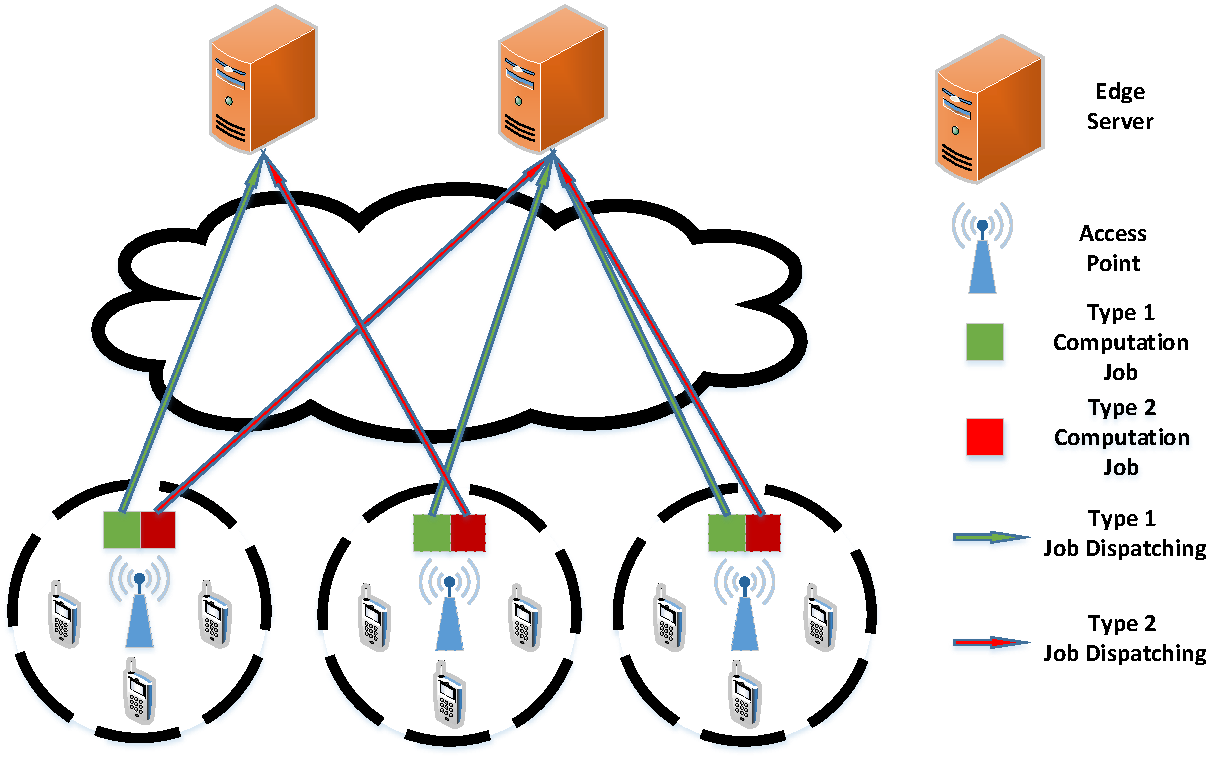
\includegraphics[width=1.0\textwidth]{chapter3_prev/system-model.pdf}
    \caption{Illustration of the edge computing network.}
    \label{fig:ch3_prev-system}
\end{figure*}

Finally, MDP is a powerful tool for resource allocation of communication networks with random transition of system state. For example,  
infinite-horizon average cost MDP has been used in delay-aware radio resource management \cite{Ruiwang2011,Cui2012,Ruiwang2013}. Joint optimization of file placement and delivery in cache-assisted wireless networks can be solved via finite-horizon MDP \cite{Lv2018-icc,Lv2018-gc,Lv2019}. Various value function approximation methods have been used in \cite{Ruiwang2011,Cui2012,Ruiwang2013,Lv2018-icc,Lv2018-gc,Lv2019} 
to address the \emph{curse of dimensionality}. However, there is no analytical performance bound on the proposed approximation algorithms.

In this chapter, we would like to shed some lights on the above issue by optimizing the job dispatching from multiple APs to multiple edge servers via a network with unpredictable uploading delay.
Specifically, we consider the \emph{unrelated machines model} so that different edge servers may have different processing capability on each job type. 
The job arrivals, job uploading delay from APs to edge servers and the job computation time at the edge servers are all modeled via random variables.
Our contributions in this job dispatching scenario are summarized below.
\begin{itemize}
    \item We formulate the joint optimization of job dispatching in all the APs and time slots as an infinite-horizon MDP, where the minimization objective is a discounted measurement of job processing time, including the uploading delay, the waiting time and the computation time  at
        edge servers. The issue of random uploading delay and computation time is addressed via the state transition distribution of MDP formulation.
    \item Conventional MDP problems suffer from \emph{curse of dimensionality}.
    In order to address this issue, a novel approach of value function approximation is proposed for the above infinite-horizon MDP with discounted cost, where the expressions of approximated value function is derived. Hence, the complicated value iteration is avoided. Moreover, with this new approach, the performance of the proposed dispatching algorithm can be analytically bounded. 
\end{itemize}

We use the following notations throughout this chapter:
$\mathbb{G}(p)$ denotes the geometric distribution with parameter $p$;
$\mathbb{B}(n,p)$ denotes binomial distribution with parameters $n$ and $p$;
$\mathbb{R}^{M\times N}$ denotes spaces of $M\times N$ matrices with real entries.
The remainder of this chapter is organized as follows.
The system model is presented in Section \ref{sec:chapter3_prev-model}.
Problem formulation and low-complexity scheduling are illustrated in Section \ref{sec:chapter3_prev-formulation} and Section \ref{sec:chapter3_prev-solution}, respectively.
In Section \ref{sec:chapter3_prev-simulation}, numerical simulations are conducted.
Finally, the conclusion is drawn in Section \ref{sec:chapter3_prev-conclusion}.

%=================================================================================================%
%=================================================================================================%

\section{System Model}
\label{sec:chapter3_prev-model}
In this section, we introduce the model of the edge computing system considered, including the statistical models of job arrival, uploading and computation.

\subsection{Network Model}
We consider an edge computing system with $K$ access points (APs) and $M$ edge servers, which are connected in a network as illustrated in \figurename~\ref{fig:ch3_prev-system}. The sets of APs and edge servers are denoted as $\apSet \define \set{1, \dots, K}$ and
$\esSet \define \set{1, \dots, M}$, respectively.
Each AP collects the computation jobs from the mobile users within its service area, and uploads each job to one of the edge servers.
Without loss of generality, it is assumed that there are $J$ types of computation jobs supported in this system, which are denoted via the set $\jSpace \define \set{1, \dots, J}$.
The edge servers may have different processing capability on different job types. The APs and edge servers may be deployed in an open network (e.g., metropolitan area network) with other traffics (e.g., video streaming and file delivery).
It is shown in a number of existing literature \cite{tan-online,liang2017} that the job uploading delay is not negligible compared with the computation time. Moreover, due to the randomness of network traffics, the job uploading delay is assumed to be random. We shall optimize the computation edge server for each job type at the APs, according to the distribution of job uploading delay, the queuing status and the job processing capability of edge servers. 

The time axis is organized by time slots in order to facilitate the dispatcher design. The job arrival in each time slot is modelled via Bernoulli distribution. Specifically, the arrivals of the $j$-th job type at the $k$-th AP in different time slots are independent and identically distributed (i.i.d.) Bernoulli random variables, and the arrival probability is denoted as $\lambda_{k,j}$ ($\forall k\in\apSet, j\in\jSpace$). Let $A_{k,j}(t)\in\set{0,1}$ be the indicator of job arrival, where $A_{k,j}(t)=1$ means one job of the  $j$-th type arrives at the $k$-th AP in the $t$-th time slot, and $A_{k,j}(t)=0$ means otherwise. Hence,
\begin{align}
    \Pr\Paren{ A_{k,j}(t)=1 } = \lambda_{k,j}, \forall k,j,t.
\end{align}

At the beginning of each time slot, APs dispatch each type of jobs arrived in the previous time slot to one edge server. Thus, the APs make decisions on the mapping from job types to edge servers in each time slot. We shall refer to these decisions in each time slot as dispatching actions. Let $\omega_{k,j}(t)\in\esSet$ denotes the index of edge server, to which the $k$-th AP dispatches the job of the $j$-th type in the $t$-th time slot. The dispatching action of the system in the t-th time slot can be represented as
\begin{align*}
    \set{ \omega_{k,j}(t)|\forall k\in\apSet,\forall j\in\jSpace }.
\end{align*}

Different types of jobs may have different distributions on the input data size. Moreover, the network between APs and edge servers may be jammed by other traffics. The job uploading delay from one AP to one edge server cannot be predicted accurately by APs. Instead, it is assumed that the uploading delay follows independent geometric distribution. Denote the geometric delay distribution of the $j$-th job type from the $k$-th AP to the $m$-th edge server as $\mathbb G\left(1/\bar{U}_{k,j}^{m}\right)$, where $\bar{U}_{k,j}^{m}$ is the expectation of the distribution. 

\begin{remark}[Memoryless Uploading Delay Distribution]
    The  geometric distribution has the memoryless property. For example, let $U^m_{k,j}(t)$ be the uploading delay of the job of the $j$-th type which is dispatched from the $k$-th AP to the $m$-th edge sever in the $t$-th time slot. Then,
    $\forall n>0, s>0, t, k\in\apSet,j\in\jSpace,m\in\esSet$, 
    \begin{align*}
        \Pr\Paren{
            {U}_{k,j}^{m}(t)> n+s\big|{U}_{k,j}^{m}(t)>n
        } = 
        \Pr\Paren{{U}_{k,j}^{m}(t)>s}.
    \end{align*}
    As a result, the statistics of job arrivals at the edge servers depend only on the number of jobs which are being delivered from APs to edge servers. It is not necessary for the APs to record the number of time slots for which these jobs has been delivered from the AP.
    However, our proposed algorithm is not limited to the geometric delay distribution. It can be easily extended to the scenarios that the job uploading delay follows other distributions. We use the geometric distribution as it can simplify the notation system.
\end{remark}

Let $N_{k,j}^m(t)$ be the number of the jobs of the $j$-th type, which is being uploaded from the $k$-th AP to the $m$-th edge server at the beginning of the $t$-th time slot, $D_{k,j}^m(t)\in\set{0,1,\dots,N_{k,j}^m(t)}$ be the number of the jobs of the $j$-th type which arrive at the $m$-th edge server from the $k$-th AP in the $t$-th time slot, respectively.
As a remark notice that the data of the jobs in $N_{k,j}^m(t)$ have not arrived at the $m$-th edge server by the beginning of the $t$-th time slot. Due to the random uploading delay, some of these jobs may arrive during the $t$-th time slot, which are measured by $D_{k,j}^m(t)$. Hence, $D_{k,j}^m(t)$ follows binomial distribution with expectation $N_{k,j}^m(t)/\bar{U}_{k,j}^{m}$, i.e., $D_{k,j}^m(t)\sim \mathbb{B}(N_{k,j}^m(t),1/\bar{U}_{k,j}^{m})$,
and the probability mass function (PMF) of $D_{k,j}^m(t)$ is given by
\begin{align}
\Pr\left(D_{k,j}^m(t)=n\right)&=\binom{N_{k,j}^m(t)}{n}\left(\frac{1}{\bar{U}_{k,j}^{m}}\right)^n\left(1-\frac{1}{\bar{U}_{k,j}^{m}}\right)^{N_{k,j}^m(t)-n}, \nonumber\\ 
\forall n&=0,1,\dots,
N_{k,j}^m(t).
\end{align}
Hence, given job arrival process $A_{k,j}(t)$ and job dispatching decision $\omega_{k,j}(t)$,  the dynamics of $N_{k,j}^m(t+1)$ ($\forall t, k\in \apSet, m\in \esSet, j \in \jSpace$)  can be expressed as
\begin{align}
N_{k,j}^m(t+1)=&N_{k,j}^m(t)+A_{k,j}(t)\indicator[\omega_{k,j}(t)=m]-D_{k,j}^m(t).
\end{align}
In the above equation, $\indicator[\mathcal{E}]$ is the indicator function, whose value is $1$ when the event $\mathcal{E}$ is true and $0$ otherwise.

\subsection{Computation Model}
There are $J$ virtual machines (VMs) on each edge server for the computation of $J$ job types, respectively. For each type, the uploaded jobs are computed in a first-come-first-serve (FCFS) manner.
Hence, a processing queue with maximum $L_{\max}$ jobs is established for each VM, and the first job is computed. The arrival jobs will be discarded when the processing queue is full.
Denote $L_{m,j}(t)\in\set{0,1,\dots,L_{{\max}}}$ as the number of the jobs of the $j$-th type at the $m$-th edge server at the beginning of the $t$-th time slot.

We adopt the \emph{unrelated machines} assumption as in \cite{tan-online} for job computation on edge servers. Specifically, it is assumed that different types of jobs have different distributions of computation time at each edge server.
We denote $f_{m,j}(x)$ as the PMF of computation time distribution of the j-th job type at the m-th edge server ($\forall m\in\esSet, j \in \jSpace$).
Let $\eta_{m,j}(t)\in\{0,1,\dots,\eta_{{\max}}\}$ be the remaining computation time slots of the first job at the $j$-th VM at the beginning of the $t$-th time slot, where $\eta_{{\max}}$ denotes the maximum number of computation time slots for each job. Then dynamics of  $\set{\eta_{m,j}(t)|\forall t}$ are summarized below: 
\begin{itemize}
    \item When the $\eta_{m,j}(t)>1$,  $\eta_{m,j}(t+1)=\eta_{m,j}(t)-1$;
    \item When the computation of the first job is finished in the $t$-th time slot ($ \eta_{m,j}(t)= \{0,1\} $) and there are no job in the processing queue ($ L_{m,j}(t)=0 $), ${\eta}_{m,j}(t+1)=0$;
    \item When the computation of the current job is finished in or before the $t$-th time slot ($ \eta_{m,j}(t)= 1 $) and $ L_{m,j}(t)>0 $, the distribution of $\eta_{m,j}(t+1)$ is given by 
    \begin{align}
    \Pr\Paren{ \eta_{m,j}(t+1)=x } = f_{m,j}(x), \forall t, x\in \set{0,1,\dots,L_{{\max}}}.
    \end{align}
\end{itemize}
Moreover, the dynamics of $L_{m,j}(t)$ can be expressed as
\begin{align}
    L_{m,j}(t+1) = \min\Paren{
        L_{m,j}(t) - \indicator[\eta_{m,j}(t)=1] + \sum_{\forall k \in \apSet}D_{k,j}^m(t), L_{{\max}}
    },
    \nonumber\\ 
    \forall t, m\in\esSet,j\in\jSpace.
\end{align}
 
In the remaining of this chapter, we shall refer to
$
Q_{m,j}(t) \define \Paren{ L_{m,j}(t), \eta_{m,j}(t) }
$
as the queuing state information (QSI) of the $j$-th type job at the $m$-th edge server at the beginning of the $t$-th time slot.

%=================================================================================================%
%=================================================================================================%

\section{Infinite-Horizon MDP Formulation}
\label{sec:chapter3_prev-formulation}
Since the job dispatching in one time slot will affect the system status (e.g., QSI of the edge servers) of the following time slots.
The joint optimization of job dispatching in all the time slots is necessary. In this section, we shall formulate such joint optimization as a MDP. 

\subsection{System State and Scheduling Policy}
We first define the system state $\Stat$ and scheduling policy $\Policy$ as follows. 
\begin{definition}[System State] \em
    At the beginning of the $t$-th time slot, the system state of the $j$-th job type is represented as $\Stat_j(t) \define (\mathbf{N}_j(t),\mathbf{Q}_j(t))$, which consists of
    \begin{itemize}
        \item The number of jobs being uploaded:
        \begin{align}
        \mathbf{N}_j(t) \define \{N_{k,j}^m(t)|\forall k \in \apSet, \forall m \in \esSet \};
        \end{align}
        \item Queuing state information (QSI) of the edge servers:
        \begin{align}
        \mathbf{Q}_j(t) \define \{Q_{m,j}(t)|\forall m \in \esSet\}.
        \end{align}
    \end{itemize}
    Moreover, the aggregation of system state of all the type of jobs is referred to as the system state $\Stat(t)$, i.e., $\Stat(t) \define \{\Stat_j(t) | \forall j\in\jSpace \}$.
\end{definition}

It is assumed that all the APs and edge servers will broadcast their latest status at the end of every time slot, and the APs are able to collect the complete system state at the beginning of each time slot (i.e., $\Stat(t)$ at the beginning of the $t$-th time slot), so that the decision on job dispatching can be made accordingly. We ignore the delay of system state broadcasting, as the message size is small. Hence, the job dispatching policy is defined below.
\begin{definition}[Job Dispatching Policy] \em
     In the $t$-th time slot, the dispatching policy of the $j$-th job type, denoted as $\Policy_j$, is a mapping from system state $\Stat(t)$ to the job dispatching action  $\{ \omega_{k,j}(t)|\forall k\in\apSet \}$, i.e.,
        \begin{align}
        \Policy_{j}(\Stat(t)) \define \{\omega_{k,j}(t)|\forall k\in\apSet\}, \forall t.
        \end{align}
    Moreover, the aggregation of dispatching policies of all the job types is referred to as the system dispatching policy $\Policy$, i.e., $\Policy \define \{\Policy_j | \forall j\in\jSpace \}$.
\end{definition}

\subsection{Problem Formulation}
According to the Little's law, the average processing time per job of the edge computing system, measuring the number of time slots from job arrival to the completeness of computation, is proportional to the average number of jobs in the system. We use the discounted summation of job numbers in all the time slots as the approximation of average processing time. Specifically, we first define the following weighted sum of the job number and job overflow penalty as the system cost at the $t$-th time slot.
{\small
\begin{align}
    &g\Paren{ \Stat(t),\Policy(\Stat(t)) }
        \define \sum_{j\in\jSpace} \Brace{
            \underbrace{\sum_{k\in\apSet}\sum_{m\in\esSet}N_{k,j}^m(t) +\sum_{m\in\esSet}\Paren{
                L_{m,j}(t) + \beta \indicator[L_{m,j}(t)=L_{{\max}}]
            }}_{g_j\Paren{ \Stat_j(t),\Policy_j(\Stat_{j}(t)) }}
        },
\end{align}
}
where $\beta$ is a weight, and $g_j(\Stat_j(t),\Policy_j(\Stat_{j}(t)))$ denotes the system cost of $j$-th type in the $t$-th time slot. The overall system cost of all the time slots with the initial system state $\Stat$ is then given by
\begin{align}
    \bar{G}(\Policy, \Stat) \define
    \lim\limits_{T\to\infty} \mathbb{E}_{\{\Stat(t)|\forall t\}}^{\Policy}
    \Bracket{
        \sum_{t=1}^{T} \gamma^{t-1}g\Paren{\Stat(t),\Policy(\Stat(t))} \big|
        \Stat(1)=\Stat
    },
\end{align}
where $\mathbb{E}_{\{\Stat(t)|\forall t\}}^{\Policy}[.]$ denotes the expectation with respect to all possible system states in the future given dispatching policy $\Policy$, and $\gamma$ is the discount factor. As a result, the cooperative job dispatching design can be formulated as the following infinite-horizon MDP.
\begin{problem}[Cooperative Job Dispatching Problem]\label{Pro:main} \em
    \begin{align}
            \Policy^*&=\mathop{\arg\min}_{\Policy} \bar{G}(\Policy,\Stat) .
    \end{align}
\end{problem}
The optimal policy of Problem \ref{Pro:main} can be obtained by solving the following Bellman's equations \cite{dp-control},
\begin{align}
    \label{eqn:bellman}
    V(\Stat(t)) = \min_{\Policy(\Stat(t))} g\Paren{ \Stat(t),\Policy(\Stat(t)) }
    +\gamma \sum_{\Stat(t+1)} &\Pr\Paren{ \Stat(t+1)\big|\Stat(t),\Policy(\Stat(t)) }
    \nonumber\\
    &\times V\Paren{ \Stat(t+1) },
    \forall \Stat(t),
\end{align}
where $V(\cdot)$ denotes the value function of the optimal policy $\Policy^*$. It is proven in \cite{dp-control} that, $V(\Stat)$ represents the average system cost with initial system state $\Stat$ and optimal scheduling policy $\Policy^{*}$, i.e.,
\begin{eqnarray*}
    V(\Stat) = \lim\limits_{T\to\infty} \mathbb{E}_{\{\Stat(t)|\forall t\}}^{\Policy^{*}}
    \Bracket{
        \sum_{t=1}^{T} \gamma^{t-1}g\Paren{ \Stat(t),\Policy^{*}(\Stat(t)) }\big|\Stat(1)=\Stat
    }.
\end{eqnarray*}
The system state transition probability can be written as
\begin{align}\label{eqn:decouple}
    &\Pr\Paren{ \Stat(t+1)\big|\Stat(t),\Policy(\Stat(t)) }
    =\prod_{j\in\jSpace}\Pr\Paren{  \Stat_j(t+1)\big|\Stat_j(t),\Policy_j(\Stat_j(t))}
    \nonumber\\
    =&\prod_{j\in \jSpace,\forall k \in \apSet, \forall m \in \esSet}\Pr\Paren{ N_{k,j}^m(t+1)\big|\Stat_j(t),\Policy_j(\Stat_j(t)) }
    \nonumber\\
    &\times\prod_{j\in \jSpace,\forall m \in \esSet}\Pr\Paren{ Q_{m,j}(t+1)\big|\Stat_j(t),\Policy_j(\Stat_j(t)) }.
\end{align}

Generally speaking, the standard value iteration can be used to solve the value function $V(.)$ for all possible system states, and the optimal policy denoted as $\Policy^{*}$, can be derived by solving the minimization problem of the right-hand-side of the  Bellman's equations in Equation \eqref{eqn:bellman}. In our problem, however, the conventional value iteration is intractable due to the tremendous state space. For example, the number of system states grows exponentially with respect to the number of APs and edge servers. Hence, a novel low-complexity sub-optimal solution is proposed in the following section, whose performance can be bounded analytically. As a remark notice that it is difficult to obtain an analytical bound for the existing approximate MDP solution methods as in \cite{Ruiwang2011,Cui2012,Ruiwang2013}.

%=================================================================================================%
%=================================================================================================%

\section{Low-Complexity Scheduling Policy}
\label{sec:chapter3_prev-solution}
In this section, we first introduce a heuristic scheduling policy as the baseline policy, whose value functions are derived analytically. Then, the proposed low-complexity sub-optimal policy can be obtained via the above value function and one-step policy iteration. The derived value function of the baseline policy becomes the cost upper bound of the proposed sub-optimal policy.

\subsection{Baseline Scheduling Policy}
The baseline scheduling policy with fixed dispatching action is elaborated below.
\begin{policy}[Baseline Scheduling Policy $\Baseline$]
    \label{Pol:baseline} \em
    The following dispatching policy $\Baseline$ is adopted as the baseline policy.
    \begin{align}
    \Baseline \define \{\omega_{k,j}(t)=\omega_{k,j}^{\Baseline}|\forall t,k,j\},
    \end{align}
    where $\omega_{k,j}^{\Baseline}\in\esSet$ denotes the index of the fixed edge server for the processing of the $j$-th job type from the $k$-th AP.
\end{policy}

Given the system state $\Stat$ in the first time slot, the value function of policy $\Baseline$ is defined as
\begin{align}
    V_{\Baseline}(\Stat)\define \lim\limits_{T\to\infty} \mathbb{E}_{\{\Stat(t)|\forall t\}}^{\Baseline} \Bracket{
        \sum_{t=1}^{T} \gamma^{t-1}g(\Stat(t),\Baseline)\big|\Stat(1)=\Stat
    }.
\end{align}
In order to derive its analytical expression, we let 
\begin{align}
    {d}_{k,j,m}^{\text{AP}}(N_{k,j}^m) \define \lim\limits_{T\to\infty} \mathbb{E}^{\Baseline}_{\{N_{k,j}^{m}(t)|\forall t\}} \Bracket{
        \sum_{t=1}^{T}\gamma^{t-1}N_{k,j}^{m}(t)\big|N_{k,j}^{m}(1)=N_{k,j}^{m}
    }
\end{align}
be the average cost raised by the jobs of the $j$-th type which is being uploaded from $k$-th AP to $m$-th server, and 
\begin{align}
    {d}_{m,j}^{\text{ES}}(\Stat_j)\define &\lim\limits_{T\to\infty} \mathbb{E}^{\Baseline}_{\{N_{k,j}^{m}(t)|\forall t\}}\Bracket{
        \sum_{t=1}^{T} \gamma^{t-1}L_{m,j}(t)
        + \beta \indicator[L_{m,j}(t)=L_{\max}]\big|\Stat_j(1)=\Stat_j
    }
\end{align}
be the average cost raised by jobs of the $j$-th type at the $m$-th edge server. $V_{\Baseline}(\Stat)$ can be written as 
\begin{align}\label{eqn:V_baseline}
    V_{\Baseline}(\Stat) = \sum_{j\in\jSpace}\Paren{
        \underbrace{\sum_{k\in\apSet}\sum_{m\in\esSet}{d}_{k,j,m}^{\text{AP}}(N_{k,j}^{m})
        +\sum_{m\in\esSet}{d}_{m,j}^{\text{ES}}(\Stat_j)}_{W_{j}(\Stat_j)}
    },
\end{align}
where the expressions of ${d}_{k,j,m}^{\text{AP}}(.)$ and ${d}_{m,j}^{\text{ES}}(.)$ are given by following two lemmas respectively.

\begin{table*}
    \centering
    \caption{Entries of matrix $\mathbf{M}_{k,j,m}$}
    \label{table:M_{k,j,m}}
    \begin{tabular}{ |p{0.27\linewidth}|p{0.27\linewidth}|p{0.46\linewidth}| }  
        \hline
        & & \\[-6pt]
        $q$&$p$&$[\mathbf{M}_{k,j,m}]_{q,p}$ \\
        \hline
        & &  \\[-6pt]
        $0$&$0$&$1-\lambda_{k,j}$ \\
        \hline
        & &  \\[-6pt]
        $0$&$1$&$\lambda_{k,j}$ \\
        \hline
        & &  \\[-6pt] 
        $0$&$2,\dots,N_{\max}$&$0$ \\
        \hline
        & &  \\[-6pt] 
        $a\in\{1,\dots,N_{\max}-1\}$ & $b\in\{0,\dots,a\}$ & $(1-\lambda_{k,j})\binom{a}{a-b}(\frac{1}{\bar{U}_{k,j}^{m}})^{a-b}(1-\frac{1}{\bar{U}_{k,j}^{m}})^{b}+\lambda_{k,j}\binom{a}{a-b+1}(\frac{1}{\bar{U}_{k,j}^{m}})^{a-b+1}(1-\frac{1}{\bar{U}_{k,j}^{m}})^{b-1}$ \\
        \hline
        & &  \\[-6pt] 
        $a\in\{1,\dots,N_{\max}-1\}$&$a+1$&$\lambda_{k,j}(1-\frac{1}{\bar{U}_{k,j}^{m}})^{a}$ \\
        \hline
        & &  \\[-6pt] 
        $a\in\{1,\dots,N_{\max}-1\}$&$b\in\{a+2,\dots,N_{\max}\}$&$0$ \\
        \hline
        & &  \\[-6pt] 
        $N_{\max}$&$b\in\{0,\dots,N_{\max}-1\}$&${(1-\lambda_{k,j})\binom{N_{\max}}{N_{\max}-b}(\frac{1}{\bar{U}_{k,j}^{m}})^{N_{\max}-b}(1-\frac{1}{\bar{U}_{k,j}^{m}})^{b}\atop+\lambda_{k,j}\binom{N_{\max}}{N_{\max}-b+1}(\frac{1}{\bar{U}_{k,j}^{m}})^{N_{\max}-b+1}(1-\frac{1}{\bar{U}_{k,j}^{m}})^{b-1}}$ \\
        \hline
        & &  \\[-6pt] 
        $N_{\max}$ & $N_{\max}$ & $(1-\lambda_{k,j})(1-\frac{1}{\bar{U}_{k,j}^{m}})^{N_{\max}}+\lambda_{k,j}{N_{\max}}(\frac{1}{\bar{U}_{k,j}^{m}})(1-\frac{1}{\bar{U}_{k,j}^{m}})^{N_{\max}-1}+\lambda_{k,j}(1-\frac{1}{\bar{U}_{k,j}^{m}})^{N_{\max}}$ \\
        \hline
    \end{tabular}
\end{table*}

\begin{lemma}[Analytical Expression of ${d}_{k,j,m}^{\text{AP}}$]
    \label{lemma:AP}\em
    ${d}_{k,j}^{\text{AP}}(N_{k,j}^m)$ can be expressed as
    \begin{align}\label{eqn:AP}
    {d}_{k,j,m}^{\text{AP}}(N_{k,j}^m)&=	\sum_{t=1}^{+\infty}[\mathbf{u}_{k,j,m}(N_{k,j}^m)]^{\mathsf{T}}(\gamma\mathbf{M}_{k,j,m})^{t-1}\mathbf{g}\nonumber\\
    &=[\mathbf{u}_{k,j,m}(N_{k,j}^m)]^{\mathsf{T}}(\mathbf{I}-\gamma\mathbf{M}_{k,j,m})^{-1}\mathbf{g},
    \end{align}
    where the notations of $\mathbf{u}_{k,j,m}(N_{k,j}^m)$, $\mathbf{g}$ and $\mathbf{M}_{k,j,m}$ are defined below.
    \begin{itemize}
        \item $\mathbf{u}_{k,j,m}(N_{k,j}^m)\in \mathbb{R}^{(N_{\max}+1)\times1}$, whose $N_{k,j}^m$-th entry is $1$ and other entries are all $0$.
        \item $\mathbf{g}\in \mathbb{R}^{(N_{\max}+1)\times1}$, whose $i$-th entry is $i$, $i=0,1,\dots,N_{\max}$.
        \item $\mathbf{M}_{k,j,m}\in \mathbb{R}^{(N_{\max}+1)\times(N_{{\max}}+1)}$ denotes the transition matrix of the $\{N_{k,j}^m(t)|\forall t\}$, whose entries are given in Table \ref{table:M_{k,j,m}}.
    \end{itemize}
\end{lemma}
\begin{proof}
    The entries of matrix $\mathbf{M}_{k,j,m}$ is
    \begin{align*}
        [\mathbf{M}_{k,j,m}]_{q,p}\define\Pr\Paren{ N_{k,j}^m(t+1)=p\big|N_{k,j}^m(t)=q,\Baseline }.
    \end{align*}
    Then, we have following discussion on $[\mathbf{M}_{k,j,m}]$.
    \begin{itemize}
        \item $q=0$, $p=0$: There are no $j$-th type job arriving at the $k$-th AP. Hence $[\mathbf{M}_{k,j,m}]_{0,0}=1-\lambda_{k,j}$.
        \item $q=0$, $p=1$: There is one $j$-th type job arriving at the $k$-th AP. Hence $[\mathbf{M}_{k,j,m}]_{0,1}=\lambda_{k,j}$.
        \item $q=a\in\{1,\dots,N_{{\max}}-1\}$, $p=b\in\{0,\dots,a\}$: (i)
        There are no $j$-th type job arriving at the $k$-th AP and $D_{k,j}^{m}(t)=(a-b)$; (ii) There is one $j$-th type job arriving at the $k$-th AP and $D_{k,j}^{m}(t)=(a-b)-1$.
        Hence,  $[\mathbf{M}_{k,j,m}]_{a,b}=(1-\lambda_{k,j})\binom{a}{a-b}(\frac{1}{\bar{U}_{k,j}^{m}})^{a-b}(1-\frac{1}{\bar{U}_{k,j}^{m}})^{b}+\lambda_{k,j}\binom{a}{a-b+1}(\frac{1}{\bar{U}_{k,j}^{m}})^{a-b+1}(1-\frac{1}{\bar{U}_{k,j}^{m}})^{b-1}$.
        \item $ q=a\in\{1,\dots,N_{{\max}}-1\}$, $p=a+1$: There is one $j$-th type job arriving at the $k$-th AP and  $D_{k,j}^{m}(t)=0$. Hence, $[\mathbf{M}_{k,j,m}]_{a,a+1}=\lambda_{k,j}(1-\frac{1}{\bar{U}_{k,j}^{m}})^{a}$.
        \item  $q=N_{\max}$, $p=b\in\{0,\dots,N_{\max}-1\}$: (i)
        There are no $j$-th type job arriving at the $k$-th AP and $D_{k,j}^{m}(t)=(N_{{\max}}-b)$; (ii) There is one $j$-th type job arriving at the $k$-th AP and $D_{k,j}^{m}(t)=(N_{{\max}}-b)-1$. Hence, $[\mathbf{M}_{k,j,m}]_{N_{{\max}},b}=(1-\lambda_{k,j})\binom{N_{\max}}{N_{\max}-b}(\frac{1}{\bar{U}_{k,j}^{m}})^{N_{\max}-b}(1-\frac{1}{\bar{U}_{k,j}^{m}})^{b}+\lambda_{k,j}\binom{N_{\max}}{N_{\max}-b+1}(\frac{1}{\bar{U}_{k,j}^{m}})^{N_{\max}-b+1}(1-\frac{1}{\bar{U}_{k,j}^{m}})^{b-1}$.
        \item  $q=N_{\max}$, $p=N_{\max}$: (i)There are no $j$-th type job arriving at the $k$-th AP and $D_{k,j}^{m}(t)=0$; (ii) There is one $j$-th type job arriving at the $k$-th AP and $D_{k,j}^{m}(t)=1$; There is one $j$-th type job arriving at the $k$-th AP and $D_{k,j}^{m}(t)=0$. Hence, $[\mathbf{M}_{k,j,m}]_{N_{{\max}},N_{{\max}}}=(1-\lambda_{k,j})(1-\frac{1}{\bar{U}_{k,j}^{m}})^{N_{\max}}+\lambda_{k,j}{N_{\max}}(\frac{1}{\bar{U}_{k,j}^{m}})(1-\frac{1}{\bar{U}_{k,j}^{m}})^{N_{\max}-1}+\lambda_{k,j}(1-\frac{1}{\bar{U}_{k,j}^{m}})^{N_{\max}}$.
        \item Otherwise, $[\mathbf{M}_{k,j,m}]_{q,p}=0$.
    \end{itemize}

    To prove the second equity of Equation \eqref{eqn:AP}, we first show $||\gamma\mathbf{M}_{k,j,m}||<1$, where $||.||$ is the matrix norm. It clear that $||\gamma\mathbf{M}_{k,j,m}||=\gamma\rho(\mathbf{M}_{k,j,m})$, where $\rho(\mathbf{M}_{k,j,m})$ is the spectrum radius of  $\mathbf{M}_{k,j,m}$. According to Perron-Frobenius Theorem \cite{meyer2000matrix}, the spectrum radius of transition probability matrix is $1$. Since $\mathbf{M}_{k,j,m}$ is transition probability matrix, we have $||\gamma\mathbf{M}_{k,j,m}||=\gamma<1$. Let $\mathbf{X}_n=\sum_{t=1}^{n}(\gamma\mathbf{M}_{k,j,m})^{t-1}$, we have
    \begin{align*}
        \mathbf{X}_n=(\mathbf{I}-\gamma\mathbf{M}_{k,j,m})^{-1}-(\gamma\mathbf{M}_{k,j,m})^{n+1}(\mathbf{I}-\gamma\mathbf{M}_{k,j,m})^{-1}.
    \end{align*}
    Then
    \begin{align*}
        \lim\limits_{n\to+\infty} \mathbf{X}_n=(\mathbf{I}-\gamma\mathbf{M}_{k,j,m})^{-1}.
    \end{align*}
    Hence, the Equation \eqref{eqn:AP} is straightforward.
\end{proof}


\begin{lemma}[Analytical Expression of ${d}_{m,j}^{\text{ES}}$]
    \label{lemma:ES}
    ${d}_{m,j}^{\text{ES}}(\Stat_j)$ is given by
    \begin{align}
    {d}_{m,j}^{\text{ES}}(\Stat_j)=&[\mathbf{q}_{m,j}(Q_{m,j})]^{\mathsf{T}}\mathbf{c}\nonumber\\
    &+\sum_{t=2}^{+\infty}[\mathbf{q}_{m,j}(Q_{m,j})]^{\mathsf{T}}\Big[\gamma\mathbf{P}_{m,j}\Big(\alpha_{m,j}(t-1)\Big)\Big]^{t-1}\mathbf{c},
    \end{align}
    where the notations of $\mathbf{q}_{m,j}({Q}_{m,j})$,  $\mathbf{c}$, $\mathbf{P}_{m,j}\Big(\alpha_{m,j}(t-1)\Big)$ and $\alpha_{m,j}(t-1)$ are defined below.
    \begin{itemize}
        \item $\mathbf{q}_{m,j}({Q}_{m,j})\in \mathbb{R}^{(L_{{\max}}\eta_{{\max}}+1)\times1}$, whose $i$-th entry is 
            \begin{align}
        [\mathbf{q}_{m,j}({Q}_{m,j})]_{i}=\begin{cases}
        1, & i=\eta_{m,j}+(L_{m,j}-1)*\eta_{{\max}}
        \cr
    0, & 
            i=0,\dots,\eta_{m,j}+(L_{m,j}-1)*\eta_{{\max}}-1,\atop\eta_{m,j}+(L_{m,j}-1)*\eta_{{\max}}+1,\dots,\eta_{{\max}}L_{{\max}}
        \end{cases}
        \end{align}
        \item $\mathbf{c}\in \mathbb{R}^{(L_{{\max}}\eta_{{\max}}+1)\times1}$,  whose $i$-th entry is 
        \begin{align}
        c_{i}=\begin{cases}
        \lceil i/\eta_{{\max}}\rceil, & i=0,1,\dots,(L_{{\max}}-1)\eta_{{\max}}
        \cr
        L_{{\max}}+\beta, & \text{ otherwise}
        \end{cases}
        \end{align}
        \item $\mathbf{P}_{m,j}\Big(\alpha_{m,j}(t-1)\Big)\in\mathbb{R}^{(L_{{\max}}\eta_{{\max}}+1)\times(L_{{\max}}\eta_{{\max}}+1)}$ denotes the transition matrix of the $\{Q_{m,j}(t)|\forall t\}$ given the average number of job arrival $\alpha_{m,j,t-1}$, where
        \begin{align}
        \alpha_{m,j}(t)\triangleq\sum_{k\in\apSet} \indicator(\omega_{k,j}^{\Baseline}=m)\frac{[\mathbf{u}_{k,j,m}(N_{k,j}^m)]^{\mathsf{T}}(\mathbf{M}_{k,j,m})^{t-1}\mathbf{g}}{\bar{U}_{k,j}^m}.
        \end{align}
        The entries of the transition probability matrix $\mathbf{P}_{m,j}(.)$ are provided by table \ref{table:P}.
    \end{itemize}
\end{lemma}
\begin{proof}
    The proof is similar to the proof of Lemma \ref{lemma:AP}.
\end{proof}

\begin{table*}
    \centering
    \caption{Entries of matrix $[\mathbf{P}_{m,j}(\alpha_{m,j}(t-1))]$}
    \label{table:P}
    \begin{tabular}{ |p{0.40\linewidth}|p{0.33\linewidth}|p{0.27\linewidth}| }
        \hline
        & & \\[-6pt]
        $q$ & $p$ & $[\mathbf{P}_{m,j}(\alpha_{m,j}(t-1))]_{q,p}$\\
        \hline
        & & \\[-6pt]
        $0$&$0$&$1-\alpha_{m,j}(t-1)$\\  %
        \hline
        & & \\[-6pt]
        $0$ & $b\in\{1,\dots,N_{{\max}}\}$ & $(1-\alpha_{m,j}(t-1))f_{m,j}(b)$\\  %
        \hline
            & & \\[-6pt]
        $0$&$\{N_{{\max}}+1,\dots,Q_{{\max}}N_{{\max}}\}$&$0$\\  %
        \hline
            & & \\[-6pt]
        $a\in\{N\times N_{{\max}}+2,\dots,N\times N_{{\max}}+N_{{\max}}|N=0,1,\dots,Q_{{\max}}-1\}$&$a-1$&$1-\alpha_{m,j}(t-1)$\\  %
        \hline
        & & \\[-6pt]
        $a\in\{N\times N_{{\max}}+2,\dots,N\times N_{{\max}}+N_{{\max}}|N=0,1,\dots,Q_{{\max}}-1\}$&$a+N_{{\max}}-1$&$\alpha_{m,j}(t-1)$\\  %
        \hline
        & & \\[-6pt]
        $a\in\{N\times N_{{\max}}+2,\dots,N\times N_{{\max}}+N_{{\max}}|N=0,1,\dots,Q_{{\max}}-1\}$&${\{1,\dots,N_{{\max}}Q_{{\max}}\}\atop\setminus\{a-1,a+N_{{\max}}-1\}}$&$0$\\  %
        \hline
            & & \\[-6pt]
        $a\in\{N\times N_{{\max}}+1|N=0,1,\dots,Q_{{\max}}-1\}$&$b\in\{a-N_{{\max}},\dots,a-1\}$&${(1-\alpha_{m,j}(t-1))\atop\times f_{m,j}(b-a+1+N_{{\max}})}$\\  %
        \hline
            & & \\[-6pt]
        $a\in\{N\times N_{{\max}}+1|N=0,1,\dots,Q_{{\max}}-1\}$&$b\in\{a,\dots,a-1+N_{{\max}}\}$&${(1-\alpha_{m,j}(t-1))\atop\times f_{m,j}(b-a+1)}$\\  %
        \hline
            & & \\[-6pt]
        $a\in\{N\times N_{{\max}}+1|N=0,1,\dots,Q_{{\max}}-1\}$&${\{1,\dots,N_{{\max}}Q_{{\max}}\}\setminus\atop\{\{a-N_{{\max}},\dots,a-1\}\cup \{a,\dots,a-1+N_{{\max}}\}\}}$&$0$\\  %
        \hline
    \end{tabular}
\end{table*}

\subsection{Scheduling Policy with One-Step Policy Iteration}
In this section, we use the value function of the baseline policy $\{V_{\Baseline}(\Stat)|\forall \Stat\}$ derived in the previous section to approximate the value function of the optimal policy $\{{V}(\Stat)|\forall \Stat\}$ in Equation \eqref{eqn:bellman}, and derive the proposed scheduling policy. Because the expression of value function $\{V_{\Baseline}(\Stat)|\forall \Stat\}$ is provided, the value iteration can be avoid, which significantly reduces the computation complexity. 
Note that $V_{\Baseline}(\Stat)$, $g(\Stat(t),\Policy(\Stat(t)))$ and $\Pr\Big(\Stat(t+1)\Big|\Stat(t),\Policy(\Stat(t))\Big) $ in Equation \eqref{eqn:decouple} can be decoupled for each type of job, Problem \ref{Pro:main} with the value function approximation can be decoupled into the following per-type optimization.

\begin{problem}[Sub-Optimal Scheduling Problem of $j$-th Type]\label{Pro:sub-opt} \em
    \begin{align}
    \min_{\Policy_j(t)}&g_j\Paren{ \Stat_j(t),\Policy_j(\Stat_j(t)) }
    \nonumber\\
    &+\gamma \sum_{\Stat_j(t+1)}\Pr\Paren{ \Stat_j(t+1)\big|\Stat_j(t),\Policy_j(\Stat_j(t)) } W_{j}(\Stat_j(t+1)),
    \end{align}
where $W_{j}(.)$ is defined in Equation \eqref{eqn:V_baseline}.
\end{problem}

Problem \ref{Pro:sub-opt} is NP-hard due to the combinatorial search of the computation edge servers \cite{dp-control}, and it is difficult to find the optimal solution. Hence, instead of the intractable optimal solution, we propose a sub-optimal low-complexity solution as follows.
\begin{Algorithm}[Proposed Scheduling Policy]
    \label{alg:proposed}
    With the system state of $j$-th type jobs $\Stat_{j}$, the proposed scheduling policy $\Baseline_j^{\dagger}(\Stat_{j})$ is given below.\em
    \begin{itemize}
        \item  {\bf Step 1: }Let $\ell=0$. Initialize dispatching action with the $\Baseline_j^{\ell}= \{\omega_{k,j}^{\ell}=\omega_{k,j}^{\Baseline}|\forall k\}$ and let $X=W_j(\Stat_j(t))$.
        \item {\bf Step 2: }Let $\ell=\ell+1$ and update the set of dispatching action from $\Baseline_{j}^{l-1}$ to $\Baseline_{j}^l$ as 
        $\omega_{k,j}^{\ell} = \omega_{k,j}^{\ell-1}, \forall \ell \neq l$, and $\omega_{\ell,j}^{\ell}$ is the solution of the following optimization problem. 
        \begin{align}	
        Y_{\ell} = &\min_{\omega_{\ell,j}\in\esSet}g_j\Paren{
            \Stat_j(t),\{\omega_{k,j}^{\ell}|\forall k\neq \ell\}\cup\{\omega_{\ell,j}\}
        }
        \nonumber\\
        &+\gamma \sum_{\Stat_j(t+1)} \Pr\Paren{
            \Stat_j(t+1)\big|\Stat_j(t),\{\omega_{k,j}^{\ell}|\forall k\neq \ell\}\cup\{\omega_{\ell,j}\}
        }\nonumber\\
        &\quad\quad\quad\quad\quad\times W_{j}(\Stat_j(t+1)).
        \end{align}
        If $Y_{\ell}<X$, let $X=Y_{\ell}$. 
        \item {\bf Step 3:} If $\ell=K$, algorithm terminates. The proposed scheduling policy is $\Baseline_{j}^{\dagger}(\Stat_j(t))=\Baseline_{j}^{K}(\Stat_j(t))$. Otherwise, go to Step 2.
    \end{itemize}
\end{Algorithm}

The complexity of Algorithm \ref{alg:proposed} is $O(KM)$.
Although it is sub-optimal solution of Problem \ref{Pro:sub-opt}, its performance is superior to the baseline policy, which is summarized in the following lemma.
\begin{lemma}[Performance Bound] \em
    Let $V_{{\Baseline}^{\dagger}}(.)$ be the value function of the policy ${\Baseline}^{\dagger}\define\{\Baseline_{j}^{\dagger}|\forall j\in \jSpace\}$, i.e.,
    \begin{align}
        &V_{{\Baseline}^{\dagger}}(\Stat) \define \lim\limits_{T\to\infty}\mathbb{E}_{\{\Stat(t)|\forall t\}}^{{\Baseline}^{\dagger}}\Bracket{
            \sum_{t=1}^{T} \gamma^{t-1}g\Paren{\Stat(t),{\Baseline}^{\dagger}(\Stat(t))}\big|\Stat(1)=\Stat
        },
    \end{align}
    we have
    \begin{align}
        V(\Stat)\leq V_{{\Baseline}^{\dagger}}(\Stat)\leq V_{{\Baseline}}(\Stat), \forall \Stat.
    \end{align}
\end{lemma}
\begin{proof}
    Since policy $\Baseline^{\dagger}$ is not optimal policy, $V(\Stat)\leq V_{{\Baseline}^{\dagger}}(\Stat)$ is straightforward.
    Due to the \emph{Policy Improvement Property} in \cite{dp-control}, we have $V_{{\Baseline}^{\dagger}}(\Stat)\leq	V_{{\Baseline}}(\Stat)$.
\end{proof}

To the best of our knowledge, the performance can hardly be bounded in the existing approximate MDP methods.
We show a low complexity approximate MDP method whose performance can be bounded analytically.
\begin{remark}[Complexity Analysis] \em
 In the above approximation approach, the computation complexity of
    value function calculation is $O(J(KM+M))$. 
    On the other hand, the optimal solution of MDP suffers from the curse of dimensionality. Specifically, the computation complexity of the conventional value
    iteration algorithm is $O\Big((N_{{\max}})^{2KJM}(L_{{\max}}\eta_{{\max}})^{2MJ}M^{KJ}\Big)$ and the memory requirement is $O\Big((N_{{\max}})^{KJM}(L_{{\max}}\eta_{{\max}})^{MJ}\Big).$
\end{remark}

%=================================================================================================%
%=================================================================================================%

\section{Numerical Simulations}
\label{sec:chapter3_prev-simulation}
In this section, we evaluate the performance of the proposed low-complexity sub-optimal scheduling policy (Algorithm \ref{alg:proposed}) by numerical simulations. In the simulation, there are $5$ APs, $3$ edge servers and $10$ types of jobs in the network. The computation time of each job type at each edge server follows the uniform distribution. The following four benchmark schemes are compared with the proposed scheduling scheme.
\begin{itemize}
    \item SQF (shortest queue first) algorithm: APs dispatch the jobs to the edge server with the shortest queue length of the same type;
    \item SUF (shortest uploading time first) algorithm: APs dispatch the jobs to the edge server with shortest \emph{expected uploading time};
    \item SCF (shortest computation time first) algorithm: APs dispatch the jobs to the edge server with shortest \emph{expected computation time} for that job type;
    \item Random algorithm: APs randomly dispatch the jobs to the edge server at each time slot.
\end{itemize}
Moreover, in the proposed scheme, we use the SCF algorithm as the baseline policy \ref{Pol:baseline}.

\begin{figure*}
    \centering
    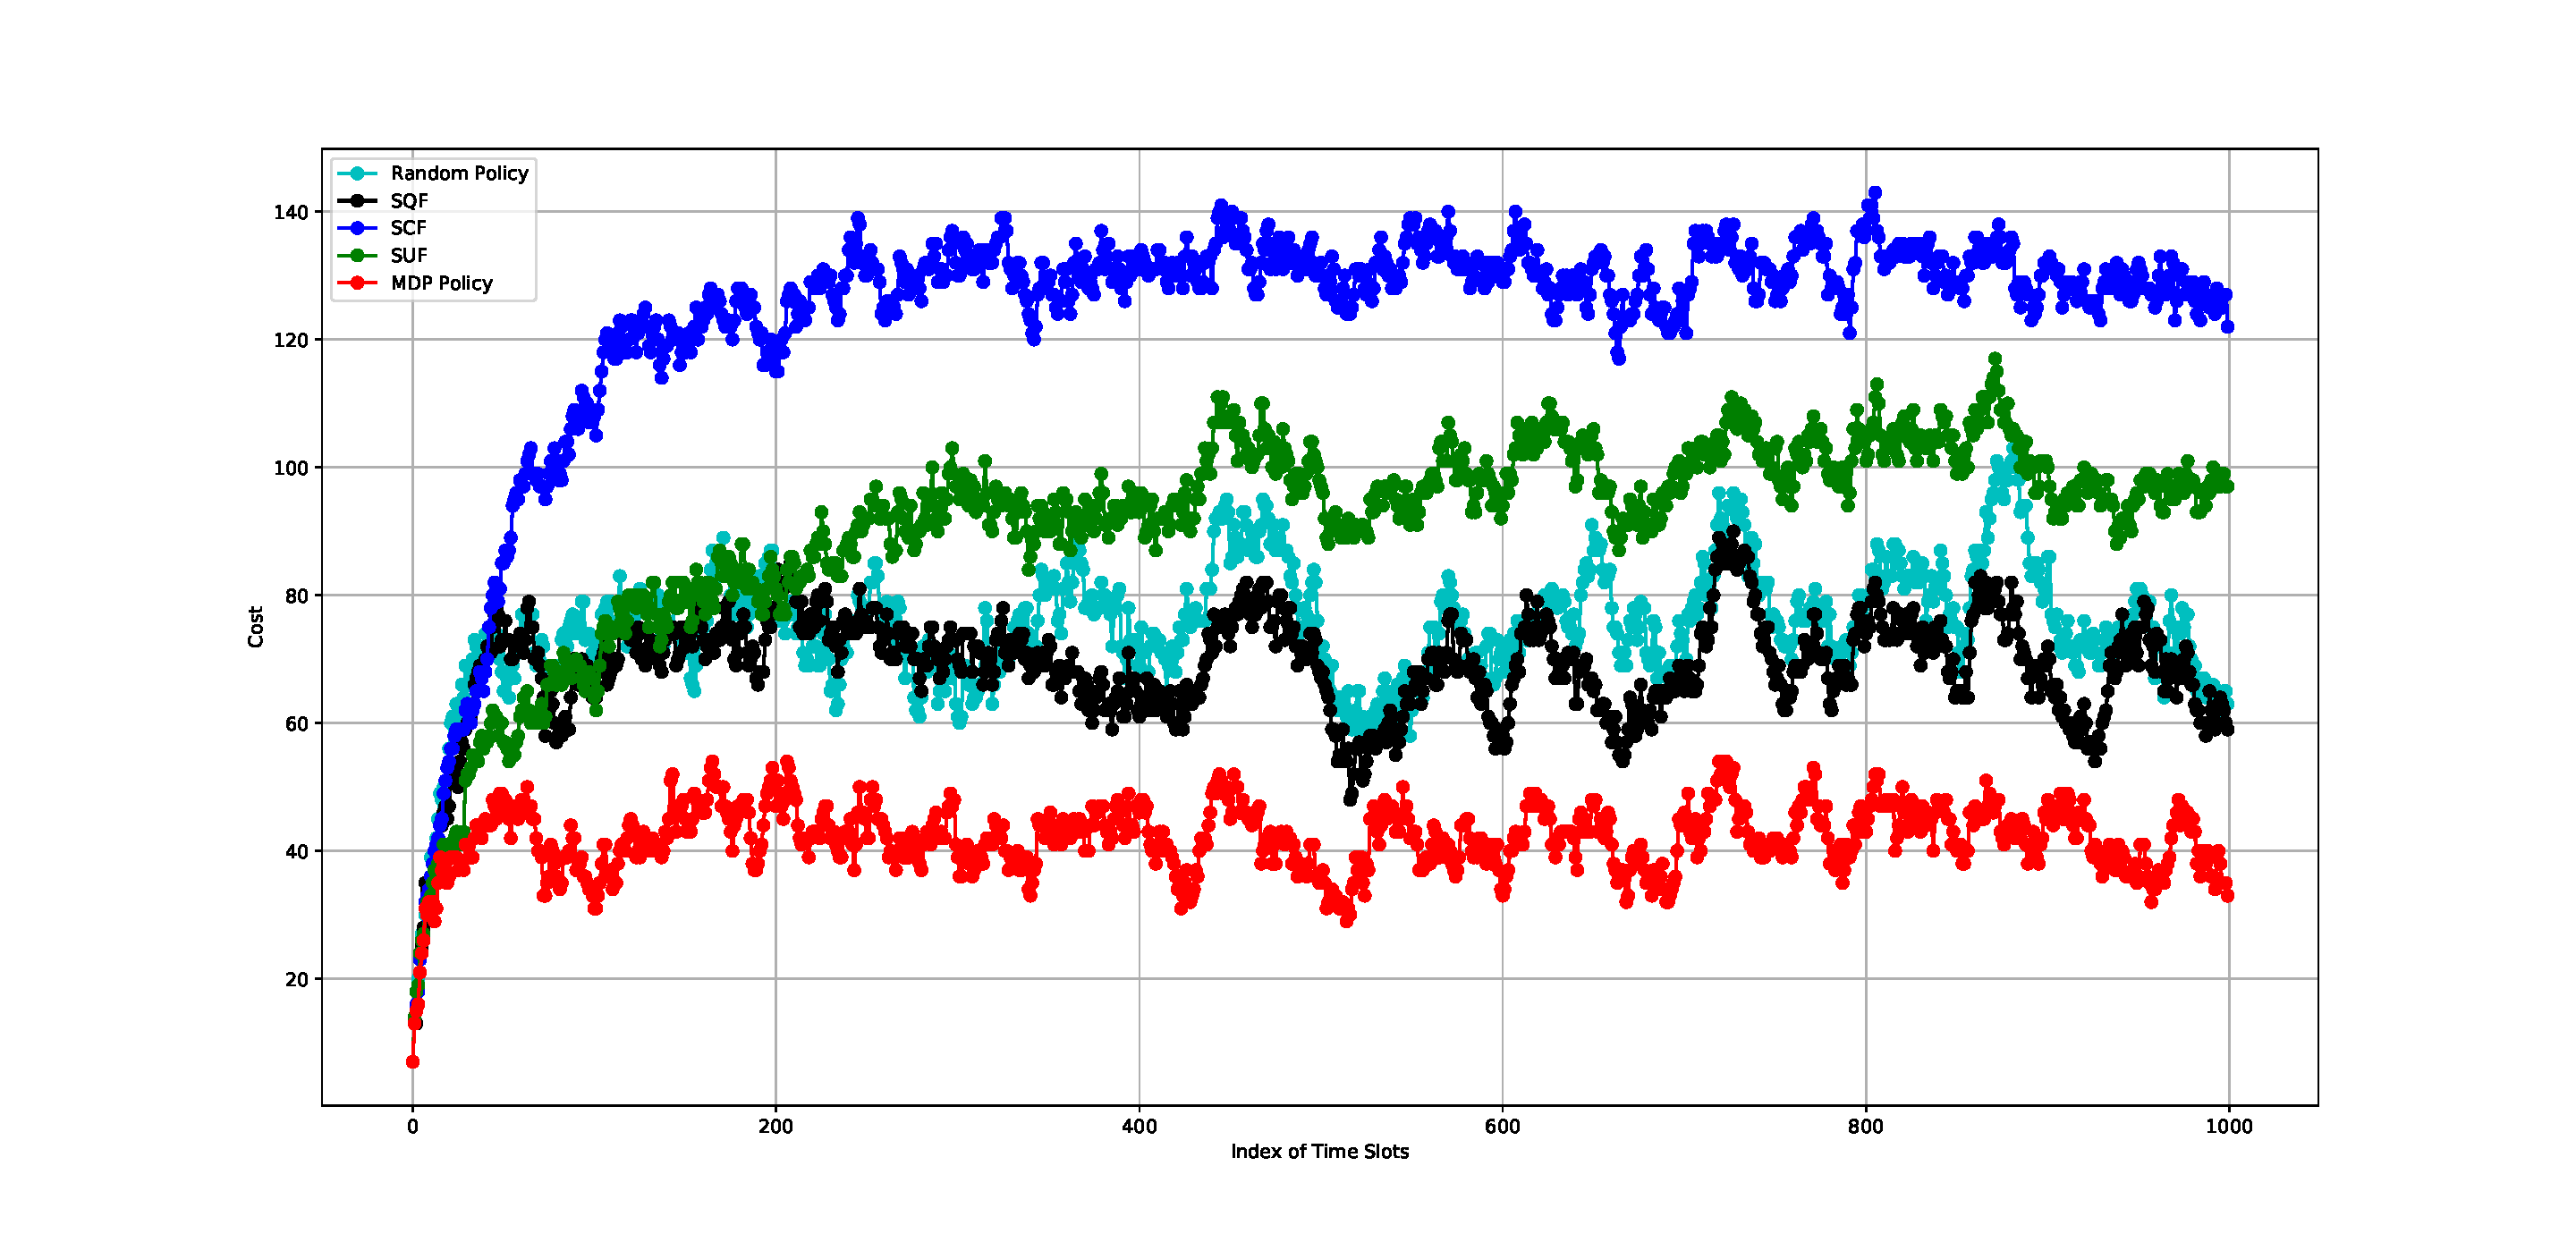
\includegraphics[width=1.0\textwidth]{chapter3_prev/timeline.pdf}
    \caption{The cost versus time slots when the average uploading delays and the job computation times are comparable. For example, the average uploading delay of the first job type from $1$-st AP to $1$-st edge server is $10$ time slots, and the job computation time of the first job type at the $1$-st edge server ranges from $10$ to $15$ time slots.}
    \label{fig:timeline}
\end{figure*}

\begin{figure*}
    \centering
    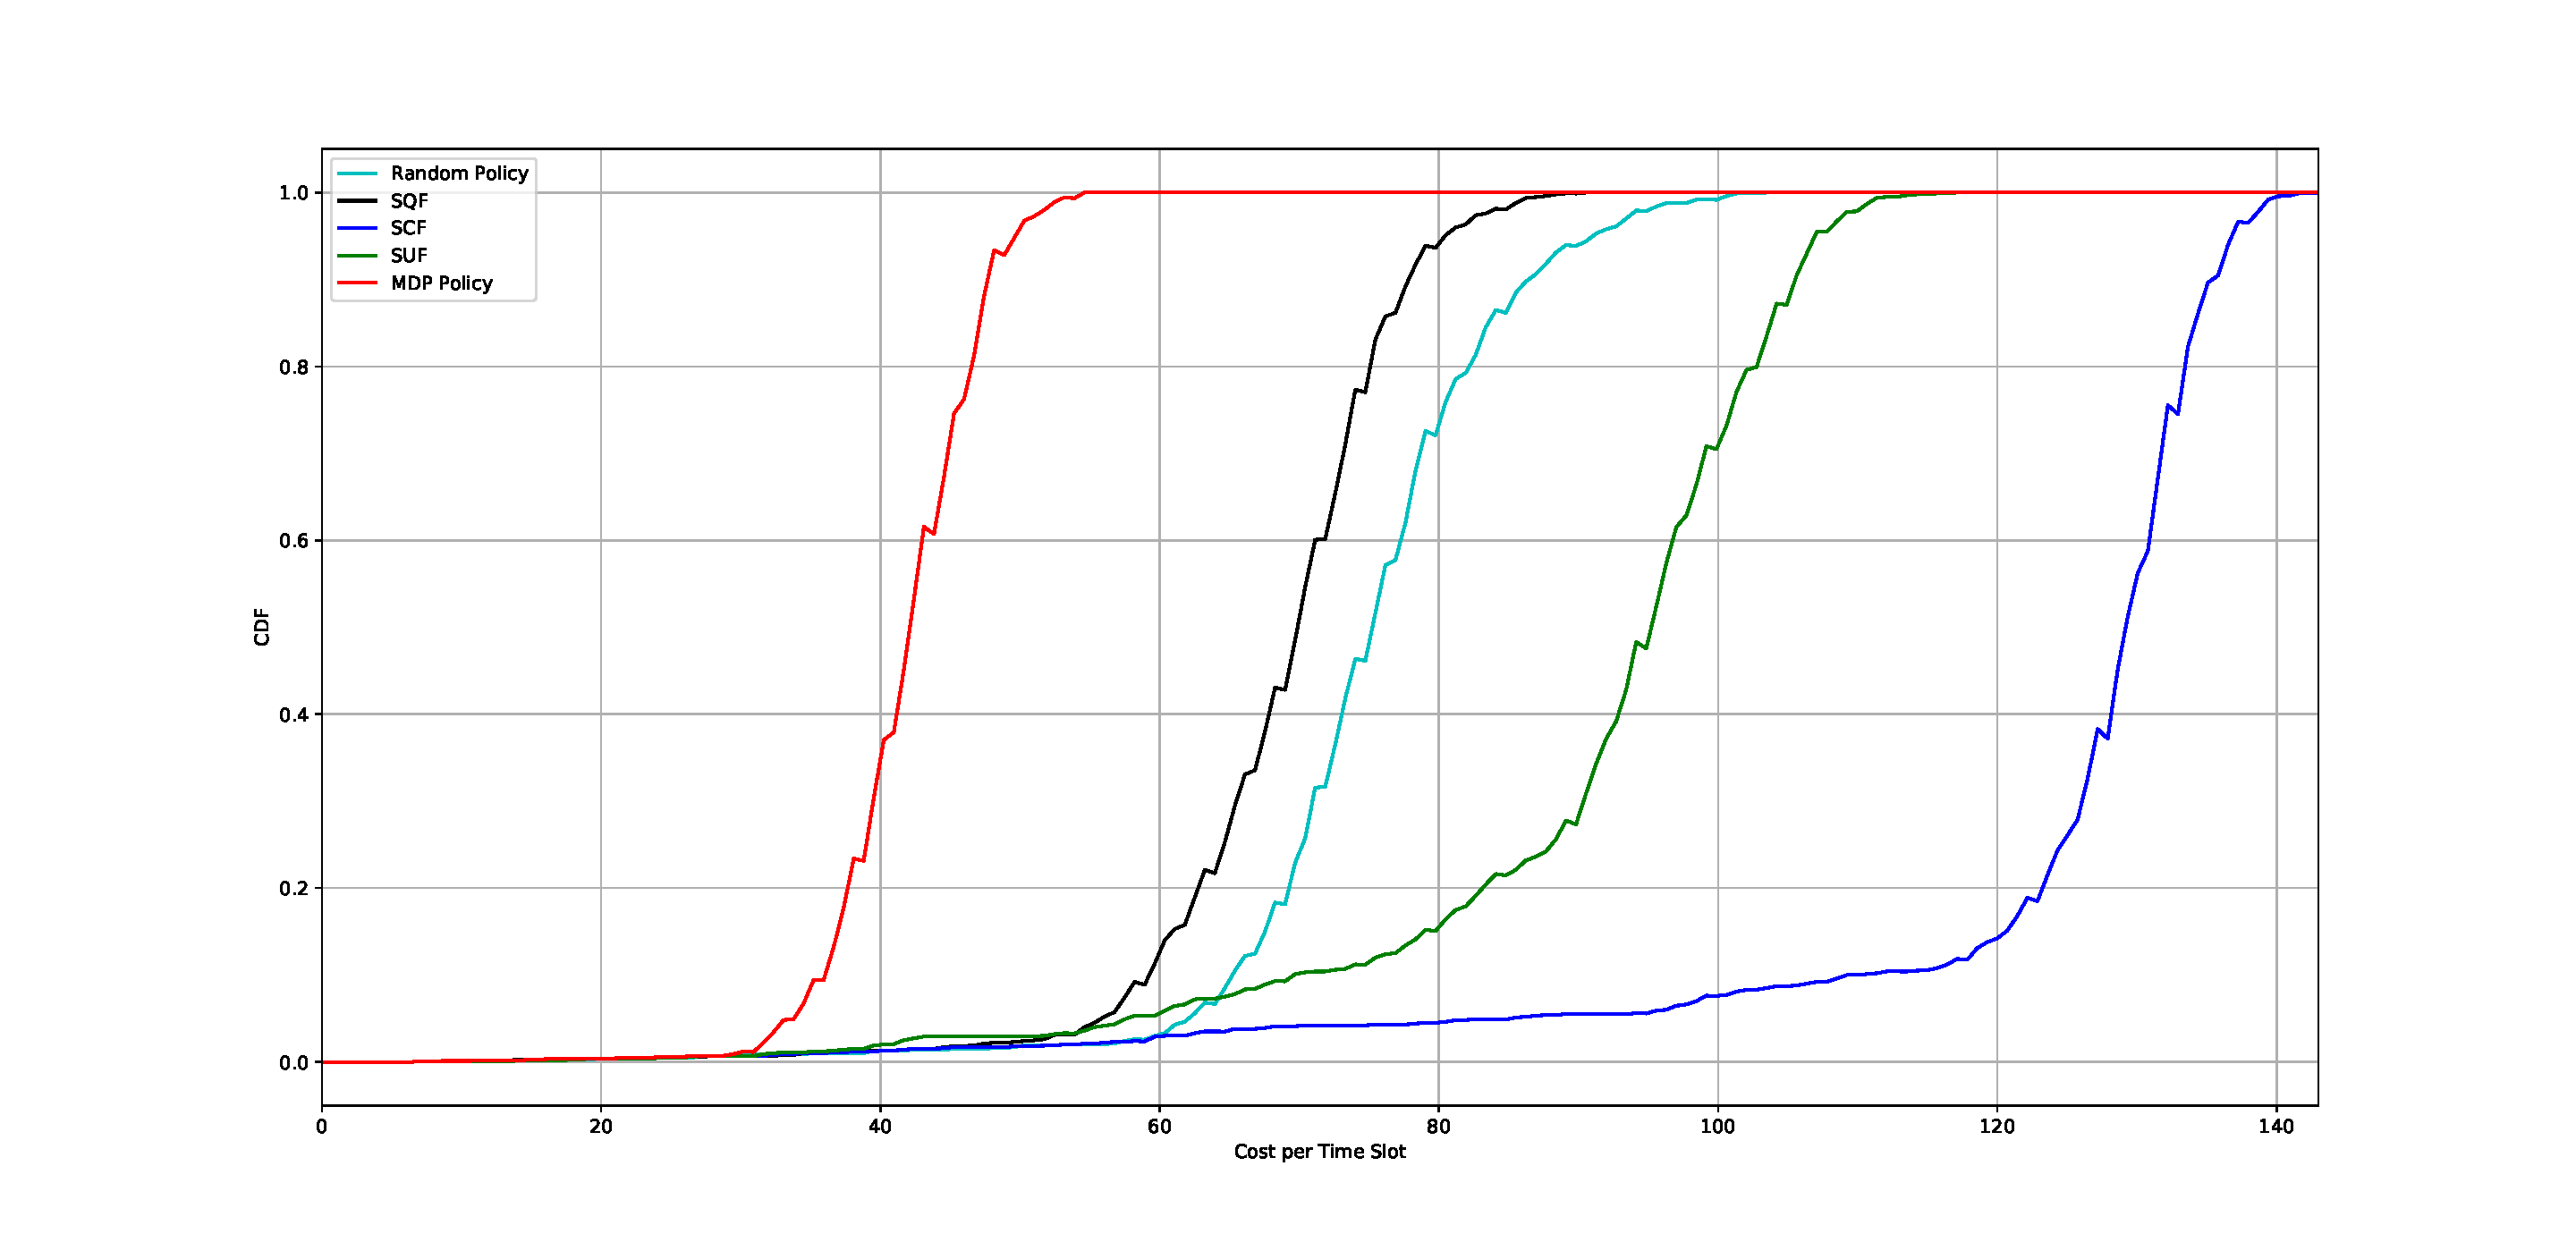
\includegraphics[width=1.0\textwidth]{chapter3_prev/general-setting.pdf}
    \caption{Cumulative distribution function(CDF) of the cost per time slot when average uploading delays and job computation times are comparable. For example, the average uploading delay of the first job type from first AP to first edge server is $10$ time slots, and the job computation time of the first job type at the first edge server ranges from $10$ to $15$ time slots.}
    \label{fig:cdf1}
\end{figure*}

In \figurename~\ref{fig:timeline} and \figurename~\ref{fig:cdf1}, the performance of the five schemes are compared when average uploading delays and job computation times are comparable. It can be observed that the proposed algorithm has significantly less cost per time slot than all the benchmarks. Note that in SQF algorithm, the job dispatching can be adjusted according to system state; whereas, the SUF and SCF algorithms have fixed job dispatching action in all the time slots. SQF algorithm has better performance than SUF and SCF algorithms.

\begin{figure*}
    \centering
    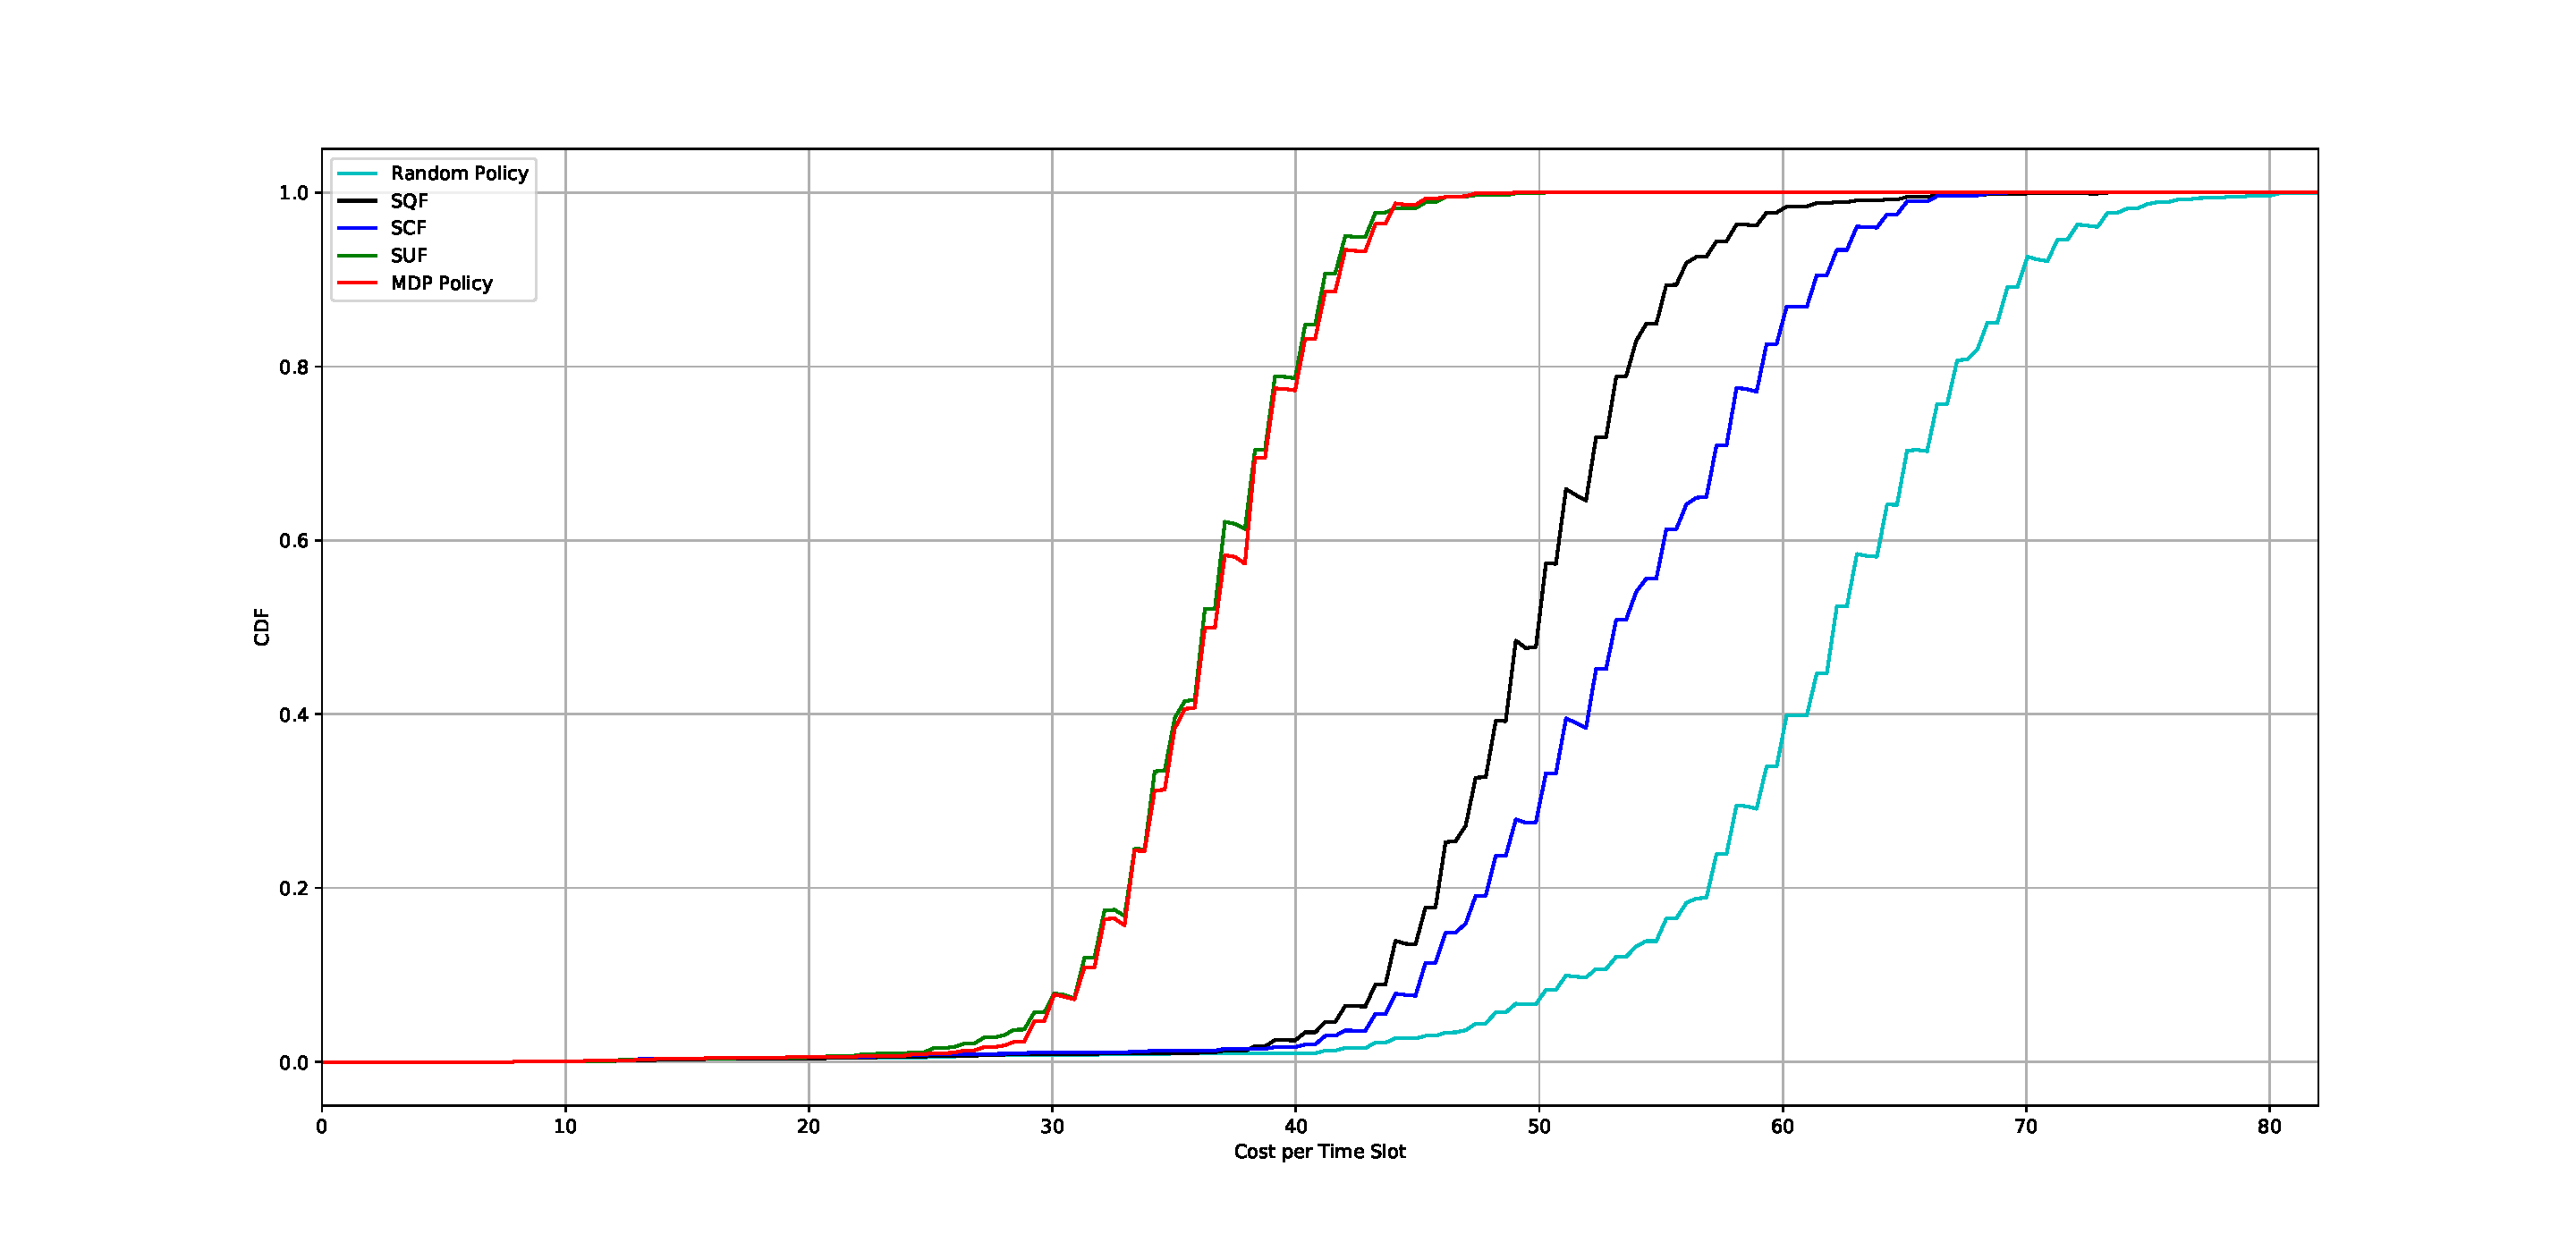
\includegraphics[width=1.0\textwidth]{chapter3_prev/only-ul.pdf}
    \caption{Cumulative distribution function (CDF) of the cost per time slot when average uploading delays are dominant. For example, the average uploading delay of the first job type from first AP to first edge server is $10$ time slots, and the average job computation time of the first job type at the first edge server is $1$ time slot.}
    \label{fig:cdf2}
\end{figure*}

In \figurename~\ref{fig:cdf2}, the average uploading delays are dominant, compared with the average job computation times. The performance of proposed algorithm is almost the same as the performance of SUF algorithm. Hence, in the edge computing network with dominant uploading delays, APs tend to dispatch the jobs to the edge server with shortest \emph{expected uploading time}.

\begin{figure*}
    \centering
    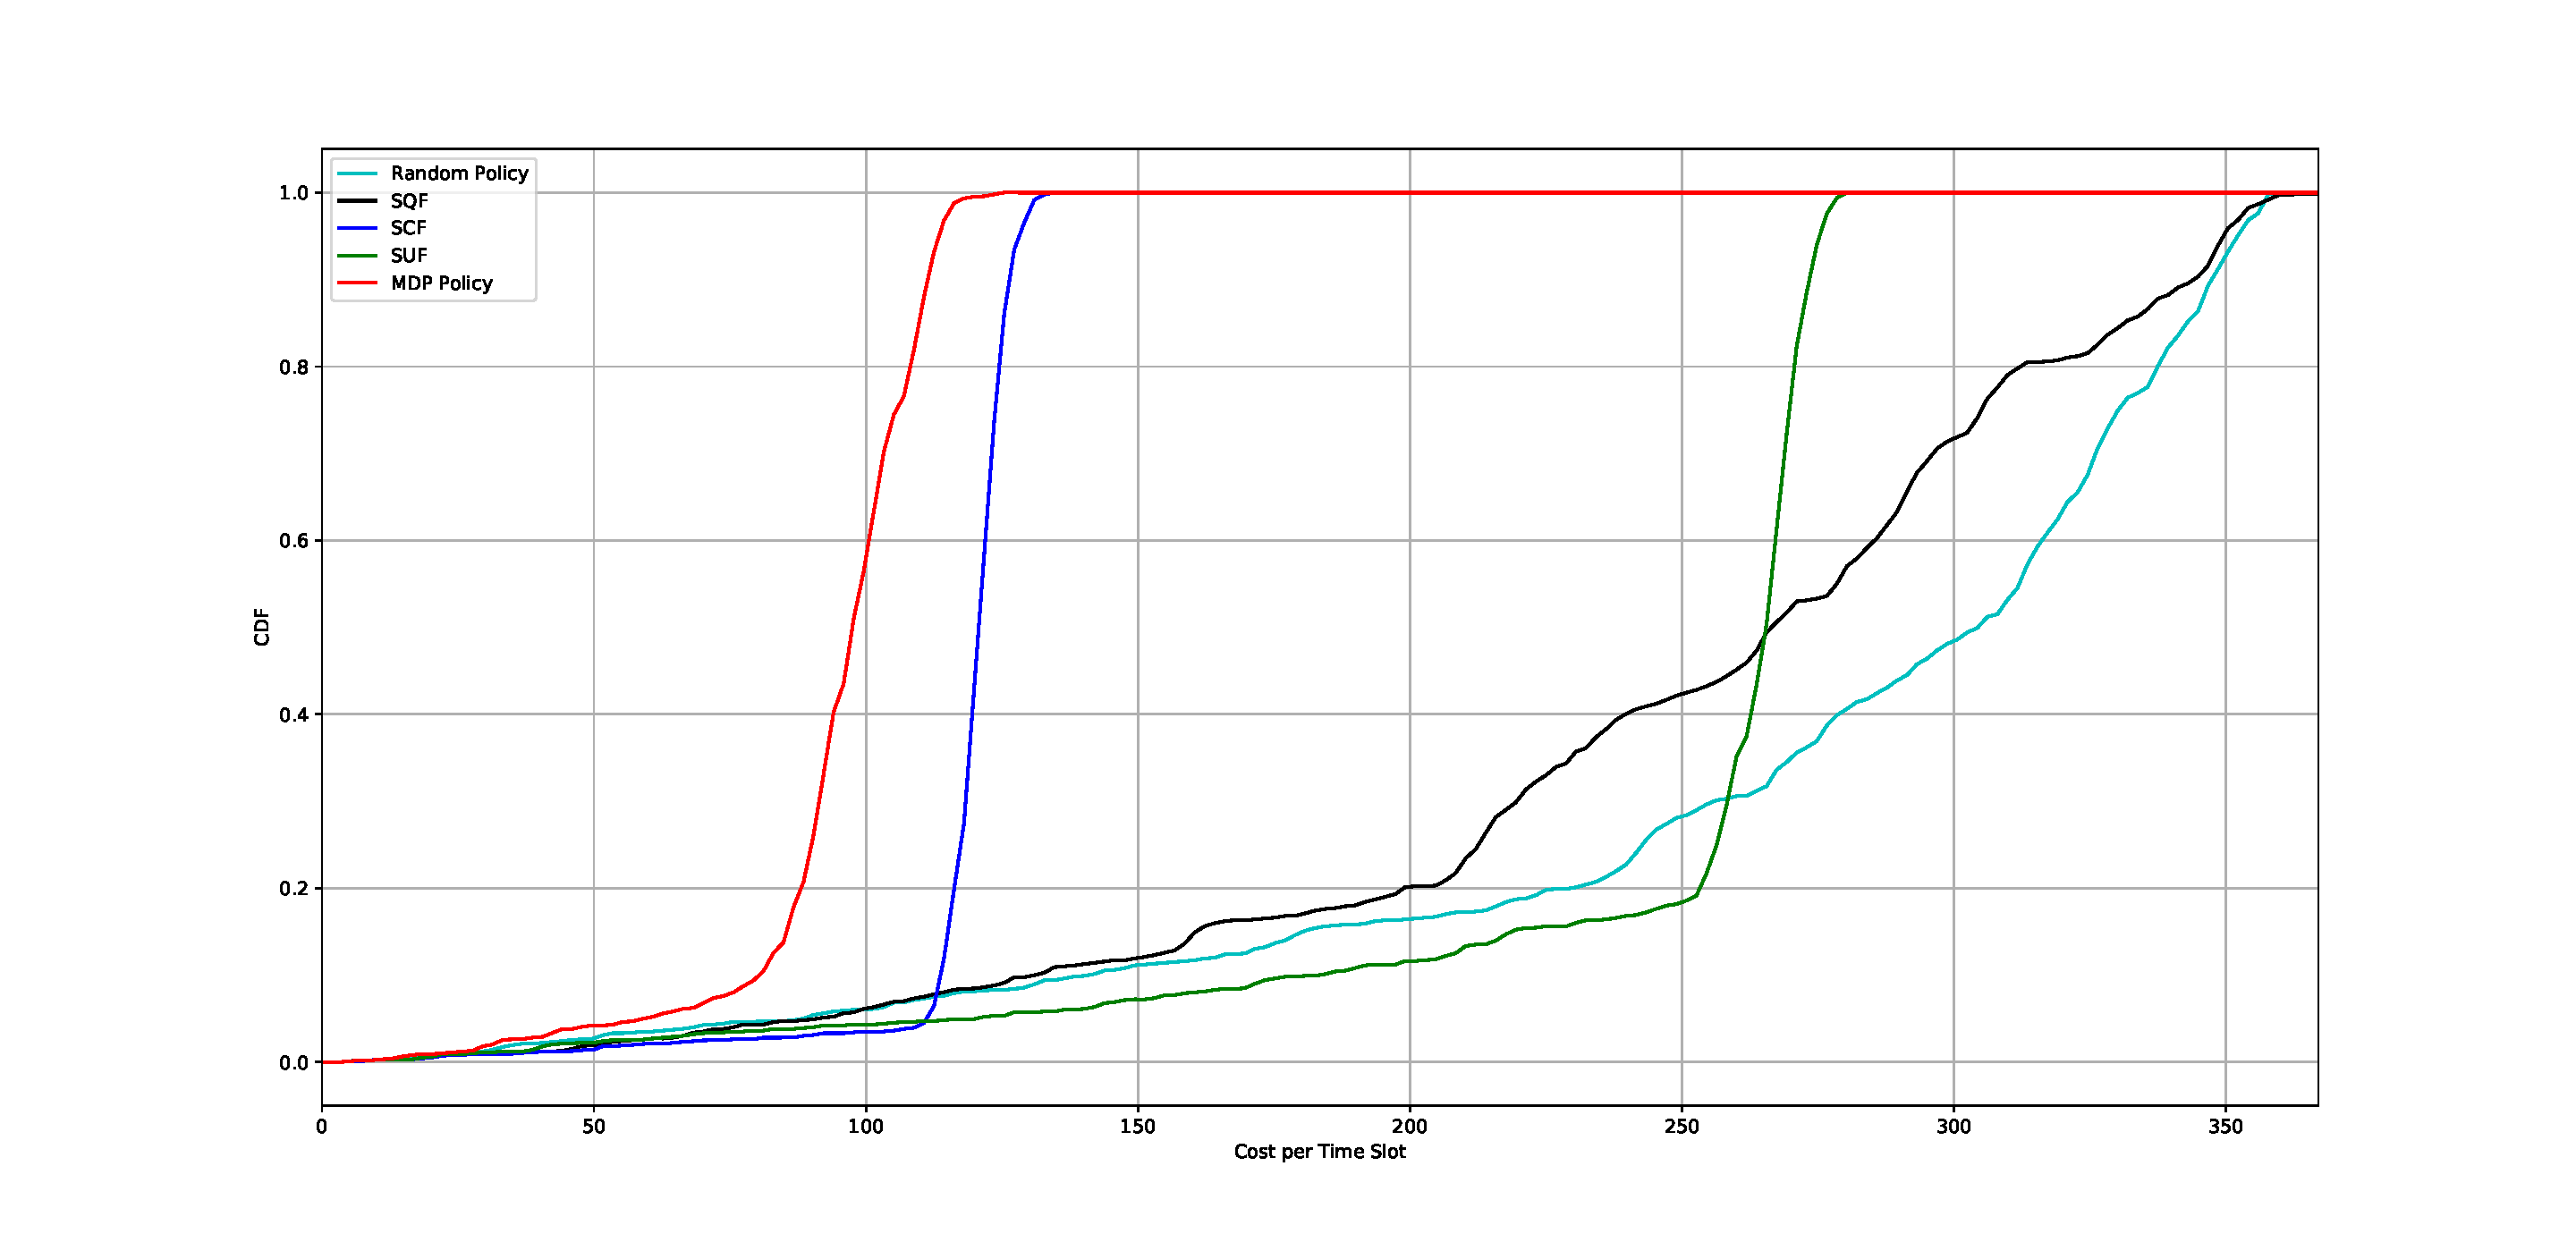
\includegraphics[width=1.0\textwidth]{chapter3_prev/only-computation-heavy.pdf}
    \caption{Cumulative distribution function (CDF) of the cost per time slot when average job computation times are dominant. For example, the average uploading delay of the first job type from first AP to first edge server is $1$ time slots, and the average job computation time of the first job type at the first edge server ranges from $10$ to $15$ time slots.}
    \label{fig:cdf3}
\end{figure*}

In \figurename~\ref{fig:cdf3}, the average job computation times are dominant, compared with the average uploading delays. It can be observed that the proposed algorithm has less cost per time slot than all the benchmarks. Note that SCF algorithm has better performance than other benchmarks, the APs tend to dispatch the jobs to the edge server with shortest \emph{expected computation time} in this situation.

\section{Summary}
\label{sec:chapter3_prev-conclusion}
In this chapter, we consider the cooperative job dispatching in an edge computing network with multiple APs and edge servers. The job uploading delay and computation time are both random and unpredictable. We formulate the joint optimization of job dispatching at all the APs and all the time slots as an infinite-horizon MDP with discounted cost. In order to avoid the curse of dimensionality, we also introduce a low-complexity sub-optimal solution based on one-step policy iteration from a baseline policy. The analytical performance bound is derived. Finally, it is shown by simulations that our proposed scheme has better performance than various benchmarks.
In Chapter 3, we shall extend the proposed algorithm to one new scenario where the delay of collecting complete system state information at each AP is not negligible.
Moreover, the memoryless distribution of uploading delay can also be generalized to arbitrary distribution.

        % !TeX root = ../../main.tex

\chapter{Distributed Job Dispatching in Edge Computing Networks with Random Transmission Latency: A Low-Complexity POMDP Approach}
\label{ch3}

In the previous chapter, we have investigated the centralized job dispatching problem in edge computing networks with random job arrivals, uploading latency and computation time.
In this Chapter, we extend the problem to a distributed job dispatching problem in edge computing networks with random signaling latency among edge servers.
The edge servers are deployed in closer proximity to mobile IoT devices than the traditional cloud computing infrastructure, which enable computation offloading from mobile IoT devices (e.g., mobile phones, video surveillance cameras, etc.) via Access Points (APs) and alleviate the communication overhead.
This brings new challenges to online job dispatching algorithm design, where the importance of cooperation among edge servers with outdated and partial signaling information is addressed.

%NOTE: (1b) why multiple edge servers deployed
Since the edge servers are usually with limited computation resources, the distributed deployment of edge computing servers in the network is favored.
Therefore, a fundamental problem in edge computing is to investigate the cooperative job dispatching among multiple APs and edge servers as illustrated in \figurename~\ref{fig:system}.
More specifically, mobile IoT devices offload jobs through APs, each of which performs as a job dispatcher to choose edge servers processing the data. Typically, there are a large number of APs in a Metropolitan Area Network (MAN). Some APs are co-located with edge servers while others are not.

\begin{figure*}[htp!]
    \centering
    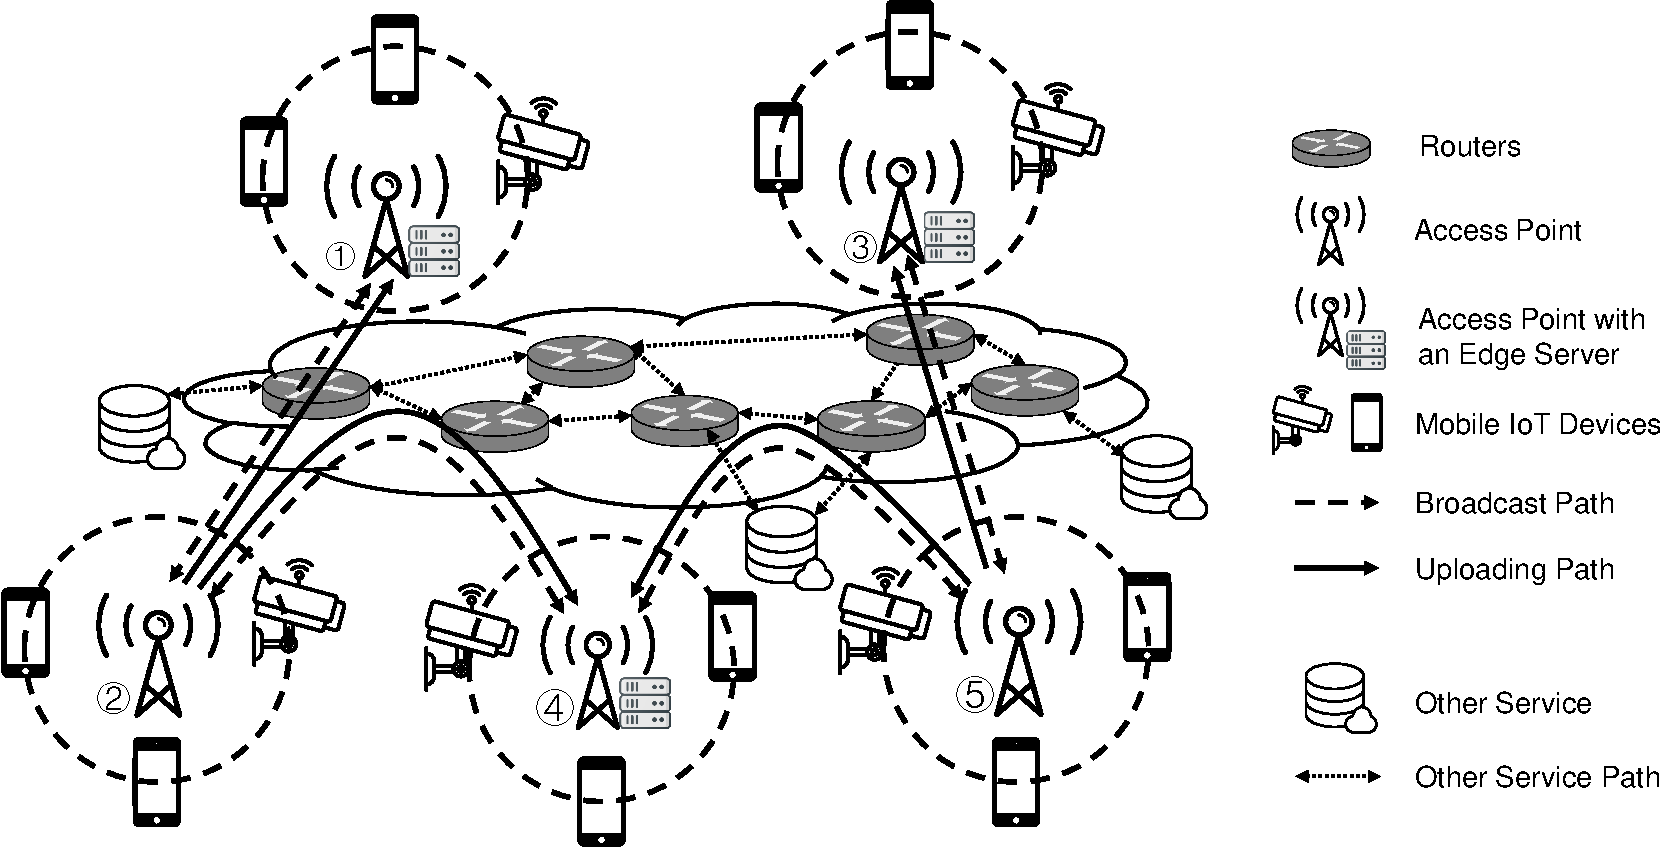
\includegraphics[width=1.0\textwidth]{chapter3/system-model.pdf}
    \caption{The illustration of system model.}
    \label{fig:system}
\end{figure*}

%NOTE: (2) Motivation with MAN and Distributed Dispatchers
%NOTE: (2a) why cooperation is needed; cooperation in MAN is another challenge
Most existing works assume a centralized job dispatcher, which has timely and complete knowledge of the global system status and distributes the dispatching decisions to all the APs without delay \cite{tan-online,IOTJ18-FanQ,mdp-globecom,mdp-tvt,MASS18-MengZ}.
However, the edge computing systems are usually deployed at Metropolitan Area Network (MAN) scale in practice, e.g., the Edge Computing Interconnect (ECI) Network \cite{MAN-ECI}, where the latency of information sharing among APs and edge servers is non-negligible. Moreover, according to the MAN performance analysis in \cite{MAN-LATENCY}, the end-to-end transmission latency is highly variable with respect to different hours of the day and IoT devices' locations in a MAN, which implies the randomness in the job uploading latency from APs to edge servers as well as the signaling latency (i.e., the transmission latency of the {system status} information).
%NOTE: (2b) challenge brought by random latency
There have been several works in the literature considering random transmission latency of job delivery in the edge computing network \cite{latency-EDGE19,MOBIHOC19-ZhouZ,IOTJ18-FanQ,TOC19-LiuC,JSAC19-AlameddineHA}.
However, there are few works considering the random signaling latency of information sharing among distributed dispatchers \cite{tan-online,TWC18-LyuX}.
In fact, it is full of {challenges} to consider random transmission latency in both job uploading and signaling in edge systems.
\begin{itemize}
    % 1) signaling latency: centralized/distributed, outdated information
    \item Firstly, the centralized dispatcher design is discouraged for unpredictable signaling latency, as the distribution of dispatching decisions would consume extra random time. For distributed dispatchers design, the information exchange among distributed dispatchers also suffers from significant signaling overhead and outdated information.
    % 2) uploading latency: inconsistency information exchange;
    \item Secondly, as the job arrivals at edge servers are unknown in advance because of random uploading latency, different dispatchers would have inconsistent system information even if the signaling latency is fixed.
\end{itemize}

To conclude, the random transmission latency may introduce ineliminable estimation errors on the number of jobs at APs or edge servers in the system.

% NOTE: (3) Our contributions
In this chapter, we address the above challenges by leveraging a partially observable Markov decision process (POMDP) problem formulation, and a novel low-complexity approximate MDP solution framework is proposed.
Specifically, we consider a practical scenario where the APs cooperatively upload different types of jobs to different edge servers with random uploading latency, and the APs receive the partial system state information suffering from random signaling latency (i.e., the global system state is always partially available and outdated at the APs).
The major contributions are summarized below.
\begin{itemize}
    \item The distributed and cooperative job dispatching design with outdated and partial information is formulated as a POMDP problem.
    Different from the conventional value or policy iteration of the Bellman's equations where global or historical system states are requested in numerical calculation, a novel low-complexity approximate MDP solution framework via \emph{alternative policy iteration} is proposed, where the dispatching policies of all APs are updated distributedly and alternatively based on the {closed-form expression} of the approximate local value function.
    Thus, the conventional complicated POMDP solution is avoided.
    \item Both analytical performance lower bound and tighter semi-analytical lower bound are derived for the proposed distributed dispatching policy. In the conventional approximate MDP methods, the performance is usually evaluated numerically.
    The lower bounds not only justify the reliability of the proposed policy but also provide a method of quick performance evaluation.
    \item We extend our solution framework {\Dalgname} with an efficient online learning approach to evaluate the approximate value function when the priori knowledge of the system randomness is absent.
    \item We conduct extensive simulations based on the Google Cluster trace, compared with three heuristic benchmarks. The evaluation results show that {\Dalgname} can achieve as high as $20.67\%$ reduction in average job response time and consistently perform well under various parameter settings of signaling latency, job arrival intensity and job processing time. {Moreover, the online learning algorithm converges fast.}
\end{itemize}

The remainder of this chapter is organized as follows.
In Section \ref{sec:chapter3-model}, we elaborate the system model and the signaling mechanism with random transmission latency.
In Section \ref{sec:chapter3-formulation}, we formulate the global-wise optimization of dispatching decisions at all APs as a POMDP.
In Section \ref{sec:chapter3-algorithm}, we propose a novel low-complexity approximate MDP solution framework, called {\Dalgname}.
% where the policy iteration could be applied distributedly on each AP {with partial and outdated information}.
In Section \ref{sec:chapter3-rl-alg}, the solution framework is extended with reinforcement learning technique to handle the unknown statistics.
The numerical analysis of the proposed solution is provided in Section \ref{sec:chapter3-evaluation}, and the conclusion is drawn in Section \ref{sec:chapter3-conclusion}.


%=================================================================================================%
%=================================================================================================%

\section{System Model}
\label{sec:chapter3-model}
In this section, we elaborate the model of edge computing networks with random job arrivals, uploading latency and computation time, as well as the signaling mechanism with periodic broadcast.
%----------------------------------------------------------------------------------------%
\subsection{Network Model}
We consider an edge computing system with $K$ Access Points (APs) and $M$ edge servers, which are connected in an edge network as illustrated in \figurename~\ref{fig:system}.
The sets of APs and edge servers are denoted as $\apSet \define \set{1,\dots,K}$ and $\esSet \define \set{1,\dots,M}$, respectively.
An edge server is typically deployed and collocated with an AP so that mobile devices can upload jobs efficiently.
The communication latency among these APs and edge servers is random.
Each AP collects the computation jobs from the {mobile IoT devices} within its coverage, and makes dispatching {decisions} on the edge servers for each job.
It is assumed that the $k$-th AP only dispatches the computation jobs to the edge servers within a certain number of hops.
Let $\esSet_{k} \subseteq \esSet$ be the subset of edge servers which can compute the jobs from the $k$-th AP, and $\apSet_{m}$ be the subset of APs, which may upload jobs to the $m$-th edge server.
We refer to $\esSet_{k}$ as the \emph{candidate server set} of the $k$-th AP, $\apSet_{m}$ as the \emph{potential AP set} of the $m$-th edge server, and $\rho_{k,m}$ as the collocation indicator (i.e., $\rho_{k,m}=1$ if $k$-th AP and $m$-th edge server collocated, otherwise $\rho_{k,m}=0$) ($\forall k\in\apSet, m\in\esSet$).

Different APs may have different candidate servers according to their locations in the network.
In this edge computing network, APs and edge servers periodically broadcast their state information (the state information is defined in Section \ref{subsec:chapter3-broadcast}), and one AP updates its strategy of job dispatching when receiving the broadcast state information.
We shall optimize the job dispatching strategy distributed at APs with partially observable state information, where both job uploading and state information broadcasting suffer from random transmission latency.

%NOTE: [job space support and arrival process]
Without loss of generality, it is assumed that there are $J$ types of jobs in this system, which are denoted via the set $\jSpace \define \set{1,\dots,J}$.
The time axis of dispatching is organized by time slots.
The arrivals of the type-$j$ jobs at the $k$-th AP ($\forall k\in\apSet,j\in\jSpace$) in different time slots are assumed to be independent and identically distributed (i.i.d.) Bernoulli random variables, and the arrival probability is denoted as $\lambda_{k,j}$.
Let $B_{k,j}(t) \in \set{0,1}$ represent the event of job arrival, where $B_{k,j}(t)=1$ means one type-$j$ job arrives at the $k$-th AP at the $t$-th time slot, and $B_{k,j}(t)=0$ means otherwise.
Hence,
\begin{align}
    \Pr\{ B_{k,j}(t) = 1 \} = \lambda_{k,j}, \forall t,k\in\apSet,j\in\jSpace.
\end{align}

%NOTE: [uploading process]
Each AP immediately dispatches each type of received jobs to one edge server.
As the APs upload jobs over shared edge networks illustrated in \figurename~\ref{fig:system}, the actual uploading time is random due to random traffics initiated from other enabled services.
Moreover, the notification of uploading completion from edge server to AP also consumes random time slots for the same reason, and thus the uploading time is unknown in advance.
Hence, we assume the uploading time of different types of jobs from different APs to edge servers follow independent and discrete distributions.
Let $\mathbb{U}_{k,m,j}(\Xi)$ be the uploading latency (in terms of time slots) distribution of the type-$j$ jobs from the $k$-th AP to the $m$-th edge server with support $\set{1, \dots, \Xi}$ ($\forall k\in\apSet, m\in\esSet, j\in\jSpace$), where $\Xi$ is the maximum possible uploading time for all jobs and the expectation is denoted as $u_{k,m,j}$.
Specifically, the uploading latency is fixed as $0$ if $\rho_{k,m}=1$ for job uploading to the collocated edge server.

%NOTE: [computation process]
For job computation process on edge servers, we adopt the \emph{unrelated machines assumption} as in \cite{tan-online} where the computation time on different edge servers would follow independent distributions.
Specifically, there are $J$ parallel virtual machines (VMs) running on each edge server for processing the $J$ job types, respectively.
It is assumed that the computation time of different job types on different edge servers follows independent memoryless geometric distribution 
\footnote{In this work, we adopt the memoryless geometric distribution to simplify the elaboration of algorithm. In fact, the proposed algorithm can be easily extended to other distributions.}
with different expectations as in \cite{TOWC18-HuangKb}.
Let $\mathbb{G}(1/c_{m,j})$ be the distribution of the computation time slots for the type-$j$ jobs on the $m$-th edge server, where $\mathbb{G}$ denotes the geometric distribution, $c_{m,j}$ is the expectation.
Let $f_{m,j}$ be its probability mass function (PMF), we have
\begin{align}
    f_{m,j}(x) \define (1-\frac{1}{c_{m,j}})^{x-1} \frac{1}{c_{m,j}}, x=1,2,\dots.
\end{align}
For each job type, the uploaded jobs are computed in a First-Come-First-Serve (FCFS) manner, and a processing queue with a maximum job number $L_{max}$ is established for each VM.
The arrival jobs will be discarded when the processing queue is full.

\begin{remark}[Generalization to Edge-Cloud Model]
    The above network model could be generalized into a computing system with both edge servers and cloud center.
    A cloud center could be treated as a special edge server in our model but with stronger computational capability and larger uploading latency and signaling latency to the APs.
\end{remark}

\subsection{Signaling Mechanism with Periodic Broadcast}
\label{subsec:chapter3-broadcast}
In order to facilitate distributed and cooperative dispatching for the APs, {the signaling mechanism with periodic broadcast is introduced.}
We refer to every $t_B$ time slots as a \emph{broadcast interval}.
As illustrated in \figurename~\ref{fig:brd_timeline}, at the beginning of each broadcast interval, the local state information (LSI) of APs and edge servers are broadcast, and each AP updates its dispatching strategy of job dispatching when observing the broadcast LSIs from some APs and edge servers.
As a remark notice that the observable LSI may be outdated due to transmission latency among APs and edge servers.
The LSI at the APs and edge servers, global state information, and observable state information at the APs are defined below, respectively.

%NOTE: State and Broadcast Information for AP
\begin{definition}[LSI of APs]
    Let $R^{(k)}_{m,j}(\xi,t,n) \in \set{0,1}$ be the indicator of the type-$j$ jobs at the $n$-th time slot of the $t$-th interval.
    Its value is $1$ when there is one job being uploaded from the $k$-th AP to the $m$-th server which has been delivered for $\xi$ time slots, and $0$ otherwise.
    Let $\omega_{k,j}(t)$ be the target edge server for the type-$j$ jobs of the $k$-th AP at the very beginning of the $t$-th broadcast interval.
    The LSI of the $k$-th AP at the beginning of the $t$-th broadcast interval is defined as
    \begin{align}
        \mathcal{R}_{k}(t) \define
        \Paren{
            \Brace{\vec{R}^{(k)}_{m,j}(t,0) \Big| \forall m\in\esSet,j\in\jSpace},
            \mathcal{A}_{k}(t)
        },
    \end{align}
    where
    \begin{align}
        \vec{R}^{(k)}_{m,j}(t,0) \define \Paren{
            R^{(k)}_{m,j}(0,t,0), \dots, R^{(k)}_{m,j}(\Xi,t,0)
        },
    \end{align}
    and
    \begin{align}
        \mathcal{A}_{k}(t) &\define \Brace{\omega_{k,j}(t) \Big| \forall j\in\jSpace}
    \end{align}
    are referred as status of the type-$j$ job uploading from the $k$-th AP to the $m$-th edge server, and the dispatching actions for all types of jobs of the $k$-th AP at the beginning of the $t$-th broadcast interval, respectively.
\end{definition}

%NOTE: State and Broadcast Information for Edge Server
\begin{definition}[LSI of Edge Servers]
    Let $Q_{m,j}({t,n})$ be the number of type-$j$ jobs on the $m$-th edge server at the $n$-th time slot of the $t$-th interval ($\forall m\in\esSet, j\in\jSpace$).
    The LSI of the $m$-th edge server at the $t$-th broadcast interval is defined as
    \begin{align}
        \mathcal{Q}_{m}(t) \define \Brace{
            Q_{m,j}(t, 0) \Big| \forall j\in\jSpace
        }.
    \end{align}
\end{definition}

\begin{definition}[Global State Information]
    The global state information (GSI) of the $t$-th broadcast interval is defined as the aggregation of the broadcast LSIs from all the APs and edge servers, i.e.,
    \begin{align}
        \Stat(t) \define
            \Paren{
                \Brace{\mathcal{R}_{k}(t) \Big| \forall k\in\apSet},
                \Brace{\mathcal{Q}_{m}(t) \Big| \forall m\in\esSet}
            }.
    \end{align}
\end{definition}

%NOTE: Conflict of AP set and partial information definition
As the APs and edge servers may reside in different locations of a MAN, the transmission latency of LSI is not negligible.
It might be inefficient {and costly} for one AP to collect the complete GSI before the update of dispatching policy.
For example, the transmission latency of the LSI from the edge servers outside the \emph{candidate server set} $\esSet_{k}$ to the $k$-th AP may be large, and some broadcast information may be discarded by the routers after a certain number of hops.
In this chapter, we shall investigate the distributed dispatching design based on the \emph{observable state information} at each AP.
Specifically, the \emph{conflict AP sets} and the \emph{observable state information} are defined below, respectively.
\begin{definition}[Conflict AP Set]
    The conflict AP set to the $k$-th AP ($\forall k\in\apSet$) consists of the neighboring APs who share any common edge server with the $k$-th AP, i.e.,
    \begin{align}
        \ccSet_{k} \define \bigcup_{m\in\esSet_{k}} \apSet_{m}.
    \end{align}
\end{definition}

\begin{definition}[Observable State Information]
    \label{def:OSI}
    The observable state information (OSI) of the $k$-th AP ($\forall k\in\apSet$) at the $t$-th broadcast interval is defined as the aggregation of LSIs of the APs in {conflict AP set} and the edge servers in {candidate server set} of the $k$-th AP, i.e.,
    \begin{align}
        \Stat_{k}(t) &\define
        \Paren{
            \Brace{\mathcal{R}_{k'}(t) \Big| \forall k'\in\ccSet_{k}},
            \Brace{\mathcal{Q}_{m}(t) \Big| \forall m\in\esSet_{k}}
        }.
    \end{align}
\end{definition}

\begin{figure*}[t]
    \centering
    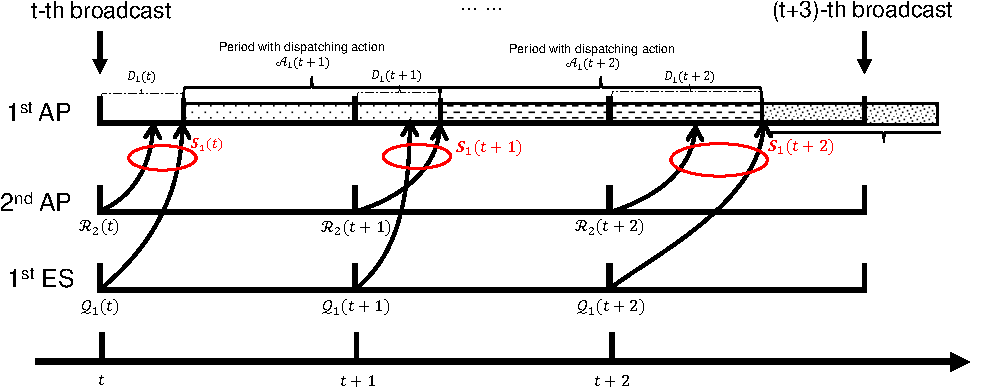
\includegraphics[width=1.0\textwidth]{chapter3/brd-timeline.pdf}
    \caption{The timeline illustration of reception of OSI for the $1$-st AP where $2$-nd AP is in its \emph{conflict AP set} and $1$-st server is in its \emph{candidate server set}.}
    \label{fig:brd_timeline}
\end{figure*}

The $k$-th AP is able to collect its OSI $\Stat_{k}(t)$ at the $\mathcal{D}_{k}(t)$-th time slots of the $t$-th broadcast interval, where the {\emph{\brlatency}} $\mathcal{D}_{k}(t)$ is a random variable.
It is assumed that $\mathcal{D}_{k}(t)$ follows identical and independent distribution in different broadcast interval.
An example is given below to demonstrate how the {\brlatency} affects the reception of OSI and the update of the dispatching strategy.
Moreover, the notations used throughout this chapter are summarized as in Table \ref{table:symbols}.

\begin{example}
    In \figurename~\ref{fig:brd_timeline}, the $2$-nd AP and $1$-st server are in the \emph{conflict AP set} and \emph{candidate server set} of the $1$-st AP, respectively.
    At the beginning of the $t$-th broadcast interval, the dispatching actions $\mathcal{A}_{1}(t)$ is adopted by the $1$-st AP.
    After $\mathcal{D}_{1}(t)$ time slots, it updates the dispatching actions to $\mathcal{A}_{1}(t+1)$ based on its OSI $\Stat_{1}(t)$.
    In the $(t+1)$-th broadcast interval, the $1$-st AP will firstly keep the previous actions $\mathcal{A}_{1}(t+1)$, and then updates the actions $\mathcal{D}_{1}(t+1)$ time slots later based on $\Stat_{1}(t+1)$. The new action is denoted as $\mathcal{A}_{1}(t+2)$.
    The signaling latency $\mathcal{D}_1(t)$ and $\mathcal{D}_1(t+1)$ can be different.
\end{example}

\begin{remark}[Transmission Failure of OSI]
    % [Handling Broadcast Information Transmission Failure]
    % R1-1: How do you deal with the failed transmission of system state information?
    % R2-2: What if the information broadcast by the 2-nd AP is not received by the 1-st AP?
    In the system model, the transmission failure of OSI is tolerable: it can actually be transferred to transmission latency.
    For example, if the $y$-th AP is in the \emph{conflict AP set} of the $k$-th AP and the state information transmission from the $y$-th AP failed, the $k$-th AP may request retransmissions until a successful reception.
    This will raise the transmission latency of OSI, which contributes to the random {\brlatency} $\Delay_{k}(t)$ of the $k$-th AP.
\end{remark}

\begin{table}[htp!]
    \footnotesize
    \centering
    \caption{Table of notations and their descriptions throughout this chapter.}
    \label{table:symbols}
    \begin{tabulary}{1.0\linewidth}{|p{2.5cm}|L|}
        \hline
        Notation                        & Description \\
        \hline
        $\mathcal{K}$                   & The denotation of AP set \\
        $\mathcal{M}$                   & The denotation of edge server set \\
        $\mathcal{K}_{m}$               & The potential AP set of the $m$-th edge server \\
        $\mathcal{M}_{k}$               & The candidate edge server set of the $k$-th AP \\
        $\ccSet_{k}$                    & The conflict AP set of the $k$-th AP  \\
        $\mathcal{J}$                   & The denotation of job types set \\
        $\lambda_{k,j}$                 & The average arrival job rate for the type-$j$ job on the $k$-th AP \\
        $c_{m,j}$                       & The average computation time for the type-$j$ job on the $m$-th edge server \\
        $L_{max}$                       & The maximum job number for each VM \\
        $t_B$                           & The duration of a broadcast interval \\
        $\Xi$                           & The maximum job uploading time \\
        $\xi$                           & The index of time slot of uploading time for one job \\
        $\mathbb{U}_{k,m,j}(\Xi)$       & The uploading latency distribution of the type-$j$ jobs from the $k$-th AP to the $m$-th edge server \\
        $\mathcal{R}_{k}(t)$            & The LSI of the $k$-th AP at the beginning of the $t$-th broadcast interval \\
        $\mathcal{Q}_{m}(t)$            & The LSI of the $m$-th edge server at the beginning of the $t$-th broadcast interval \\
        $D_{k}(t)$                      & The {\brlatency} for the $k$-th AP at the $t$-th broadcast interval \\
        $\mathbb{D}(t)$                 & The vector of all {\brlatency} at the $t$-th broadcast interval \\
        $\Stat(t)$                      & The GSI at the $t$-th broadcast interval \\
        $\Stat_{k}(t)$                  & The OSI of the $k$-th AP at the $t$-th broadcast interval \\
        $\omega_{k,j}(t)$               & The dispatching action for type-$j$ job on the $k$-th AP at the beginning of $t$-th broadcast interval \\
        $\mathcal{A}_{k}(t)$               & The dispatching actions of the $k$-th AP at the beginning of $t$-th broadcast interval \\
        $\Policy(\Stat(t),\Delay(t))$   & The aggregation of individual policy all APs \\
        $\Baseline(\Stat(t),\Delay(t))$ & The proposed baseline policy \\
        $\gamma$                        & The discount factor \\
        $\beta$                         & The weight of overflow penalty \\
        $\mathcal{Y}_{n}$               & The $n$-th subset partition in which the APs update their dispatching actions parallel \\
        $\tilde{\mathcal{A}}(t)$        & The aggregation of dispatching actions of the APs in the subset $\mathcal{Y}_{n}$, where $n \define t \pmod{N}$  \\
        $\hat{\mathcal{A}}(t)$          & The aggregation of dispatching actions of the APs not in the subset $\mathcal{Y}_{n}$, where $n \define t \pmod{N}$ \\
        \hline
    \end{tabulary}
\end{table}

%=================================================================================================%
%=================================================================================================%

\section{POMDP-based Problem Formulation}
\label{sec:chapter3-formulation}
%----------------------------------------------------------------------------------------%
In this section, we formulate the optimization of job dispatching problem of all APs as a Markov decision process (MDP).
Since each AP updates the job dispatching action according to OSI instead of GSI, the MDP problem is a partially observable MDP (POMDP).
Firstly, we give the definitions of \emph{dispatching policy} and \emph{cost function}, together with the \emph{system state} (i.e., the GSI) defined previously, to complete the MDP problem formulation.

\begin{definition}[Dispatching Policy]
    The individual dispatching policy of the $k$-th AP, denoted as $\Omega_{k}$ ($\forall k \in\apSet$), maps from its OSI $\Stat_{k}$ and its {\brlatency} $\mathcal{D}_{k}$ to the dispatching action for each job type, i.e.,
    \begin{align}
        \Omega_{k} \Paren{ \Stat_{k}(t), \mathcal{D}_{k}(t) }
        &\define \mathcal{A}_{k}(t+1)
        \nonumber\\
        &= \Brace{
            \omega_{k,j}(t+1) \Big| \forall j\in\jSpace
        }.
        \label{def:action}
    \end{align}

    The aggregation of individual policy of all APs is referred to as the system dispatching policy $\Policy$.
    Thus,
    \begin{align}
        \Policy\Paren{ \Stat(t), \Delay(t) } \define \Brace{
            \Omega_{1}(\Stat_{1}(t), \mathcal{D}_{1}(t)), \dots, \Omega_{K}(\Stat_{K}(t),\mathcal{D}_{K}(t))
        },
    \end{align}
    where $\Delay(t) \define \set{ \mathcal{D}_{1}(t), \dots, \mathcal{D}_{K}(t) }$.
\end{definition}

The average job response time and packet drop rate are considered as the system cost.
The job response time counts the number of broadcast intervals from job arrival to the accomplishment of computation, which includes the uploading time from the AP to the edge server, the waiting time in the processing queue and the job processing time on the edge server.
According to the Little's law \cite{Little1961}, the average response time per job, counting the number of broadcast intervals from job arrival to the accomplishment of computation, is proportional to the number of jobs in the system, given the job arrival rates at all the APs.
Hence, we define the cost function per broadcast interval as follows, {given the information contained in periodic broadcast.}

\begin{definition}[Cost Function per Broadcast Interval]
    The cost function of the $t$-th broadcast interval with GSI $\Stat(t)$ is defined as
    \begin{align}
        g\Paren{\Stat(t)} \define
            \sum_{m\in\esSet,j\in\jSpace}
            \Brace{&
                \sum_{k\in\apSet} \Inorm{\vec{R}^{(k)}_{m,j}(t,0)} + Q_{m,j}(t,0)
                + \beta \cdot I[Q_{m,j}(t,0)=L_{max}]
            },
    \end{align}
    where $\Inorm{\vec{x}}$ denotes the $L^1$-norm of the vector $\vec{x}$, $\sum_{k\in\apSet} \Inorm{\vec{R}^{(k)}_{m,j}(t,0)}$ measures the number of type-$j$ jobs being uploaded from the $k$-th AP to the $m$-th edge server, $Q_{m,j}(t,0)$ measures the number of type-$j$ jobs on the $m$-th edge server, and $\beta$ is the weight of overflow penalty.
    The cost function per broadcast interval could be taken as a uniform sampling of cost function per time slot.
\end{definition}

Since the job dispatching in one broadcast interval will affect the GSI of the following broadcast intervals, we should consider the joint minimization of the costs of all the broadcast intervals.
Specifically, we consider the following discounted sum of the costs of all the broadcast intervals as the system objective.
\begin{align}
    &\bar{G}(\Stat(1), \Policy) \define
    \lim_{T \to \infty} \mathbb{E}^{\Policy}_{\set{\Stat(t)|\forall t}, \Delay}
    \Bracket{
        \sum_{t=1}^{T} \gamma^{t-1} g\Paren{\Stat(t)} \Big| \Stat(1)
    },
\end{align}
where $\mathbb{E}^{\Policy}_{\set{\Stat(t)|\forall t}}[\cdot]$ denotes the expectation with respect to all possible system states in the future given scheduling policy $\Policy$, and $\gamma \in (0,1)$ is the discount factor.
Hence, the optimization of job dispatching policy can be formulated as the following minimization problem.
\begin{align}
    \textbf{P1:}~
    \min_{\Policy} \bar{G}(\Stat(1), \Policy).
\end{align}

If the GSI $\Stat(t)$ and {\brlatency} $\Delay(t)$ are known to all the APs, the MDP in problem P1 can be solved via the following Bellman's equations as in \cite{sutton1998}.
\begin{align}
    V\Paren{\Stat(t)} =&g\Paren{\Stat(t)}
        + \gamma\mathbb{E}_{\Delay}\bigg\{
            \min_{\Policy(\Stat(t),\Delay(t))}
            \nonumber\\
            &\sum_{\Stat(t+1)} \Pr \Big\{ 
                \Stat(t+1) \Big| \Stat(t), \Policy(\Stat(t), \Delay(t)) \Big\} \cdot V\Big(\Stat(t+1)\Big)
            \bigg\},
    \label{eqn:sp_0}
\end{align}
where the value function $V(\Stat(t))$ of the optimal policy $\Policy^{*}$ (if GSI and {\brlatency} are known to all the APs) is defined as follows.
\begin{align}
    &V\Paren{\Stat(t)} \define
    \lim_{T\to\infty} 
    \mathbb{E}^{\Policy^*}_{\set{\Stat(t)|\forall t}, \Delay} \Bracket{
        \sum_{t=1}^{T} \gamma^{t-1} g\Big( \Stat(t) \Big) \Big| \Stat(1)
    }.
    \label{eqn:val_f}
\end{align}
Moreover, the optimal dispatching policy $\Omega^{*}$ can be obtained by solving the right-hand-side (RHS) of the above Bellman's equations (\ref{eqn:sp_0}).

However, it is infeasible to solve the above Bellman's equations {and achieve the performance of $\Policy^*$ in our considered distributed dispatching scenario.}
This is because each AP (say the $k$-th AP) only has the knowledge of its own OSI $\Stat_{k}(t)$ and local {\brlatency} $\mathcal{D}_{k}(t)$, but the optimal solution (dispatching actions of all APs) for the RHS of Equation (\ref{eqn:sp_0}) depends on the GSI and the knowledge of global {\brlatency}.
Thus, problem P1 is actually a POMDP, which is further demonstrated by a toy example below.

\begin{figure*}[htp!]
    \centering
    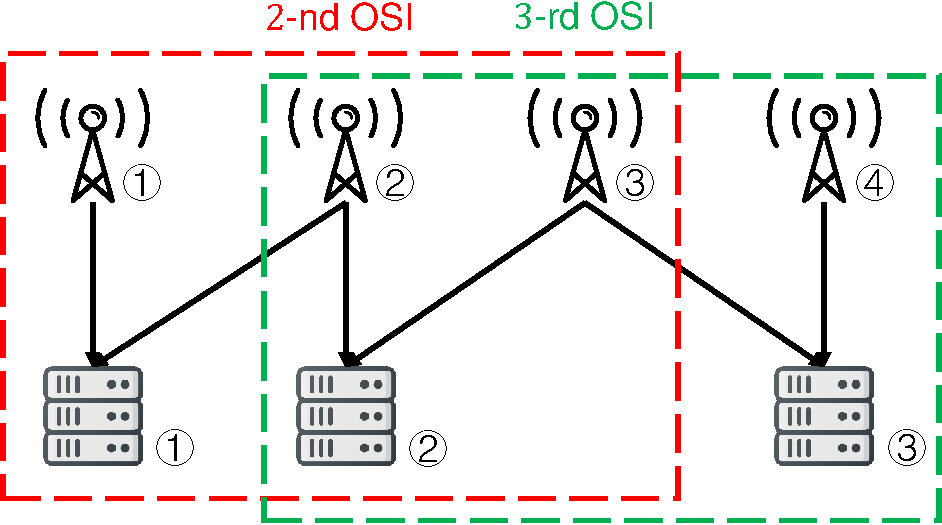
\includegraphics[width=1.0\textwidth]{chapter3/osi-example.pdf}
    \caption{An example of system model, where the edge servers $1,2,3$ are collocated with the APs $1,2,4$, respectively.}
    \label{fig:osi_example}
\end{figure*}

\begin{example}
    As illustrated in \figurename~\ref{fig:osi_example}, there are four APs and three edge servers collocated with the APs, in the edge computing system, where the solid directed lines show all the possible job dispatching paths for the APs.
    For the $2$-nd AP, its OSI includes the state information of the APs indexed with $1,3$ and the edge servers indexed with $1,2$.
    The state information of the $3$-rd edge server is out of its scope.
    
    Moreover, the OSI of the $3$-rd AP (namely, the $3$-rd OSI) includes the state information of the APs indexed with $2,4$ and the edge servers indexed with $2,3$.
    Note that the prediction of future state distribution is essential for solving the RHS of Equation (\ref{eqn:sp_0}).
    Without GSI, it is impossible to predict the future dispatching decisions of the $3$-rd AP from the perspective of the $2$-nd AP, since they observe different OSIs.
    It is thereby impossible for the $2$-nd AP to predict the future state distributions of the $2$-nd edge server, lack of the dispatching decisions of the $3$-rd AP.
    As a result, the evaluation of optimal value function of Equation (\ref{eqn:val_f}) is infeasible at both $2$-nd and $3$-rd APs, and the distributed policy optimization for them is a POMDP.
\end{example}

The general solution of POMDP is of huge complexity {as all the historical system states should be traced back in the current system state} \cite{IJCAI03-NairR,IJCAI99-BoutilierC}.
In this chapter, we shall propose a novel low-complexity solution framework based on an analytical approximation of the value function $V(\cdot)$ and alternative actions update, where distributed job dispatching via the Bellman's equations becomes feasible
(the minimization at the RHS of Equation (\ref{eqn:sp_0}) is solvable with the approximate value function)
even with OSI and local {\brlatency}.

%=================================================================================================%
%=================================================================================================%

\section{A Distributed Solution Framework with Partial Information}
\label{sec:chapter3-algorithm}
In this section, we shall propose a novel approximation framework, called {\Dalgname}, to decouple the centralized optimization on the RHS of the Bellman's equations in Equation (\ref{eqn:sp_0}) to each AP for arbitrary system state.
For the APs outside $\ccSet_{k}$, i.e., the conflict AP set of the $k$-th AP, the update of their dispatching actions will not affect the task computation originated from the $k$-th AP ($\forall k\in\apSet$).
Thus, the optimization of their dispatching actions can be decoupled.
However, for the APs within the same conflict AP set, the optimization of their dispatching actions is coupled.
Due to the unknown signaling latency, it is difficult for one AP (say the $k$-th AP) to predict the update of the dispatching actions at the other APs ($\forall k' \in\ccSet_{k}$).
Hence, cooperative optimization of dispatching actions for the APs within the same conflict AP set is difficult.

To this end, we introduce an \emph{alternative policy iteration algorithm}, to alternatively optimize the dispatching actions of one AP in a conflict AP set in each broadcast interval, while other APs maintain their dispatching actions in the previous broadcast interval.
Specifically, the proposed distributed algorithm consists of the following two steps:
\begin{enumerate}
    \item We first introduce a baseline policy, use its value function to approximate the value function of the optimal policy $\Policy^*$, and derive the analytical expression of the approximate value function for arbitrary GSI in Section \ref{subsec:chapter3-baseline}.
    \item With the approximate value function, in Section \ref{subsec:chapter3-ap_alg}, the AP set is partitioned into multiple independent subsets,
    %an alternative action update algorithm
    and only one out of these subsets is selected to update dispatching actions distributedly in each broadcast interval.
    Moreover, both analytical and semi-analytical performance bounds are derived in Section \ref{subsec:chapter3-analysis}.
\end{enumerate}
As a remark notice that solving the value function and then the RHS of the Bellman's equations are the two standard steps to solve an MDP problem with complete knowledge of the system state.
In our proposed solution framework, we extend this procedure to the POMDP problem in P1 by exploiting the structure of partially connected edge computing systems.
To the best knowledge of authors, a POMDP can hardly be solved via the Bellman's equations of full system state knowledge in the existing literature.

\subsection{Baseline Policy and Approximate Value Function}
\label{subsec:chapter3-baseline}
To alleviate the curse of dimensionality, we first use the baseline policy $\Baseline$ with fixed dispatching actions to approximate the value function at the RHS of the Bellman's equations in Equation (\ref{eqn:val_f}).
Specifically, the baseline policy we used is elaborated below.

\begin{definition}[Baseline Policy]
    In the baseline policy $\Baseline$, each AP fixes the target processing edge server for each job type as the previous broadcast interval. Specifically, at the $t$-th broadcast interval,
    \begin{align}
        \Baseline\Paren{\Stat(t),\Delay(t)} &\define \Brace{ 
            \Pi_{1}(\Stat_{1}(t),\mathcal{D}_{1}(t)),
            \dots,
            \Pi_{K}(\Stat_{K}(t),\mathcal{D}_{K}(t))
        },
    \end{align}
    where the baseline policy of the $k$-th AP $\Pi_k$ is given by 
    \begin{align}
        \Pi_{k}\Paren{\Stat_{k}(t),\mathcal{D}_{k}(t)}
        &= \Brace{
            {\omega}_{k,j}(t+1) \Big| \forall j\in\jSpace
        }, \forall k\in\apSet,
    \end{align}
    and $\omega_{k,j}(t+1) = \omega_{k,j}(t)$.
\end{definition}

Let $W_{\Baseline}(\cdot)$ be the value function of the baseline policy $\Baseline$, we shall approximate the value function of the optimal policy $V(\cdot)$ via $W_{\Baseline}$, i.e.,
\begin{align}
    V\Paren{\Stat(t+1)} &\approx W_{\Baseline}\Paren{\Stat(t+1)}
    \nonumber\\
    &= \sum_{m\in\esSet,j\in\jSpace}\Brace{
        \sum_{k\in\apSet} \tilde{W}^{\AP}_{k,m,j}(\Stat(t+1))
        +\tilde{W}^{\ES}_{m,j}(\Stat(t+1))
    },
    \label{eqn:baseline}
\end{align}
where $\tilde{W}^{\AP}_{k,m,j}(\Stat(t+1))$ denotes the cost raised by the type-$j$ jobs which are being transmitted from the $k$-th AP to the $m$-th edge server with baseline policy $\Baseline$ and system state $\Stat(t+1)$, and $\tilde{W}^{\ES}_{m,j}(\Stat(t+1))$ denotes the cost raised by the type-$j$ jobs on the $m$-th server.
Their definitions are given below.
\begin{align}
    \tilde{W}^{\AP}_{k,m,j} \Paren{\Stat(t+1)} &\define
        \sum_{i=0}^{\infty} \gamma^{i+1} \mathbb{E}^{\Baseline}\Bracket{
            \Inorm{\vec{R}^{(k)}_{m,j}(t+i+1)}
        },
    \\    
    \tilde{W}^{\ES}_{m,j} \Paren{\Stat(t+1)} &\define
        \sum_{i=0}^{\infty} \gamma^{i+1} \mathbb{E}^{\Baseline}\Bracket{
            Q_{m,j}(t+i+1) +
            \nonumber\\
            &~~~~~~~~~~~~~~~~~~~~\beta I[Q_{m,j}(t+i+1) = L_{max}]
        }.
\end{align}

Moreover, the analytical expressions of $\tilde{W}^{\AP}_{k,m,j}(\Stat(t+1))$ and $\tilde{W}^{\ES}_{m,j}(\Stat(t+1))$ are derived in the following lemmas, respectively.

\begin{lemma}[Analytical Expression of $\tilde{W}^{\AP}_{k,m,j}$]
    \label{lemma:w_ap}
    \begin{align}
        &\tilde{W}^{\AP}_{k,m,j}\Paren{\Stat(t+1)} =
        \bigg\|
            \vecG{\Theta}^{(k, \Baseline)}_{m,j}(t+1) \times
            \Bracket{
                \mat{I} - \gamma \Gamma^{(k)}_{m,j}
            }^{-1}
        \bigg\|,
        \label{w_ap}
    \end{align}
    where $\mat{I}$ is the identity matrix, and $\vecG{\Theta}^{(k, \Baseline)}_{m,j}(t)$ and $\Gamma^{(k)}_{m,j}$ are defined below.
    \begin{itemize}
        \item $\vecG{\Theta}^{(k,\Baseline)}_{m,j}(t) \define \Bracket{
            \theta^{(k,\Baseline)}_{m,j}(0,t),
            \theta^{(k,\Baseline)}_{m,j}(1,t),
            \dots,
            \theta^{(k,\Baseline)}_{m,j}(\Xi,t)
            }$,
        where 
        \begin{align*}
            \theta^{(k,\Baseline)}_{m,j}(\xi,t) \define 
            \begin{cases}
                \lambda_{k,j} I[\omega_{k,j}(t)=m], & \xi=0
                \\
                R^{(k)}_{m,j} = 1, & \text{otherwise}
            \end{cases}
        \end{align*}
        denotes the probability that there is one type-$j$ job have been delivered from $k$-th AP to $m$-th edge server for $\xi$ time slots at the very beginning of the $t$-th broadcast interval, when the baseline policy $\Baseline$ is adopted;
        \item $\Gamma^{(k)}_{m,j} \in \mathbb{R}^{(\Xi+1)\times(\Xi+1)}$ denotes the transition matrix of $\vecG{\Theta}^{(k,\Baseline)}_{m,j}(t)$ ($\forall t$) under baseline policy $\Baseline$ whose entries are provided in the following proof.
    \end{itemize}
\end{lemma}
\begin{proof}
    At the $n$-th time slot of the $t$-th broadcast interval, let $\hat{\vecG{\Theta}}^{(k,\Policy)}_{m,j}(t,n)$ denote the probability vector of job existence under dispatching policy $\Policy$, of which the explicit definition is given as follows.
    \begin{align}
        \hat{\vecG{\Theta}}^{(k,\Policy)}_{m,j}(t,n) \define \Bracket{
            \hat{\theta}^{(k,\Policy)}_{m,j}(0,t,n),
            \dots,
            \hat{\theta}^{(k,\Policy)}_{m,j}(\Xi,t,n)
        },
    \end{align}
    where
    \begin{align}
        \hat{\theta}^{(k,\Policy)}_{m,j}(\xi,t,n) \define
        \begin{cases}
            \lambda_{k,j} I[\omega_{k,j}(t)=m], &\xi=0, n < \mathcal{D}_{k}(t)
            \\
            \lambda_{k,j} I[\omega_{k,j}(t+1)=m], &\xi=0, n \geq \mathcal{D}_{k}(t) 
            \\
            \Pr\{R^{(k)}_{m,j}(\xi,t,n)=1\}, & \text{otherwise}
        \end{cases}
    \end{align}
    denotes the probability that $\xi$ jobs are in uploading from the $k$-th AP to the $m$-th edge server under dispatching policy $\Policy$, at the $n$-th time slot of the $t$-th broadcast interval.
    The dispatching policy $\Policy$ only affects the first entry of the probability vector, i.e., the arrival probability of one job in the time slot.
    Hence, we denote the time-invariant and policy-independent transition matrix $\hat{\Gamma}^{(k)}_{m,j}$ for the state transition on AP between adjacent time slots, which is defined as follows.
    \begin{align}
        \hat{\Gamma}^{(k)}_{m,j} &\define
        \begin{bmatrix}
            1 & \bar{p}^{(k)}_{m,j,0} &                       &        &                           \\
            & 0                     & \bar{p}^{(k)}_{m,j,1} &        & \text{\huge0}             \\
            &                       & \ddots                & \ddots &                           \\
            & \text{\huge0}         &                       & \ddots & \bar{p}^{(k)}_{m,j,\Xi-1} \\
            &                       &                       &        & 0                         \\
        \end{bmatrix},
    \end{align}
    where $\bar{p}^{(k)}_{m,j,\xi}$ denotes the probability of job still staying at the $k$-th AP in the next time slot as $\bar{p}^{(k)}_{m,j,\xi} = 1 - p^{(k)}_{m,j,\xi}$, and
    \begin{align}
        p^{(k)}_{m,j,\xi} &\define \Pr\{U^{(k)}_{m,j} < (\xi+1) | U^{(k)}_{m,j}>\xi\}
    \end{align}
    denotes the probability of job offloading to the $m$-th edge server.

    Hence, let ${\vecG{\Theta}}^{(k, \Policy)}_{m,j}(t)$ and ${\Gamma}^{(k)}_{m,j}$ denotes the probability vector and transition matrix for the adjacent broadcast intervals, respectively.
    Based on the previous definitions at the scale of time slot, the expressions of $\vecG{\Theta}^{(\Policy, k)}_{m,j}(t)$ and the transition process between adjacent broadcast intervals under policy $\Policy$ are given as follows.
    \begin{align}
        \vecG{\Theta}^{(k, \Policy)}_{m,j}(t) &\define \hat{\vecG{\Theta}}^{(k, \Policy)}_{m,j}(t,0),
        \\
        \vecG{\Theta}^{(k, \Policy)}_{m,j}(t+1) &= \hat{\vecG{\Theta}}^{(k, \Policy)}_{m,j}(t, \mathcal{D}_{k}(t)) \times (\hat{\Gamma}^{(k)}_{m,j})^{t_B-\mathcal{D}_{k}(t)},
        \nonumber\\
        \hat{\vecG{\Theta}}^{(k, \Policy)}_{m,j}(t, \mathcal{D}_{k}(t)) &= \vecG{\Theta}_{m,j}(t) \times (\hat{\Gamma}^{(k, \Policy)}_{m,j})^{\mathcal{D}_{k}(t)}.
    \end{align}
    Given that the cost raised on APs are approximated via baseline policy $\Baseline$, the AP (saying the $k$-th AP) would adopt the same dispatching actions as $\Pi_{k}(\Stat_{k}(t), \mathcal{D}_{k}(t))$ before and after $\mathcal{D}_{k}(t)$ time slots at the $t$-th broadcast interval.
    Hence, we have
    \begin{align}
        \vecG{\Theta}^{(k,\Baseline)}_{m,j}(t+1) = \vecG{\Theta}^{(k,\Baseline)}_{m,j}(t) \times (\hat{\Gamma}^{(k)}_{m,j})^{t_B}.
    \end{align}
    and the definition of transition matrix $\Gamma^{(k)}_{m,j}$ with baseline policy $\Baseline$ as
    \begin{align}
        \Gamma^{(k)}_{m,j} &\define \big( \hat{\Gamma}^{(k)}_{m,j} \big)^{t_B}.
    \end{align}
    Hence, the expression of the cost raised on the AP (say the $k$-th AP) under baseline policy $\Baseline$ is given as follows.
    \begin{align}
        &\tilde{W}^{\AP}_{k,m,j}\Paren{\Stat(t+1)} =
        \Inorm{
            \vecG{\Theta}^{(k, \Baseline)}_{m,j}(t+1) \times
            \Bracket{
                \mat{I} - \gamma \Gamma^{(k)}_{m,j}
            }^{-1}
        }.
    \end{align}
\end{proof}

\begin{lemma}[Analytical Expression of $\tilde{W}^{\ES}_{m,j}$]
    \label{lemma:w_es}
    \begin{align}
    \tilde{W}^{\ES}_{m,j}\Paren{\Stat(t+1)}
    = &\sum_{i=0,\dots,\frac{\Xi}{T}} \gamma^{i} \mathbb{E}^{\Baseline}[ Q_{m,j}({t+i+1}) | \Stat(t+1)]
    \nonumber\\
    &+ \gamma^{\frac{\Xi}{T}} 
    \vecG{\nu}_{m,j}({t+\frac{\Xi}{T}+1})
    \Paren{
        \mat{I} - \gamma \mat{P}^{\Baseline}_{m,j}(t+\frac{\Xi}{T}+1)
    }^{-1} \vec{g}',
        \label{w_es}
    \end{align}   
    where $\vecG{\nu}_{m,j}(t)$, $\mat{P}_{m,j}(\beta_{m,j}(t))$, $\beta_{m,j}(t)$ and $\vec{g}$ are defined below.
    \begin{itemize}
        \item
        $\vecG{\nu}_{m,j}(t) \define [\Pr\{Q_{m,j}(t)=0\}, \dots, \Pr\{Q_{m,j}(t)=L_{max}\}]$
        denotes the PMF (probability mass function) vector of $Q_{m,j}(t)$.
        \item $\vec{g} \in \mathbb{R}^{(L_{max}+1) \times 1}$ denotes the cost vector of edge server, and its $i$-th entry is
        \begin{align}
            [\vec{g}]_{i} \define 
            \begin{cases}
                i, & i=0,1,\dots,L_{max}-1
                \\
                L_{max}+\beta, & \text{otherwise}
            \end{cases}.
            \label{eqn:g_vec}
        \end{align}
        \item The expression of $\mathbb{E}^{\Baseline}[ Q_{m,j}({t+i+1}) | \Stat(t+i)]$ is elaborated in the following proof.
        \item $\mat{P}^{\Baseline}_{m,j}(t) \in \mathbb{R}^{(L_{max}+1) \times (L_{max}+1)}$ denotes the transition matrix of $\vecG{\nu}_{m,j}(t)$ under baseline policy $\Baseline$ whose entries are described in the following proof.
    \end{itemize}
\end{lemma}
\begin{proof}
    The state transition on edge server is composed of both arrival processes of all the APs in the corresponding \emph{potential AP set}, and the departure processes of jobs computation.
    We first denote the offloading matrix $\bar{\Gamma}^{(k)}_{m,j}$ for the type-$j$ job offloaded from the $k$-th AP to the $m$-th edge server and the offloading probability vector $\vecG{\rho}^{(k)}_{m,j}({t,n})$ as follows, respectively ($\forall k\in\apSet, m\in\esSet_{k}, j\in\jSpace$).
    \begin{align}
        \bar{\Gamma}^{(k)}_{m,j}(t,n) &\define
        \begin{bmatrix}
            0 & p^{(k)}_{m,j,0} &                 &        &                     \\
            & 0                 & p^{(k)}_{m,j,1} &        & \text{\huge0}       \\
            &                   & \ddots          & \ddots &                     \\
            & \text{\huge0}     &                 & \ddots & p^{(k)}_{m,j,\Xi-1} \\
            &                   &                 &        & 1                   \\
        \end{bmatrix},
        \\
        \vecG{\rho}^{(k, \Policy)}_{m,j}({t,n}) &\define \hat{\vecG{\Theta}}^{(k, \Policy)}_{m,j}({t,n}) \times \bar{\Gamma}^{(k)}_{m,j}.
    \end{align}

    However, the computational complexity of combinations of all the offloading probability vectors for the $m$-th edge server from its \emph{potential AP set} is unacceptable.
    To alleviate the complexity, we rewrite the combinatorial arrival process on edge server as an equivalent Bernoulli process with \emph{small probability approximation}, i.e., there would be at most one job arriving in one time slot with the probability as the expected arrival rate of the original combinatorial distribution.
    Specifically, the probability distribution of $\sum_{k\in\apSet_{m}} \vecG{\rho}^{(k, \Policy)}_{m,j}({t,n})$ is approximated as a Bernoulli distribution with the expected arrival rate denoted as $\hat{\beta}^{\Policy}_{m,j}({t,n})$ whose definition is given as
    \begin{align}
        \hat{\beta}^{\Policy}_{m,j}({t,n}) &\define \sum_{k\in\apSet_{m}} \sum_{\xi=0,\dots,\Xi-1} \mathbb{E}[\vecG{\rho}^{(k, \Policy)}_{m,j,\xi}({t,n})].
    \end{align}

    %NOTE: transition matrix and vector for Edge Server
    Let $\hat{\vecG{\nu}}_{m,j}(t,n)$ denote the probability vector of $Q_{m,j}(t,n)$ at the $n$-th time slot of the $t$-th broadcast interval ($\forall m\in\esSet, j\in\jSpace$)
    \begin{align}
        \vecG{\nu}_{m,j}(t,n) \define \Bracket{
            \Pr\{Q_{m,j}(t,n)=0\}, \dots, \Pr\{Q_{m,j}(t,n)=L_{max}\}
        }.
    \end{align}
    The transition matrix $\hat{\mat{P}}_{m,j}(\hat{\beta}^{\Policy}_{m,j}(t,n))$ for adjacent time slots is determined by $\hat{\beta}^{\Policy}_{m,j}(t,n)$ under policy $\Policy$, whose entries are elaborated as follows.
    \begin{align}
        &\Bracket{ \hat{\mat{P}}_{m,j}(\hat{\beta}^{\Policy}_{m,j}(t,n)) }_{a,b} =
        \nonumber\\
        &~~~~~~\begin{cases}
            (1/c_{m,j})(1-\hat{\beta}^{\Policy}_{m,j}(t,n)), & b=a-1 \\
            (1-1/c_{m,j})\hat{\beta}^{\Policy}_{m,j}(t,n), & b=a+1 \\
            (1/c_{m,j})\hat{\beta}^{\Policy}_{m,j}(t,n) + (1-1/c_{m,j})(1-\hat{\beta}^{\Policy}_{m,j}(t,n)), & a=b \\
            0, &\text{otherwise}
        \end{cases}.
    \end{align}

    Hence, let $\vecG{\nu}_{m,j}(t)$ and $\mat{P}^{\Policy}_{m,j}(t)$ denote the probability vector and transition matrix for adjacent broadcast intervals, respectively.
    Based on the previous definitions in the time slot, the explicit definition is given as
    \begin{align}
        \vecG{\nu}_{m,j}(t) &\define \hat{\vecG{\nu}}_{m,j}(t,0)
        \\
        \mat{P}^{\Policy}_{m,j}(t) &\define \prod_{n=0,\dots,t_B-1} \hat{\mat{P}}_{m,j}(\hat{\beta}^{\Policy}_{m,j}(t,n)),
        \\
        \vecG{\nu}_{m,j}(t+1) &= \vecG{\nu}_{m,j}(t) \times \mat{P}^{\Policy}_{m,j}(t)
    \end{align}

    Given that the cost raised on edge servers is approximated with baseline policy $\Baseline$, the transition matrix for state transition is affected by the baseline policy and the system states of APs which could not be decoupled.
    \begin{align}
        \mathbb{E}^{\Baseline}[ Q_{m,j}({t+i+1}) | \Stat(t+i)] &\define
            \vecG{\nu}_{m,j}(t) \mat{P}^{\Baseline}_{m,j}(t+i) \vec{h}',
    \end{align}
    where $\vecG{h} \define [0,1,\dots,L_{max}]$.

    Moreover, we notice that under the fixed baseline policy, the arrival process on edge servers would be stationary after the maximum uploading latency from the initial interval and thus the transition matrix is invariant of system states of APs.
    Let $\hat{\mat{P}}_{m,j}(\hat{\beta}^{\Baseline}_{m,j}(t,n))$ be the transition matrix for the stationary arrival process under baseline policy $\Baseline$ and
    \begin{align}
        \beta_{m,j}(t,n) &\define \sum_{k\in\apSet} \lambda_{k,j}I[\omega_{k,j}(t)=m] \times \Pr\{ \xi<U_{k,m,j}\le\xi+1 \}
        \nonumber\\
        &= \sum_{k\in\apSet} \lambda_{k,j}I[\omega_{k,j}(t)=m]\ (\forall n),
    \end{align}
    where $U_{k,m,j}$ denotes the random variable of job uploading latency (with the unit of time slot).

    Let
    $\mat{P}^{\Baseline}_{m,j}(t) \define \big( \hat{\mat{P}}_{m,j}(\hat{\beta}^{\Baseline}_{m,j}(t,n)) \big)^{t_B}$
    denote the transition matrix under baseline policy $\Baseline$ between adjacent broadcast intervals, we could express the cost raised on edge server under baseline policy $\Baseline$ as follows.
    \begin{align}
        &\tilde{W}^{\ES}_{m,j}\Paren{\Stat(t+1)}
        = \sum_{i=0,\dots,\frac{\Xi}{T}} \gamma^{i} \mathbb{E}^{\Baseline}[ Q_{m,j}({t+i+1}) ]
        \nonumber\\
        &~~~~~~~~~~~~+ \gamma^{\frac{\Xi}{T}} 
        \vecG{\nu}({t+\frac{\Xi}{T}+1})
        \Paren{
            \mat{I} - \gamma \mat{P}^{\Baseline}_{m,j}(t)
        }^{-1} \vec{g}',
    \end{align} 
    where $\vec{g}$ is the cost vector whose definition is given in Equation (\ref{eqn:g_vec}).
\end{proof}

\subsection{Distributed Action Update}
\label{subsec:chapter3-ap_alg}
Although the optimal value function has been approximated via the baseline policy in the previous part, it is still infeasible for all the APs to solve the RHS of the Bellman's equations in a distributed manner with OSI and local {\brlatency} only.
This is because the evaluation of Equations (\ref{w_ap}) and (\ref{w_es}) requires the knowledge of GSI and {\brlatency} at all APs.
Instead, it is feasible for part of APs to update their dispatching actions distributedly in each broadcast interval and achieve a better performance compared with baseline policy.
Hence, we first define the following collection of AP subsets, namely \emph{AP partition}, where one subset is selected to update dispatching actions in one broadcast interval, and all the subsets are selected alternatively for different broadcast {intervals}.
\begin{definition}[AP Partition]
    A collection of AP subsets $(Y_1, \dots, Y_N)$ is named as AP partition, if $\mathcal{Y}_{1}, \dots, \mathcal{Y}_{N} \subseteq \apSet$ and
    \begin{align}
        &\bigcup_{n=0,\dots,N-1} \mathcal{Y}_{n} = \apSet
        \label{eqn:subset_cup}
        \\
        \esSet_{y} \cap \esSet_{y'} &=\emptyset, y' \neq y~(\forall y',y \in \mathcal{Y}_{n}).
        \label{eqn:subset_disjoint}
    \end{align}
\end{definition}

The condition in Equation (\ref{eqn:subset_cup}) is to ensure all the APs can update their dispatching actions periodically; whereas the condition in Equation (\ref{eqn:subset_disjoint}) is to ensure APs in the conflict AP sets of each other will not update their dispatching actions in the same broadcast interval.
For example, as illustrated in \figurename~\ref{fig:system}, the AP set $\apSet$ could be decomposed of three subsets as $\set{1,3,4}$, $\set{2}$ and $\set{5}$.
The subset partition is not trivial and a partition minimizing the update period $N$ is preferred.
A heuristic greedy algorithm is given in Algorithm \ref{alg_0}.
\begin{algorithm}[ht]
    \caption{Greedy Subset Partition Algorithm}\label{alg_0}
    \DontPrintSemicolon
    \KwIn{$\apSet, \set{\esSet_{k}, \forall k\in\apSet}$ }
    \KwOut{a subset partition $\set{ \mathcal{Y}_{n} }$}
    Initialize the subset partition as $\mathcal{Y}_{n} = \set{n}$ ($\forall n\in\apSet$).\;
    \While{ $\exists \mathcal{Y}_a$ and $\mathcal{Y}_b$ ($a \neq b$), $\bigcup_{y\in\mathcal{Y}_a}\esSet_{y} \cap \bigcup_{y\in\mathcal{Y}_{b}} \esSet_{y} = \emptyset$ }
    {
        Count number of subsets in the current subset partition which have disjoint candidate set with $\mathcal{Y}_n$ ($\forall n$), denoted the number as $I_{n}$.\;
        $\tilde{n} \gets \arg\min_{n} I_{n}$\;
        Merge the subset $Y_{\tilde{n}}$ with one of its disjoint subsets.\;
    }
\end{algorithm}

At the $t$-th broadcast interval, the APs in the subset indexed with $n \define t \mod{N}$ update their dispatching actions, while the other APs keep the same dispatching actions as the previous broadcast interval.
Hence, let
\begin{align}
    \tilde{\mathcal{A}}(t) \define \Brace{ {\omega}_{y,j}(t+1) \Big| \forall y\in\mathcal{Y}_{n},j\in\jSpace }
\end{align}
be the aggregation of dispatching actions of the APs in the subset $\mathcal{Y}_{n}$, and
\begin{align}
    \hat{\mathcal{A}}(t) \define \Brace{ {\omega}_{y,j}(t+1) \Big| \forall y\notin\mathcal{Y}_{n}, j\in\jSpace}
\end{align}
be the aggregation of dispatching actions of the rest APs, which are the same as the previous broadcast interval.
At the $t$-th broadcast interval, the optimization of $\tilde{\mathcal{A}}(t)$ at the RHS of the Bellman's equations can be rewritten as the following problem.
\begin{align}
    \textbf{P2:}~
    \min_{ \tilde{\mathcal{A}}(t) }
    &\sum_{\Stat(t+1)} \Pr\Brace{
        \Stat(t+1) \Big| \Stat(t), \hat{\mathcal{A}}(t), \tilde{\mathcal{A}}(t)
    } \cdot W_{\Baseline}\Paren{\Stat(t+1)}.
\end{align}

Moreover, we have the following conclusion on the decomposition of P2.
\begin{lemma}[]
    The optimization problem in P2 can be equivalently decoupled into local optimization problems at APs in $\mathcal{Y}_n$.
    Specifically, {the local optimization for each AP (say the $y$-th AP) in $\mathcal{Y}_n$ can be written as}
    \begin{align}
        \textbf{P3:}~
        \min_{ \tilde{\mathcal{A}}(t+1) }
        &\mathbb{E}_{\set{ \Stat_{y}(t+1)|\Stat_{y}(t), \tilde{\mathcal{A}}(t+1),\hat{\mathcal{A}}(t+1) }}
        \nonumber\\
        &\sum_{j\in\jSpace}
        \Brace{
            \tilde{W}^{\AP}_{y,m,j}\Paren{\Stat_{y}(t+1)}
            + \sum_{m\in\tilde{\esSet}_{y}} \tilde{W}^{\ES}_{m,j}\Paren{\Stat_{y}(t+1)}
        },
        \label{eqn:partial}
    \end{align}
    where \footnote{In Equation (\ref{eqn:baseline}), the costs $W^{\AP}_{y,m,j}(\Stat(t+1))$ and $W^{\ES}_{m,j}(\Stat(t+1))$ are expressed as a function of global system state $\Stat(t+1)$. In fact, these two costs can be completely determined by the OSI of the $y$-th AP as in Equation (\ref{eqn:partial}). Hence, we use the notations $W^{\AP}_{y,m,j}(\Stat_y(t+1))$ and $W^{\ES}_{m,j}(\Stat_y(t+1))$ instead.}
    \begin{align*}
       \tilde{\esSet}_{y} &= \set{\omega_{y,j}(t), \omega_{y,j}(t+1) | \forall j\in\jSpace}.
    \end{align*}
    \label{lemma:w_partial}
\end{lemma}
\begin{proof}
    At the $t$-th broadcast interval, the $y$-th AP in the subset $\mathcal{Y}_{n}$ updates its dispatching actions, which could only affect the future cost raised on itself and its corresponding \emph{candidate server set}, i.e., the part of its OSI.
    Hence, it's obvious that the expression of Equation (\ref{w_ap}) and Equation (\ref{w_es}) on the RHS of the Bellman's equations could be reduced into the form based only on the OSI of the $y$-th AP ($\forall y\in\mathcal{Y}_{n}$).
\end{proof}

The optimization of dispatching actions $\tilde{\Policy}_{y}(\Stat(t),\Delay(t))$ for the $y$-th AP ($\forall y\in\mathcal{Y}_{n}$) in P3 could be achieved via searching all the edge servers in candidate edge server set $\esSet_{y}$, whose computational complexity is $O(J|\mathcal{M}_{y}|)$.
As a result, the overall algorithm of job dispatching, is elaborated in Algorithm \ref{alg_1}.
\begin{algorithm}[ht]
    \caption{{\Dalgname}: Online Alternative Actions Update Algorithm}\label{alg_1}
    \DontPrintSemicolon
    Initialize all the APs with heuristic dispatching actions $\set{{\omega}_{k,j}(0)|\forall k\in\apSet,j\in\jSpace}$.\;
    \For{$t=0,1,2,\dots$}{
        \tcc{Get the index of the subset to update at $t$.}
        $n \gets t \mod{N}$\;
        \tcc{Parallel update the actions of APs in the subset $\mathcal{Y}_{n}$.}
        \ForPar{$y \in \mathcal{Y}_{n}$}{
            \tcc{Each AP observes its LSI asynchronously.}
            The $y$-th AP observes $\Stat_{y}(t)$ after $\mathcal{D}_{y}(t)$.\;
            \tcc{Then update actions by solving P3.}
            Solve P3 with $\Stat_{y}(t), \mathcal{D}_{y}(t)$ and obtain optimized actions $\set{\tilde{\omega}_{y,j}(t+1)|\forall j\in\jSpace}$\;
        }
        $\tilde{\mathcal{A}}(t+1) \gets \set{\tilde{\omega}_{y,j}(t+1)|\forall y\in\mathcal{Y}_{n},j\in\jSpace}.$\;
        \tcc{The other APs fix the actions as the previous interval.}
        $\hat{\mathcal{A}}(t+1) \gets \hphantom{~~} \set{ {\omega}_{y,j}(t) | \forall y\in\mathcal{Y}_{n-1},j\in\jSpace }$\;
        $\hphantom{~~~~~~~~~~~~~~~~~} \cup \set{ {\omega}_{y,j}(t) | \forall y\notin\mathcal{Y}_{n-1},j\in\jSpace }$\;
    }
\end{algorithm}

Moreover, we use the following example to illustrate the procedure of Algorithm \ref{alg_1}.
\begin{example}
    \label{exp:update}
    Consider an edge computing system as \figurename~\ref{fig:system}, where the AP set $\apSet$ could be partitioned into three subsets which are denoted as $\mathcal{Y}_{0} = \set{1,3,4}$, $\mathcal{Y}_{1} = \set{2}$, and $\mathcal{Y}_{2} = \set{5}$, respectively.
    As illustrated in \figurename~\ref{fig:update_timeline}, in the $1$-st interval the APs in subset $\mathcal{Y}_{0}$ would update their dispatching actions by solving P3, respectively, while the APs in subset $\mathcal{Y}_{1}$ and $\mathcal{Y}_{2}$ fix their actions.
    Denote the aggregation of their dispatching actions as $\tilde{\mathcal{A}}(1)$ and $\hat{\mathcal{A}}(1)$, respectively.
    In the $2$-nd interval, the APs in subset $\mathcal{Y}_{0}$ and $\mathcal{Y}_{2}$ fix their actions which is denoted via $\hat{\mathcal{A}}(2)$, while 
    the AP in subset $\mathcal{Y}_{1}$ updates the dispatching action. %to $\tilde{\mathcal{A}}(2)$.
    In the $3$-rd interval, the APs in subset $\mathcal{Y}_{0}$ and $\mathcal{Y}_{1}$ fix their actions and the AP in subset $\mathcal{Y}_{2}$ updates the dispatching action.
    Hence, every AP {updates} its dispatching actions with period $N=3$.
    \begin{figure*}[htp!]
        \centering
        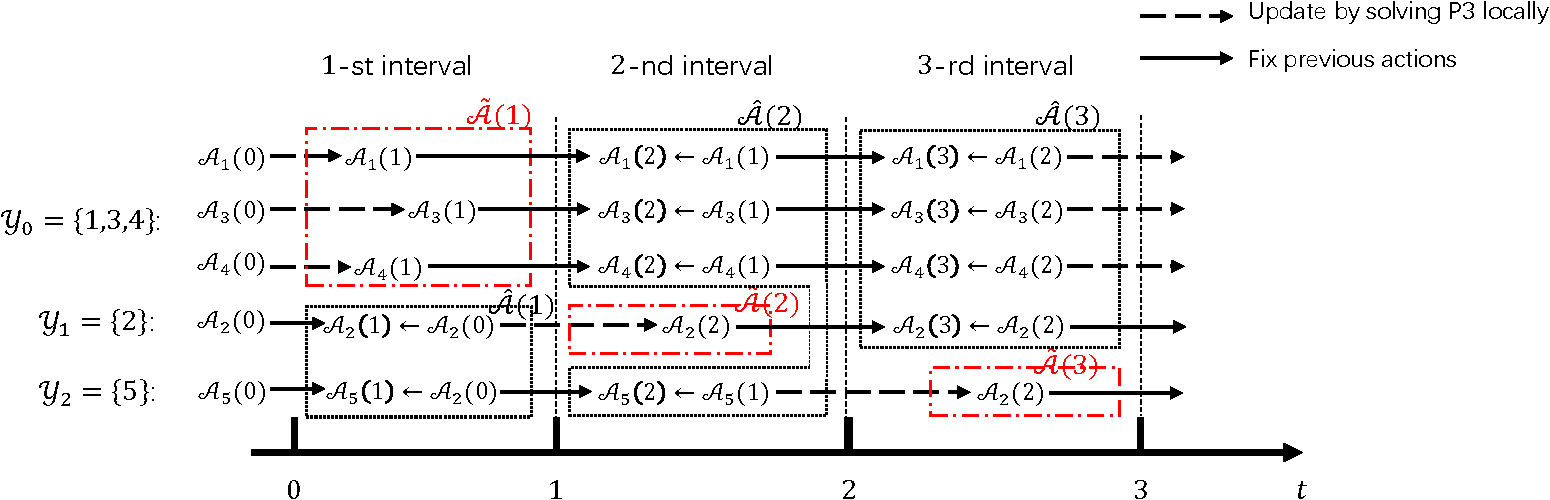
\includegraphics[width=1.0\textwidth]{chapter3/update-timeline.pdf}
        \caption{The Illustration of Example \ref{exp:update}.}
        \label{fig:update_timeline}
    \end{figure*}
\end{example}

As a remark notice that since in Algorithm \ref{alg_1}, the computation complexity at each AP scales linearly with respect to {the size of candidate edge server set}, it can be deployed in a scenario with massive APs and edge servers, as long as the {the number of candidate edge servers for each AP} is limited.

\subsection{Analytical and Semi-Analytical Performance Bounds}
\label{subsec:chapter3-analysis}
In most of the existing approximate MDP solutions \cite{mdp-bound1,mdp-bound2,mdp-bound3}, the performance is difficult to bound analytically as the approximate value function has no accurate meaning on the system cost or utility.
In the proposed algorithm, however, we derive the analytical expression for the baseline policy as the approximate value function.
The following lemma shows this analytical expression is a performance lower bound (cost upper bound) of our proposed policy (Algorithm \ref{alg_1}), {denoted as $\tilde{\Policy}(\Stat(t), \Delay(t))$}.
\begin{lemma}[Analytical Cost Upper Bound]
    \label{lemma:bound}
    Let $W_{\tilde{\Policy}}(\cdot)$ be the value function of the proposed policy $\tilde{\Omega}$, i.e.,
    \begin{align}
        W_{\tilde{\Policy}}(\Stat) \define
        \sum_{t=1}^{\infty} \gamma^{t-1} \mathbb{E}^{\tilde{\Policy}}_{\Delay} \Bracket{
            g\Paren{\Stat(t)} \Big| \Stat(1)=\Stat
        },
        \label{eqn:bound}
    \end{align}
    we have
    \begin{align}
        V(\Stat)
        \leq W_{\tilde{\Policy}}(\Stat)
        \leq W_{\Baseline}(\Stat),
        \forall \Stat.
    \end{align}
    We denote the \emph{$1$-step improved policy} as $\hat{\Baseline}$, which is an intermediate between the baseline policy and the proposed policy. Specifically, $\hat{\Baseline}$ would update the dispatching actions following the Algorithm \ref{alg_1} in the first interval (saying the $t$-th interval) (i.e., at the same time slot with same subset of APs), and then fixes the actions in the following intervals. The explicit definitions are given as follows.
    \begin{align}
        \hat{\Baseline}\Paren{\Stat(t), \Delay(t)} \define 
        \begin{cases}
            \tilde{\Policy}({\Stat(0), \Delay(0)}), &t=1
            \\
            \tilde{\Policy}({\Stat(1), \Delay(1)}), &\text{otherwise}
        \end{cases}.
    \end{align}
    Let $V_{\hat{\Baseline}}(\cdot)$ be the value function of the \emph{$1$-step improved policy} $\hat{\Baseline}$, i.e.,
    \begin{align}
        V_{\hat{\Baseline}}(\Stat) = \mathbb{E}_{\Delay}\Bracket{ g\Paren{\Stat(1)} + \gamma W_{\hat{\Baseline}}\Paren{\Stat(2)} | \Stat(1)=\Stat }.
    \end{align}
    Moreover, as the broadcast interval is random, it is hard to obtain closed-form analytical expression for the tight performance bound $V_{\hat{\Baseline}}(\Stat)$ and a semi-analytical method is proposed.
\end{lemma}
\begin{proof}
    Since the proposed policy $\tilde{\Policy}$ is not optimal policy and $W_{\tilde{\Policy}}(\Stat)$ represents the average system cost with the proposed policy $\tilde{\Policy}$, $V(\Stat) \leq W_{\tilde{\Policy}}(\Stat)$ is straightforward.
    Let 
    \begin{align*}
        \Delta(t) \triangleq &
        \sum_{t'=1}^{\infty} \gamma^{t'-1}
        \mathbb{E}^{ \tilde{\Policy} } \Bracket{
            g\Paren{\Stat(t'), \tilde{\Policy}(\Stat(t'),t-1)}
            -  g\Paren{\Stat(t'), \tilde{\Policy}(\Stat(t'),t)}
        }
    \end{align*}
    denote the improvement of the $t$-th policy update.
    According to Proposition 2.3.3 (a) in \cite{dp-control}, we have $\Delta(t)\geq 0$, $\forall t$.

    Hence, we have
    \begin{align*}
    W_{\Baseline}(\Stat)- W_{\tilde{\Policy}}(\Stat)
    &= 
    \underbrace{\sum_{t'=1}^{N} \gamma^{t'-1} \mathbb{E}^{ \tilde{\Policy} } \Bracket{
        g\Paren{\Stat(t'), \tilde{\Policy}(\Stat(t'),0)}
        - 	g\Paren{\Stat(t'), \tilde{\Policy}(\Stat(t'),t')}
    }}_{\mathfrak{F}(N)}\\
    &+\sum_{t'=N+1}^{+\infty} \gamma^{t'-1} \mathbb{E}^{ \tilde{\Policy} } \Bracket{
        g\Paren{\Stat(t'), \tilde{\Policy}(\Stat(t'),0)}
        - 	g\Paren{\Stat(t'), \tilde{\Policy}(\Stat(t'),t')}
    }\\
    &\geq \mathfrak{F}(N) + \underbrace{\sum_{t'=N+1}^{+\infty} \gamma^{t'-1} \mathbb{E}^{ \tilde{\Policy} } \Bracket{
        g\Paren{\Stat(t'), \tilde{\Policy}(\Stat(t'),0)}
        - 	g_{\max}
    }}_{\mathfrak{G}(N)},
    \end{align*}
    where $g_{\max}$ denotes the upper-bound of the per-stage cost $g(\cdot)$.
    Because  $\mathfrak{F}(N)=\sum_{t=1}^{N}\gamma^{t-1}\Delta(t)\geq 0$, $\mathfrak{F}(N)$ increases as $N$ increases.
    It is obvious that $\mathfrak{G}(N)$ increases as $N$ increases, and 
    \begin{align*}
    \lim\limits_{N\to+\infty}\mathfrak{G}(N)=0
    \end{align*}
    Hence, 
    \begin{align*}
    \exists N,\ \mbox{s.t. }\ W_{\Baseline}(\Stat)- W_{\tilde{\Policy}}(\Stat)\geq \mathfrak{F}(N)-\mathfrak{G}(N) \geq 0.
    \end{align*}
\end{proof}

The above cost upper bound $W_{\Baseline}(\Stat)$ is obtained by assuming all the APs fix the target edge servers for task computation.
Its gap to the performance of the proposed policy, denoted as $W_{\Baseline}(\Stat) - W_{\tilde{\Policy}}(\Stat)$, is mainly due to the adaptive job dispatching of the proposed policy.
Therefore, a tighter semi-analytical cost upper bound is provided below which could be used for quick performance evaluation.
\begin{lemma}[Semi-Analytical Cost Upper Bound]
    Let $\hat{\Baseline}^{(T)}$ denote an intermediate policy, which follows $\tilde{\Policy}$ in the first $T$ intervals and then fixes the policy at the $T$-th interval in the following intervals ($T$ is an arbitrary positive integer), then
    \begin{align}
        W_{\tilde{\Policy}}(\Stat) \leq W_{\hat{\Baseline}}^{(T)}(\Stat)
        \define &\sum_{t=1}^{T} \gamma^{t-1} \mathbb{E}^{\tilde{\Policy}}_{\Delay}\Bracket{g\Paren{\Stat(t)} | \Stat(1)=\Stat}
        \nonumber\\
        &+\gamma^{T} \mathbb{E}^{\Baseline}_{\Stat(T+1)}\Bracket{W_{\Baseline}\Paren{\Stat(T+1)}}.
        \label{eqn:semi-bound}
    \end{align}
    Moreover, the gap $e(T) = W^{(T)}_{\hat{\Baseline}}(\Stat) - W_{\tilde{\Policy}}(\Stat)$ is monotonically decreasing with respect to $T$.
\end{lemma}
\begin{proof}
    Firstly, it is obvious that $W^{(T)}_{\hat{\Baseline}}(\Stat)$ is the cost upper bound for the proposed policy $\tilde{\Policy}$.
    As the Equation (\ref{eqn:bound}) could be split into two parts as shown below,
    \begin{align*}
        W_{\tilde{\Policy}}(\Stat) =
        \sum_{t=1}^{T} &\gamma^{t-1} \mathbb{E}^{\tilde{\Policy}}_{\Delay} \Bracket{ g\Paren{\Stat(t)} | \Stat(1)=\Stat }
        +
        \nonumber\\
        &\gamma^{T} \sum_{t=1}^{\infty} \gamma^{t-1} \mathbb{E}^{\tilde{\Policy}}_{\Delay,\Stat(T+1)} \Bracket{ g\Paren{\Stat(t+T)} },
    \end{align*}
    where the first part is exactly same as the first part in Equation \eqref{eqn:semi-bound} of $W^{(T)}_{\hat{\Baseline}}(\Stat)$, and the second part $\sum_{t=1}^{\infty}\gamma^{t-1}\mathbb{E}^{\tilde{\Policy}}_{\Delay}[g(\Stat(t+T))]$ is upper bounded by $W_{\Baseline}(\Stat(T+1))$ as illustrated in the proof given in lemma \ref{lemma:bound}.

    Then, we show that the performance gap $e(T)$ monotonically decreases with respect to $T$.
    For any positive integer $T$, let
    \begin{align*}
        \Delta{W}(T) \define W^{(T+1)}_{\hat{\Baseline}}(\Stat) - W^{(T)}_{\hat{\Baseline}}(\Stat)
    \end{align*}
    denotes the performance gap due to one-step policy improvement described in Equation (\ref{eqn:partial}).
    According to the \emph{Proposition 2.3.4 (Cost Improvement by Rollout)} in \cite{dp-control}, we have $W^{(T+1)}_{\hat{\Baseline}}(\Stat) \leq W^{(T)}_{\hat{\Baseline}}(\Stat)$ for all $\Stat$.
    Hence, we have $\Delta{W}(T) \geq 0$ for all $T$ and the performance gap $e(T)$ decreases monotonically with respect to $T$.
\end{proof}
In the above cost upper bound, the first item $\sum_{t=1}^{T} \gamma^{t-1} \mathbb{E}^{\tilde{\Policy}}_{\Delay}[g(\Stat(t))]$ has to be evaluated numerically, but the second item $\mathbb{E}^{\Baseline}_{\Stat(T+1)}[{W_{\Baseline}(\Stat(T+1))}]$ can be calculated analytically according to Lemma \ref{lemma:bound}.
The performance of both cost upper bounds will be illustrated in the following simulation section.

%=================================================================================================%
%=================================================================================================%

\section{Reinforcement Learning Algorithm}
\label{sec:chapter3-rl-alg}
Although the approximate value function $W_{\Baseline}(\Stat)$ is derived analytically in the previous section, the calculation of $ W_{\Baseline}(\Stat)$ requires the priori knowledge on the distributions in this system, i.e., the distributions of job arrival, uploading latency and computation time, are usually unknown in advance.
Therefore, we extend the {\Dalgname} with an efficient reinforcement learning approach.
Specifically, with the explicit analytical expressions of $\tilde{W}^{\AP}_{k,m,j}$ and $\tilde{W}^{\ES}_{m,j}$ in Lemma \ref{lemma:w_ap} and Lemma \ref{lemma:w_es}, respectively, we only need to learn the following statistical parameters ($\forall k\in\apSet,m\in\esSet, j\in\jSpace$).
\begin{itemize}
    \item The average arrival rate $\lambda_{k,j}$ of job arrival distribution $B_{k,j}(t)$ , which could be estimated directly from the job arrival events.
    \item The expectation of computation time $c_{m,j}$, which could be estimated on each edge server respectively.
    \item The uploading time distribution $\mathbb{U}_{k,m,j}(\Xi)$ , which could be estimated via the timestamp of each job transmission.
\end{itemize}
Denote the event of type-$j$ job departure from the $m$-th edge server at the $t$-th slot as $\alpha_{m,j}$ (i.e., $\alpha_{m,j}=1$ if there is job departure and $0$ otherwise), the computation time of the departure job as $p^{c}_{m,j}(t)$ and $\vec{u}_{k,m,j} \define [\Pr\{U_{k,m,j}=1\}, \dots, \Pr\{U_{k,m,j}=\Xi\}]$, the reinforcement learning algorithm to track the above statistical parameters is elaborated in Algorithm \ref{alg_2}.
As a remark notice that, the statistical parameters estimation is at time-slot level and could be shared with other APs and edge servers via broadcast information.

\begin{algorithm}[ht]
    \caption{Reinforcement Learning Algorithm}\label{alg_2}
    \DontPrintSemicolon
    \KwIn{$\vec{R}^{(k)}_{m,j}(t)$, $B_{k,j}(t)$, ${p}^{c}_{m,j}(t)$}
    \KwOut{$\hat{\lambda}_{k,j}(t)$, $\hat{c}_{m,j}(t)$, $\hat{\vec{u}}_{k,m,j}(t)$}
    Initialize $\hat{\lambda}_{k,j}(t)$, $\hat{c}_{m,j}(t)$, $\hat{\vec{u}}_{k,m,j}(t)$ as zero ($\forall k\in\apSet,m\in\esSet,j\in\jSpace$).\;
    $t \gets 0, t_c \gets 0$\;
    \While{not converge}{
        $t \gets t + 1$\;
        \ForPar{$k\in\apSet$, $m\in\esSet$, $j\in\jSpace$}{
            $\hat{\lambda}_{k,j}(t) \gets \frac{t-1}{t} \hat{\lambda}_{k,j}(t-1) + \frac{1}{t} I[B_{k,j}(t)=1]$\;
            $\hat{\vec{u}}_{k,m,j}(t) \gets \frac{t-1}{t} \hat{\vec{u}}_{k,m,j}(t-1) + \frac{
                I[\vec{R}^{(k)}_{m,j}(t)=0] \cdot I[\vec{R}^{(k)}_{m,j}(t-1)\neq 0]
            }{
                t || I[\vec{R}^{(k)}_{m,j}(t)=0] \cdot I[\vec{R}^{(k)}_{m,j}(t-1)\neq 0] ||_{2}
            }$\;
            \If{$\alpha_{m,j}==1$}{
                $\hat{c}_{m,j}(t) \gets \frac{t_c-1}{t_c} \hat{c}_{m,j}(t-1) + \frac{1}{t_c} {p}^{c}_{m,j}(t)$\;
                $t_c \gets t_c + 1$\;
            }
        }
    }
\end{algorithm}

It is obvious that when $t\to\infty$, Algorithm \ref{alg_2} will converge, i.e., $\lim_{t\to\infty} \hat{\lambda}_{k,j}(t) = {\lambda}_{k,j}$, $\lim_{t\to\infty} \hat{c}_{m,j}(t) = {c}_{m,j}$ and $\lim_{t\to\infty} \hat{\vec{u}}_{m,j}(t) = \vec{u}_{m,j}$ ($\forall k\in\apSet,m\in\esSet,j\in\jSpace$).

\begin{remark}[Learning Efficiency of Algorithm \ref{alg_2}]
    In conventional reinforcement learning algorithms, the value function should be evaluated for at least a large subset of system states or state-action pairs (e.g., Q-learning) before the convergence.
    Moreover, the value function of a system state can be updated only when this system state appears after state transitions (which is impractical for our problem which is with enormous state space or action space), which leads to large computation complexity and convergence time.
    In the proposed reinforcement learning algorithm, however, we only learn the unknown statistics of the value function by tracking their unbiased observations.
    Hence, the proposed algorithm could converge faster.
\end{remark}

%=================================================================================================%
%=================================================================================================%

\section{Performance Evaluation}
\label{sec:chapter3-evaluation}
In this section, we evaluate the performance of the proposed low-complexity dispatching policy $\tilde{\Policy}$ by numerical simulations.
The experiment setup and performance benchmarks are elaborated in Section \ref{subsec:chapter3-setup}.
The simulation results are illustrated in Section \ref{subsec:chapter3-basic}.
The sensitivity study on parameters is also applied to provide some insights on the robustness of the proposed policy in Section \ref{subsec:chapter3-advance}.

\subsection{Experiment Setup}
\label{subsec:chapter3-setup}
In the simulation, we assume that there are $K=15$ APs, $M=10$ edge servers and $J=10$ types of jobs in the system.
One broadcast interval consists of $t_{B}=25$ time slots.
The network topology is generated according to Barab\'asi-Albert (BA) model \cite{albert1999diameter}.
The edge servers are randomly placed collocated with the APs.
Under this network topology setup with degree as $3$, the subset partition algorithm \ref{alg_0} could reduce the update period $N$ from $15$ to $6$ time slots.

The BA model is parameterized by $n$ and $m$ and produces a graph with $n$ vertices and $m$ edges such that the degree distribution follows a power-law.
The arrival traces and job processing time for each job type are extracted from Google cluster traces \cite{clusterdata:Reiss2011} and then randomly assigned on APs and edge servers, respectively.
The maximum uploading latency is $\Xi = 3t_B$, and the distribution of $\mathbb{U}_{k,m,j}(\Xi)$ ($\forall k\in\apSet, m\in\esSet_{k}, j\in\jSpace$) is arbitrarily generated within the support $\set{0, 1, \dots, \Xi}$.
The {\brlatency} is with an integer support from $0.7t_B$ to $0.9t_B$ time slots.
Each queue for VM on edge server is with maximum queue length $L_{max}=50$, i.e., there would be at most $50$ jobs on one edge server.
The discount factor $\gamma$ is $0.95$ and the overflow penalty weight $\beta$ is $120$.

%-----------------------------------------------------------------------%
\begin{figure*}[ht]                                                      %
    \centering                                                          %
    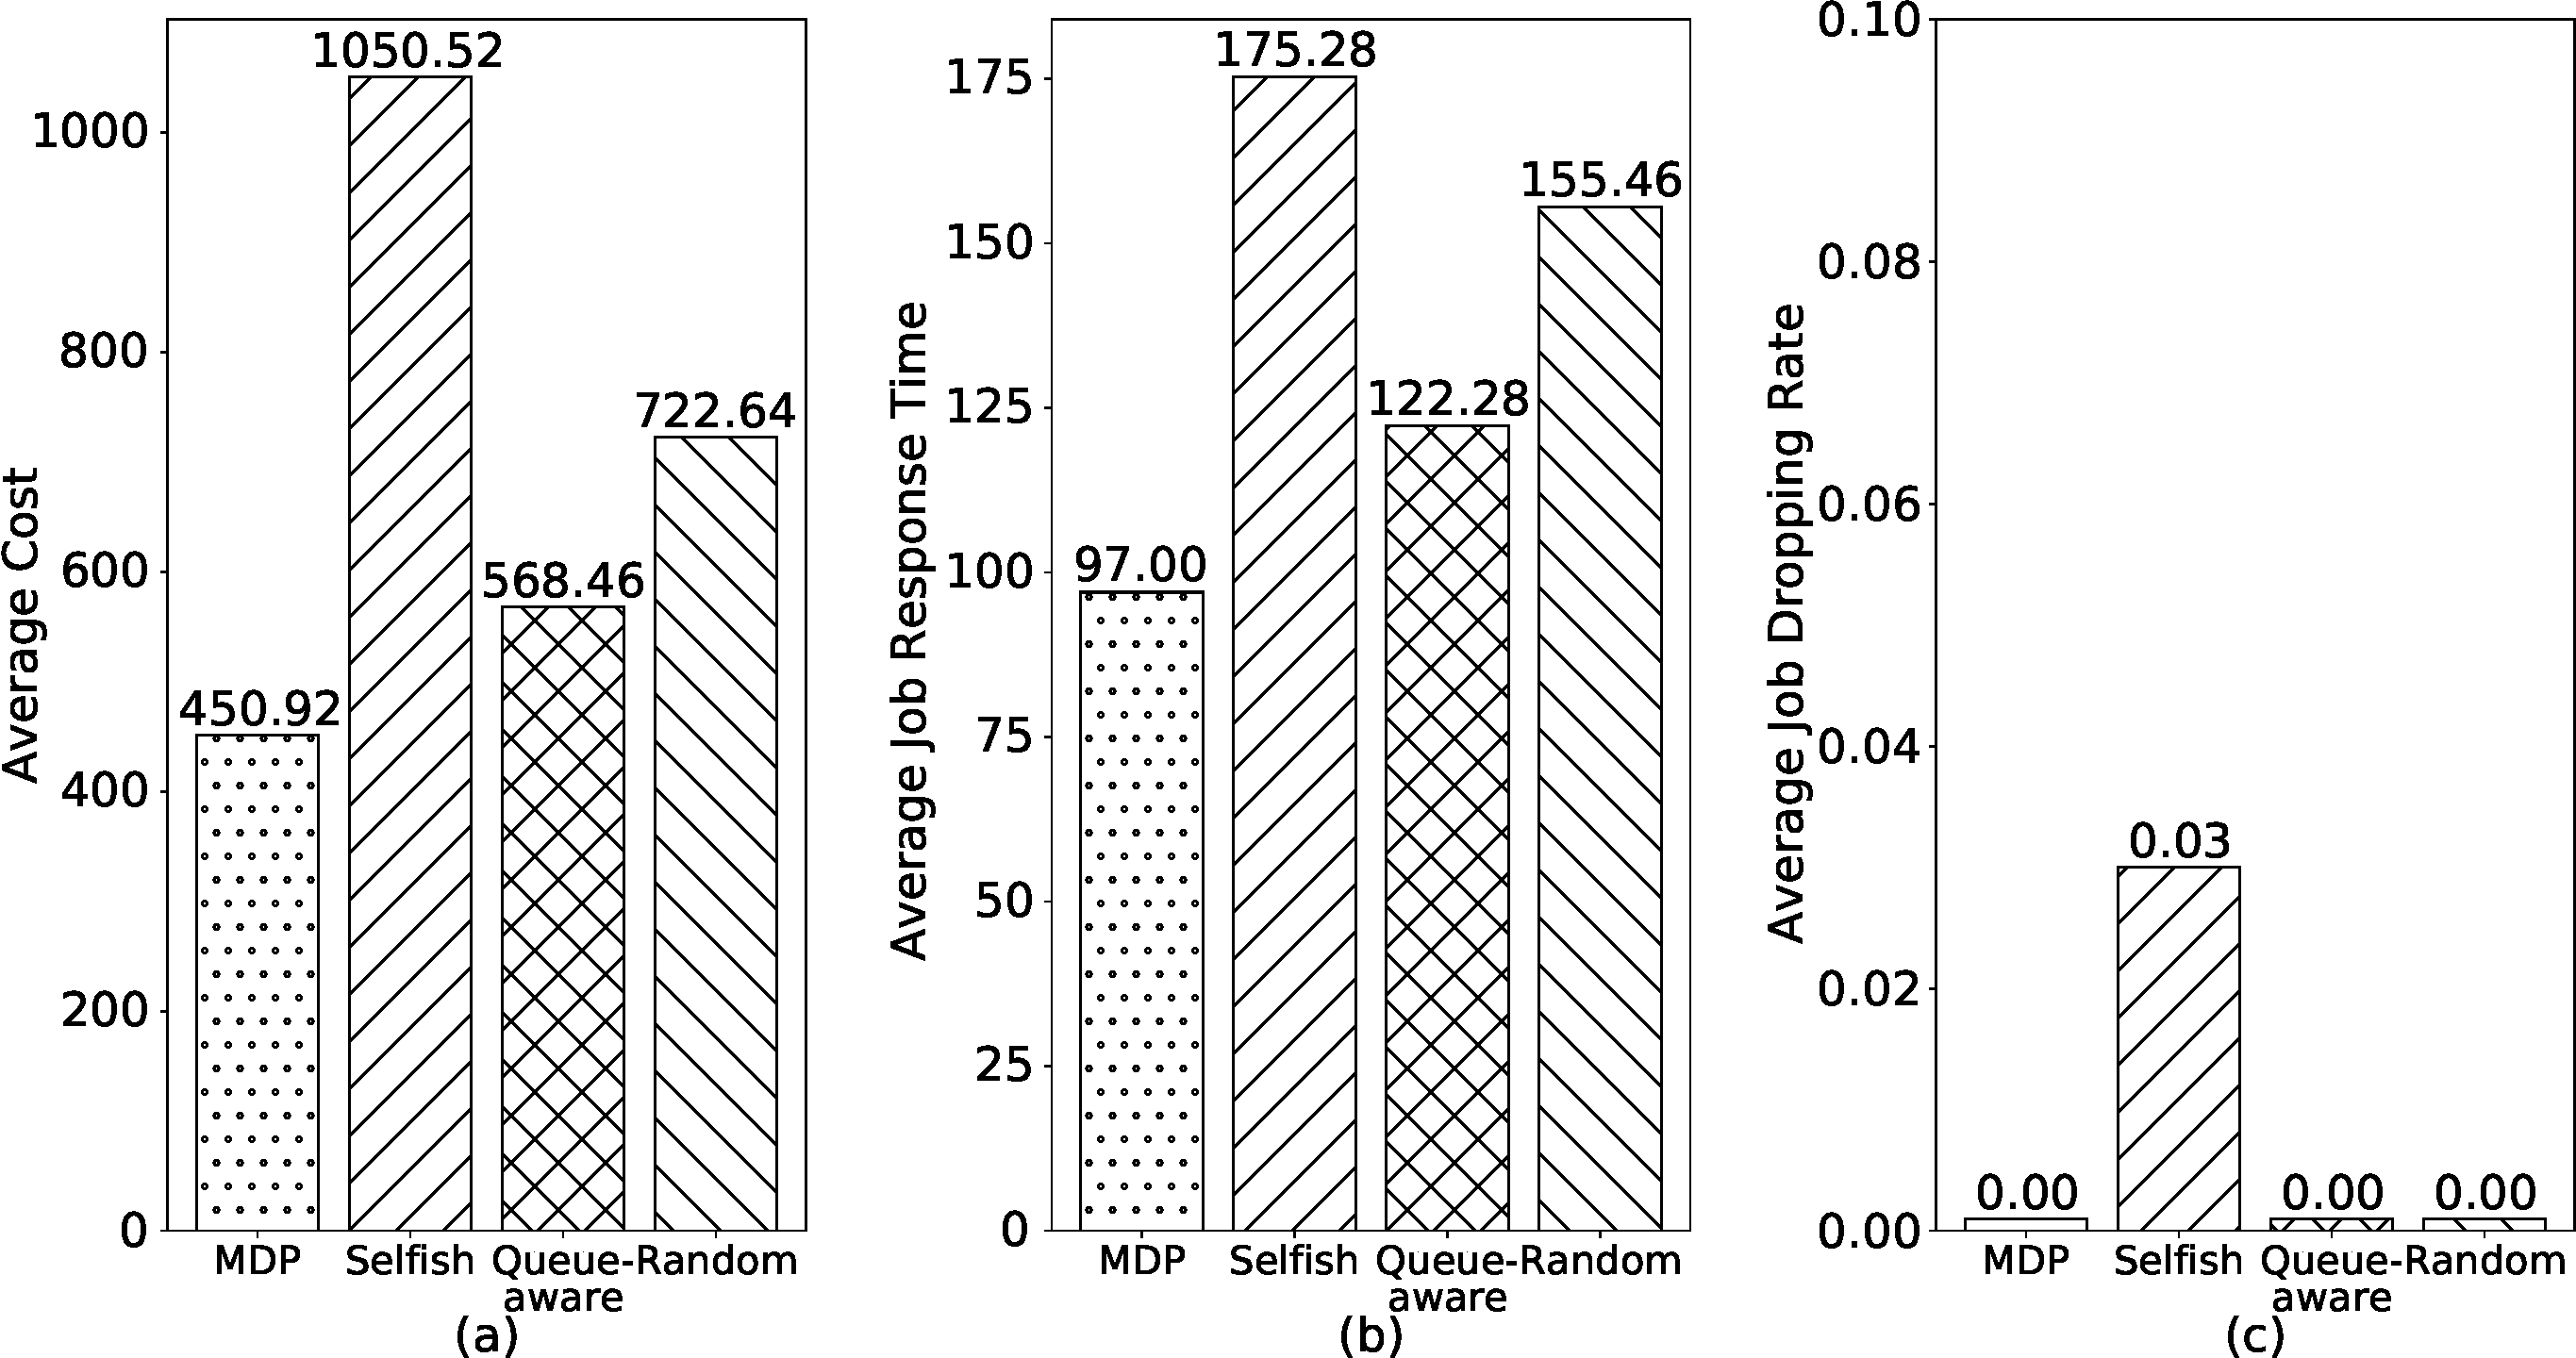
\includegraphics[width=1.0\textwidth]{chapter3/the-bar-graph-alt.pdf}               %
    \caption{Illustration of performance metrics comparison with benchmarks.}
    \label{fig:bar_plot}                                                %
\end{figure*}                                                            %
%-----------------------------------------------------------------------%

%NOTE: Benchmark Elaboration
We also propose three heuristic benchmarks to profile the performance of the proposed solution framework {\Dalgname}, which are listed as follows.
\begin{itemize}
    \item \textbf{Random Policy}:
            Randomly choose a dispatching edge server in each time slot; 
    \item \textbf{Selfish Policy}:
            Always choose the edge server with the minimum sum of the expected uploading time and processing time;
    \item \textbf{Queue-aware Policy}:
            Always choose the edge server with the minimum sum of expected uploading time, processing time and queueing time based on the observation of outdated queue status.
\end{itemize}
Moreover, we choose the Selfish Policy as the initial dispatching action (Baseline Policy) for our proposed algorithm (Algorithm \ref{alg_1}).

%NOTE: Basic Performance
\subsection{Performance Analysis}
\label{subsec:chapter3-basic}
As illustrated in \figurename~\ref{fig:bar_plot}(a), the proposed policy (MDP Policy) outperforms all the benchmarks in the average system cost.
Moreover, the Queue-aware Policy has better performance than the other benchmarks due to its capability of adapting dispatching action according to the outdated observation of queueing state.
More insights on the performance comparison are provided in \figurename~\ref{fig:bar_plot}(b) and (c).

In the former figure, the average job response times, measuring the average number of broadcast intervals from job's arrival at one AP to the completeness of computation at one edge server, are compared.
It can be observed that the proposed policy still outperforms all the benchmarks.
In \figurename~\ref{fig:bar_plot}(c), the job dropping rates, measuring the ratio of jobs dropped by edge servers due to queue overflow, are also compared.
{In} summary, the proposed policy outperforms {the} other three benchmarks with the minimum average cost and job response time.
{Moreover, there {are} no dropping jobs incurred compared with the Selfish policy, which is the initial baseline policy for our proposed algorithm.}

Finally, a realization of job dispatching is illustrated in \figurename~\ref{fig:general_timeline}, where the number of jobs in the system is plot versus the index of broadcast interval.
It can be observed that the proposed policy {manages} to keep the number of jobs {at a} lower level, compared with the other benchmarks.
This demonstrates its high dispatching efficiency.

In \figurename~\ref{fig:semi-bound}, the simulation result demonstrates the vanishing gap between the semi-analytical cost upper bound $W^{(T)}_{\hat{\Baseline}}(\Stat)$ and the actual average performance of the proposed policy for different $T$.
It shows that the proposed policy $\tilde{\Policy}$ is bounded and the performance gap $e(T)$ decreases monotonically when $T$ increases, leading to a trade-off between evaluation accuracy and computation complexity.

%-----------------------------------------------------------------------------------------------%
\begin{figure*}[ht!]                                                                             %
    \centering                                                                                  %
    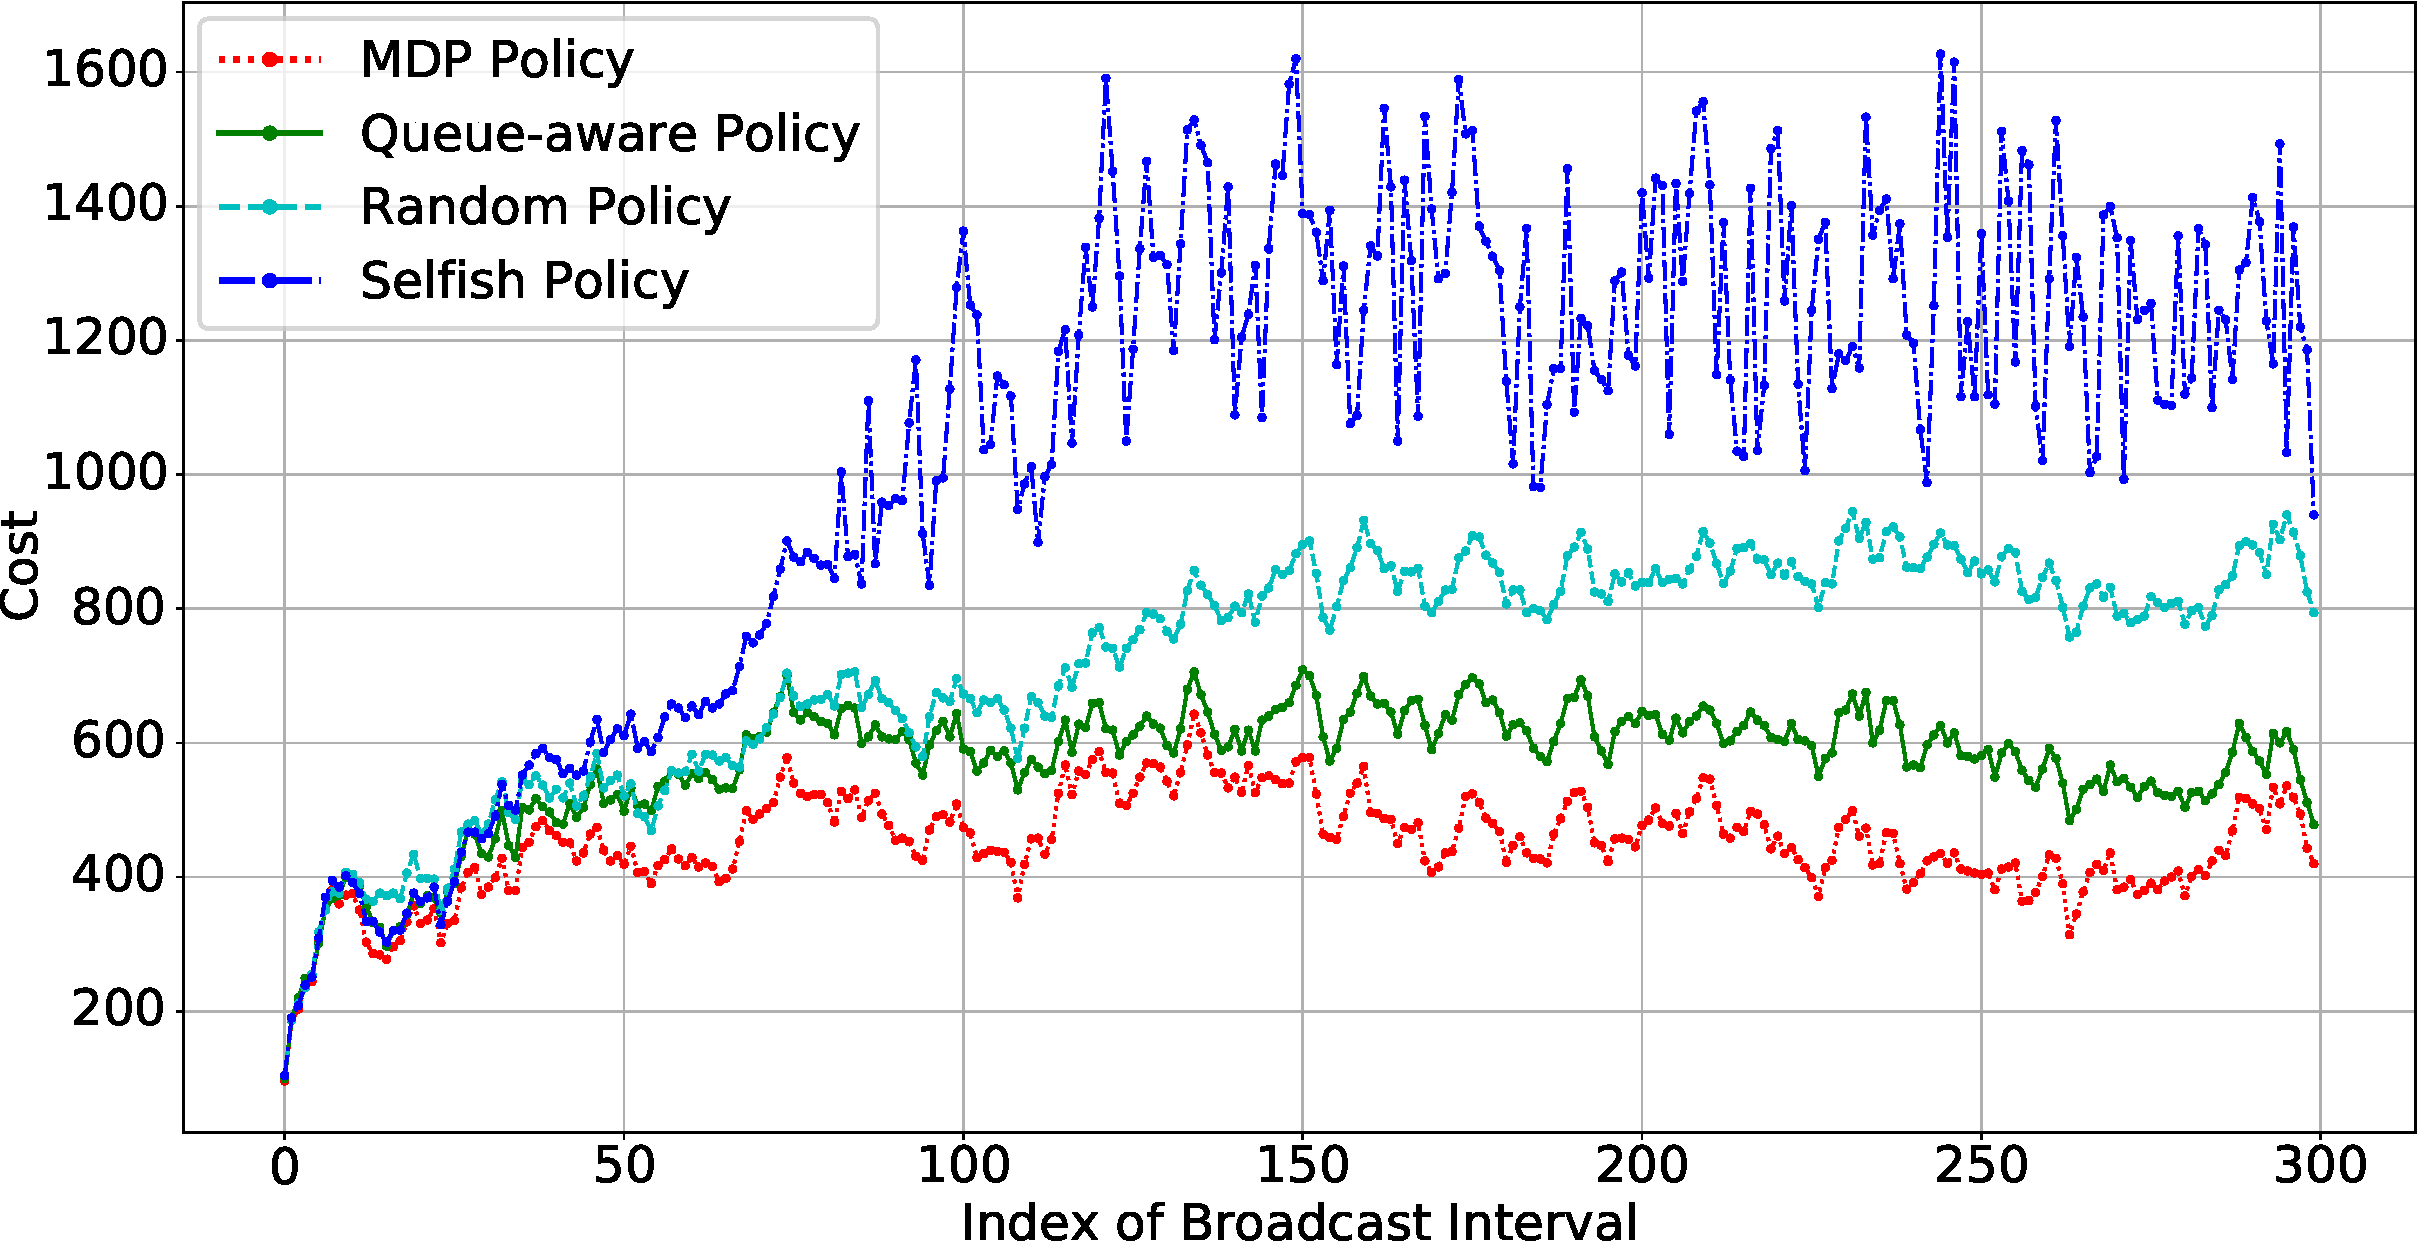
\includegraphics[width=1.0\textwidth]{chapter3/the-cost-timeline-alt.pdf}                     %
    \caption{Illustration of cost versus index of broadcast interval.}
    \label{fig:general_timeline}                                                                %
\end{figure*}                                                                                    %
%-----------------------------------------------------------------------------------------------%

%-----------------------------------------------------------------------------------------------%
\begin{figure*}[ht!]                                                                             %
    \centering                                                                                  %
    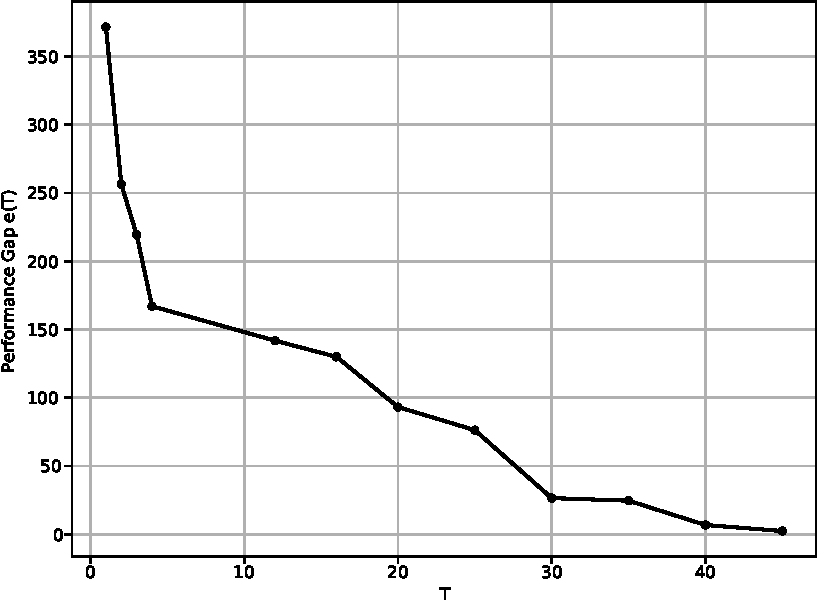
\includegraphics[width=1.0\textwidth]{chapter3/the-semi-bound-analysis.pdf}                     %
    \caption{Illustration of performance gap between $W^{(T)}_{\hat{\Baseline}}(\Stat)$ and $W_{\tilde{\Policy}}(\Stat)$ versus the stage number of numerical evaluation T.}
    \label{fig:semi-bound}                                                                %
\end{figure*}                                                                                    %
%-----------------------------------------------------------------------------------------------%

%NOTE: Reinforcement Learning Analysis
\subsection{Convergence Analysis}
\label{subsec:chapter3-converge}
The convergence property of the proposed reinforcement learning algorithm is illustrated in \figurename~\ref{fig:rl_plot}.
It can be observed that the learning procedures for all the three statistical parameters converge after $80$ broadcast intervals.
On the other hand, the number of observations required for the convergence of conventional reinforcement learning algorithms is usually larger for enormous system and action space.
This demonstrates the efficiency of the proposed reinforcement learning algorithm, which benefits from the derived expression {of} the approximate value function.
\begin{figure*}[ht!]
    \centering
    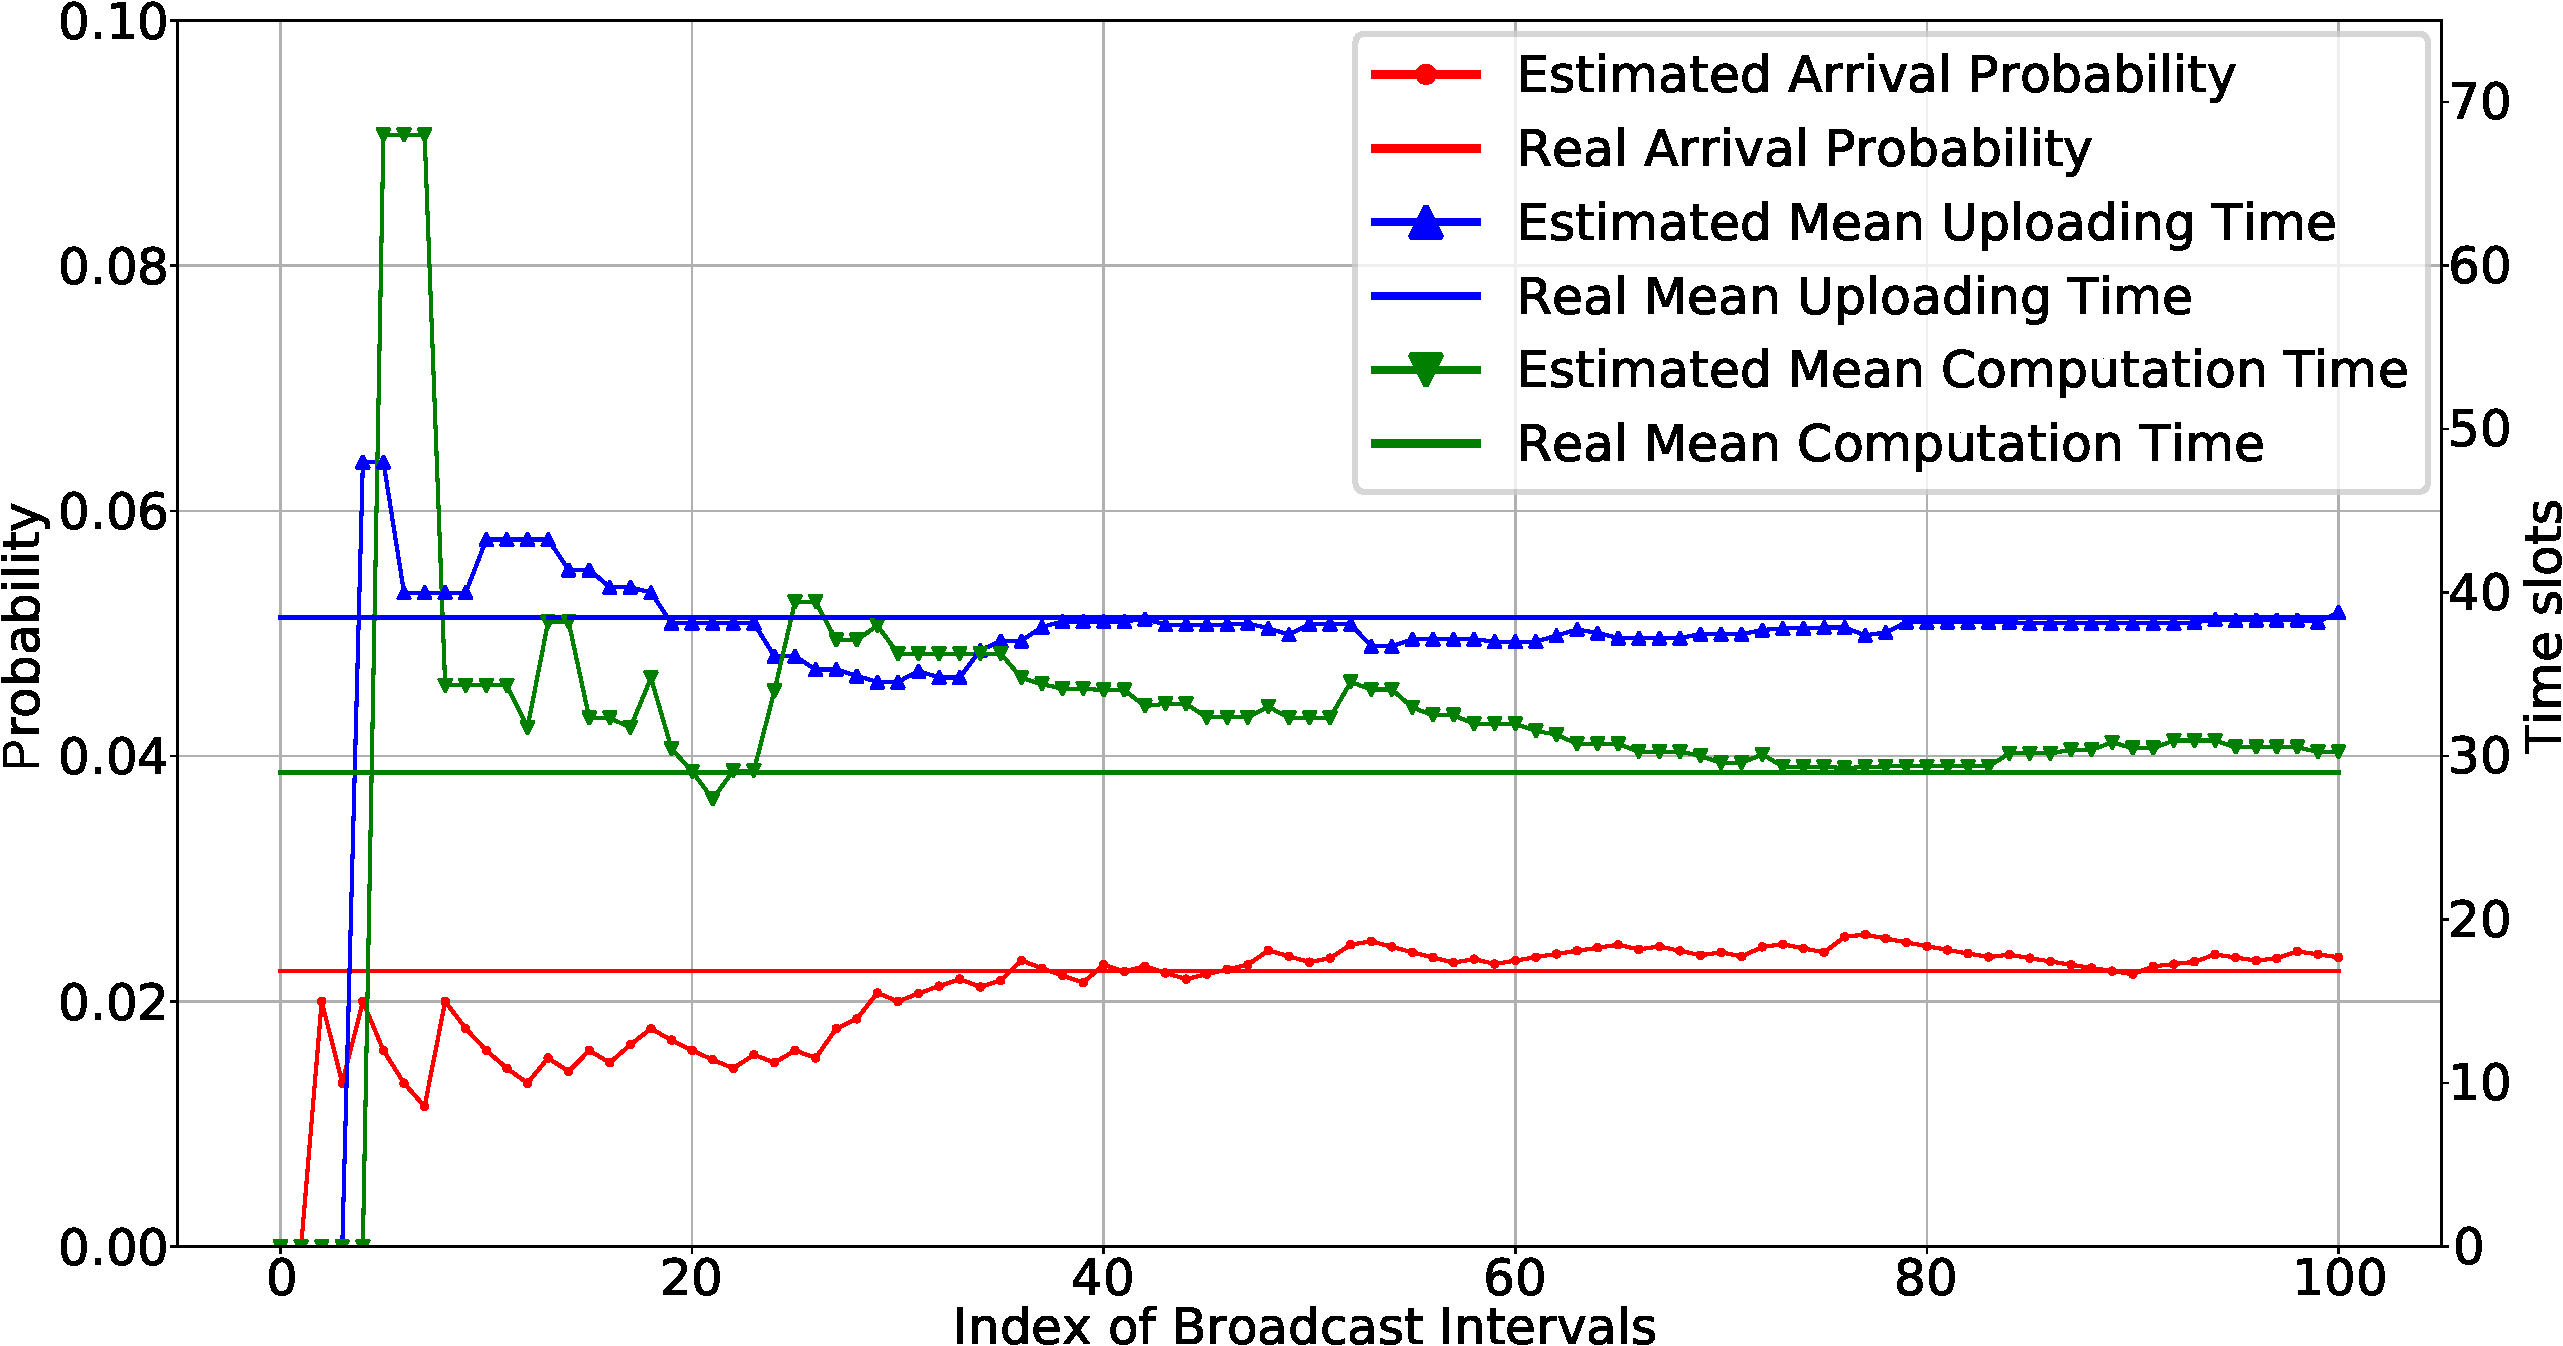
\includegraphics[width=1.0\textwidth]{chapter3/the-rl-fitting.pdf}
    \caption{Illustration of reinforcement learning algorithm.} 
    \label{fig:rl_plot}
\end{figure*}

\subsection{Sensitivity Study}
\label{subsec:chapter3-advance}
%-----------------------------------------------------------------------------------%
\begin{figure*}[ht!]                                                                %
    \centering                                                                      %
    \begin{minipage}[b]{0.65\textwidth}                                             %
        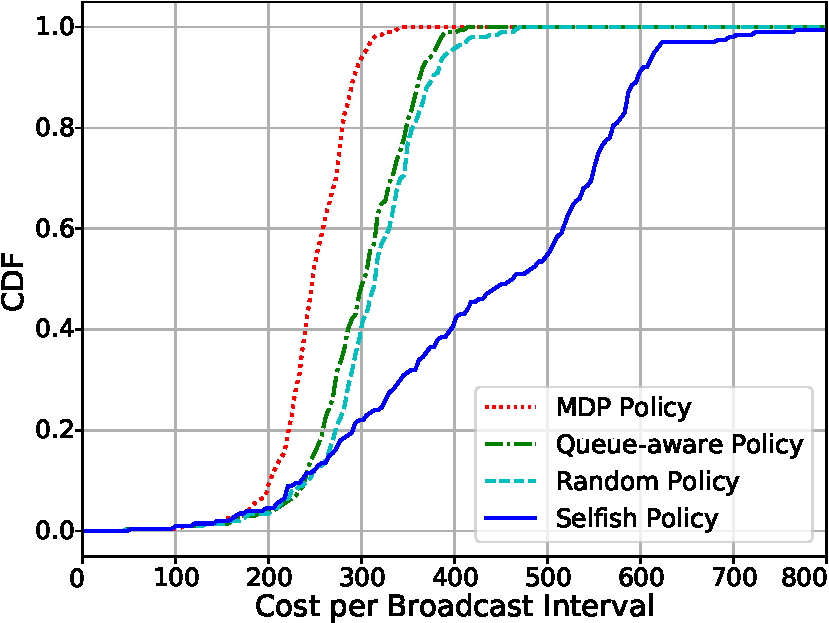
\includegraphics[width=\textwidth]{chapter3/the-delay-small.pdf} \\         %
        (a) Latency = $5$ time slots                                                %
        %\\ % extra filling line                                                    %
    \end{minipage}                                                                  %
    \begin{minipage}[b]{0.65\textwidth}                                             %
        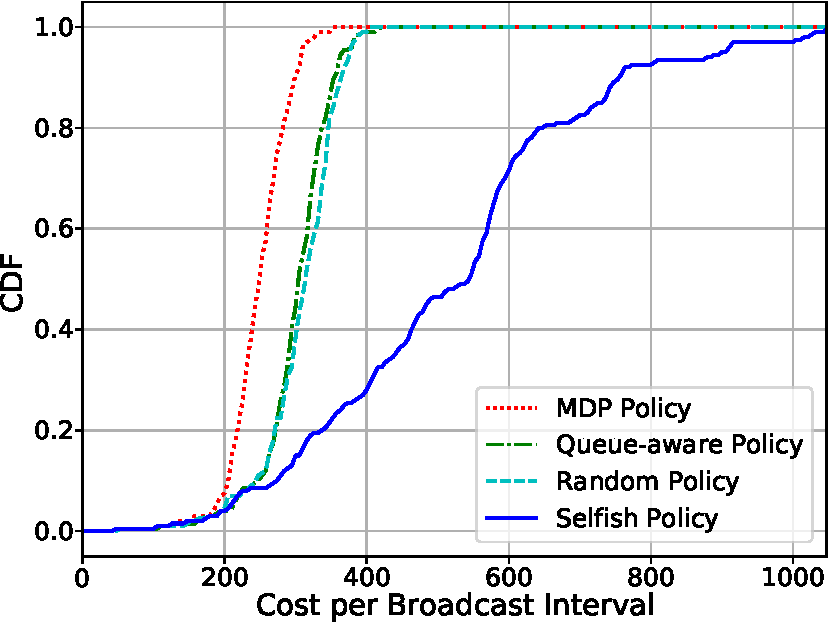
\includegraphics[width=\textwidth]{chapter3/the-delay-medium.pdf} \\        %
        (b) Latency = $12$ time slots                                               %
    \end{minipage}                                                                  %
    \begin{minipage}[b]{0.65\textwidth}                                             %
        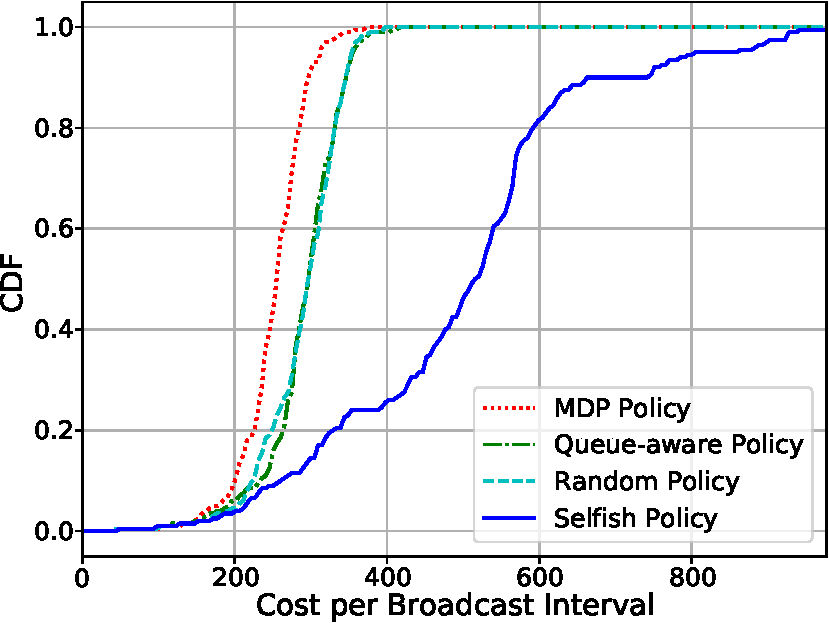
\includegraphics[width=\textwidth]{chapter3/the-delay-large.pdf} \\         %
        (c) Latency = $25$ time slots                                               %
    \end{minipage}                                                                  %
    \caption{Algorithm Robustness versus various signaling latency.}                %
    \label{fig:ss_signal}                                                           %
\end{figure*}                                                                       %
%-----------------------------------------------------------------------------------%


%-------------------------------------------------------------------%
\begin{figure*}[hbt]                                                 %
    \centering                                                      %
    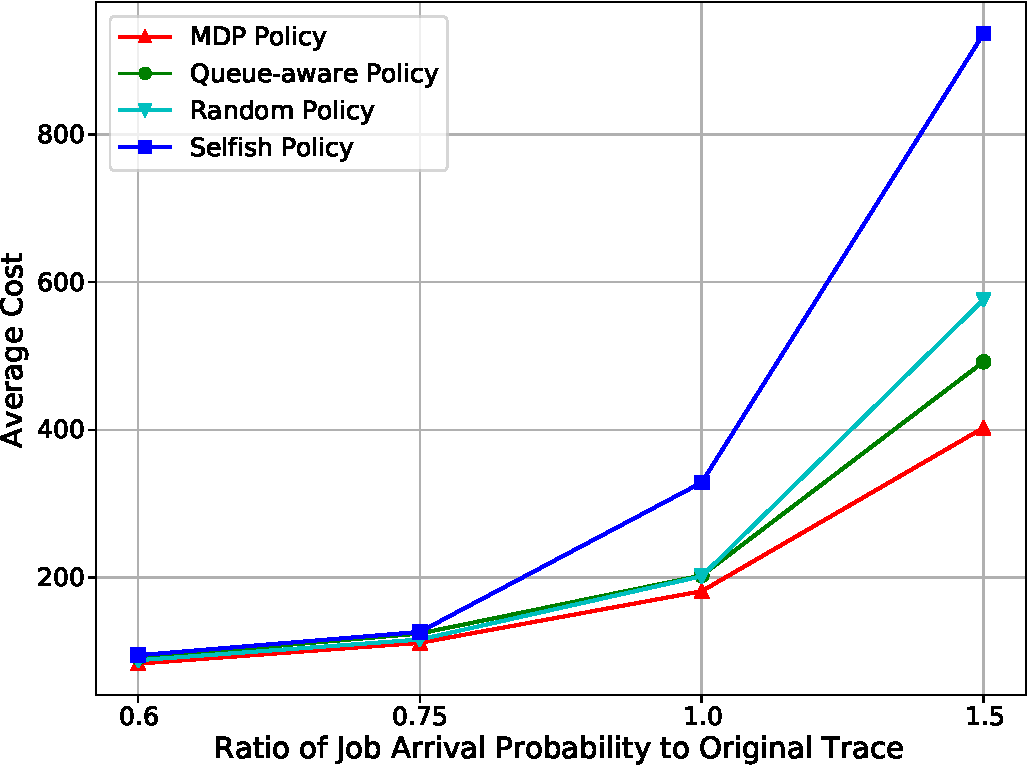
\includegraphics[width=1.0\textwidth]{chapter3/the-arrival-study.pdf}   %
    \caption{Illustration of average system cost versus job arrival intensity.}
    \label{fig:ss_scale}                                            %
\end{figure*}                                                        %
%-------------------------------------------------------------------%

%-------------------------------------------------------------------%
\begin{figure*}[hbt]                                                 %
    \centering                                                      %
    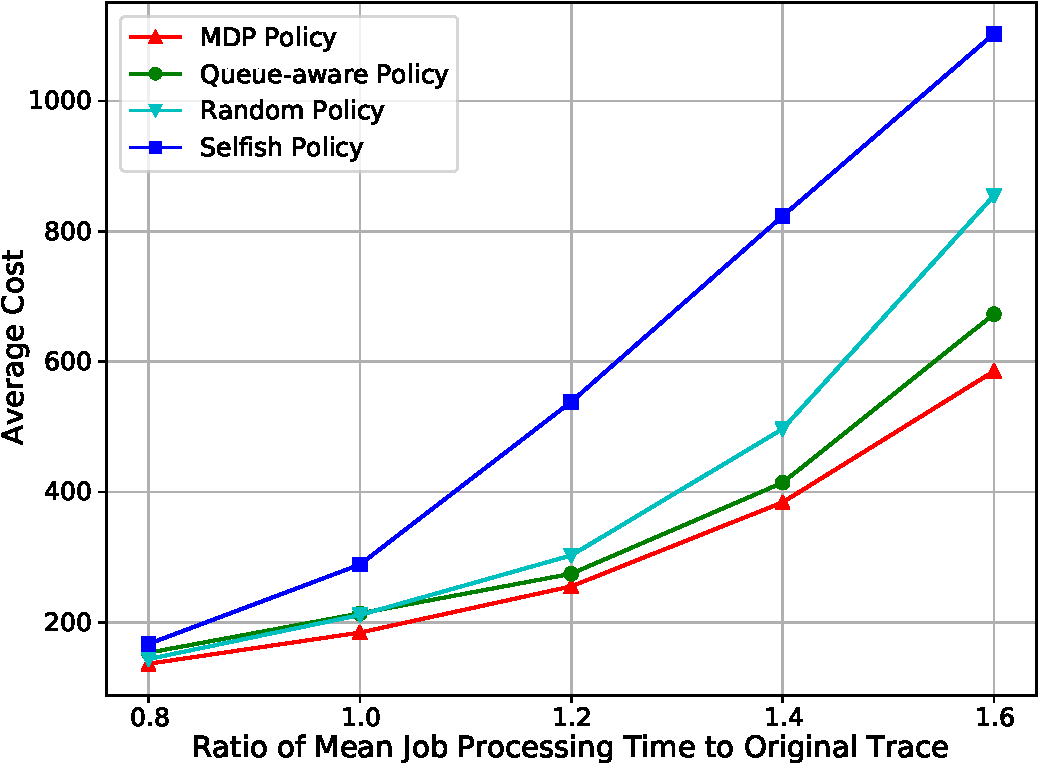
\includegraphics[width=1.0\textwidth]{chapter3/the-proc-study.pdf}      %
    \caption{Illustration of average system cost versus mean processing time.}
    \label{fig:ss_dist}                                             %
\end{figure*}                                                        %
%-------------------------------------------------------------------%

%NOTE: sensitivity study
\noindent\textbf{Signaling Latency.}
The simulation results with different {\brlatency} $\mathcal{D}_{k}$ ($\forall k\in\apSet$) are illustrated in \figurename~\ref{fig:ss_signal}, where the cumulative distribution function (CDF) of the job number in the system is plotted.
Specifically, the {\brlatency} of all the APs is set to $5, 12, 25$ in \figurename~\ref{fig:ss_signal}(a), \figurename~\ref{fig:ss_signal}(b), \figurename~\ref{fig:ss_signal}(c), respectively.
It can be observed from \figurename~\ref{fig:ss_signal}(a) to \figurename~\ref{fig:ss_signal}(c) that, with the increasing of {\brlatency}, the performance of Queue-aware Policy becomes worse.
The Queue-aware policy slightly outperforms the Random Policy in \figurename~\ref{fig:ss_signal}(a) with smaller {\brlatency} (achieving a smaller number of jobs in the system), and becomes worse in \figurename~\ref{fig:ss_signal}(c) with large {\brlatency}.
This demonstrates that the Queue-aware Policy is sensitive to the {\brlatency}.
In all the figures, the proposed policy outperforms all the benchmarks, which demonstrates its robustness versus signaling latency.

\noindent\textbf{Job Arrival Probability.}
We carry out the sensitivity study of job arrival probability by scaling the interval of jobs arriving in Google cluster traces.
The average system cost versus the number of APs is illustrated in \figurename~\ref{fig:ss_scale}.
With the {increase} of job arrival probability, the average system cost increases in all the benchmarks and our proposed policy.
It can be observed that our policy performs the best.
Moreover, the performance gain becomes significant when the computation load is heavy.
This demonstrates the dispatching efficiency of the proposed policy with heavy load.
The gain is negligible for light load, where the computation capability is sufficient and dispatcher optimization may not be necessary.

\noindent\textbf{Mean Processing Time.}
The simulation results with different mean processing time $\set{c_{m,j}|\forall m\in\esSet,j\in\jSpace}$ are illustrated in \figurename~\ref{fig:ss_dist}, where the average processing time from Google cluster traces is scaled by a factor from $0.8$ to $1.6$ respectively.
in our computation model assumption.
Generally speaking, with the increasing average processing time, the average system cost increases in all the benchmarks and our proposed policy.
The simulation results are consistent with that in \figurename~\ref{fig:ss_scale}.
It can be observed that the proposed policy has better performance than the benchmarks.
Moreover, the performance gain becomes significant when the computation time is long.

%=================================================================================================%
%=================================================================================================%

\section{Summary}
\label{sec:chapter3-conclusion}
In this chapter, we consider a distributed and asynchronous job dispatching design in an edge computing network residing in a MAN with multiple APs and edge servers.
The APs and edge servers periodically broadcast their local state information to facilitate distributed dispatcher design.
Due to random transmission latency, the system information observed at different dispatchers are asynchronous.
We also consider a practical scenario that not all the state information can be observed by each AP.
Hence, the distributed optimization of job dispatching strategies at all the APs is formulated as a POMDP, whose minimization objective is a discount measurement of job delivery and computation time.
We propose a novel low-complexity distributed solution framework, called {\Dalgname}, based on analytical approximation of value function and one-step policy iteration, where the complicated POMDP solution or value iteration is avoided. Both the analytical and semi-analytical performance lower bounds are derived for the approximate MDP solution.
Furthermore, to handle a general scenario where the statistics of signaling latency, uploading latency and computation time are unknown in advance, an efficient online learning approach is proposed.
The simulation results show that the proposed solution framework outperforms various heuristic baselines.

        %%% Part II
        \part{Low-complexity Algorithm Design for Multi-agent Edge Learning Systems} %Infinite-horizon Large-scale MDP
        \label{part_2}
        % !TeX root = ../../main.tex

\chapter{FedCars: A Data-Driven Uplink Scheduling Framework for Efficient In-Vehicle Federated Edge Learning}
\label{ch2}

%NOTE: (1) federated learning for autonomous driving
Machine learning, especially deep learning, is becoming one of the enabling techniques of autonomous driving \cite{ad-survey}.
Due to the requirement of timely model training in autonomous driving, edge federated learning is a promising technology to relieve uploading load of the cellular network and computation burden at the edge server, which offloads the model training to the edge devices.
In this Chapter, we consider the scheduling of model uploading in a vehicular edge federated learning system, where the {\IAVs} are deployed with multi-modal sensors and the model training is conducted in a federated learning scenario.
In the model training phase, the {\IAVFullnames} ({\IAVs}) are deployed with a variety of multi-modal sensors, e.g., cameras, LiDRAs and radars, to collect the sensing data for the cooperative training of a deep neural network, e.g., SECOND \cite{SECOND}.
They usually generate a dataset up to terabytes.
Since the raw data collected on {\IAVs} is of high redundancy between adjacent time slots, and the online in-vehicle training of federated learning, e.g., via semi-supervised federated learning framework \cite{icra2021-hong}, could suppress the unnecessary cost of data uploading \cite{vfl-survey}.
However, the model uploading in the federated learning still consumes significant transmission time and energy. In this chapter, we would like to relieve this burden by exploiting the prediction of {\IAVs}' random trajectories in model uploading.

%NOTE: (2) related works for FL on vehicles
% deterministic optimization for data uploading or offloading
Usually, the communication and computation scheduling for vehicle networks couples tightly with the vehicular trajectories, which refer to the vehicles' locations versus time.
There are amount of works considering the scheduling of communication, edge computing or edge learning in vehicle networks with deterministic trajectories
\cite{Globecom18-Wang, Access19-Xu, TITS21-Xiao, JSAC23-Pervej, IOTJ22-Lv, TVT22-Hui},
i.e., the future locations of vehicles could be planned or known in advance.
For example, in \cite{Globecom18-Wang}, the scenario that multiple vehicles move along one unidirectional road at a constant speed and offload the computation tasks to one base station (BS) located along the road was considered. A heuristic scheme was proposed to suppress the delay of task offloading via vehicle-to-vehicle (V2V) communications.
The edge computing scenario with multiple BSs and disjoint coverage was then investigated in \cite{Access19-Xu}. A genetic algorithm was proposed to make the task offloading decision, such that a good trade-off between the total turn-around time and the total resource utility could be achieved.
In \cite{TITS21-Xiao}, the weighted summation of time and energy consumption is minimized in vehicular federated learning, where the velocities of vehicles and the transmission data rate are assumed to be constant. 
Although most of the related works assumed deterministic trajectory, the actual velocities of the vehicles are random, depending on road map, population distribution, working hours, car-holding rate, driving habits and etc. The above scheduling design based on deterministic optimization could not be directly applied, as scheduling with random trajectory might be stochastic optimization problems.

% stochastic optimization for offloading
There have been a few works on the scheduling of data communication or edge computing in vehicle networks with random traffic (random trajectory)
\cite{TVT18-Ni, Access19-Liu, TVT19-Liu, WC16-Salahuddin, TITS16-Wang}.
For example, in \cite{TVT18-Ni}, a hybrid vehicle-to-vehicle (V2V) and vehicle-to-infrastructure (V2I) network was considered with random inter-vehicle distance, where a heuristic strategy was proposed to cluster the vehicles and maximize the expected communication capacity.
In \cite{Access19-Liu}, continuous task offloading from single vehicle to multiple edge servers was optimized via the Q-learning with the average task turn around time as the minimization objective. However, it is difficult to extend the Q-learning method to multi-vehicle scenario, due to the curse of dimensionality.
In \cite{TVT19-Liu}, the scenario that both fixed edge servers and mobile vehicular servers would provide computation service to multiple user equipment was investigated. The Deep Q-Network (DQN) was leveraged to learn the offloading and power allocation decisions, such that the average total communication and computation cost of all UEs was minimized. However, the model training might be of significant computation complexity and the performance can hardly be bounded analytically with the method of DQN. Moreover, the models of random traffic in the above works might be too ideal to fit the real applications. Hence, there are still some open issues on the scheduling algorithm design for vehicle networks:
\begin{enumerate}
    \item How to depict the randomness of vehicular trajectory resembling the real-world statistics, instead of assuming it in trivial form like Gaussian distribution?
    \item How to efficiently and reliably handle long-term and large-scale online resource allocation for vehicle networks with random traffic?
\end{enumerate}

To shed some lights on the above issues, we particularly consider the scenario of in-vehicle federated learning, and  propose a data-driven optimization framework, namely {\fwName}, for scheduling of the model uploading. In fact, the scheduling of model uploading for multiple vehicles with random trajectories is a finite-horizon Markov Decision Process (MDP), where the complexity of optimal solution grows exponentially with respect to the vehicle number. The {\fwName} aims to exploit the statistical knowledge on the trajectories of vehicles and provide a low-complexity scheduling solution with a good performance, where our contributions are summarized below.
\begin{itemize}
    \item We develop the {\fwName} simulator to obtain high-fidelity trajectory dataset of {\IAVs} for customizable traffic scenarios, such that the random trajectories of vehicles can be modelled as Markov chains via statistical learning and predicted in online scheduling. Thus, our algorithm design is based on the high-fidelity traffic statistics.
    \item We propose a two-time-scale algorithm, namely {\fwName} optimizer, to find a sub-optimal policy with low complexity. Moreover, the scheduling according to {\fwName} optimizer is with a non-trivial analytical performance bound. The simulation results show that the {\fwName} optimizer outperforms various baselines under different settings, and achieves good balance between computational complexity and optimality.
\end{itemize}

The remainder of this chapter is organized as follows.
In Section \ref{sec:chapter2-model}, the traffic model of {\IAVs}, as well as the models of uplink queuing and data transmission, is described.
In Section \ref{sec:chapter2-formulation}, the communication scheduling problem is formulated as a finite-horizon MDP, the structure and challenge of optimal solution is discussed.
In Section \ref{sec:chapter2-framework}, the {\fwName} simulator and the statistical learning for the vehicles' random trajectories are elaborated.
Then, the {\fwName} optimizer is introduced in Section \ref{sec:chapter2-new_framework}, \ref{sec:chapter2-kernel-policy} and \ref{sec:chapter2-local-policy}.
Finally, the numerical simulation is presented in Section \ref{sec:chapter2-simulation} and the conclusion is drawn in Section \ref{sec:chapter2-conclusion}.


%=================================================================================================%
%=================================================================================================%

\section{System Model}
\label{sec:chapter2-model}

\begin{figure*}[htp!]
    \centering
    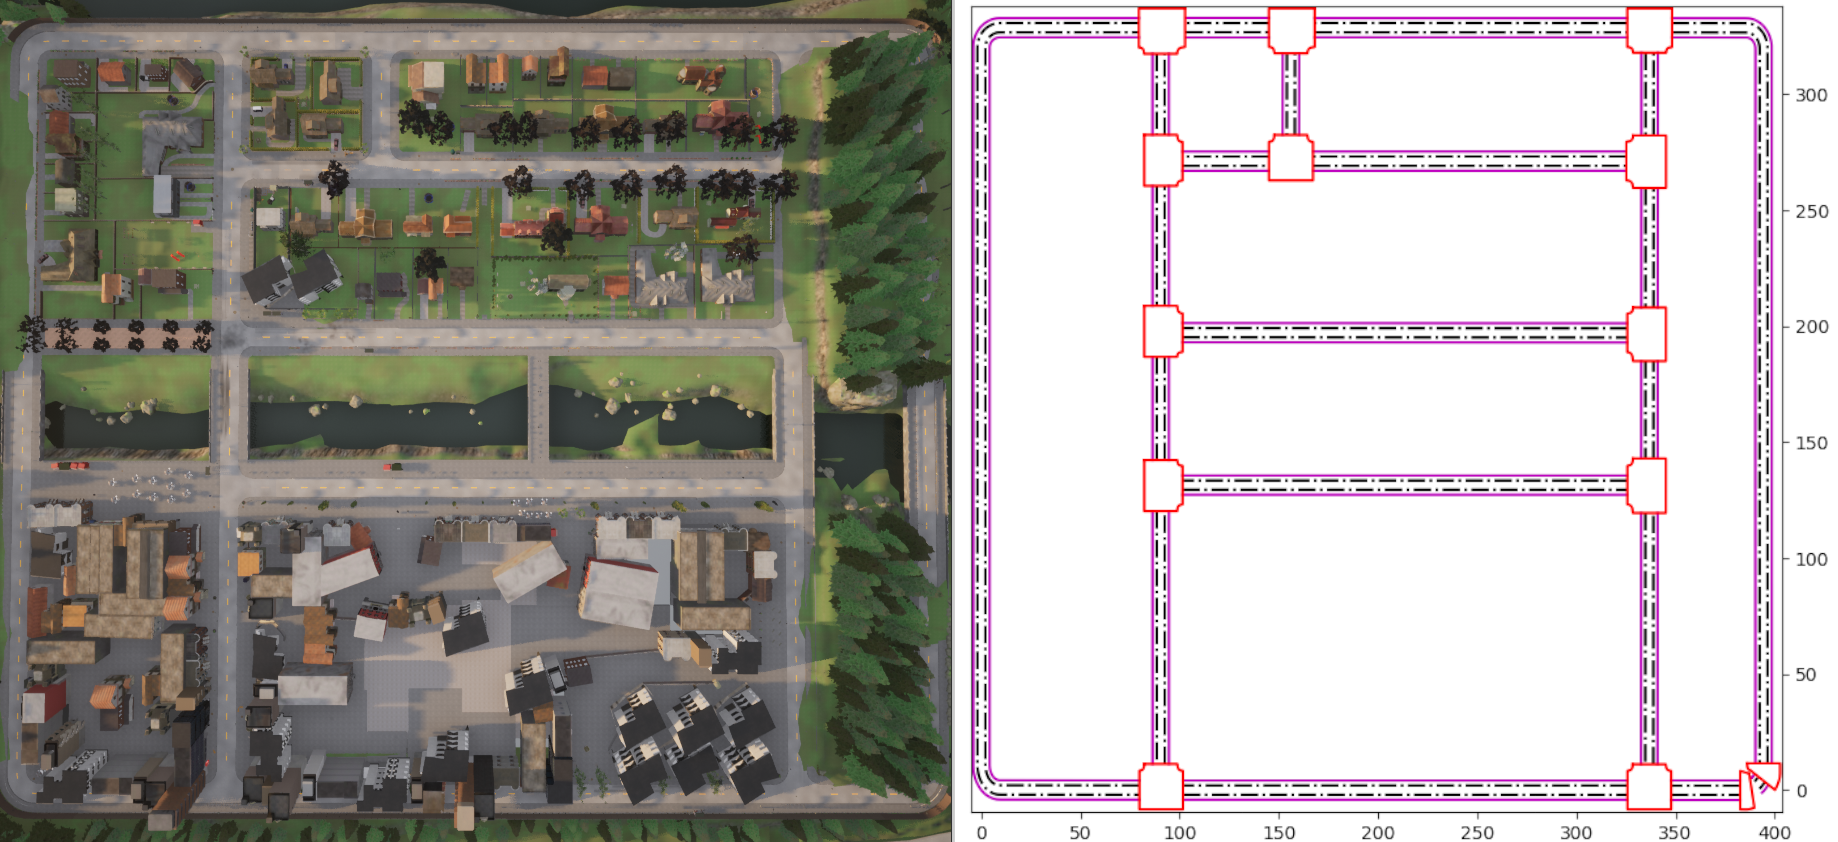
\includegraphics[width=1.0\textwidth]{chapter2/fig_town_map.png}
    \caption{The illustration of the road map in the simulator.}
    \label{fig:town_map}
\end{figure*}

The scheduling of model uploading in a vehicular federated learning system is considered, which consists of $M$ {\IAVs} deployed with multi-modal sensors.
Denote the set of {\IAVs} as $\carSet = \set{1, \dots, M}$.
Each {\IAV} collects the sensing data for the cooperative training of a deep neural network, e.g., SECOND \cite{SECOND}, in a federated learning manner \cite{FedAvg}.
This is one of the typical machine learning scenario in the application of autonomous driving as elaborated in \cite{icra2021-hong}.
In each training iteration, all the {\IAVs} first train their local models and then upload the trained models to an edge server for model aggregation via cellular uplink.
The aggregated model is then broadcast to the {\IAVs} for local training of next iteration until the convergence.
We particularly consider the uplink transmission scheduling in one iteration, where the {\IAVs}' mobility is exploited to save the transmission energy and suppress the model uploading time.

As an example illustrated in \figurename~\ref{fig:town_map}, $M$ {\IAVs} are distributed at different positions of a road network.
They are moving along predetermined routes respectively, but their velocities are time-varying and random.
The route of the $m$-th {\IAV} ($\forall m\in\carSet$) is quantized into a sequence of waypoints denoted as
\begin{align*}
    \tjSet_{m} \define \Paren{ \vec{w}_{m,1}, \dots, \vec{w}_{m,|\tjSet_{m}|} },
\end{align*}
where $\vec{w}_{m,i} \in \domR^2$ denotes the coordinates of the $i$-th waypoint,
$|\tjSet_m|$ denotes the cardinality of $\tjSet_m$.

The system time is organized by time slots, each with a duration of $T_s$ seconds.
In the $t$-th time slot, the location of the $m$-th {\IAV} is denoted as $\vec{d}_{m,t} \in \tjSet_{m}$, and the trajectory of the $m$-th {\IAV} is represented by its locations of the {\IAV} in all the time slots, denoted as
\begin{align*}
    \vec{L}_{m} \define \Paren{ \vec{d}_{m,1}, \vec{d}_{m,2}, \dots }.
\end{align*}
We approximate the trajectories of all {\IAVs} $\set{ \vec{L}_{m} | \forall m\in\carSet }$ as time-invariant Markov chains with the transition matrices
$\set{ \TransD_{m} \in \domR^{|\tjSet_{m}| \times |\tjSet_{m}|} | \forall m\in\carSet }$, where $\vec{D}_{m}$ represents the transition matrix of the $m$-th {\IAV}.
The entries of transition matrix $\TransD_{m}$ ($\forall m\in\carSet$) are defined as follows:
\footnote{
    A sufficient number of waypoints is selected for each route, such that the last waypoint is never reached at the end of the model uploading.
    For example, the uploading of the $m$-th {\IAV} always completes before arriving at the waypoint $\vec{w}_{m,|\tjSet_m|}$.
}
\begin{align}
     \Paren{\TransD_{m}}_{i,j} \define \Pr\Bracket{ \vec{w}_{m,j} | \vec{w}_{m,i} }, \forall i,j.
    \label{eqn:trans_mat}
\end{align}

Without loss of generality, the local model training and uploading of the considered iteration starts from the $1$-st time slot.
Due to the heterogeneous computation capabilities of the {\IAVs}, the local training time of the {\IAVs} may be different.
It is assumed that the local training time of the $m$-th {\IAV} is $T_{\text{comp},m}$, and the model consists of $U$ information bits.
Hence, an uplink queue with $U$ information bits is established at the $m$-th {\IAV} since the $(T_{\text{comp},m}+1)$-th time slot.
The period from the $1$-st time slot to the time slot that all the {\IAVs} complete their model uploading is referred to as the \emph{scheduling period} in the remaining of this chapter.
Thus, the length of the scheduling period depends on the uplink transmission scheduling.

All the {\IAVs} are served via a BS with $Y$ distributed antenna units,
and the locations of the antenna units are denoted as $\vec{b}_1, \dots, \vec{b}_Y$, respectively.
Each {\IAV} delivers its local model to the closest antenna unit, such that the transmission energy can be saved.
The distance between the $m$-th {\IAV} and the receiving antenna unit in the $t$-th time slot is denoted as
\begin{align*}
    l_{m,t} = \min_{i=1,2,\dots,Y} \|\vec{d}_{m,t} - \vec{b}_i\|_2.
\end{align*}
In order to avoid the co-channel interference, the {\IAVs} access the BS in a time-division manner in each time slot. There is at most one {\IAV} in the uplink transmission at any time instance. Let $\gamma_{m,t}$ be the ratio of the $t$-th time slot allocated to the $m$-th {\IAV}, we have
\begin{align*}
    \gamma_{m,t} \geq 0~\forall m\in\carSet \text{,~and} \sum_{m\in\carSet} \gamma_{m,t} \leq 1.
\end{align*}

Let $\mu_{m,t}$ be the path-loss of the $m$-th {\IAV}'s uplink channel in the $t$-th time slot, we have
\begin{align*}
    \mu_{m,t} = \kappa \bracket{ \frac{ \sigma }{ l_{m,t} } }^{\epsilon},
    % \label{eqn:mu}
\end{align*}
where $\kappa$ is a constant related to antenna characteristics, $\sigma$ is reference distance of the antenna far field, $\epsilon$ is the path-loss exponent.
Hence, the uplink throughput of the $m$-th {\IAV} in the $t$-th time slot $r_{m,t}$ is represented as follows:
\begin{align}
    r_{m,t} = \gamma_{m,t} T_s B_0
    \mathbb{E}_{h_{m,t}} \Bracket{
        \log_{2}\Paren{ 1 + \frac{|h_{m,t}|^2 \mu_{m,t} p_{m,t}}{N_0} }
    },
    \label{eqn:vu}
\end{align}
where $h_{m,t}$ is the coefficient of small-scale fading, $N_0$ is the power of Gaussian noise, $B_0$ is the uplink bandwidth, $p_{m,t}$ is the transmission power of the $m$-th {\IAV}, the expectation is taken over the random small-scale fading.
In the above equation, the ergodic capacity is used since the time slot is significantly longer than the channel coherent time.
Moreover, the transmission power should satisfy the following peak power constraint:
\begin{align*}
    p_{m,t} \leq P_{\max}.
\end{align*}

Let $u_{m,t}$ ($\forall, m,t$) be the remaining number of information bits in the uplink queue of the $m$-th {\IAV} in the $t$-th time slot, the queue dynamics are given by
\begin{align*}
    u_{m,t+1} = \max\Paren{ u_{m,t} - r_{m,t}, 0 }.
\end{align*}
Hence, the number of slots in the scheduling period, denoted by $T$, can be expressed as
\begin{align}
    T = \arg\min_{t} \indicator\Bracket{ \sum_{m\in\carSet} u_{m,t} \neq 0 }.
\end{align}


%=================================================================================================%
%=================================================================================================%

\section{Problem Formulation}
\label{sec:chapter2-formulation}
We would like to minimize the uplink energy consumption and model uploading time by exploiting the mobility of the {\IAVs}.
Because of their trade-off relation, the weighted summation of average uplink energy and uploading time (scheduling period duration) is used as the optimization objective.
Due to the randomness of {\IAVs}' trajectories, the joint scheduling design of the whole scheduling period, i.e., the transmission power and time allocation of all time slots, is a stochastic optimization problem, which can be formulated as a finite-horizon MDP.
We first define the system state, scheduling action, policy, and the cost function as follows.

\begin{definition}[State, Action and Policy]
    \label{def:mdp}
    In the $t$-th time slot, the local system state of the $m$-th {\IAV} is defined as
    \begin{align}
        \Stat_{m,t} &\define \Paren{ u_{m,t}, \vec{d}_{m,t} }, \forall m\in\carSet.
    \end{align}
    The global system state of the $t$-the time slot is defined as the aggregation of local system states of all {\IAVs}, thus
    \begin{align}
        \Stat_t &\define \Brace{ \Stat_{1,t}, \dots, \Stat_{M,t} }.
    \end{align}

    The scheduling action in the $t$-th time slot $\vec{A}_{t}$ consists of the allocation of transmission time and throughput%
    \footnote{
        Given the transmission time $\gamma_{m,t}$ and transmission power $p_{m,t}$,
        the throughput of the $m$-th {\IAV} in the $t$-th time slot $r_{m,t}$ can be determined according to Equation \eqref{eqn:vu}.
        We choose the transmission time and throughput as the action for the elaboration convenience.
    }
    of all {\IAVs},
    \begin{align}
        \vec{A}_{t} \define \Brace{ \gamma_{m,t}, r_{m,t} | \forall m\in\carSet }.
    \end{align}
    A centralized scheduling policy in the $t$-th time slot $\Policy_{t}$ is a mapping from the global system state $\Stat_{t}$ to the scheduling action, thus,
    \begin{align}
        \Policy_{t}\paren{\Stat_t} &= \Paren{ \Policy^{\Gamma}_{t}(\Stat_t), \Policy^{R}_{t}(\Stat_t) },
    \end{align}
    where $\Policy^{\Gamma}_{t}: \Stat_{t} \to \set{\gamma_{m,t} | m\in\carSet}$ denotes the throughput allocation policy and $\Policy^{R}_{t}: \Stat_{t} \to \set{r_{m,t} | m\in\carSet}$ denotes the time allocation policy.
\end{definition}

Given the action of the $t$-th time slot, the state transition probability from the $t$-th time slot to the $(t+1)$-th one is given by
\begin{align}
    &\Pr\Bracket{ \Stat_{t+1} | \Stat_{t}, \vec{A}_{t} } =
    % \nonumber\\
        \prod_{m\in\carSet} \Pr\Bracket{ \vec{d}_{m,t+1} | \vec{d}_{m,t} }
        \cdot \indicator\Bracket{ u_{m,t+1}=u_{m,t}+r_{m,t} },
    \label{eqn:trans_prob}
\end{align}
where $\Pr\bracket{ \vec{d}_{m,t+1} | \vec{d}_{m,t} }$ denotes the transition probability of the $m$-th {\IAV}'s trajectory from the waypoint $\vec{d}_{m,t}  \in \tjSet_{m}$ to $\vec{d}_{m,t+1} \in \tjSet_{m}$.

% It can be observed that different policies leads to different amount of uplink throughput, transmission energy consumption of each time slot, and finally different model uploading time and total energy consumption.
The policy design aims to minimize a weighted summation of the average model uploading time of all {\IAVs} and the average transmission energy consumption.
To achieve this goal, we define the system cost of the $t$-th time slot ($\forall t$) as follows:
\begin{align}
    g_{t}\Paren{ \Stat_{t}, \mathbf{A}_t } =
        \indicator\Bracket{ \sum\limits_{m\in\carSet} u_{m,t} > 0} +
        \omega \sum_{m\in\carSet} { \gamma_{m,t} p_{m,t} },
    \label{eqn:func_g}
\end{align}
where the two items on the right-hand-side (RHS) count the costs of uploading time and energy consumption, respectively, and $\omega$ is the weight on the energy consumption.

Hence, the expected overall cost of the whole scheduling period can be written as
\begin{align*}
    \widebar{G}\Paren{ \Policy_1,\dots,\Policy_\T } \define \mathbb{E}_{ \Stat_1,\dots,\Stat_\T } \Bracket{ \sum_{t=1}^{\T} g_{t}\paren{ \Stat_t, \vec{A}_t } },
\end{align*}
where $\T$ denotes the maximum tolerable number of time slots in one scheduling period.
As a result, the scheduling problem can be written as
\begin{align}
    \textbf{P1: } &\min_{\Policy_1, \dots, \Policy_\T} \widebar{G}\Paren{ {\Policy_1,\dots,\Policy_\T} }
    \label{eqn:p1_eqn}
    \\
    &\text{s.t.~~~~}
    \gamma_{m,t} \geq 0, \forall t, m\in\carSet
    \label{eqn:p1_cons_second}
    \\
    &~~~~~~\sum_{m\in\carSet} \gamma_{m,t} \leq 1, \forall t
    \label{eqn:p1_cons_last}
    \\
    &~~~~\sum_{ t=T_{\text{comp},m}+1 }^{\T} r_{m,t} \geq U, \forall m\in\carSet
    \\
    &~~~~p_{m,t} \leq P_{\max}, \forall t, m\in\carSet.
    \label{eqn:p1_cons_first}
\end{align}

In order to solve the above finite-horizon MDP, we first introduce the following Bellman's equations:
\begin{align}
    V_{t}(\Stat_t) =& \min_{\Policy_{t}(\Stat_t)} \Brace{ g_{t}\Paren{ \Stat_t, \vec{A}_t } +
    \sum_{\Stat_{t+1}} \Pr\Bracket{ \Stat_{t+1} | \Stat_{t}, \vec{A}_t } \cdot V_{t+1}(\Stat_{t+1})
    }, t=1,\dots,T,
    \label{eqn:p1_blm}
\end{align}
where
\begin{align}
    V_{t}(\Stat_{t}) \define \min_{\Policy_{t},\dots,\Policy_{\T}}& \mathbb{E}_{\Stat_{t},\dots,\Stat_{\T}}
    \Bracket{
        \sum_{\tau=t}^{\T} g_{\tau}\paren{ \Stat_{\tau}, \vec{A}_{\tau} } | \Stat_{t}
    }.
    \label{eqn:p1_val}
\end{align}
As a remark notice that in finite-horizon MDP, the optimal value functions can be heterogeneous for different time slots.

Hence, the optimal time and throughput allocation policies can be obtained by solving the RHS of equation \eqref{eqn:p1_blm}.
However, the problem {\bf P1} is difficult to solve.
On one hand, the transition probability of {\IAVs}' trajectories in Equation (\ref{eqn:trans_prob}) for a particular road network is hard to measure in advance, unless extensive real experiments can be conducted on the road network beforehand.
On the other hand, the optimal value functions depend on the global system state, which grows exponentially with respect to the number of {\IAVs}.

Thus, it is infeasible to calculate the value functions for each global system state before the online scheduling.
In order to address the above issues, a data-driven decentralized solution framework, namely {\fwName}, is proposed.
Particularly, the {\fwName} simulator is first proposed in Section \ref{sec:chapter2-framework} to obtain the waypoint transition probabilities.
Then the {\fwName} optimizer is proposed in Section \ref{sec:chapter2-new_framework} to address to issue of computation complexity in a decentralized manner.

\begin{figure*}[htp!]
    \centering
    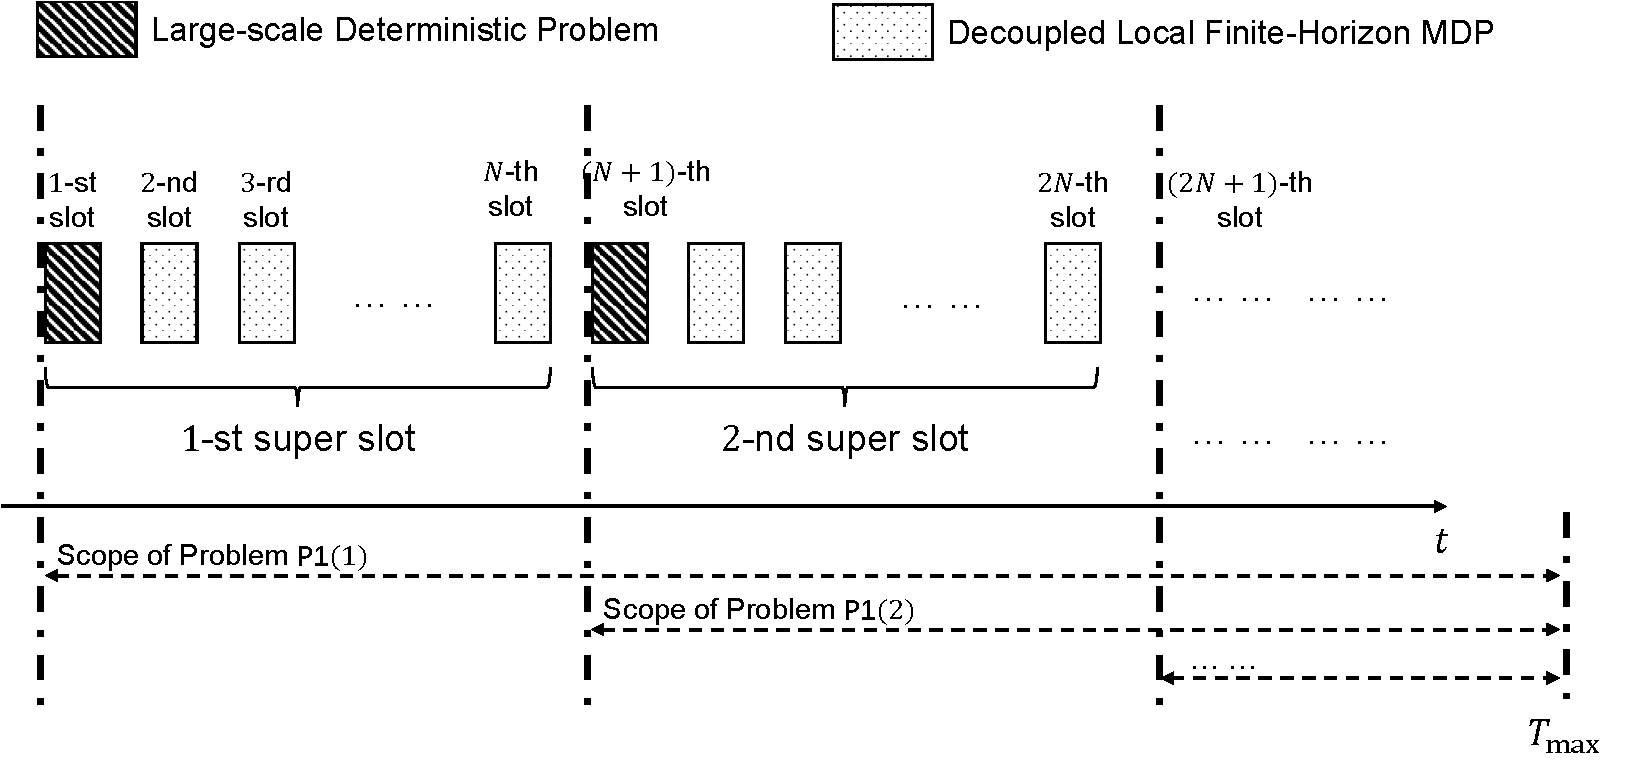
\includegraphics[width=1.0\textwidth]{chapter2/optimizer-framework.pdf}
    \caption{The illustration of the {\fwName} optimizer framework.}
    \label{fig:optimizer_framework}
\end{figure*}

\section{{\fwName} Simulator for Offline Transition Probability Training}
\label{sec:chapter2-framework}

The waypoint transition probabilities $\Pr\bracket{\vec{d}_{m,t+1}|\vec{d}_{m,t}}$ ($\forall m\in\carSet$) in \eqref{eqn:trans_prob} depend on the routes, the road topology, the microscopic traffic behaviors and etc, which are usually difficult to measure in advance.
A mismatching of the trajectories' statistics would lead to a biased estimation of the value function defined in \eqref{eqn:p1_val}, and degrade the performance of the optimized scheduling policy. To our best knowledge, there is currently no analytical model for the vehicles' trajectory prediction.
Therefore, we develop the {\fwName} simulator to simulate the trajectories of {\IAVs} for arbitrary traffic scenario, so that the waypoint transition probabilities $\Pr\bracket{\vec{d}_{m,t+1}|\vec{d}_{m,t}}$ can be trained in an offline manner.

The {\fwName} simulator integrates two well-known autonomous driving simulators, namely SUMO \cite{SUMO} and CARLA \cite{CARLA}.
CARLA is the open-source simulator based on Unreal Engine \cite{unrealengine}, which provides customized road topologies and vehicle types following the OpenDRIVE specification \cite{OpenDRIVE}.
On the other hand, SUMO provides the traffic management of vehicles with well-defined microscopic traffic flow model.
Based on them, the procedure to train the transition probabilities is given as follows.

\textbf{Road Topology and Traffic Initialization.} In order to simulate the random traffic on the particular scenario, we use CARLA to generate the target road map and leverage the program \emph{ActivityGen} provided by SUMO to generate random traffic demands according to the road map. The traffic demands can be customized by adjusting the following statistics: population distribution, working hours, car-holding rate, vehicular statistics and etc.
The study \cite{sumo-accuracy-mdpi} shows that the traffic flow generated by SUMO could match the traffic conditions of the real world on usual weekdays.

\textbf{Trajectory Dataset Generation.} Based on the above road map and traffic demands, the trajectories of all vehicles can be generated and recorded.
Let $\mathcal{X}_{m} $ be the set of vehicles running on the route of the $m$-th {\IAV} in all the simulation trials, and $$ \vec{x}^{(i)}_{m} = \Paren{ \vec{d}^{(i)}_{m,1}, \vec{d}^{(i)}_{m,2}, \dots }$$ be the trajectory of the $ i $-th vehicle in $\mathcal{X}_{m}$, where $\vec{d}^{(i)}_{m,t} \in \tjSet_{m}$ is the position in the $ t $-th time slot.

\textbf{Waypoint Transition Matrix Training.} Based on the trajectory dataset $ \{\vec{x}^{(i)}_{m}  | \forall i,m\} $, the waypoint transition matrices for all {\IAVs} $ \{\TransD_{m}| \forall m\} $ defined in \eqref{eqn:trans_mat} can be calculated as follows. 
\begin{align*}
    \Paren{\TransD_{m}}_{j,k} = 
        \frac{
            \sum_{t,i} \indicator\bracket{ \vec{d}^{(i)}_{t+1}=\vec{w}_{m,k}, \vec{d}^{(i)}_{t}=\vec{w}_{m,j} }
        }{
            \sum_{t,i}\sum_{l} \indicator \bracket{ \vec{d}^{(i)}_{t+1}=\vec{w}_{m,l}, \vec{d}^{(i)}_{t}=\vec{w}_{m,j} }
        }, \forall j,k.
\end{align*}
As a remark note that the trajectory dataset generation and waypoint transition matrix training are conducted in an offline manner before the uplink transmission, the {\fwName} simulator would have sufficient time to ensure a large number of trajectory samples. 

\begin{align}
    &\sum_{\tau=kN+1}^{T} g_{\tau}\Paren{
        \mathbb{E}_{\Stat_{\tau}} \Bracket{ \Stat_{\tau} | \Stat_{kN+1} }, \vec{A}_{\tau}
    }
    \nonumber\\
    \approx&~~T + \omega \sum_{\tau=kN+1}^{T} \sum_{m\in\carSet} \gamma_{m,\tau}
    2^\frac{r_{m,\tau}}{\gamma_{m,\tau}T_s B_0} 
    \times \xi_{m,\tau} \mathbb{E}_{\Stat_{\tau}} \Bracket{ l_{m,\tau}^{\epsilon}~|~\Stat_{kN+1} }
    \nonumber\\
    \define&~~F_k\Paren{ T, \mat{R}^{(k,T)}, \mat{\Gamma}^{(k,T)} }
    \label{eqn:fk}
\end{align}

\section{{\fwName} Optimizer: Online Decentralized Policy Optimization Framework}
\label{sec:chapter2-new_framework}

The joint policy optimization for the {\IAVs} in problem {\bf P1} suffers form the {\it curse of dimensionality}. This is because the transmission time and data rate allocation of each {\IAV} in each time slot depend on the global system state (aggregation of the states of all {\IAVs}), whose support grows exponentially with respect to the {\IAV} number.
It can be observed that if the transmission time allocation of all {\IAVs} $\{\gamma_{m,t}|\forall m,t\}$ is predetermined, the throughput allocation of each {\IAV} in all the time slots can be optimized without the consideration of other {\IAVs}' states.
However, fixing the transmission time allocation of all {\IAVs} before the model uploading would degrade the performance, as the transmission time allocation could not be adjusted according to the real-time positions and remaining information bits of all {\IAVs}.

In order to reduce the computation complexity and meanwhile maintain the performance gain of dynamic programming, a dynamic decoupling framework is proposed for the {\fwName} optimizer in this section. The framework is illustrated in \figurename~\ref{fig:optimizer_framework}, where every $N$ time slots is organized as a {\it super slot} and the online optimization consists of the following two time scales.
\begin{itemize}
    \item Super slot scale: the transmission time allocation of all {\IAVs} for the remaining time slots is periodically optimized at the beginning of each super slot. Such optimization will be approximated as a deterministic optimization problem based on the global system state at the beginning of each super slot.
    \item Slot scale: based on transmission time allocation, the optimization of throughput allocation policy of each {\IAV} for all the remaining time slots can be decoupled as a local finite-horizon MDP with tractable state space. The approximate expressions of local value functions will be derived, such that each {\IAV} can evaluate them and determine the throughput allocation in each slot without the effort of offline value iteration.
\end{itemize}

Without loss of generality, we consider the scheduling since the $k$-th super slot (from the $(kN+1)$-th time slot). The policy optimization of problem {\bf P1} for all the remaining time slots given the system state $\Stat_{kN+1}$ reduces to the following sub-problem:
\begin{align}
    \textbf{P1$(k)$:~~} &
    \min_{ \Policy_{kN+1}, \dots, \Policy_\T }
        \sum_{\tau=kN+1}^{\T}  \mathbb{E}_{\Stat_{\tau}} \Bracket{
            g_{\tau}\paren{ \Stat_{\tau}, \vec{A}_{\tau} } | \Stat_{kN+1}
        } \nonumber
    \\ \nonumber
    \text{s.t.~~} &\text{\eqref{eqn:p1_cons_second}, \eqref{eqn:p1_cons_last}, \eqref{eqn:p1_cons_first}},
    \\
    & \sum_{ \tau=\max\paren{kN+1,T_{\text{comp},m}} }^{ \T } r_{m,\tau} \geq {u}_{m,kN+1}, \forall m\in\carSet,
    \label{eqn:p1p_cons_last}
\end{align}
where the last constraint \eqref{eqn:p1p_cons_last} is to ensure all the data in the uplink queues of {\IAVs} should be delivered.


In the optimization of super slot scale, the average trajectories are used as the representatives to optimize the time slot allocation, such that the dynamic programming of problem \textbf{P1$(k)$} can be simplified to a deterministic optimization problem.
Note that
\begin{align}
    \sum_{\tau=kN+1}^{\T} g_{\tau}\Paren{
        \mathbb{E}_{\Stat_{\tau}}\Bracket{ \Stat_{\tau} | \Stat_{kN+1} }, \vec{A}_{\tau}
    }
    \label{eqn:cost_approx}
\end{align}
represents the system cost with the average trajectory
\begin{align}
    \Paren{
        \mathbb{E}\Bracket{ \vec{d}_{m,kN+1} | \vec{d}_{m,kN+1} },
        \dots,
        \mathbb{E}\Bracket{ \vec{d}_{m,T} | \vec{d}_{m,kN+1} }
    }
\end{align}
of the $m$-th {\IAV} ($\forall m\in\carSet$) since the $k$-th super slot. Approximating the objective by \eqref{eqn:cost_approx}, the policy optimization in problem \textbf{P1$(k)$} can be simplified into the following deterministic optimization of transmission time and throughput for the above average trajectories.
    \begin{align}
        \textbf{P2$(k)$:~} &
        ~~~\Paren{T^{(k,*)}, \mat{R}^{(k,*)}, \mat{\Gamma}^{(k,*)} }\nonumber \\
        & = \arg\min_{ T, \mat{R}^{(k,T)}, \mat{\Gamma}^{(k,T)} } F_k\Paren{ T, \mat{R}^{(k,T)}, \mat{\Gamma}^{(k,T)} }\nonumber
            \\
        &\text{s.t.~} \text{ \eqref{eqn:p1_cons_second}, \eqref{eqn:p1_cons_last}, \eqref{eqn:p1_cons_first},}
        \\
    & \sum_{ \tau=kN+1 }^{ T } r_{m,\tau} \geq {u}_{m,kN+1} \forall m\in\carSet, \label{eqn:constraint_T}
    \end{align}
where
$$
\mat{\Gamma}^{(k,T)} \define [ \gamma^{(k)}_{m,kN+\tau} ]_{1 \leq m \leq M, 1 \leq \tau \leq T-kN} \in \domR^{M \times (T-kN)}
$$
and
$$\mat{R}^{(k,T)} \define [ r^{(k)}_{m,kN+\tau}]_{1 \leq m \leq M, 1 \leq \tau \leq T-kN} \in \domR^{M \times (T-kN)}$$
are the aggregation matrices of time and throughput allocations of all the remaining time slots for the above average trajectories, respectively. $T$ denotes the number of slots in the scheduling period. $F_k(\cdot)$ is defined in Equation \eqref{eqn:fk}, where the high-SNR approximation on power consumption
\begin{align}
    p_{m,t} \approx \xi_{m,t} l_{m,t}^{\epsilon} 2^{\frac{ r_{m,t} }{ \gamma_{m,t} T_{s} B_0 }},
\end{align}
and $$\xi_{m,t} = \frac{N_0}{\kappa \sigma^\epsilon} 2^{-\mathbb{E}_{h_{m,t}}\bracket{\log_2{|h_{m,t}|^2}}}$$ is used.


The solution for the super slot scale optimization in problem \textbf{P2$(k)$} is discussed in Section \ref{sec:chapter2-kernel-policy}.
Its solution is denoted as
$$\mat{\Gamma}^{(k,*)}=[\gamma^{(k,*)}_{m,\tau+kN}]_{1 \leq m \leq M, 1 \leq \tau \leq T^{(k,*)}-kN}$$
and
$$\mat{R}^{(k,*)}=[r^{(k,*)}_{m,\tau+kN}]_{1 \leq m \leq M, 1 \leq \tau \leq T^{(k,*)}-kN}.$$
Moreover, $$\set{ \vecG{\gamma}^{(k,*)}_{m,\tau} | \forall m\in\carSet, \tau=kN+1,\dots,(k+1)N }$$ are adopted as the time allocation of the $k$-th super slot.

\noindent{\bf Remark:} {\it In high SNR region, with the reference time $\mat{\Gamma}^{(k,*)}$ and throughput allocations $\mat{R}^{(k,*)}$, the system cost with the average trajectory equals the average system cost with random trajectories. Thus,
\begin{align*}
F_k &\Paren{ T^{(k,*)}, \mat{R}^{(k,*)}, \mat{\Gamma}^{(k,*)}} =
\sum_{\tau=kN+1}^{T^{(k,*)}} \mathbb{E}_{\Stat_{\tau}} \Bracket{
            g_{\tau}\paren{ \Stat_{\tau}, \gamma^{(k,*)}_{m,\tau}, r^{(k,*)}_{m,\tau}} | \Stat_{kN+1}
        }.
\end{align*}
This will be exploited to derive a non-trivial performance bound of the proposed algorithm.}

In the optimization of slot scale, with the reference time allocation $\mat{\Gamma}^{(k,*)}$ and optimized length of scheduling period $T^{(k,*)}$, the throughput allocation policies of {\IAVs} can be decoupled. We first define the following local throughput allocation policies for the $m$-th {\IAV} ($\forall m\in\carSet$):
\begin{align}
    \Policy^{R}_{m,t}( \Stat_{m,t} ) = r_{m,t},~t=kN+1,\dots,T^{(k,*)}.
\end{align}
Moreover, the local reward function of the $m$-th {\IAV} is defined as
\begin{align}
    g_{m,t}\Paren{ \Stat_{m,t}, \Policy^{R}_{m,t}(\Stat_{m,t}) } = \gamma^{(k,*)}_{m,t} p_{m,t}.
\end{align}
Then the optimization of the local throughput allocation policies for the $m$-th {\IAV} can be written as follows:
\begin{align}
    \textbf{P3$(k,m)$:~}
    &\min_{ \set{\Policy^{R}_{m,\tau} | \tau=kN+1,\dots,T^{(k,*)} } }
        \nonumber\\
        &\sum_{\tau=kN+1}^{T^{(k,*)}}
        \mathbb{E}_{\Stat_{m,\tau}} \Bracket{
            g_{m,\tau}\Paren{ \Stat_{m,\tau}, \Policy^{R}_{m,\tau}( \Stat_{m,\tau} ) }\nonumber
        }
    \\\nonumber
    &\text{s.t.~} \text{ \eqref{eqn:p1_cons_second}, \eqref{eqn:p1_cons_last}, \eqref{eqn:p1_cons_first}, } \nonumber\\
    & ~~~ \sum_{ \tau=\max\paren{kN+1,T_{\text{comp},m}} }^{ T^{(k,*)}} r_{m,\tau} \geq {u}_{m,kN+1}.
\end{align}

Note that the above problem \textbf{P3$(k,m)$} is a finite-horizon MDP based on the local system state, it can be optimized locally at the $m$-th {\IAV}. The analytical expressions to approximate its local value functions will be proposed based on the reference time $\mat{\Gamma}^{(k,*)}$ and throughput allocation $\mat{R}^{(k,*)}$. Hence, at the beginning of each slot in the $k$-th super slot, the $m$-th {\IAV} first evaluates the next slot's local value function, and then determines the throughput allocation action of the current slot  according to the current local system state. The solution will be discussed in Section \ref{sec:chapter2-local-policy}.


%=================================================================================================%
%=================================================================================================%


\section{Global Super-Slot-Scale Optimization}
\label{sec:chapter2-kernel-policy}
The problem P2$(k)$ could be of a large scale when the number of remaining time slots is large. In this section, a large-scale optimization method is proposed.
Note that the time and throughput allocation ($\mat{\Gamma}^{(k,T)}, \mat{R}^{(k,T)}$) and scheduling period length $T$ are continuous and discrete, respectively, they can be optimized respectively. The optimization of P2$(k)$ given scheduling period length $T$ can be written as follows:
\begin{align}
    \textbf{P2$'(k,T)$:~}
    \min_{ \mat{R}^{(k,T)}, \mat{\Gamma}^{(k,T)} } &F_k\paren{ T, \mat{R}^{(k,T)}, \mat{\Gamma}^{(k,T)} }
    \\\nonumber
    \text{s.t.~} & \text{ \eqref{eqn:p1_cons_second}, \eqref{eqn:p1_cons_last}, \eqref{eqn:p1_cons_first}, \eqref{eqn:constraint_T} }.
\end{align}
Although the problem \textbf{P2$'(k,T)$} is convex, the conventional algorithms may not be applied due to huge complexity.
For example, the Newton interior method is of exponential computational complexity in the worst case \cite{monteiro1994}, which might be impractical for large $T$.
To address this issue, an acceleration gradient projection method \cite{Nesterov83} is adopted with convergence rate of $O(1/k^2)$ and computational complexity $O(k (M\T)^2)$, where $k$ denotes the number of iterations.

Let $\mat{R}^{(k,T)}_{0}, \mat{\Gamma}^{(k,T)}_{0}$ be an initial feasible solution satisfying the constraints \eqref{eqn:p1_cons_second}, \eqref{eqn:p1_cons_last}, \eqref{eqn:p1_cons_first}, and \eqref{eqn:constraint_T}.
Moreover, define
$$\mat{R}^{(k,T)}_{1}=\mat{R}^{(k,T)}_{0}, ~~\mat{\Gamma}^{(k,T)}_{1}=\mat{\Gamma}^{(k,T)}_{0}.$$
The problem \textbf{P2$'(k,T)$} can be solved by conducting the following two steps iteratively until convergence. 

\textbf{Step 1: Acceleration Point Calculation.}
In the $i$-th iteration ($i=1,2,3,\dots$), the acceleration points, denoted as $\widetilde{\mat{R}}^{(k,T)}_{i}$ and $\widetilde{\mat{\Gamma}}^{(k,T)}_{i}$, are chosen as the following linear combination of $(\mat{R}^{(k,T)}_{i}, \mat{R}^{(k,T)}_{i-1})$ and $(\mat{\Gamma}^{(k,T)}_{i}, \mat{\Gamma}^{(k,T)}_{i-1})$, respectively:
\begin{eqnarray*}
    &\widetilde{\mat{R}}^{(k,T)}_{i} &= \mat{R}^{(k,T)}_{i} + \frac{c_{i-1}-1}{c_{i}} \Paren{
        \mat{R}^{(k,T)}_{i} - \mat{R}^{(k,T)}_{i-1}
    }\nonumber
    \\
    &\widetilde{\mat{\Gamma}}^{(k,T)}_{i} &= \mat{\Gamma}^{(k,T)}_{i} + \frac{c_{i-1}-1}{c_{i}}  \Paren{
        \mat{\Gamma}^{(k,T)}_{i} - \mat{\Gamma}^{(k,T)}_{i-1} 
    },\nonumber
\end{eqnarray*}
where
\begin{align*}
    c_{0} = 1, c_{i} = \frac{1}{2} \Paren{ 1+\sqrt{ 1+4(c_{i-1})^2 } }.
\end{align*}

\textbf{Step 2: Update and Projection.}
Given the acceleration points, we define
$$\widebar{\mat{R}}^{(k,T)}_{i} = \widetilde{\mat{R}}^{(k,T)}_{i} - \eta \frac{\partial{F_k}}{\partial \mat{R}^{(k,T)}} \bigg|_{\widetilde{\mat{R}}^{(k,T)}_{i}}$$
and
$$\widebar{\mat{\Gamma}}^{(k,T)}_{i} = \widetilde{\mat{\Gamma}}^{(k,T)}_{i} - \eta \frac{\partial{F_k}}{\partial \mat{\Gamma}^{(k,T)}} \bigg|_{\widetilde{\mat{\Gamma}}^{(k,T)}_{i}}$$
where
\begin{align*}
    \frac{\partial{F_k}}{\partial \mat{R}^{(k,T)}} = \Bracket{
        &\xi_{m,\tau+kN} \mathbb{E}\bracket{ l_{m,\tau+kN}^{\epsilon} } \cdot
        2^{ \frac{r_{m,\tau+kN}}{\gamma_{m,\tau+kN} T_s B_0} }
        \nonumber\\
        &~~~~~~~~~~~~~~~~\cdot \paren{ \frac{\ln{2}}{T_s B_0} }
    }_{1 \leq m \leq M, 1 \leq \tau \leq T-kN},
    \\
    \frac{\partial{F_k}}{\partial \mat{\Gamma}^{(k,T)}} = \Bracket{
        &\xi_{m,\tau+kN} \mathbb{E}\bracket{ l_{m,\tau+kN}^{\epsilon} }
        \cdot 2^{ \frac{r_{m,\tau+kN}}{\gamma_{m,\tau+kN} T_s B_0} }
        \nonumber\\
        &\cdot \paren{1 - \frac{\ln{2}}{T_s B_0} \frac{r_{m,\tau+kN}}{\gamma_{m,\tau+kN}}}
    }_{1 \leq m \leq M, 1 \leq \tau \leq T-kN},
\end{align*}
 and $\eta$ is the constant gradient step size. Then the time and throughput allocations of the $i$-th iteration are updated as
\begin{align}
    \Paren{
        \mat{R}^{(k,T)}_{i+1}, &\mat{\Gamma}^{(k,T)}_{i+1}
    } = \mathcal{P}_{\C}\Paren{ \widebar{\mat{R}}^{(k,T)}_{i}, \widebar{\mat{\Gamma}}^{(k,T)}_{i} },
    \label{eqn:update_projection}
\end{align}
where $\mathcal{P}_{\C}$ denotes the projection of the matrix
$\widebar{\mat{R}}^{(k,T)}_{i}$ and $\widebar{\mat{\Gamma}}^{(k,T)}_{i}$
onto the constraint space $\C$ confined by equations \eqref{eqn:p1_cons_second}, \eqref{eqn:p1_cons_last}, \eqref{eqn:p1_cons_first} and \eqref{eqn:constraint_T}.

Specifically, let $\widebar{\gamma}^{(k,i)}_{m,\tau}$ and $\widebar{r}^{(k,i)}_{m,\tau}$ be the $(m,\tau)$-th entries of the matrices $\widebar{\mat{\Gamma}}^{(k,T)}_{i}$ and $\widebar{\mat{R}}^{(k,T)}_{i}$, respectively, the projection in Equation \eqref{eqn:update_projection} is equivalent to the following minimization problem:
\begin{align}
    \Paren{ \mat{R}^{(k,T)}_{i+1}, \mat{\Gamma}^{(k,T)}_{i+1} }
    = &\arg\min_{ \paren{ \mat{R},\mat{\Gamma} } \in \C }
            \nonumber\\
            &
            \sum_{m\in\carSet} \sum_{\tau=kN+1}^{T}
            \paren{ \widebar{\gamma}^{(k,i)}_{m,\tau} - \gamma_{m,\tau} }^{2} +
            \paren{ \widebar{r}^{(k,i)}_{m,\tau} - r_{m,\tau} }^{2}.
    \label{eqn:simplex_projection}
\end{align}
According to the proposition 2 of \cite{fast-projection}, the solution to the above projection problem is summarized in the following lemma.
\begin{lemma}[Alternative Projection Onto Simplex and Hyperplane]
    Let $\set{ \bar{\gamma}^{(m)}_{\tau} | \forall m\in\carSet }$ denote the descent sorting of $\set{ \bar{\gamma}^{(k,i)}_{m,\tau} | \forall m\in\carSet }$ in the $\tau$-th time slot ($\tau=kN+1,\dots,T$)
    ,
    and
    $\set{ \bar{r}^{(\tau)}_{m} | \tau=1,2,\dots,T-kN }$ denote the descent sorting of $\set{\bar{r}^{(k,i)}_{m,\tau} | \tau=kN+1,\dots,T}$ for the $m$-th {\IAV}.
    Thus,
    $\bar{\gamma}^{(1)}_{\tau} \geq \dots \geq \bar{\gamma}^{(M)}_{\tau}$ and $\bar{r}^{(1)}_{m} \geq \dots \geq \bar{r}^{(T-kN)}_{m}$.
    The solution of Equation \eqref{eqn:simplex_projection} is given by
    $\mat{\Gamma}^{(k,T)}_{i+1} = [\gamma^{(k,i+1)}_{m,kN+\tau}]_{1 \leq m \leq M, 1 \leq \tau \leq T-kN}$ and $\mat{R}^{(k,T)}_{i+1} = [r^{(k,i+1)}_{m,kN+\tau}]_{1 \leq m \leq M, 1 \leq \tau \leq T-kN}$.
    Moreover,
    \begin{align}
        \gamma^{(k,i+1)}_{m,\tau} = \Bracket{ \widebar{\gamma}^{(k,i)}_{m,\tau} &- \frac{\sum_{j=1}^{m'}\bar{\gamma}^{(j)}_{\tau} - 1}{m'} }^{+}
        \\
        r^{(k,i+1)}_{m,\tau} = \min\Paren{
            \Bracket{ \widebar{r}^{(k,i)}_{m,\tau} &- \frac{\sum_{j=1}^{\tau'}u_{m,t} - \bar{r}^{(j)}_{m}}{\tau'} }^{+},
            \nonumber\\
            &T_s B_0 \log_2\paren{ \frac{P_{\max}}{ \xi_{m,\tau} \mathbb{E}[l^{\epsilon}_{m,\tau}]}} \gamma^{(k,i+1)}_{m,\tau}
        }
    \end{align}
    where
    $$m' = \max_{m} \set{m: {\sum_{j=1}^{m} \bar{\gamma}^{(j)}_{\tau} - 1 } <{m} \bar{\gamma}^{(m)}_{\tau}},$$ 
    $$\tau' = \max_{\tau} \set{\tau: {\sum_{j=1}^{\tau} u_{m,t} - \bar{r}^{(j)}_{m}} <{\tau} \bar{r}^{(\tau)}_{m}}.$$
\end{lemma}

Denote ${\mat{\Gamma}^{(k,T,*)}}$ and ${\mat{R}^{(k,T,*)}}$ as the optimized time and throughput allocations of problem \textbf{P2$'(k,T)$} after convergence, the optimization of scheduling period duration can be written as follows.
\begin{align}
    \textbf{P2$''(k)$:~} & \min_{T} F_{k}  \Paren{T, {\mat{\Gamma}^{(k,T,*)}}, {\mat{R}^{(k,T,*)}} }.
    \label{eqn:p2pp_k}
\end{align}
Note that the variable $T$ is an integer between $1$ and $\T$, a  bisection search algorithm is elaborated below to solve problem \textbf{P2$''(k)$}. Finally, the optimized scheduling period duration $T$ in problem \textbf{P2$''(k)$} is denoted as $T^{(k,*)}$, the corresponding optimized time and throughput allocations are denoted as $\mat{\Gamma}^{(k,*)}$ and  ${\mat{R}^{(k,*)}}$ respectively. 
\begin{algorithm}[ht]
    \caption{Bisection Search Algorithm for problem \textbf{P2$''(k)$}}\label{alg_bnb}
    \DontPrintSemicolon
    \KwOut{ $T^{(k,*)}$ }
    % \KwOut{$\{ { \gamma^{*}_{m,\tau} }, { r^{*}_{m,\tau} } | \forall m\in\carSet, \tau=kN+1,\dots,{T}^{*} \}$}
    $\tau_{l} \gets kN+1$, $\tau_{r} \gets \T$\;
     $w_{r} \gets \min F_{k}( \tau_{r}, \mat{R}_{r}, \mat{\Gamma}_{r} )$ by solving \textbf{P2$'( k,\tau_{r} )$}\;
    \While{ $\tau_{r} - \tau_{l} > 1$ }
    {
        $\tau_{mid} \gets \lfloor{ (\tau_{l} + \tau_{r})/2 }\rfloor$\;
        $w_{mid} \gets \min F_{k}( \tau_{mid}, \mat{R}_{mid}, \mat{\Gamma}_{mid} )$ by solving \textbf{P2$'( k,\tau_{mid} )$}\;
        \If{ $w_{r} - w_{mid} < 0$ }{
            $\tau_{l} \gets \tau_{mid}$\; %g(x)/energy domains, moves right
        }
        \Else{
            $\tau_{r} \gets \tau_{mid}$\; %f(x)/time domains, moves left
            $w_{r} \gets w_{mid}$\;
        }
    }
    \Return{ $T^{(k,*)} \gets \tau_{l}$ }\;
\end{algorithm}

\section{Local Slot-Scale Optimization}
\label{sec:chapter2-local-policy}

In this section, the low-complexity algorithm solving the problem \textbf{P3$(k,m)$} without the offline value iteration is elaborated. Note that the local system state of the $m$-th {\IAV} consists of $\Stat_{m,t} =  ( u_{m,t}, \vec{d}_{m,t} )$, the Bellman's equations of problem \textbf{P3$(k,m)$} are given below.
\begin{align*}
    V_{m,t} & \paren{  u_{m,t}, \vec{d}_{m,t} }=
    \min_{ r_{m,t} } \gamma^{(k,*)}_{m,t} p_{m,t} + \mathbb{E}_{ \vec{d}_{m,t+1} } V_{m,t+1}\paren{  u_{m,t}-r_{m,t}, \vec{d}_{m,t+1} },
\end{align*}
where the transmission power $p_{m,t}$ is a function of $\gamma^{(k,*)}_{m,t}$, $\vec{d}_{m,t}$ and $r_{m,t}$, and the local value function of the $m$-th {\IAV} in the $t$-th time slot is given by
\begin{align}
    V_{m,t} & (u_{m,t}, \vec{d}_{m,t}) \define 
    \min_{ \{\Policy^{R}_{m,t}|\forall t\} } \mathbb{E} \Bracket{ \sum_{\tau=t}^{T^{(k,*)}} g_{m,t}(u_{m,t}, \vec{d}_{m,t}, \Policy^{R}_{m,t}) }.
\end{align}
For the notation convenience, we define
\begin{align}
    \widetilde{V}_{m,t+1}\paren{u_{m,t+1}, \vec{d}_{m,t}} = \mathbb{E}_{ \vec{d}_{m,t+1} | \vec{d}_{m,t} } V_{m,t+1}\paren{  u_{m,t+1}, \vec{d}_{m,t+1} }.
 \label{eqn:local_valfn_alt}
\end{align}
Hence, given the local value function and local system state, the optimal throughput allocation of the $m$-th {\IAV} in the $t_i$-th time slot, where  $t_i = kN + i$ and $i=1,2,\dots,N$, can be obtained via the following optimization problem.
\begin{align}
    \min_{ r_{m,t_i} } \gamma^{(k,*)}_{m,t_i} p_{m,t_i} (r_{m,t_i})+ \widetilde{V}_{m,t_i+1}\paren{u_{m,t_i}-r_{m,t_i}, \vec{d}_{m,t_i}}.
    \label{eqn:local_valfn}
\end{align}

Although the dimension of local value function is much less than the global optimization in Equation \eqref{eqn:p1_blm},
the complexity of evaluating local value functions $V_{m,t}  (u_{m,t}, \vec{d}_{m,t})$ ($\forall t, u_{m,t}, \vec{d}_{m,t}$) or equivalently $\widetilde{V}_{m,t}(\cdot)$ is still high. Therefore, we propose a novel method to approximate the local value functions with the analytical expressions based on the reference throughput allocation. 
Let
$$\paren{ r^{(k,i-1)}_{m,t_i}, r^{(k,i-1)}_{m,t_i+1}, \dots, r^{(k,i-1)}_{m,T^{(k,*)}} }$$
with 
\begin{align}
    \sum_{\tau=t_i}^{T^{(k,*)}} r^{(k,i-1)}_{m,\tau} = u_{m,t_i}
    \label{eqn:reference_constraint}
\end{align}
be the reference throughput allocation for all the remaining time slots in the optimization of the $t_i$-th time slot, and
\begin{align*}
    \slide{r}^{(k,i-1)}_{m} = \paren{ r^{(k,i-1)}_{m,t_i+1}, r^{(k,i-1)}_{m,t_i+2}, \dots, r^{(k,i-1)}_{m,T^{(k,*)}} }
\end{align*}
be the corresponding reference throughput allocation for the future time slots. The optimization in Equation \eqref{eqn:local_valfn} can be equivalently written as
\begin{align}
\textbf{P3$'(k,m,t_i)$:}& \min_{ \Delta r_{m,t_i} } \gamma^{(k,*)}_{m,t_i} p_{m,t_i} (r^{(k,i-1)}_{m,t_i}+\Delta r_{m,t_i}) \nonumber\\ 
 +~&\widetilde{V}_{m,t_i+1}\paren{u_{m,t_i}-r^{(k,i-1)}_{m,t_i}-\Delta r_{m,t_i}, \vec{d}_{m,t_i}}.  \label{eqn:local_valfn_delta}
 \\
 \text{s.t.~}& p_{m,t_i}( r^{(k,i-1)}_{m,t_i} + \Delta{r}_{m,t_i} ) \leq P_{\max}
\end{align}

\subsection{Local Value Function Approximation}
\label{subsec:chapter2-local_valfn_approx}

In this section, we approximate the expected local value function $\widetilde{V}_{m,t_i+1}\paren{\cdot}$ in Equation \eqref{eqn:local_valfn_delta} via the reference throughput allocations $\slide{r}^{(k,i-1)}_{m}$.
Let 
\begin{align}
    \widebar{G}_{m,t_i+1} & \paren{ \slide{r}^{(k,i-1)}_{m}, \vec{d}_{m,t_i} }
    \define
    \sum_{\tau=t_i+1}^{T^{(k,*)}}
    \mathbb{E}_{\vec{d}_{m,\tau}}\Bracket{
        \gamma^{(k,*)}_{m,\tau} p_{m,\tau}\paren{ r_{m,\tau}^{(k,i-1)}}
        ~|~\vec{d}_{m,t_i}
    }
\end{align}
denote the expected cost of $m$-th {\IAV} since the $(t_i+1)$-th time slot with the reference throughput allocations $\slide{r}^{(k,i)}_{m} $ given the current location $\vec{d}_{m,t_i}$, and
$$
\Delta{\slide{r}^{(k,i)}_{m}} = (\Delta{r}_{m,t_i+1},\dots,\Delta{r}_{m,T^{(k,*)}})
$$
be the adjustment on the reference throughput allocation.
We approximate the expected local value function $\widetilde{V}_{m,t_i+1}\paren{\cdot}$ in Equation \eqref{eqn:local_valfn_delta} as follows:
\begin{align}
    \widetilde{V}_{m,t_i+1} & ( u_{m,t_i} -r^{(k,i-1)}_{m,t_i} -\Delta{r}_{m,t_i}, \vec{d}_{m,t_i} )  \approx
    \nonumber\\
     \min_{\Delta{\slide{r}^{(k,i)}_{m}}} & ~~~\widebar{G}_{m,t_i+1}\Paren{ \slide{r}^{(k,i-1)}_{m} + \Delta{\slide{r}^{(k,i)}_{m}}, \vec{d}_{m,t_i} }
    \nonumber\\
    \text{s.t.~} & ~~~ \sum_{\tau=t_i+1}^{T^{(k,*)}} \Delta{r}_{m,\tau} = \Delta{r}_{m,t_i}
    \nonumber\\
    & ~~~ \Delta{r}_{m,t_i} \times \Delta{r}_{m,\tau} \geq 0, \forall \tau = {t_i+1},\dots, T^{(k,*)}. \nonumber
\end{align}
The above first constraint is to ensure that the total number of transmission bits is $u_{m,t_i}$, and the second constraint is to limit the search space of $\Delta{\slide{r}^{(k,i)}_{m}}$. Moreover, we have the following conclusion on its asymptotic optimal solution.

\begin{lemma}
    \label{lemma:local_rate_opt}
    Define the following indexes of time slots:
     \begin{align}
        \hat{\tau}_{m} &= \arg\max_{\tau} \mathbb{E}\Bracket{ l_{m,\tau}^{\epsilon}~|~\vec{d}_{m,t_i} }
                          \cdot 2^{\frac{r^{(k,i)}_{m,\tau}}{T_s B_0 \gamma^{(k,*)}_{m,\tau}}},
        \\
        \breve{\tau}_{m} &= \arg\min_{\tau} \mathbb{E}\Bracket{ l_{m,\tau}^{\epsilon}~|~\vec{d}_{m,t_i} }
                          \cdot 2^{\frac{r^{(k,i)}_{m,\tau}}{T_s B_0 \gamma^{(k,*)}_{m,\tau}}}.
    \end{align}   
    For sufficiently small $\Delta{r}_{m,t_i}$, the following solution is asymptotically optimal:
    \begin{itemize}
        \item If $\Delta{r}_{m,t_i} > 0$, all the entries of $\Delta{\slide{r}^{(k,i)}_{m}}$ is $0$ except that $\Delta{r}_{m,\hat{\tau}_{m}} = \Delta{r}_{m,t_i}$;
        \item If $\Delta{r}_{m,t_i} < 0$, all the entries of $\Delta{\slide{r}^{(k,i)}_{m}}$ is $0$ except that $\Delta{r}_{m,\breve{\tau}_{m}} = \Delta{r}_{m,t_i}$;
    \end{itemize}
\end{lemma}
\begin{proof}
    The original optimization problem is convex, and we discuss the solution depending on the sign of $\Delta{r}_{m,t_i}$ in the following two cases.

    In the case when $\Delta{r}_{m,t_i} \leq 0$, we have $\Delta{r}_{m,\tau} \geq 0$ ($\tau=t_i+1, \dots, T^{(k,*)}$).
    Therefore, let $\lambda \in \domR_+$ and $\vecG{\mu} \in \domR^{(T^{(k,*)}-t_i)}_+$ denote the Lagrangian multipliers, the corresponding Lagrangian function of the convex optimization problem is given as follows:
    \begin{align*}
        L( \Delta{\slide{r}}^{(k,i)}_{m}, \lambda, \vecG{\mu} ) =
        &\sum_{\tau=t_i+1}^{T^{(k,*)}} \gamma^{(k,*)}_{m,\tau} p_{m,\tau}( r^{(k,i)}_{m,\tau} - \Delta{r}_{m,\tau} )
        \nonumber\\
        &+ \lambda \Paren{ \sum_{\tau=t_i+1}^{T^{(k,*)}} \Delta{r}_{m,\tau} - \Delta{r}_{m,t_i} }
        - \sum_{j=1}^{T^{(k,*)}-t_i} \mu_{j} \Delta{r}_{m,t_i+j}.
    \end{align*}

    The Karush-Kuhn-Tucker (KKT) conditions for the original convex optimization problem are:
    \begin{enumerate}
        \item primal constraints: $\sum_{\tau=t_i+1}^{T^{(k,*)}} \Delta{r}_{m,\tau} - \Delta{r}_{m,t_i} \leq 0$, $\Delta{\slide{r}}^{(k,i)}_{m} \vecG{\mu}^T = 0$;
        \item dual constraints: $\lambda \geq 0$;
        \item complementary slackness:
        $$
        \lambda (\sum_{\tau=t_i+1}^{T^{(k,*)}} \Delta{r}_{m,\tau} - \Delta{r}_{m,t_i}) = 0;
        $$
        \item stationarity:
        $$
        \nabla_{\Delta{\slide{r}}^{(k,i)}_{m}} L( \Delta{\slide{r}}^{(k,i)}_{m}, \lambda, \vec{\mu} )
        = \vec{0},
        $$
        i.e.,
        $$
        - \frac{\ln{2}}{T_s B_0} \mathbb{E}[l^{\epsilon}_{m,t_i+j}] \cdot 2^{\frac{r^{(k,i)}_{m,t_i+j} - \Delta{r}_{m,t_i+j}}{T_s B_0 \gamma^{(k,*)}_{m,t_i+j}}} + \lambda - \mu_j = 0,
        \forall j.
        $$
    \end{enumerate}

    Notice that $\Delta{\slide{r}}^{(k,i)}_{m} \vecG{\mu}^T = 0$ is always true for optimal solution, we have the following statements:
    \begin{itemize}
        \item if $\mu_j > 0$, then $\Delta{r}_{m,t_i+j} = 0$, which implies
        $$
        \lambda < \frac{\ln{2}}{T_s B_0} \mathbb{E}[l^{\epsilon}_{m,t_i+j}] \cdot 2^{\frac{r^{(k,i)}_{m,t_i+j}}{T_s B_0 \gamma^{(k,*)}_{m,t_i+j}}}.
        $$
        For the corresponding contrapositive statement, we have: if $\lambda \geq \frac{\ln{2}}{T_s B_0} \mathbb{E}[l^{\epsilon}_{m,t_i+j}] \cdot 2^{\frac{r^{(k,i)}_{m,t_i+j}}{T_s B_0 \gamma^{(k,*)}_{m,t_i+j}}}$, then $\Delta{r}_{m,t_i+j} > 0$.
        \item if $\mu_j = 0$, then $\Delta{r}_{m,t_i+j} \geq 0$, and we have
        $$
        \Delta{r}_{m,\tau} = - r^{(k,i)}_{m,\tau} + T_s B_0 \gamma^{(k,*)}_{m,\tau} \log_2{\frac{T_s B_0 \lambda}{\ln{2} \mathbb{E}[l^{\epsilon}_{m,\tau}]}}.
        $$
    \end{itemize}

    Therefore, for sufficiently small $\Delta{r}_{m,t_i}$, the index of non-zero rate allocation is the {\it largest} one satisfying the constraint w.r.t $\lambda$, i.e.,
    $$
    \hat{\tau}_{m} = \arg\max_{\tau} \mathbb{E}\Bracket{ l_{m,\tau}^{\epsilon}~|~\vec{d}_{m,t_i} }
                            \cdot 2^{\frac{r^{(k,i)}_{m,\tau}}{T_s B_0 \gamma^{(k,*)}_{m,\tau}}}.
    $$

    Similarly, in the case when $\Delta{r}_{m,t_i} \ge 0$, let $\Delta{\slide{r}}^{(k,i)'}_{m} = - \Delta{\slide{r}}_{m,t_i}$, we have the Lagrangian function $L'(\cdot)$ w.r.t $\Delta{\slide{r}}^{(k,i)'}_{m,t_i}$ as follows:
    \begin{align*}
        &L'( \Delta{\slide{r}}^{(k,i)'}_{m}, \lambda, \vecG{\mu} ) =
        \sum_{\tau=t_i+1}^{T^{(k,*)}} \gamma^{(k,*)}_{m,\tau} p_{m,\tau}( r^{(k,i)}_{m,\tau} + \Delta{r}'_{m,\tau} )
        \nonumber\\
        &- \lambda \Paren{ \sum_{\tau=t_i+1}^{T^{(k,*)}} \Delta{r}_{m,\tau} - \Delta{r}_{m,t_i} }
        - \sum_{j=1}^{T^{(k,*)}-t_i} \mu_{j} \Delta{r}_{m,t_i+j}.
    \end{align*}
    Therefore, the only difference compared to the analysis in previous case exists in stationarity constraint, where
    $$
    \frac{\ln{2}}{T_s B_0} \mathbb{E}[l^{\epsilon}_{m,t_i+j}] \cdot 2^{\frac{r^{(k,i)}_{m,t_i+j} - \Delta{r}'_{m,t_i+j}}{T_s B_0 \gamma^{(k,*)}_{m,t_i+j}}} + \lambda - \mu_j = 0,
        \forall j.
    $$
    For sufficiently small $\Delta{r}_{m,t_i}$, the index of non-zeros rate allocation is the {\it smallest} one, i.e.,
    $$
    \breve{\tau}_{m} = \arg\min_{\tau} \mathbb{E}\Bracket{ l_{m,\tau}^{\epsilon}~|~\vec{d}_{m,t_i} }
                            \cdot 2^{\frac{r^{(k,i)}_{m,\tau}}{T_s B_0 \gamma^{(k,*)}_{m,\tau}}}.
    $$
\end{proof}
As a result, the expected approximate value function can be approximated as follows.
\begin{align}
    &\widetilde{V}_{m,t_i+1}\paren{ u_{m,t_i}-r^{(k,i-1)}_{m,t_i}-\Delta{r}_{m,t_i}, \vec{d}_{m,t_i} }
    \nonumber\\
    &\approx
    \begin{cases}
        \widebar{G}_{m,t_i+1}\paren{ \slide{r}^{(k,i-1)}_{m} + \vec{e}_{\hat{\tau}_{m}} \Delta{r}_{m,t_i}, \vec{d}_{m,t_i} }, & \Delta{r}_{m,t_i} > 0
        \\
        \widebar{G}_{m,t_i+1}\paren{ \slide{r}^{(k,i-1)}_{m} + \vec{e}_{\breve{\tau}_{m}} \Delta{r}_{m,t_i}, \vec{d}_{m,t_i} }, & \Delta{r}_{m,t_i} < 0
    \end{cases}. \label{eqn:local-value-app}
\end{align}
In the above expressions, $\vec{e}_{\tau}$ denotes the vector whose $\tau$-th dimension is one and other dimensions are zero.

\subsection{Online Scheduling}
\label{subsec:chapter2-local_opt}
With the local value function approximation in the previous section, the local throughput allocation of the $m$-th {\IAV} in the $t_i$-th slot can be determined by solving problem \textbf{P3$'(k,m,t_i)$}. We first introduce the following conclusion.
\begin{lemma}
    \label{lemma:local_approx_solution}
    With the approximation of local value function in Equation \eqref{eqn:local-value-app}, the optimal solution of problem \textbf{P3$'(k,m,t_i)$} is within the set $\{f_{m,t_i}(\hat{\tau}_m),f_{m,t_i}(\breve{\tau}_m) \}$, where
    \begin{align}
        f_{m,t_i}(\tau_m) \define
        \min\Paren{
            &\frac{
                T_s B_0 \gamma^{(k,*)}_{m,t_i} \gamma^{(k,*)}_{m,\tau} \paren{ \log_2{ \mathbb{E}[l^{\epsilon}_{m,\tau_m}] } - \log_2{l^{\epsilon}_{m,t_i}} } 
            }{
                \gamma^{(k,*)}_{m,t_i} + \gamma^{(k,*)}_{m,\tau_m}
            }
            \nonumber\\
            &+\frac{
                r^{(k,*)}_{m,\tau_m}\gamma^{(k,*)}_{m,t_i} - r^{(k,*)}_{m,t_i}\gamma^{(k,*)}_{m,\tau_m} 
            }{
                \gamma^{(k,*)}_{m,t_i} + \gamma^{(k,*)}_{m,\tau_m}
            },
            \Delta{r}^{\max}_{m,t_i}
        },
    \end{align}
    where $p_{m,t_i}( r^{(k,i-1)}_{m,t_i} + \Delta{r}^{\max}_{m,t_i} ) = P_{\max}$.
\end{lemma}
\begin{proof}
    Note that given the fixed solution $\tau$, the corresponding optimal rate allocation is given as follows:
    \begin{align*}
        \min_{ \Delta{r}_{m,t_i} } &\gamma^{(k,*)}_{m,t_i} p_{m,t_i}( r^{(k,i)}_{m,t_i} + \Delta{r}_{m,t_i} )
            + \gamma^{(k,*)}_{m,\tau} p_{m,\tau}( r^{(k,i)}_{m,\tau} - \Delta{r}_{m,t_i} )
    \end{align*}
    The solution to the above optimization problem is easy to obtain by taking the derivative w.r.t $\Delta{r}_{m,t_i}$ and setting it to zero, i.e.,
    $$
    \frac{\ln{2}}{T_s B_0} l^{\epsilon}_{m,t_i} 2^{\frac{r^{(k,i)}_{m,t_i} + \Delta{r}_{m,t_i}}{T_s B_0 \gamma^{(k,*)}_{m,t_i}}}
    + \frac{\ln{2}}{T_s B_0} \mathbb{E}[l^{\epsilon}_{m,\tau}] 2^{\frac{r^{(k,i)}_{m,\tau} - \Delta{r}_{m,t_i}}{T_s B_0 \gamma^{(k,*)}_{m,\tau}}} = 0,
    $$
    and the solution is
    \begin{align*}
        \Delta{r}_{m,t_i} =
        &\frac{
            T_s B_0 \gamma^{(k,*)}_{m,t_i} \gamma^{(k,*)}_{m,\tau} \paren{ \log_2{ \mathbb{E}[l^{\epsilon}_{m,\tau}] } - \log_2{l^{\epsilon}_{m,t_i}} } 
        }{
            \gamma^{(k,*)}_{m,t_i} + \gamma^{(k,*)}_{m,\tau}
        }
        \nonumber\\
        &+ \frac{
            r^{(k,*)}_{m,\tau}\gamma^{(k,*)}_{m,t_i} - r^{(k,*)}_{m,t_i}\gamma^{(k,*)}_{m,\tau} 
        }{
            \gamma^{(k,*)}_{m,t_i} + \gamma^{(k,*)}_{m,\tau}
        }.
    \end{align*}
\end{proof}

Hence, the optimized throughput allocation of the $m$-th {\IAV} in the $t_i$-th slot is denoted by
\begin{align}
    r^{(k,i)}_{m,t_i} = r^{(k,i-1)}_{m,t_i}+f_{m,t_i}(\tau_m^*), \label{eqn:throughput}
\end{align}
where 
\begin{align}
    \tau_m^*=\arg \min_{ \tau_m\in \{\hat{\tau}_m,\breve{\tau}_m\} } &\gamma^{(k,*)}_{m,t_i} p_{m,t_i} (r^{(k,i-1)}_{m,t_i}+f_{m,t_i}(\tau_m)) \nonumber\\
 & + \widebar{G}_{m,t_i+1}\paren{ \slide{r}^{(k,i-1)}_{m} + \vec{e}_{\tau_{m}} f_{m,t_i}(\tau_m), \vec{d}_{m,t_i} }.
    \label{eqn:opt_tau}
\end{align}

\subsection{Proposed Policy and Performance Bound}
As a result of global super-slot-scale optimization and local slot-scale optimization, the proposed policy, denoted as $\Baseline$, is summarized below.
\begin{definition}[Proposed Policy $\Baseline$]
    \label{def:baseline}
    In the $t_i$-th time slot where $t_i=kN+i$ ($\forall k,i$),
    the transmission time allocation of {\IAVs} $[ \gamma^{\Baseline}_{m,t_i}]_m$ is obtained by solving problem \textbf{P2$(k)$} every super slot, and the uplink throughput allocation $[ r^{\Baseline}_{m,t_i}]_m$ is obtained from Equation \eqref{eqn:throughput} with the reference throughput allocation
    $\paren{ r^{(k,i-1)}_{m,t_i}, r^{(k,i-1)}_{m,t_i+1}, \dots, r^{(k,i-1)}_{m,T^{(k,*)}} }$.
    Hence,  $$\gamma^{\Baseline}_{m,t_i}=\gamma^{(k,*)}_{m,t_i} \mbox{ and } r^{\Baseline}_{m,t_i} = r^{(k,i)}_{m,t_i}, \ \forall m.$$
\end{definition}

Although arbitrary reference throughput allocation satisfying Equation \eqref{eqn:reference_constraint} can be used in the above approximation of local value function, the following initialization and iterative update of reference throughput allocation could lead to a non-trivial bound of the proposed algorithm. 
\begin{itemize}
    \item {\bf Initialization:} When $i=1$, 
    \begin{align}
        r^{(k,1)}_{m,\tau} = r^{(k,*)}_{m,\tau}, \forall \tau = t_{1}, \dots, T^{(k,*)}\nonumber,
    \end{align}
    where $r^{(k,*)}_{m,\tau}$ is obtained from problem {\bf P2}$(k)$.
    \item {\bf Update:} When $i>1$,
    \begin{align}
    r^{(k,i)}_{m,\tau} = 
    \begin{cases}
        r^{(k,i-1)}_{m,\tau} + f_{m,t_{i}}(\tau_m^*), &\tau=t_i
        \\
        r^{(k,i-1)}_{m,\tau} - f_{m,t_{i}}(\tau_m^*), &\tau=\tau^*_{m}
        \\
        r^{(k,i-1)}_{m,\tau}, &\tau \neq t_i, \tau^*_{m}
    \end{cases}
    \label{eqn:approx_solution}
\end{align}
\end{itemize}

Let $V^{\Baseline}_{t}(\Stat_{t})$ be the value function of the proposed policy $\Baseline$ with the system state $\Stat_{t}$ in the $t$-th time slot. Thus,
\begin{align}
    V^{\Baseline}_{t}(\Stat_{t}) \define  \mathbb{E}_{\Stat_{t},\dots,\Stat_{\T}}
    \Bracket{
        \sum_{\tau=t}^{\T} g_{\tau}\paren{ \Stat_{\tau}, [ \gamma^{\Baseline}_{m,t}]_m, [r^{\Baseline}_{m,t}]_m} | \Stat_{t}
    }.
    \label{eqn:val_baseline}
\end{align}
We have the following conclusion on the performance bound.
\begin{theorem}[Analytical Performance Bound]
    \label{lemma:performance_analysis}
    In the $t_i$-th time slot where $t_i=kN+i$ ($\forall k,i$),
    for sufficiently large $P_{\max}$,
    we have
    \begin{align}
        V^{\Baseline}_{t_i}(\Stat_{t_i}) \leq T^{(k,*)} + \omega \sum_{m,\tau=t_i}^{T^{(k,*)}} \gamma^{(k,*)}_{m,\tau} \mathbb{E}\bracket{ p_{m,\tau}( \gamma^{(k,*)}_{m,\tau}, r^{(k,i-1)}_{m,\tau} ) | \Stat_{t_i} }, \nonumber
    \end{align}
    where the RHS represents the average cost with time and throughput allocation $\gamma^{(k,*)}_{m,\tau}$ and $r^{(k,i-1)}_{m,\tau}$, respectively.
\end{theorem}
\begin{proof}
    In the $t_i$-th time slot where $t_i=kN+i$ ($\forall k,i$), given the iterative update algorithm described in Definition \ref{def:baseline}, the $V^{\Baseline}_{t_i}(\Stat_{t_i})$ could be rewrote with respect to the reference throughput allocation actions as follows:
    \begin{align*}
        V^{\Baseline}_{t_i}(\Stat_{t_i}) = 
        T^{(k,*)} + \omega \sum_{m,\tau=t_i} \gamma^{(k,*)}_{m,\tau} \mathbb{E}\bracket{ p_{m,\tau}( \gamma^{(k,*)}_{m,\tau}, r^{(k,i)}_{m,\tau} ) | \Stat_{t_i} }.
    \end{align*}
    Notice that the proposed policy $\Baseline$ adopts the same scheduling period $T^{(k,*)}$ and transmission time allocation $\gamma^{(k,*)}_{m,t_i}$ as the $t_i-1$-th time slot,
    the equality holds exactly when $[r^{\Baseline}_{m,t}]_m$ is no different from $[r^{(k,i-1)}_{m,t}]_m$.
    Moreover, in Equation \eqref{eqn:approx_solution}, the throughput action is updated to minimize the current cost plus future discounted cost in Equation \eqref{eqn:opt_tau} by relieving the power constraint in $\tau_m$-th slot.
    Therefore, given sufficiently large $P_max$, $[r^{\Baseline}_{m,t}]_m$ outperforms $[r^{(k,i-1)}_{m,t}]_m$ and thus the inequality holds.
\end{proof}


%=================================================================================================%
%=================================================================================================%


\section{Performance Evaluation}
\label{sec:chapter2-simulation}
In this section, we shall evaluate the performance of the proposed {\fwName} optimizer together with the data traces generated from the high-fidelity {\fwName} simulator.
The experiment setup and the performance benchmarks are described in Section \ref{subsec:chapter2-setup}.
The performance analysis compared with the benchmarks will be illustrated in Section \ref{subsec:chapter2-performance}.
In Section \ref{subsec:chapter2-sensitivity}, we apply the experiments with different parameters to show the robustness of the proposed algorithm and insights in the solution structure.

\subsection{Experiment Setup}
\label{subsec:chapter2-setup}
In the experiment, we use the map with the road definition from the autonomous driving simulator CARLA \cite{CARLA} and carry out the traffic simulation via a high-fidelity traffic simulator SUMO \cite{SUMO}. Specifically, we use the ``Town01'' map shipped together with CARLA.
The traffics are generated via the \emph{activitygen} utility from SUMO.
As for the {\fwName} simulator setup, the length of one time slot is set as $2$ seconds and the maximum scheduling period is $200$ time slots, i.e., $T_s=2$ and $T_{\max}=200$ respectively.
We deploy $5$ {\IAVs} each with different pre-determined traffic routes and $5$ base stations scattered in the town map, as illustrated in \figurename~\ref{fig:traffic_map}.
In the time slot $t$, each {\IAV} chooses the nearest BS to upload the model parameters according to its current location.
In this experiment, the size of the model parameters is $300$ MBytes and the uploading bandwidth $B_0$ is $10$ MHz.
The maximum transmission power of {\IAVs} is $P_{\max} = 1$ Watt.
The channel related parameters are adopted with the typical values in urban area, i.e., the path-loss exponent $\epsilon=2.0$ and $\sigma=10.0$.
We firstly assume trivial homogeneous computation capability for all the {\IAVs}, i.e., $T_{\text{comp},m}=0$ ($\forall m\in\carSet$).
Then we further analyze the heterogeneous computation capability in the sensitivity study section.

\begin{figure*}
    \centering
    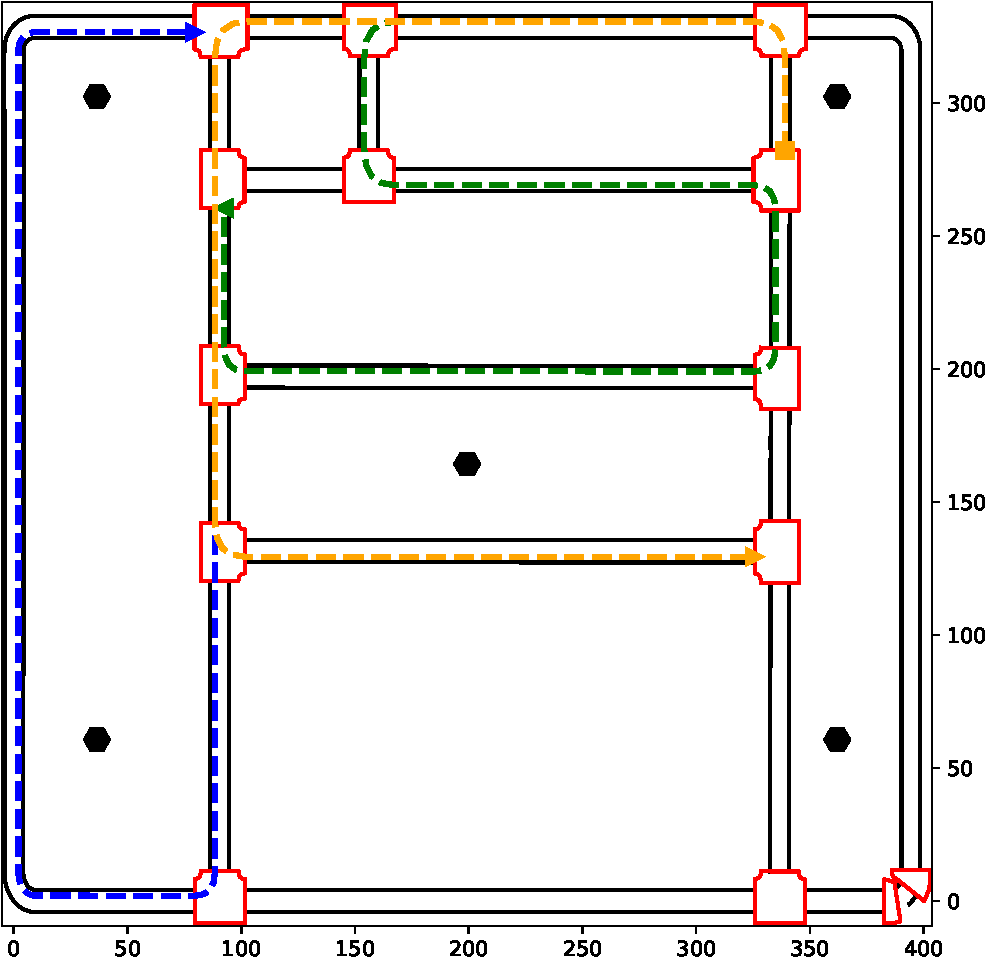
\includegraphics[width=1.0\textwidth]{chapter2/fig_traffic_map.pdf}
    \caption{The illustration of {\IAV} paths and BS locations on the road map.}
    \label{fig:traffic_map}
\end{figure*}

As for the performance benchmarks, we compare the proposed {\fwName} optimizer with the following ones.
\begin{itemize}
    \item \textbf{Equal-time Policy}:The one where all the {\IAVs} choose the maximum transmission power $P_{\max}$ and equal time allocation.
    % \item \textbf{Time-efficient Policy}: The one chooses the best channel conditioned one to transmit at each time slot, i.e., $\gamma_{m',t}=1$, $p_{m',t} = P_{\max}$, where $m' = \arg\min_{m} l_{m,t}$, $\forall t$.
    \item \textbf{Equal-rate Policy}: {The one chooses the best channel conditioned one to transmit at each time slot, i.e., $\gamma_{m',t}=1$, $p_{m',t} = P_{\max}$, where $m' = \arg\min_{m} l_{m,t}$, $\forall t$.}
    \item \textbf{One-shot Policy}: The one solves problem \textbf{P2$(k)$} once at the very start and then adopts the same policy for all the remaining time slots.
    % \item \textbf{Super-slot Only}: The one solves problem \textbf{P2$(k)$} at the start of every super slot, and adopts the same policy intermediately.
    \item \textbf{Exhaustive Policy}: The one optimizes problem \textbf{P2$(k)$} exhaustively at each time slot, i.e., $N=1$ in the {\fwName} optimizer;
    \item \textbf{Proposed Policy}: The one solves global and local optimization problems in the proposed {\fwName} optimizer alternatively with $N=5$.
\end{itemize}

\subsection{Performance Analysis}
\label{subsec:chapter2-performance}
First of all, we demonstrate how the transition of the {\IAV} locations is extracted as Markov transition chain in \figurename~\ref{fig:analyze_markov_chain}.
As shown in \figurename~\ref{fig:analyze_markov_chain}, the delta of transition changes periodically along the time slots, and the transition chain is stationary within around every 100 seconds.
\begin{figure*}
    \centering
    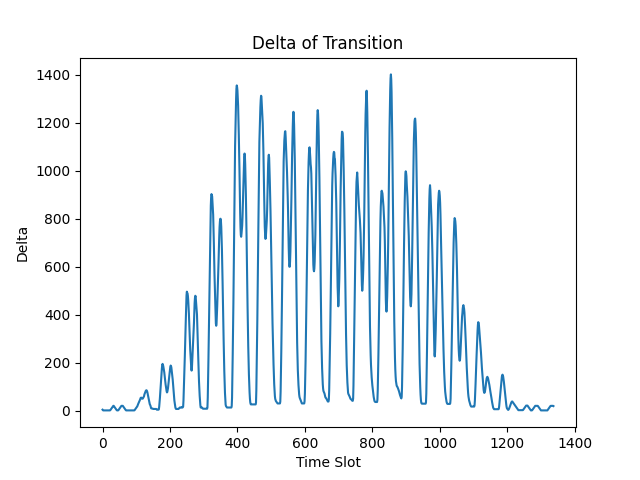
\includegraphics[width=1.0\textwidth]{chapter2/analyze_markov_chain.png}
    \caption{The stationary Markov transition chain of the {\IAV} locations.}
    \label{fig:analyze_markov_chain}
\end{figure*}

The total weighted cost of the proposed {\fwName} optimizer and the benchmarks are illustrated in the bar graph in \figurename~\ref{fig:analyze_total_cost}.
\begin{figure*}
    \centering
    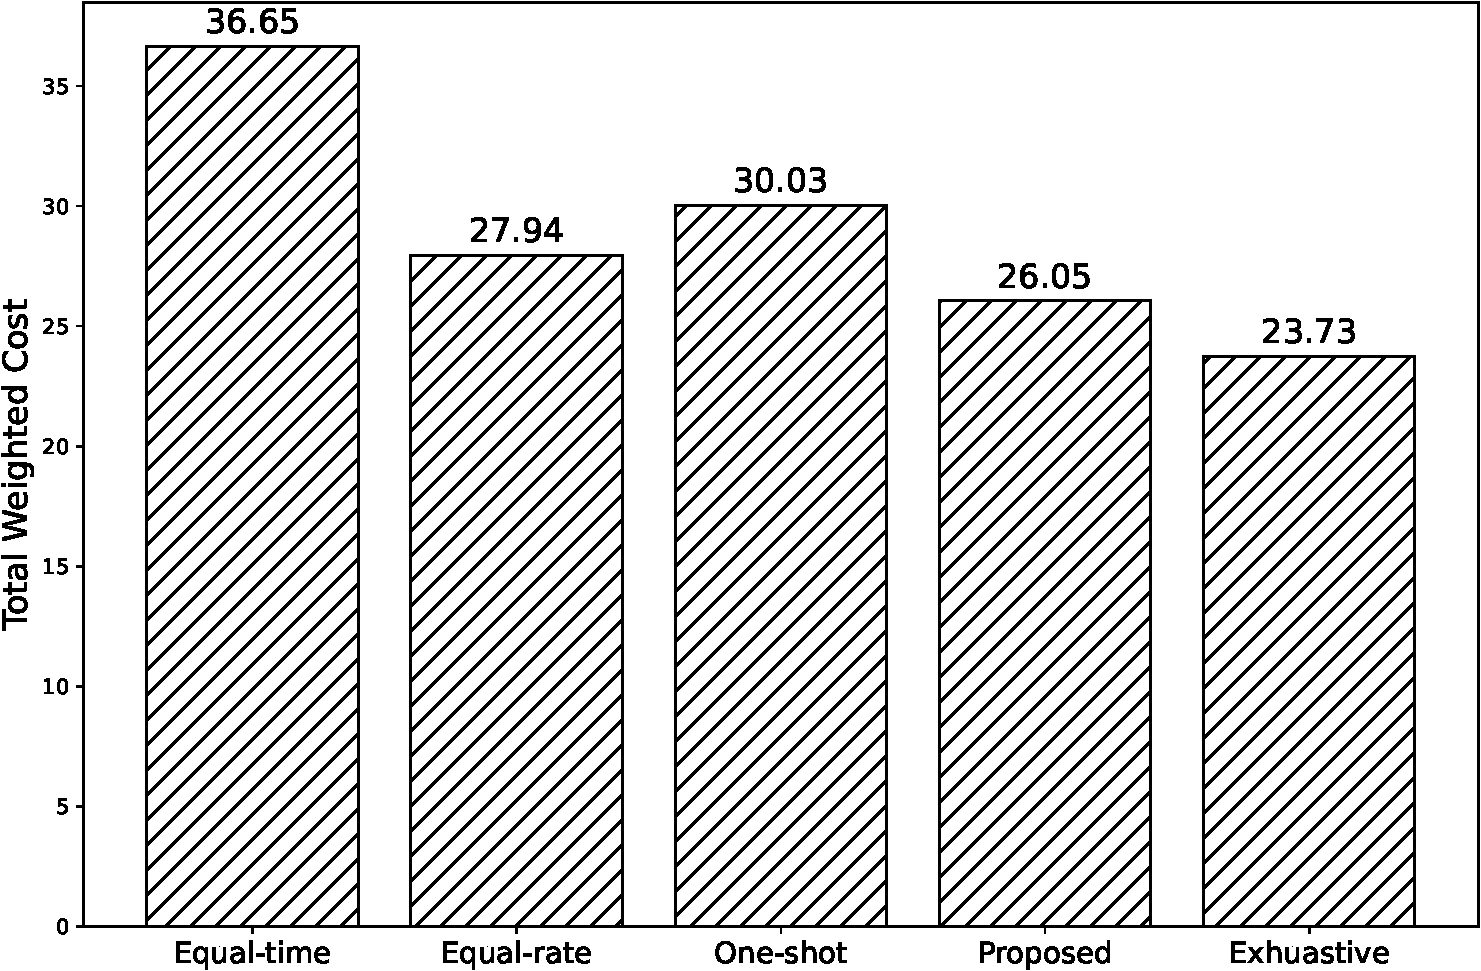
\includegraphics[width=1.0\textwidth]{chapter2/analyze_cost_bar.pdf}
    \caption{The total weighted cost of the proposed {\fwName} optimizer and the benchmarks.}
    \label{fig:analyze_total_cost}
\end{figure*}

\revise{
    It can be observed that the average overall cost of the {\fwName} optimizer is significantly better than the equal-time policy and the best-channel policy. The performance gain of the proposed {\fwName} optimizer over the decoupled policy is due to periodic optimization of problem \textbf{P2}.
}%
To further demonstrate the performance gap between the proposed {\fwName} optimizer and the benchmarks, we also plot the accumulated weighted cost versus time slots in \figurename~\ref{fig:analyze_accumulated_cost}.
\begin{figure*}
    \centering
    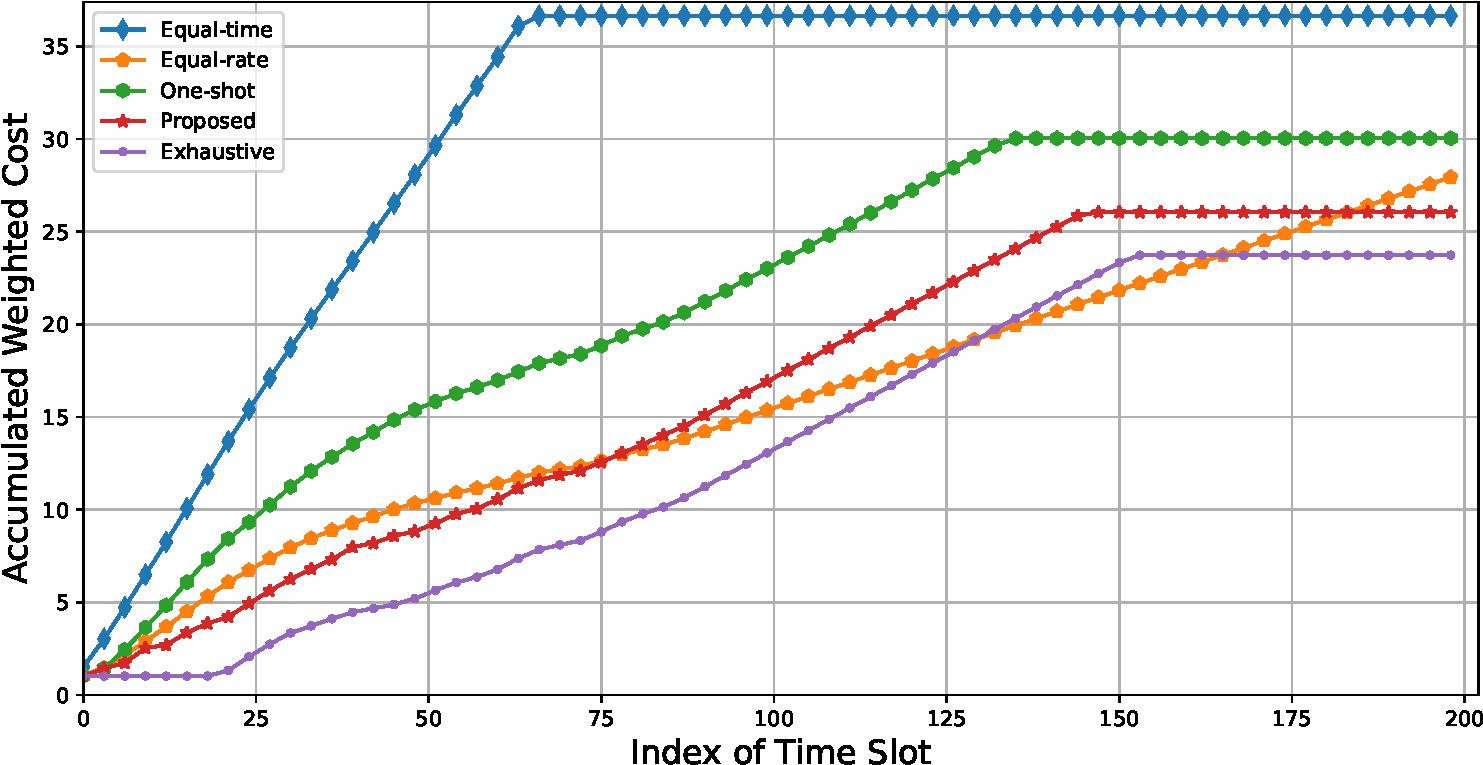
\includegraphics[width=1.0\textwidth]{chapter2/analyze_accumulated_cost.pdf}
    \caption{The accumulated weighted cost versus time slots.}
    \label{fig:analyze_accumulated_cost}
\end{figure*}

\subsection{Sensitivity Study}
\label{subsec:chapter2-sensitivity}
\noindent\textbf{Super slot Length $N$.}
The value function curve versus timeline w.r.t. various representative $N$ values.
\begin{figure*}
    \centering
    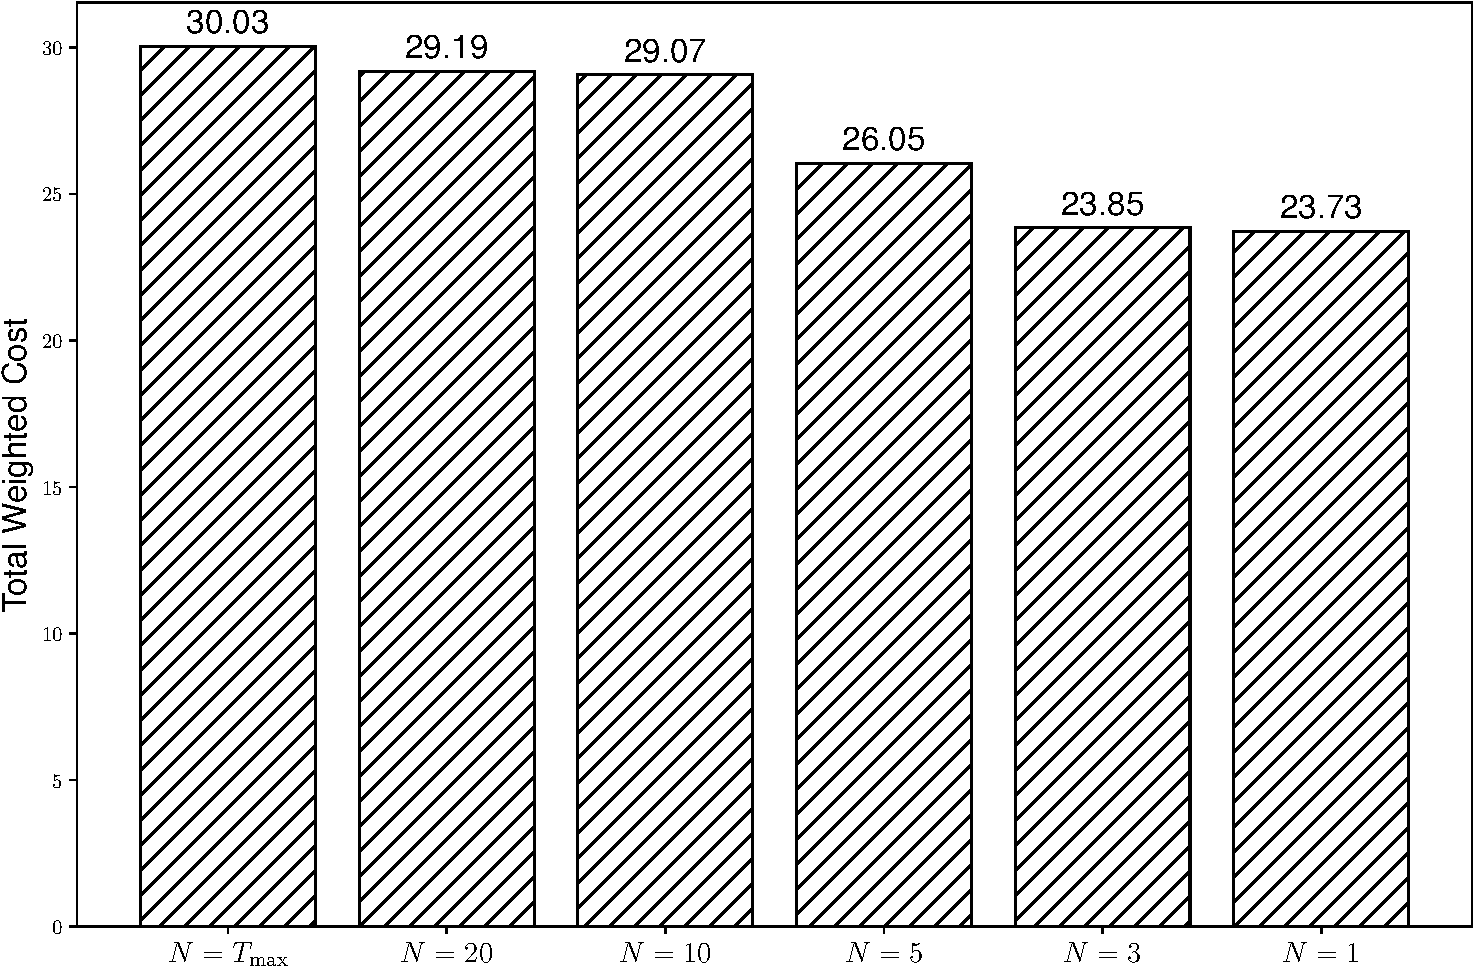
\includegraphics[width=1.0\textwidth]{chapter2/study_super_slot.pdf}
    \caption{The total weighted cost w.r.t different super slot length $N$.}
    \label{fig:study_super_slot}
\end{figure*}
The results show that smaller $N$ leads to better performance but higher computational complexity.


\noindent\textbf{Pareto Optimality}
The parameter $\omega$ tuning for balance of time-efficiency and energy-efficiency.
We sample different $\omega$ values and plot the Pareto curve.
\begin{figure*}
    \centering
    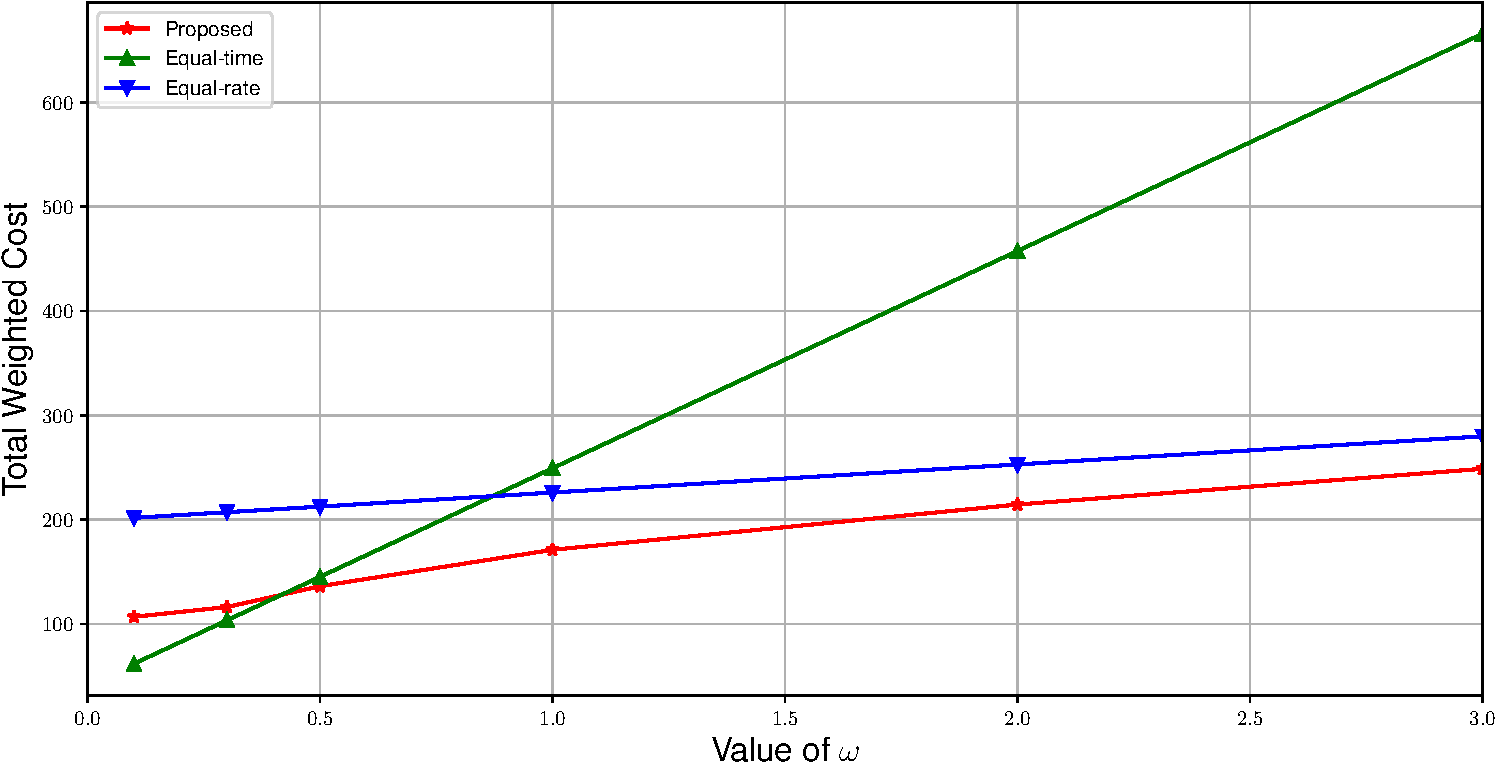
\includegraphics[width=1.0\textwidth]{chapter2/study_pareto_optimal.pdf}
    \caption{The total weighted cost under different weight $\omega$ and different algorithms.}
    \label{fig:study_pareto_optimal}
\end{figure*}
The results show that the proposed algorithm is Pareto optimal.

\noindent\textbf{Heterogeneity of Computation Capability.}
(1) all starts at same time, i.e., $T_{\text{comp},m}=0$, $\forall m\in\carSet$;
(2) only the driving-towards-BS ones starts earlier;
(3) only the driving-towards-BS ones starts later.
The results show that the proposed algorithm is robust to the heterogeneity of computation capability.


\section{Summary}
\label{sec:chapter2-conclusion}
We propose a data-driven framework called {\fwName} to study the communication scheduling problem for federated learning in vehicular networks.
The proposed {\fwName} framework is composed of two components: the high-fidelity trajectory dataset simulator and the {\fwName} optimizer.
In the {\fwName} trajectory simulator, we model the trajectory of each {\IAV} as a time-invariant Markov chain, and then formulate the communication scheduling problem as a finite-horizon MDP.
Since the optimal solution of the MDP suffers from the curse of dimensionality, we propose the {\fwName} optimizer to solve the problem in a low-complexity manner.
Specifically, every $N$ time slots are aggregated as \emph{super slot}.

The {\fwName} optimizer first determines the optimal time allocation policies for the remaining time slots at the beginning of each super slot.
Then, the {\fwName} optimizer determines the optimal power policies for each time slot for each {\IAV} independently.
The simulation results show that the proposed {\fwName} optimizer can achieve near-optimal performance with low complexity, and flexible trade-off between the performance and the computational complexity.
Furthermore, the hand-over among multiple base stations and the scheduling of multiple training epochs are not taken into consideration.

        % \revise{
\chapter{LeapFi: A Learning-based Application-oriented IEEE 802.11 System Channel Access Framework}
\label{ch3_after}

%=================================================================================================%
%=================================================================================================%

Reinforcement learning (RL) for radio resource management has attracted considerable attention, due to its promising ability to deal with unknown system statistics while significantly reducing the computational complexity compared to conventional model-based reinforcement learning approaches.
For example, it is prohibitively expensive to acquire co-channel interference caused by other traffics in unlicensed frequency bands, such as those used by the IEEE 802.11 system.
% it is also difficult to retrieve sufficient media access control (MAC) layer and physical (PHY) layer states from commercial Wi-Fi adapters.
Hence, the communication resource scheduling of a Wi-Fi network is challenging.
In this Chapter, we would like to leverage the state-of-the-art reinforcement learning techniques to facilitate the coordination of the Wi-Fi network transmission and to address the aforementioned practical constraints, so that the quality-of-service (QoS) of the heterogeneous applications is optimized.
% Moreover, the RL technique has also great potential to optimize a wireless system even without accurate or complete observation of the system state, which might happen in practical implementations.

There have been a significant amount of works optimizing the throughput~\cite{zhang2020drlthoughput,chu2018reinforcement,xu2020buffer}, delay~\cite{zhang2020delay} or age-of-information (AoI)~\cite{abd2020reinforcement,wu2022aoi,9839316} of wireless networks via the method of RL.
All these works assumed full knowledge of the system state in algorithm design, which could be applied on the systems where the global system state could be collected at a centralized controller. On the other hand, RL was also utilized to optimize the performance of wireless systems with distributive transmission scheduling, e.g., Wi-Fi systems. For instance, an adaptive channel contention mechanism was proposed for Wi-Fi systems in~\cite{kumar2021adaptive}, where a local RL agent is deployed at each user equipment (UE). The local agents adjust the minimum contention window (MCW) size according to the global statistics of successful channel contention such that the transmission fairness among the agents can be ensured.
% Enhancing Wi-Fi multiple access performance with federated deep reinforcement learning
Instead of global statistics, a distributive RL algorithm with the assistance of federated learning was proposed in~\cite{zhang2020enhancing} to adapt the channel contention according to the local channel state, such that the local throughput was optimized. Moreover, a deep multi-agent RL technique based on the QMIX algorithm~\cite{rashid2020monotonic} was proposed in~\cite{guo2022multi} to improve network throughput while maintaining user fairness. In this work, the channel contention decision was made according to the history of the last transmission duration. In order to resolve the collision issue of the distributive channel access, deep RL algorithms were proposed in~\cite{ali2018deep,ali2019q} to determine the timing of doubling the contention window based on the estimated collision probability.
% An Experience Driven Design for IEEE 802.11ac Rate Adaptation based on Reinforcement Learning
In addition to the adaptive channel contention, a double deep Q-network (DDQN)~\cite{van2016deep} based rate adaptation algorithm was proposed in~\cite{chen2021experience} to improve network throughput, where the agent learned the optimal transmission rate based on the modulation and coding scheme (MCS) and frame loss rate.

Most of the above literature assumed knowledge of the PHY-layer and MAC-layer system states. The RL techniques were exploited to tackle the unknown state transition probabilities or seek good scheduling policies from their enormous policy space. However, it might be challenging to obtain the knowledge of the PHY-layer and MAC-layer states in the controller design of a practical Wi-Fi network. Although there are some testbeds extracting the PHY-layer information from the adapter, e.g.,\cite{chen2021experience}, these methods would degrade the transmission performance due to hardware limitations and might not be generalized to most Wi-Fi adapters. Moreover, the absent knowledge on co-channel interference and the vendor-dependent implementation of Wi-Fi adapters would also raise challenge on the optimization of scheduling policies. 

In this Chapter, we would like to shed some light on the RL-based scheduling design for practical Wi-Fi systems suffering from unknown co-channel interference. Specifically, a learning-based framework for the application-layer QoS Optimization of Wi-Fi networks, namely {\algName}, is proposed for the scheduling of delay-sensitive communication tasks and throughput-hungry file delivery tasks. In {\algName}, a controller periodically collects the past scheduling parameters and average QoS observations of all the application-layer tasks, determines rate limitation and contention window size for all the transmitters, such that the total throughput of file delivery tasks is maximized and the latency requirements of delay-sensitive tasks are ensured. Because the relationship between the application-layer QoS and the transmission scheduling parameters is unknown, a novel Q-network design is proposed, which maps the historical scheduling parameters and QoS observations to the current scheduling action. Moreover, an imitation learning method is introduced to improve the training efficiency of the Q-network. It is shown by the experiments that the proposed framework can adapt to the variation of task number, interference traffic and link quality, and significantly outperforms the conventional EDCA mechanism.

\section{System Model}
In this section, the deployment scenario of the proposed {\algName} system is first elaborated, followed by the models of transmission and scheduling.

\subsection{Deployment Scenario}
\label{sec:Deployment Scenario}

The proposed {\algName} system is deployed in a Wi-Fi network (i.e., an extended service set, ESS) with multiple connected access points (APs) and user equipments (UEs) working on the same channel. Denote the number of the devices, including the APs and UEs, in the Wi-Fi network as $U$, the set of these devices as
\begin{equation}
    \devSet =\{u_{i}|{i}=\iterDeviceSet\},
\end{equation}
and the communication link from the $i$-th device to the $j$-th one as the {$(i,j)$}-th link ($\forall u_{i}, u_{j} \in \devSet$). The communication links can be from UE to AP, from AP to UE, or between UEs (i.e., Wi-Fi Direct~\cite{alliance2009wi}). We define $\linkset$ as the set of all communication links in the system and $\linkset_{i} $ as the set of communication links from the $u_{i}$-th device. As a remark, one UE could be with both the infrastructure and Wi-Fi Direct modes. Thus, it could simultaneously maintain the communication links to the AP and other UEs, where the transmission of the infrastructure and Wi-Fi Direct modes is separated in the time domain.

The data traffics raised by the applications of UEs in $\devSet$ are referred to as communication tasks in this Chapter. For example, the application projecting the screen of a mobile phone to a laptop via Wi-Fi Direct will raise a {\it delay-sensitive task}, e.g., Miracast~\cite{WiFiDisplay2011}, where an application-layer packet (i.e., video frame) is generated and delivered periodically (the typical period is $16$ ms). Large transmission latency of delay-sensitive tasks may lead to the issue of rebuffering, which degrades the experience of users. Moreover, file sharing between two devices will raise a {\it file delivery task}. For the elaboration convenience, we define $\thruTS$ and $\rttTS$ as the universal sets of file delivery tasks and delay-sensitive tasks on the $(i,j)$-th link, respectively. The joint scheduling of the file delivery and delay-sensitive tasks among the devices in $\devSet$ will be optimized in the proposed {\algName} system, where the tasks can be in the active or inactive state. A task is in the inactive state if there is no packet arrival or buffered file at the transmitter.

Because of the transmission latency constraint, the delay-sensitive tasks should be scheduled with higher priority than the file delivery ones. In order to facilitate the scheduling with heterogeneous priorities in the Wi-Fi network, all the transmitters access the channel via the mechanism of enhanced distributed channel access (EDCA) defined in IEEE 802.11e~\cite{802.11e}. Specifically, four access category (AC) queues, namely {voice (VI), video (VO), best effort (BE), and background (BK)}, are adopted at all the transmitters. The transmission priorities of the four AC queues are differentiated with different values of arbitration inter-frame spacing (AIFS) and contention window (CW) size. As in the practical systems, the file delivery tasks are scheduled with the BE priority, and the delay-sensitive tasks are scheduled with the VI priority. The latter has smaller AIFS and CW size, leading to a more significant successful probability in channel contention. As a remark, due to the distributive channel contention mechanism, it is infeasible to accurately control the order of packet transmission among the devices of a Wi-Fi network with commercial network interface cards (NICs). Instead, the packet transmission in the {\algName} system is scheduled in a stochastic manner by adapting the CW sizes of AC queues in each device.

There are some other Wi-Fi networks sharing the same channel in the coverage of the considered network. The traffic in these interfering networks would degrade the QoS of the considered network, e.g., larger packet delivery latency and lower throughput. Denote the set of devices in the interfering network as $\devSet_I$. The communications among the devices in $\devSet_I$, namely interfering traffic, cannot be scheduled by the {\algName} system. Instead, it is assumed that the interfering traffic varies slowly, such that the {\algName} system is able to deduce the interference level and adjust the transmission.

\subsection{Task Queuing Model}

The queuing dynamics of the file delivery and delay-sensitive tasks are elaborated in this section.
As illustrated in \figurename~\ref{fig:MAC}, the file delivery tasks are transmitted via the BE priority.
For each of them, all the information bits to be delivered are saved in an application-layer buffer, and a user datagram protocol (UDP) socket is established at the very beginning of transmission.
The data dispatch from the buffer to the UDP socket is controlled by a dispatcher.
The UDP socket encapsulates the received data from the dispatcher into UDP datagrams and forwards them to the driver of NIC for Wi-Fi transmission.
As a remark, the new datagrams that arrived at the NIC may not be transmitted immediately.
In fact, each NIC maintains four MAC-layer AC queues associated with the four transmission priorities, respectively.
The arrival datagrams are saved in the corresponding queues and transmitted following the vendor's protocol.
The queuing status of the NIC is usually not accessible in the application-layer.
Thus, it is infeasible for the proposed system to know when the NIC completely delivers a datagram; it is, therefore, infeasible for the proposed system to precisely control the transmission of a MAC protocol data unit (MPDU) or a UDP datagram. As a result, the scheduling of the proposed system is designed based on the average observable performance in the application layer.

Specifically, the transmission time is organized into a sequence of scheduling periods, each with a duration of $T_s$ seconds, which is sufficiently large to accommodate a number of MPDU transmissions. Due to the invisibility of NIC status, the QoS of a file delivery task is measured by its application-layer throughput in one scheduling period. Specifically, for the $m$-th file delivery task of the $(i,j)$-th link ($\forall \iterLink, \iterTaskThru, $), its QoS in the $t$-th scheduling period {$\eleThru(t)$} is defined as the number of information bits transferred from the task buffer to the associated UDP socket.
The dispatcher is designed to adaptively limit the throughput of the file delivery task such that delay-sensitive tasks could have a larger chance to access the channel. 
Hence, let $\eleThruLimit(t)$ be the throughput limitation of the $m$-th file delivery task of {$(i,j)$}-th link in the {$t$}-th scheduling slot, the dispatcher would make sure
\begin{align}
    \label{eq:throughput_limitation}
    \eleThru(t) \leq \eleThruLimit(t).
\end{align}

For each delay-sensitive task, a task queue and UDP socket are established at the very beginning. The application-layer packets arrive at the task queue periodically with a fixed average data rate. The first packet in the queue is forwarded to the UDP socket for Wi-Fi transmission as long as the socket is idle. Due to the lack of MAC-layer status, the measurement of the transmission latency of a packet could hardly be accurate. Hence, we use the round-trip time (RTT) as the QoS measurement of delay-sensitive communication tasks. Specifically, for each delay-sensitive task, an acknowledgment will be sent from the receiver to the transmitter when an application-layer packet is completely received. Hence, the transmitter can calculate the RTTs of all packet transmissions. For the {$m$}-th delay-sensitive task of the {$(i,j)$}-th link ($\forall \iterLink, \iterTaskRTT$), its QoS in the $t$-th scheduling period {$\eleRTT(t)$} is defined as the average RTT of the packets transmitted in this scheduling period.


\subsection{Scheduling Model}

In the existing literature on cross-layer scheduling, the transmission parameters in physical and MAC layers are usually optimized. Unlike these works, the proposed {\algName} system is {implemented} in the existing Wi-Fi networks, where all the devices are deployed with commercial Wi-Fi NICs. Most of the transmission parameters in the physical and MAC layers, including the user selection, power adaptation, beamforming, etc., are all encapsulated in the NICs and difficult to customize. Instead, the CW sizes of the four AC queues can be adjusted via the NIC driver. Denote the CW sizes of the VI and BE priorities of the ${i}$-th device as  $w_{i}^{\VI}$ and $w_{i}^{\BE}$ respectively, we shall focus on the joint scheduling of these channel contention parameters as well as the dispatchers' throughput limitation $\{\eleThruLimit(t)|\forall \iterLink,\iterTaskThru\}$ in each scheduling period.

The scheduling framework is illustrated in \figurename~\ref{fig:MAC}. Each transmitter collects the QoS observations of its tasks at the end of each scheduling period and delivers them to a centralized controller, which can be implemented in an AP or other device. Not all the tasks in the universal task sets are in the active state, the average RTTs and throughput of the inactive delay-sensitive and file delivery tasks are represented by a sufficiently large value and $0$, respectively. Hence, the aggregation of QoS observations received at the controller at the end of the $t$-th scheduling period can be represented as
\begin{align}
    \begin{split}
        \observation_{t} \define & \left\{\eleThru(t) |\forall \iterLink,\iterTaskThru \right\} \\ &\cup  \left\{\eleRTT(t)| \forall \iterLink,\iterTaskRTT \right\}.
    \end{split}
\end{align}
Due to the time-varying traffic of the interfering devices, the scheduling parameters, including the file throughput limitations and CW sizes, are adapted at the centralized controller in each scheduling period (say the $t$-th scheduling period) according to the system's scheduling parameters and QoS observations in the past $N$ scheduling periods. Specifically, the aggregation of scheduling parameters in the $t$-th scheduling period is represented as
\begin{align}
    \label{eq:action}
    \begin{split}
        \action_t \define & \left\{ \eleThruLimit(t) | \forall \iterLink,\iterTaskThru \right\} \\ &\cup  \left\{ w_{i}^{\VI}, w_{i}^{\BE} | i = \iterDeviceSet \right\}.
    \end{split}
\end{align}
Thus, at the very beginning of the $t$-th scheduling period, $\action_t$  ($\forall t$) is determined based on past scheduling parameters and QoS observations as follows:
\begin{equation}
    \{ (\observation_{t-N},\action_{t-N}),(\observation_{t-N+1},\action_{t-N+1}),\ldots,(\observation_{t-1},\action_{t-1})\}.\nonumber
\end{equation}

\begin{remark}[Performance Trade-Off]
    Heavy file delivery traffic will aggravate channel contention and degrade the RTT performance of the delay-sensitive communication tasks. Thus, throttling the throughput of file delivery traffic could improve the RTT performance of the latter tasks. Moreover, the RTT performance of different transmitters can also be traded off by adjusting their CW sizes. This motivates the optimization of both the throughput limitation and CW sizes in the proposed {\algName} system.
\end{remark}

\begin{figure}[!t]
    \centering
    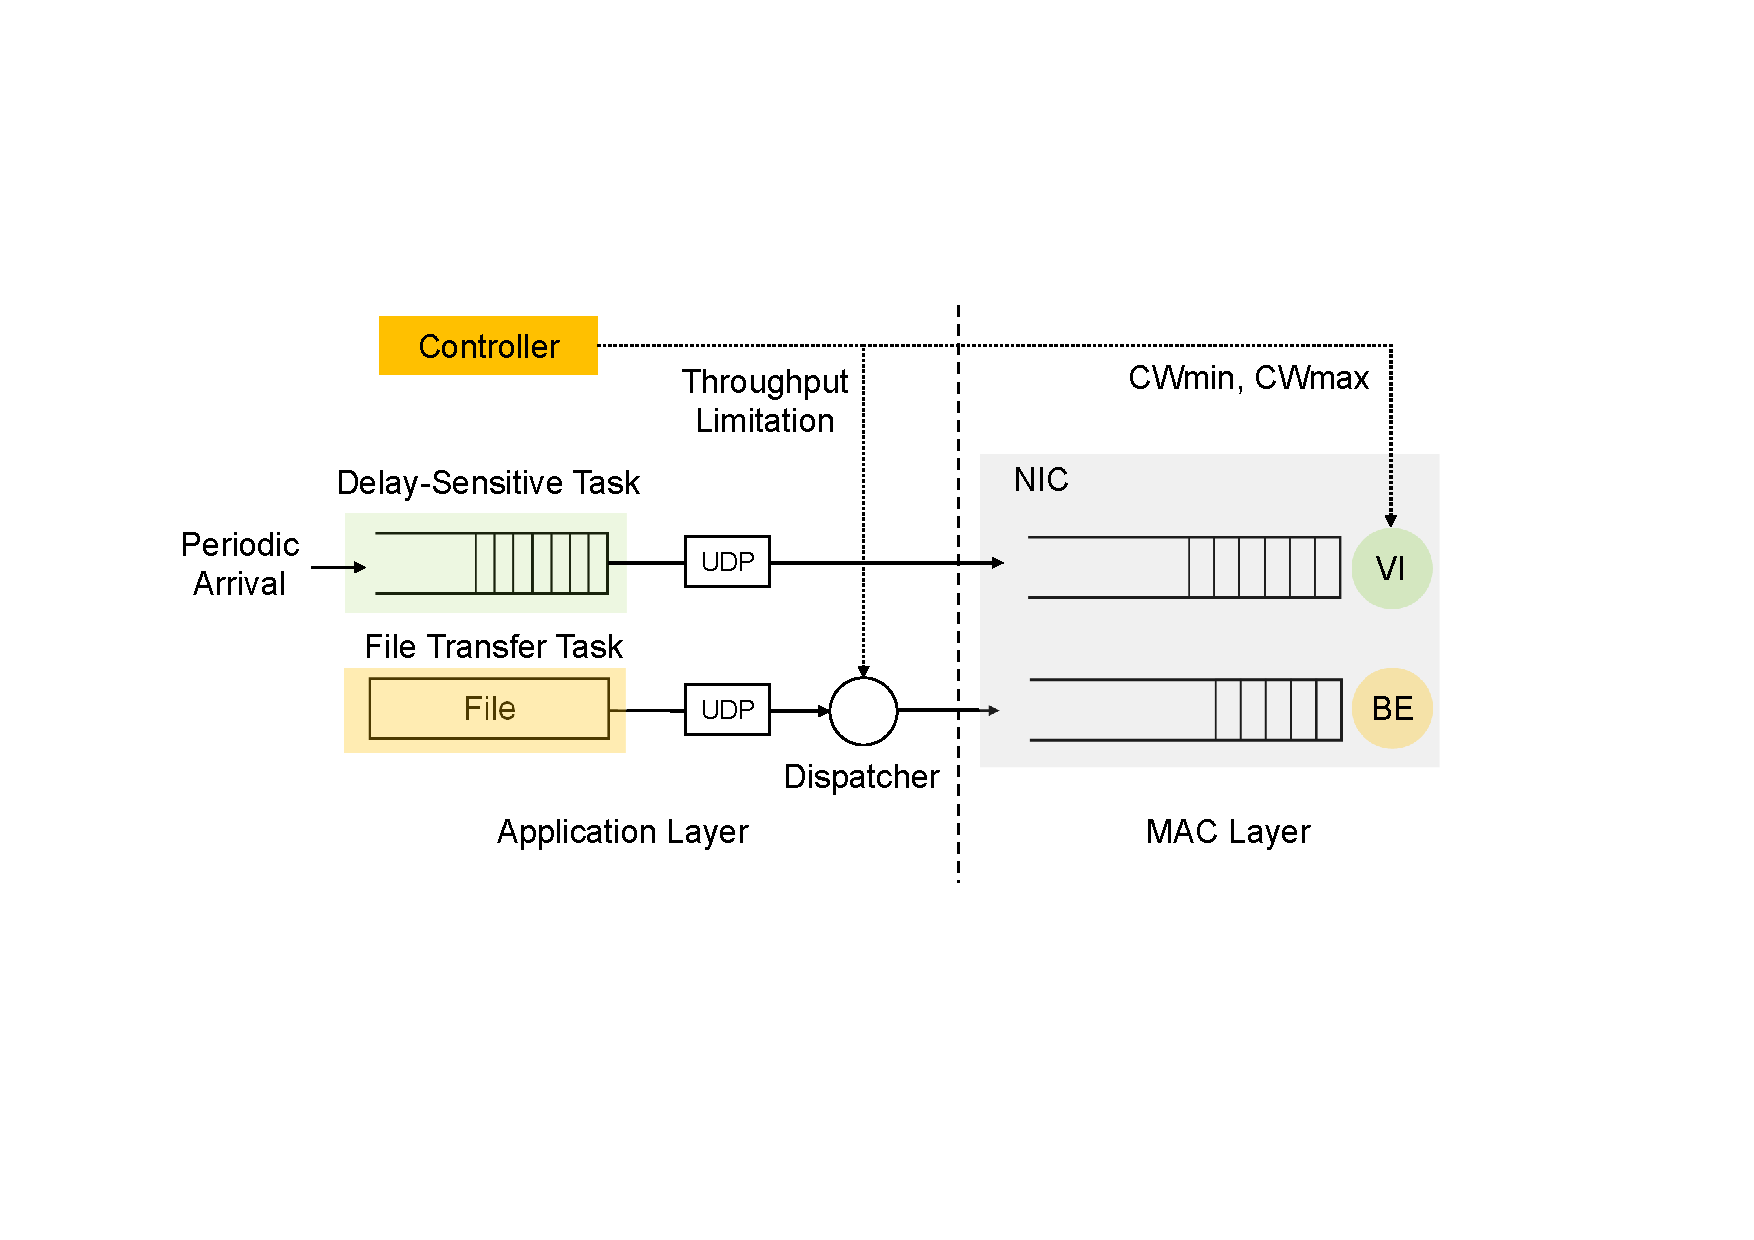
\includegraphics[width=\linewidth]{chapter3_after/MAC Queue Model 2.pdf}
    \caption{The Illustration of MAC Queue in Operating System.}
    \label{fig:MAC}
\end{figure}

\section{Problem Formulation}
\label{sec:Problem Formulation}
The proposed {\algName} system should successively make scheduling decisions for each scheduling period, which is formulated as a Markov decision process (MDP) in this section. Due to the co-channel interference, a complete description of the system state should include the traffic information of the devices in both $\devSet$ and $\devSet_I$, which is infeasible to obtain in the considered scenario. Instead, we treat the scheduling parameters and QoS observations of the past $N$ scheduling periods as the state of the current scheduling period, leading to a partially observable MDP (POMDP) with unknown state transition probabilities. Specifically, the system state, scheduling policy, and system cost are defined as follows.

\begin{definition}[System State] In the $t$-th scheduling period ($\forall t$), the system state is defined as the aggregation of the QoS observations and scheduling parameters of the past $N$ scheduling periods. Thus,
    \begin{equation}
        \state_t \define \left\{
        (\observation_{t-N},\action_{t-N}),\ldots,(\observation_{t-1},\action_{t-1})
        \right\}.
    \end{equation}
\end{definition}

\begin{definition}[Scheduling Action and Policy] Denote $\action_t$ defined in Equation (\ref{eq:action}) as the scheduling action in the $t$-th scheduling period,
\begin{equation}
    \action_t^i \define 
    \left\{ 
        b_{i,j}^m(t) | \forall j \in \linkset_i, \iterTaskThru 
    \right\} 
    \cup 
    \left\{ 
        w_{i}^{\VI}, w_{i}^{\BE} 
    \right\}.
\end{equation}
as the local scheduling action of the $i$-th device in the $t$-th scheduling period. The scheduling policy {$\Policy$} is a mapping from {state space} to {action space} as follows:
    \begin{equation}
        \Policy( \state_t ) = \action_t.
    \end{equation}
\end{definition}

Moreover, we define the system cost of the $t$-th scheduling period as
\begin{align}
    \label{eq:cost function}
    \begin{split}
        c_t(\state_t, \action_t)
        \define
         & \sum_{\iterLink} \sum_{\iterTaskRTT}
        \mathds{1}(\eleRTT(t) > \eleRTTLimit)                          \\
         & - \omega \sum_{\iterLink} \sum_{\iterTaskThru} \eleThru(t).
    \end{split}
\end{align}
where $\omega$ is a weight, $\eleRTTLimit$ is the maximum tolerable RTT of the $m$-th delay-sensitive task on the $(i,j)$-th link. The indicator function $\mathds{1}(\mathcal{E})$ is $1$ if the event $\mathcal{E}$, and $0$ otherwise.
Then, the average overall system cost is defined as the discounted summation of average system costs for all the scheduling periods, i.e.,
\begin{equation}
    \label{eq:average_cost}
    \averageCost(\Policy) = \lim_{T \rightarrow \infty} \mathbb{E}
    \bigg[
        \sum_{t = 1}^T \gamma^{t-1} c_t(\state_t, \Policy(\state_t))
        \bigg].
\end{equation}
For the elaboration convenience, it is assumed that the system has run for at least $N$ scheduling periods before the first scheduling period, such that there are sufficient QoS observations in the system state. As a result, the controller design of the {\algName} system can be formulated as
\begin{equation}
    \text{\bf Problem 1:} \ \min_{\Policy} \  \averageCost(\Policy).
\end{equation}
The Bellman's equations for the above MDP is given by
\begin{align}
    \label{eq:bellman}
    Q(\state_t, \action_t) = \mathbb{E}_{\state_{t+1}} \bigg[ c_t(\state_t, \action_t) + \gamma \min_{\action'} Q(\state_{t+1}, \action')  \bigg],
\end{align}
where $Q(\state_t, \action_t)$ is the Q-function with system state $\state_t$ and action $\action_t$. Moreover, the optimal scheduling action is given by

\begin{equation}
    \Policy^*(\state)  = \argmin\limits_{\action} Q(\state, \action).
\end{equation}

Given the past scheduling actions and QoS observations (i.e., the system state), it is still difficult to accurately predict the relation between the scheduling action and task QoS in the current scheduling period. This is because of the unknown interfering traffic. As a result, it is impossible to solve the above Bellman's equations without any trial on the network performance. In this work, we shall rely on the RL method to track the above unknown knowledge with the assistance of a preliminary observation dataset $\trainningDataSet$.

Specifically, the dataset $\trainningDataSet$ is collected from $M$ scheduling periods experiencing heterogeneous interfering traffic and link quality (e.g., the distances of links in $\linkset$ change due to mobility). Each of the scheduling periods (say the $\tau$-th one) is divided into two phases. In the first phase, a testing scheduling action $\classifyAction$ is applied, and corresponding QoS observation $\classifyObs_\tau$ is obtained; in the second phase, an arbitrary scheduling action $\trainAction_{\tau}$ according to certain criterion is applied, and another QoS observation $\trainObs_{\tau}$ is obtained. Hence,  the dataset $\trainningDataSet$  can be expressed as
\begin{equation}
    \trainningDataSet \define
    \left\{
    (\classifyObs_\tau, \classifyAction, \trainObs_{\tau}, \trainAction_{\tau})
    | \tau = \iterDataSet
    \right\}.
\end{equation}

\section{Q-Network for Online Scheduling}
\begin{figure}[!t]
   \centering
   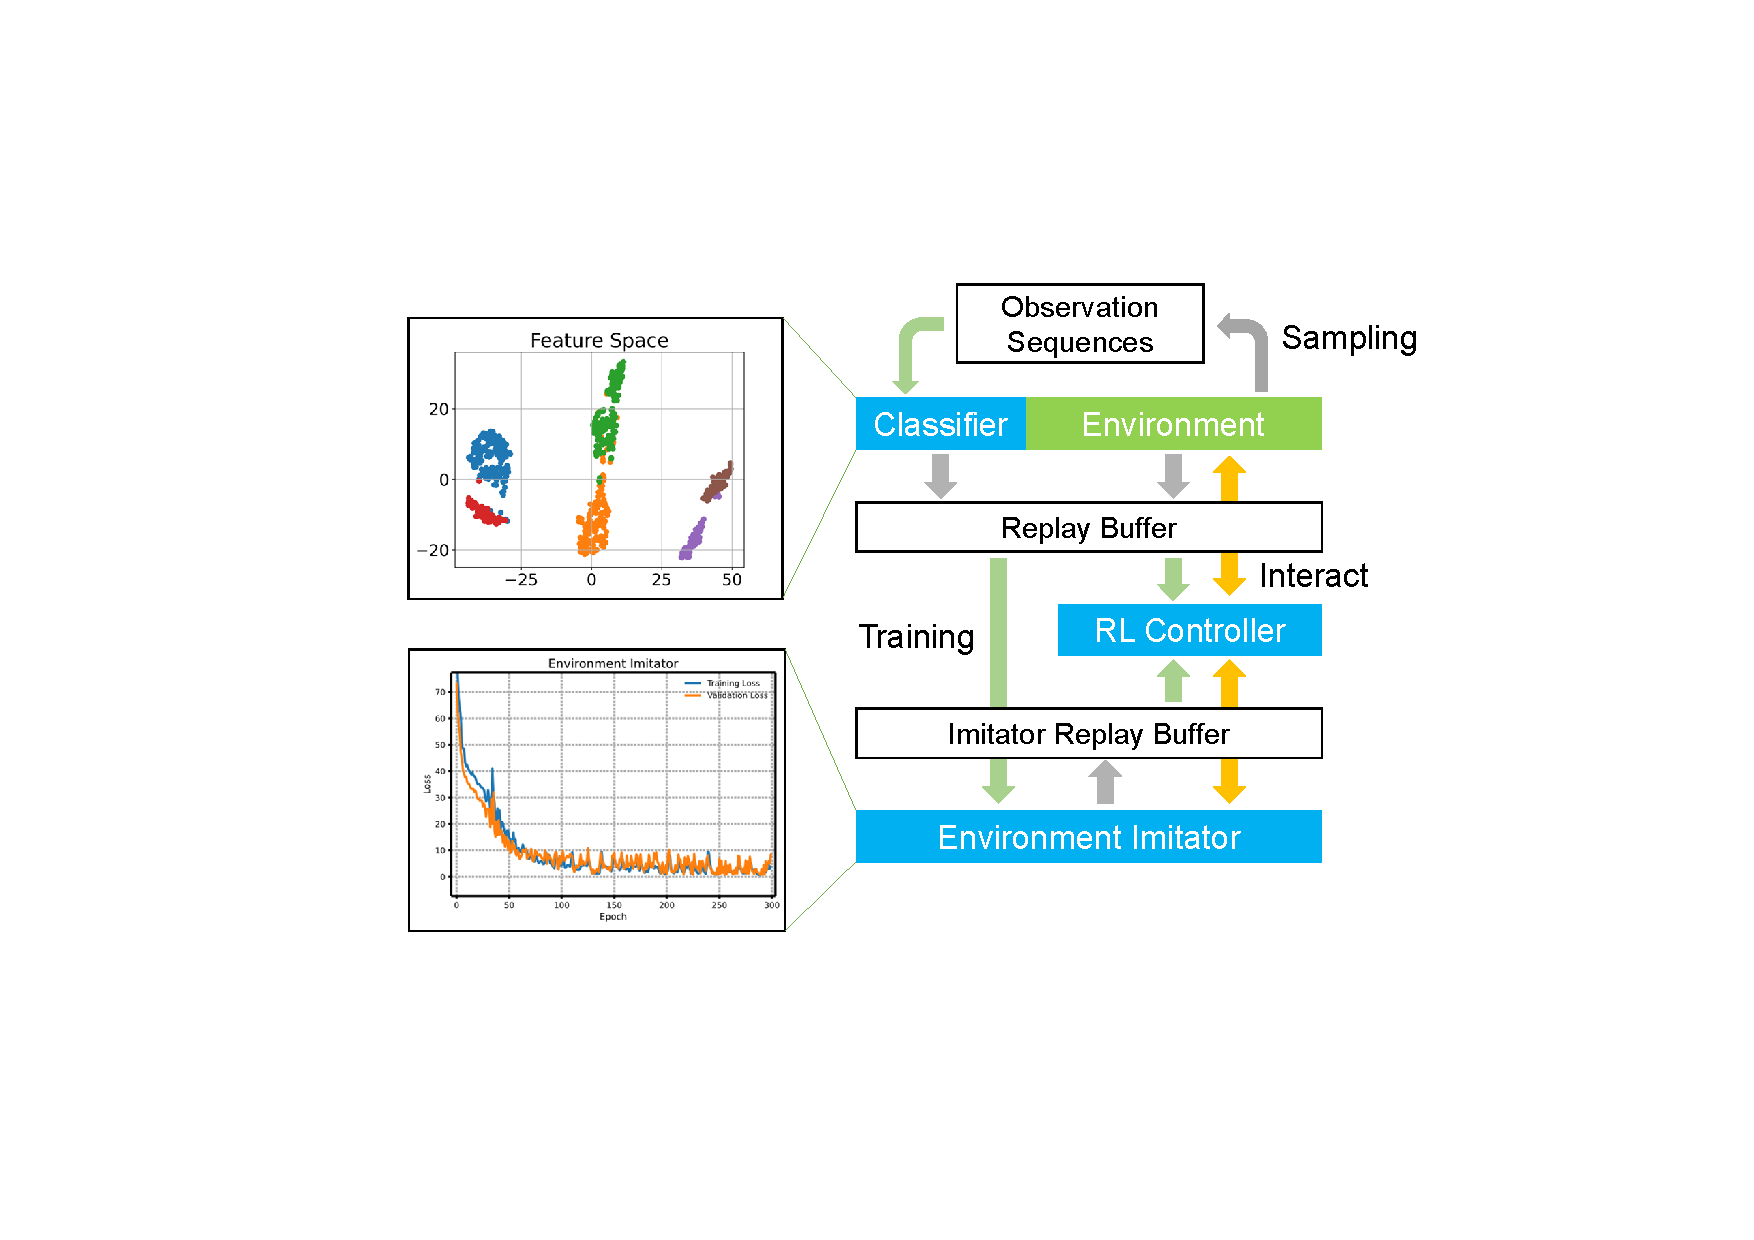
\includegraphics[width=0.9\linewidth]{chapter3_after/framework.pdf}
   \caption{The Illustration of {\algName} Online Scheduling.}
   \label{fig:framework}
\end{figure}

In this section, a novel Q-network design is proposed to approximate the Q-function defined in the previous section.
In order to accelerate the convergence of Q-network training and improve the scheduling performance, all the possible system performance of one scheduling period is divided into $K$ regions, and the inputs of the Q-network include not only the system state but also the \emph{performance region indices} of the past $N$ scheduling periods. 
Hence in this section, the offline performance region quantization based on the preliminary observation dataset $\trainningDataSet$ is introduced first, followed by the online testing of performance region index and the structure of the Q-network.

\subsection{Offline Performance Region Quantization}
\label{sec:performance Region Quantization}
The quantization of all the possible system performance is conduced based on the preliminary observation dataset $\trainningDataSet$ in an offline manner. Specifically, the QoS observations with the testing scheduling action $\classifyAction$ are extracted from the preliminary observation dataset $\trainningDataSet$ as follows:
\begin{equation}
   \classifyDataSet \define
   \left\{
   (\classifyObs_\tau, \classifyAction) | \tau = \iterDataSet
   \right\},
\end{equation}
The $K$-means classification method~\cite{macqueen1967some} is then adopted to classify the QoS observations in $\classifyDataSet$ into $K$ clusters, as illustrated in \figurename~\ref{fig:framework}. Denote the mean and variance of the observed throughputs (for the file delivery tasks) in $\classifyDataSet$ as $\avgThru$ and $\varThru^2$ respectively, the mean and variance of the RTTs (for the delay-sensitive tasks) as {$\avgRTT$ and $\varRTT^2$} respectively. Thus,
\begin{align}
   \avgThru & \define
   \frac{
      \sum_{\tau = 1}^M \sum_{\iterLink} \sum_{\iterTaskThru} \eleThruClassify(\tau)
   }{
      M \sum_{\iterLink} |\thruTS|
   },                    \\
   \avgRTT  & \define
   \frac{
      \sum_{\tau = 1}^M  \sum_{\iterLink} \sum_{\iterTaskRTT} \eleRTTClassify(\tau)
   }{
      M  \sum_{\iterLink} |\rttTS|
   },                    \\
   \varThru^2 & \define
      \frac{
         \sum_{\tau = 1}^M  \sum_{\iterLink} \sum_{\iterTaskThru}
         {\left(\eleThruClassify(\tau) - \avgThru\right)}^2
      }{
         M  \sum_{\iterLink} |\thruTS| - 1
      },                    \\
   \varRTT^2  & \define
      \frac{
         \sum_{\tau = 1}^M  \sum_{\iterLink} \sum_{\iterTaskRTT}
         {\left(\eleRTTClassify(\tau) - \avgRTT\right)}^2
      }{
         M  \sum_{\iterLink} |\rttTS| - 1
      },
\end{align}
where $\eleThruClassify$ and $\eleRTTClassify$ denote the average throughput and RTT of the $m$-th file-delivery task and delay-sensitive task on the $(i,j)$-th link in the dataset $\classifyDataSet$, respectively. Hence, the raw performance region quantization can be achieved by finding the $K$ cluster centers of the QoS observations in $\classifyDataSet$ as follows:
\begin{equation}
   \{\iterCCOpt\}  =
   \argmin
   \limits_{\iterCC} \
   \sum_{k=1}^K
   \sum_{\tau=1}^M
   \Vert \phi(\classifyObs_\tau) - \mu_k \Vert^2,
\end{equation}
where $\phi(\classifyObs_\tau)$ denotes the vectorization and normalization of the QoS observation $\classifyObs_\tau$. Specifically,
\begin{equation}
   \phi(\classifyObs_\tau) \define
   \left(
   \mathbf{r}_{\tau}^p, \mathbf{d}_{\tau}^p
   \right),
\end{equation}
where the row vector $\mathbf{r}_{\tau}^p$ vectorizes the normalized throughputs of all file delivery tasks
\begin{equation*}
   \left\{
      \frac{ \eleThruClassify(\tau) - \avgThru }{ \varThru }
      \bigg|
      \forall \iterLink, \iterTaskThru, \eleThruClassify(\tau) \in \classifyObs_\tau
   \right\},
\end{equation*}
and the row vector $\mathbf{d}_{\tau}^p$ vectorizes the normalized RTTs of all the delay-sensitive tasks
\begin{equation*}
   \left\{
      \frac{ \eleRTTClassify(\tau) - \avgRTT }{ \varRTT }
      \bigg| 
      \forall \iterLink, \iterTaskRTT, \eleRTTClassify(\tau) \in \classifyObs_\tau
   \right\}.
\end{equation*}

\subsection{Online Testing of Performance Region Index}

In the online transmission scheduling, a short testing slot can be reserved in each scheduling period, where the scheduling action $\classifyAction$ can be applied. Hence, the performance region index can be calculated according to
\begin{equation}
   \label{eq:raw performance region index}
   \rawPerRegion_t =
   \argmin\limits_{k} \
   \Vert \phi(\widehat{\observation}_t) - \mu_k^* \Vert^2,
\end{equation}
where $\widehat{\observation}_t$ is the QoS observation with the testing scheduling action $\classifyAction$ in the $t$-th scheduling period.

In the scenario where the performance region index varies slowly, the testing slot may not be applied in every scheduling period, and the performance region index of a scheduling period could follow the latest testing slot.

With the performance region quantization, we define the extended system state as follows.
\begin{definition}[Extended System State]
   Denote 
   $$
   \extendState_t \define 
   \left\{
      (\rawPerRegion_{t-N}, \observation_{t-N},\action_{t-N})
      ,\ldots,
      (\rawPerRegion_{t-1}, \observation_{t-1}, \action_{t-1})
   \right\}
   $$
   as the extended system state of the $t$-th scheduling period in the phase of online transmission scheduling, where $\rawPerRegion_{t-1}$ is the raw performance region index defined in Equation (\ref{eq:raw performance region index}).
\end{definition}

\subsection{Q-Network Structure}
\label{sec:Q-network}
\begin{figure}[!t]
   \centering
   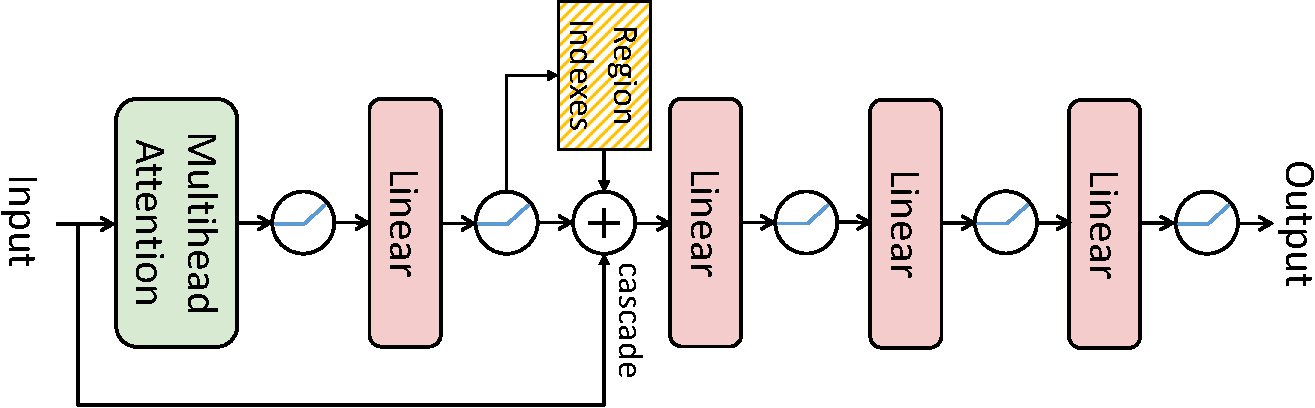
\includegraphics[width=\linewidth]{chapter3_after/Network Model 7.pdf}
   \caption{The Illustration of Novel Q-Network Design.}
   \label{fig:Network Design}
\end{figure}

The structure of the proposed Q-network is illustrated in \figurename~\ref{fig:Network Design}. Its input is the extended system state of the current scheduling period. The first part of the Q-network is a multi-head attention layer\cite{vaswani2017attention},  which is trained to refine the \emph{performance region indices} in the extended system state. The refined extended system state is then used as the input of the following three fully connected layers with $256$ nodes and ReLU activation function sequentially.

In order to address the issue of huge action space, we adopt the following linear approximation structure on the Q-function in the output of the Q-network:
\begin{equation}
   Q(\extendState, \action)
   \approx
   \sum_{{i} \in \devSet} Q^{i}(\extendState, \action^{i}),
\end{equation}
where $Q^{i}(\extendState, \action^{i})$ is referred to as the local Q-function of the ${i}$-th device. Hence, the Q-network output consists of $U$ action clusters for $U$ devices, respectively. Each action cluster provides the values of the corresponding local Q-function for all possible local actions. As a result, the optimized local action of the $i$-th device ($\forall i$) can be obtained by minimizing the local Q-function, i.e.,
\begin{equation}
   \action^{i}_t = \argmin\limits_{\action^{i}} Q^{i}(\extendState_t, \action^{i}).
\end{equation}

\section{Hybrid Q-Learning}
\label{sec:Hybrid Q-Learning}
\begin{figure*}[!t]
   \normalsize
   \begin{align}
      \label{eq: imitator loss}
      \imitatorLoss(\inetParam_k) = \frac{1}{|\trainObs_{\tau}|} \Bigg[
         \alpha
         &\sum_{\iterLink} \sum_{\iterTaskThru}
         {\left(\elePreThru(\action; \inetParam_k) - \eleThru(\tau)\right)}^2
         +
         \nonumber\\
         &\sum_{\iterLink} \sum_{\iterTaskRTTAlt}
         {\left(
            \elePreRTT(\action; \inetParam_k)
            -
            \min \left\{
            \eleRTTAlt(\tau), \beta \mathrm{D}^{n}_{i,j}
            \right\}
         \right)}^2
         \Bigg].
   \end{align}
   \begin{align}
      \label{eq:loss}
      \ctlLoss(\qnetParam_t) = \mathbb{E} \left[
         {\left( c_t\left(\state_t,\action_t\right)
         + \gamma \sum_{{i} \in \devSet}
         \min_{\action^{i'}}
         Q^{i} \left( \extendState_{t+1}, \action^{i'}; \qtnetParam_t \right)
         - \sum_{{i} \in \devSet}
         Q^{i} \left(
         \extendState_t, \action^{i}_t; \qnetParam_t
         \right)
         \right)}^2
         \right].
   \end{align}
   \hrulefill{}
\end{figure*}

The Q-network proposed in the previous section should be trained via the following two phases: the first offline training phase based on the dataset $\trainningDataSet$ and the second online tuning phase during the transmission scheduling. Both phases are elaborated in the following.


\subsection{Offline Q-learning}  

To facilitate the offline training, the performance indexes are calculated for all the scheduling periods in $\trainningDataSet$ according to Equation (\ref{eq:raw performance region index}). Denote the performance index of the $\tau$-th scheduling period in $\trainningDataSet$ as $\rawPerRegion_\tau^s$, the preliminary dataset $\trainningDataSet$ can be rewritten as
\begin{equation}
   \trainningDataSetwithRawPerInd  \define
   \left\{
   (\rawPerRegion_\tau^s, \observation_{\tau}^s, \action^s_{\tau})
   |
   \tau = \iterDataSet
   \right\}
\end{equation}
for notation convenience. Moreover, dataset $\trainningDataSetwithRawPerInd$ can be further divided into $K$ subsets as
\begin{equation}
   \trainningDataSetwithRawPerInd_k
   \define \left\{
   (k, \observation_{\tau}^s, \action^s_{\tau})
   |
   \forall \rawPerRegion_\tau^s = k
   \right\}
   \subset
   \trainningDataSetwithRawPerInd, k = \iterCCIdx.
\end{equation}

Notice that the subsets $\trainningDataSetwithRawPerInd_k$ ($k=\iterCCIdx$) may not be sufficiently large for the training of the Q-network in all the performance regions, the imitation learning method is introduced. Specifically, we first train $K$ DNN networks (namely imitators), each of which consists of $10$ fully connected layers and $256$ nodes per layer, to imitate the relation between the scheduling actions and QoS observations in the $K$ subsets, respectively. Denote the imitators as $$f(\action; \inetParam_k), k=\iterCCIdx,$$ where $\action$ is the input action, and $\inetParam_k$ represents network parameters of $k$-th performance region. The output of imitator $f(\action; \inetParam_k)$ is trained to approximate the QoS observation of the system in the $k$-th performance region with input action $\action$. Then, the Q-network can be trained via the $K$ imitators respectively.


{\bf Imitator training:} Let $\elePreThru(\action; \inetParam_k)$ and $\elePreRTT(\action; \inetParam_k)$ be the throughput and RTT of the ${m}$-th file delivery task and ${n}$-th delay-sensitive task of the $(i,j)$-th link in the output of the $k$-th imitator with input action $\action$.
The loss function of the $k$-th imitator for the training sample $(k,\trainObs_\tau, \trainAction_\tau) \in \trainningDataSetwithRawPerInd_k$, denoted as $\imitatorLoss$, is defined as Equation (\ref{eq: imitator loss}), where $r^{(m)}_{i,j}(\tau),d^{(n)}_{i,j}(\tau) \in \observation_{\tau}^s$,  $\alpha$ and $\beta$ are both weights, and the minimization is to limit the range of RTTs.

%% the imitator memory buffer
{\bf Q-network training:}  Based on the imitators, the Q-network can be trained in each performance region respectively according to the Q-learning method~\cite{mnih2015human}, where the outputs of the $k$-th imitator are treated as the QoS observations in the $k$-th performance region ($\forall k$). The loss function of the Q-learning, $\ctlLoss(\qnetParam_t)$, is defined in Equation (\ref{eq:loss}), where $Q(\cdot, \cdot; \qnetParam_{t})$ represents the Q-network updated in $t$-th scheduling period, and $\qtnetParam_t$ denotes the parameter of target network following~\cite{mnih2015human} to stabilize the training loss $\ctlLoss(\qnetParam_t)$. 

In order to efficiently explore the action space, an upper confidence bound (UCB) based exploration policy is introduced for the offline training of Q-network. Taking the Q-learning with the $k$-th imitator as the example, we first define the UCB of the action $\action^{i}$ of ${i}$-th device in the $t$-th offline scheduling period stage as
\begin{equation}
   \label{eq:UCB}
   UCB_{t}(k, \action^{i}) =
   Q_{t}^{i}(\extendState_t, \action^{i}; \qnetParam_{t})
   +
   \sqrt{\frac{4\eta\ln t}{T_{t}( k , \action^{i})}},
\end{equation}
where $T_t(k,\action^{i})$ counts the number of times the action $\action^{i}$ is taken up to the $t$-th scheduling period. The hyper-parameter $\eta$ is used to balance the exploration and exploitation.
As a result, in the $t$-th scheduling period of the offline training phase, the scheduling action is determined as follows:
\begin{equation}
   \label{eq:UCB epolicy}
   \action_t^{i} = \begin{cases}
      \argmin UCB_{t}(k, \action^{i}) & \text{with probability } 1 - \epsilon_t, \\
      \action^{i} \sim \uniformDis(\actionSpace^{i}) & \text{with probability } \epsilon_t,
   \end{cases}
\end{equation}
where $\uniformDis(\actionSpace^{i})$ is the uniform distribution over action space $\actionSpace^{i}$ of ${i}$-th device and exploration rate $\epsilon_t$ should satisfy the limit condition $\lim_{t \to \infty} \epsilon_t = 0$.

\subsection{Online Q-learning} 
The Q-network after the offline training is adopted in online scheduling. Meanwhile, the online training with the same loss function as in Equation (\ref{eq:loss}) could be applied to further improve the performance of the proposed {\algName} system. Specifically, in the $t$-th scheduling period of online training, the scheduling action of the ${i}$-th device, denoted as $\action_t^i$, is determined by the $\epsilon$-greedy policy as follows:
\begin{equation}
   \label{eq:online epolicy}
   \action_t^{i} = \begin{cases}
      \argmin Q^{i}(\extendState_t, \action^{i}; \netParam_{t}) & \text{with probability } 1 - \epsilon_t, \\
      \action^{i} \sim \uniformDis(\actionSpace^{i})            & \text{with probability } \epsilon_t,
   \end{cases}
\end{equation}
where $\epsilon_t$ and $\uniformDis(\actionSpace^{i})$ are defined in Equation (\ref{eq:UCB epolicy}).

\section{Experiments}
\label{sec:chapter3_after-testbed}

\begin{figure}[!t]
    \centering
    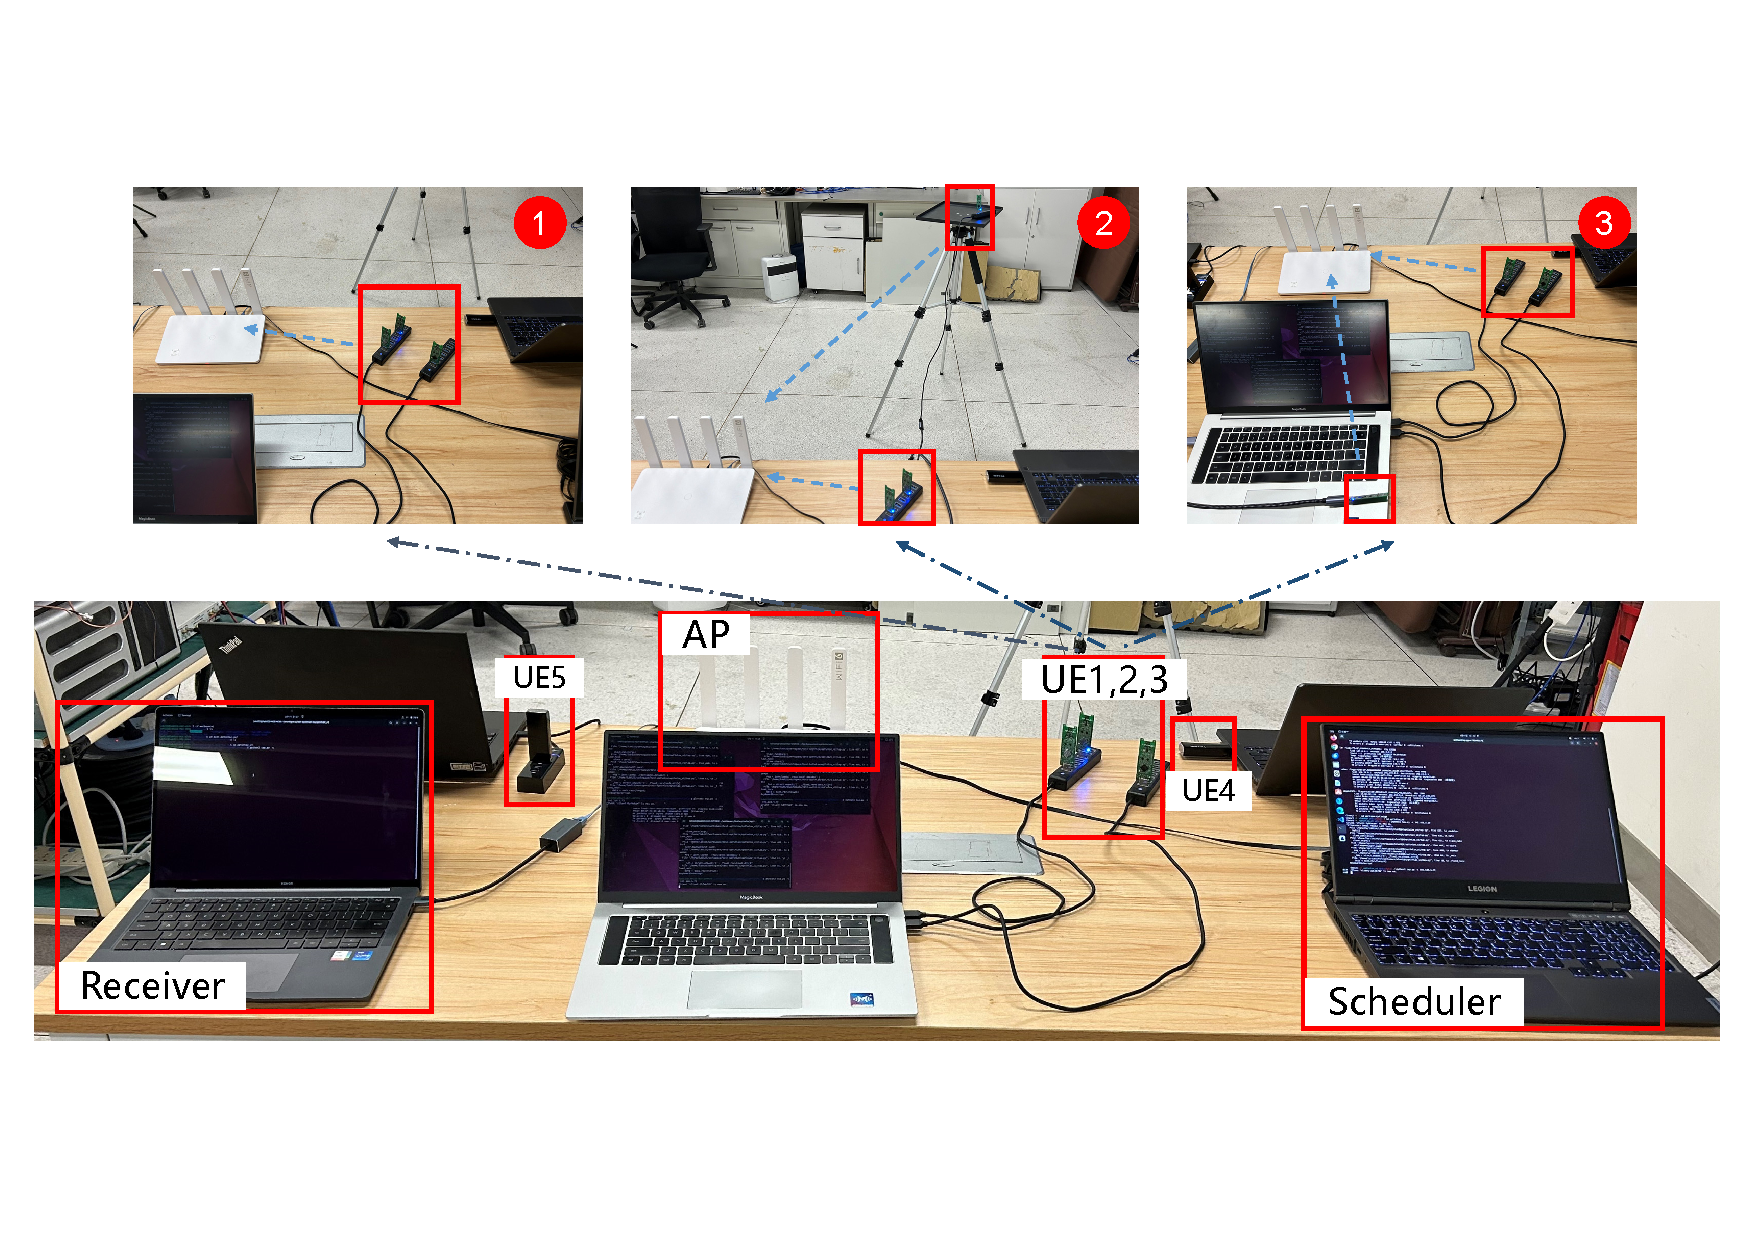
\includegraphics[width=1\linewidth]{chapter3_after/testbed-4.pdf}
    \caption{The testbed for experiments: below, the transmission scenario; above, $3$ evaluation examples.}
    \label{fig:Testbed Setup}
\end{figure}

As illustrated in \figurename~\ref{fig:Testbed Setup}, the proposed {\algName} framework is implemented in a Wi-Fi network with one HONOR XD30 AP and $3$ UEs each equipped with a TP-Link TL-WDN62000 USB Wi-Fi adapter in the experiment. 
Denote the AP as $u_0$ and the three UEs as $u_1, u_2, u_3$, respectively. 
% Reference: https://www.tp-link.com.cn/product_364.html?v=specification
The network is working on the 5GHz Wi-Fi band following the IEEE802.11ac specification.
The real-time controller is implemented in a laptop with Intel Core i7-8750H CPU and Ubuntu 20.04 operating system. % chktex 8
An Ethernet connection with a maximum data rate of $1$ Gbps is employed to facilitate communication between the controller and the AP.\@ 
Moreover, we rely on the Linux module \textit{wlspos\_hack}~\cite{lasso-sustech_wlsops-hack_2023} to adapt the CW sizes of TL-WDN62000 adapters in real-time from user space. 
Hence, the controller can collect the QoS observations from the three UEs and notify the scheduling actions via Wi-Fi, such that the UEs' transmission scheduling can be adjusted accordingly.

Both file delivery tasks and delay-sensitive tasks are tested in the experiment. The former tasks with a sufficient backlog are transmitted with the BE priority. The latter tasks, consisting of two types, are delivered with the VI priority. The data rates of type I and II delay-sensitive tasks are $\lambda_1 = 50$Mbps and $\lambda_2 = 25$Mbps, respectively. The packet arrival intervals of the two types are both  $16$ ms. Moreover, the maximum tolerable RTTs are $16$ms and $28$ms, respectively. The universal set of communication tasks tested in the experiment includes:
\begin{itemize}
    \item A delay-sensitive task with arrival data rate $\lambda_1$ (Task 1) and a file delivery task (Task 2) on the $(u_1,u_0)$-th link;
    \item A delay-sensitive task with arrival data rate $\lambda_2$ (Task 3) on the $(u_2,u_0)$-th link;
    \item A delay-sensitive task with arrival data rate $\lambda_2$ (Task 4) on the $(u_3,u_0)$-th link.
\end{itemize}
The quality of the $(u_1,u_0)$-th, $(u_2,u_0)$-th and $(u_3,u_0)$-th links depends on their distances and the propagation environment, which could be changed in the experiment. 

In the experiment, the duration of scheduling period is 1 seconds, the CW size takes values from $\{2^{i} \mid i = 0,1,2,\dots,10\}$ and throughput limitation takes values from $\{ \frac{i}{20} r_{i,j}^{({m},\max)} \mid i =0,1,2,\dots,20\}$, where $r_{i,j}^{({m},\max)}$ = 600 Mbps. Moreover, in addition to the background interference, the interfering traffic between two interfering UEs, denoted as $u_4$ and $u_5$, 
is also generated with random data rate and BE priority in the same channel. 

The preliminary observation dataset $\trainningDataSet$ are collected from the following three different traffic patterns: (1) Tasks 1 and 2 are activated; (2) Tasks 1, 2, and 3 are activated; and (3) Tasks 1, 2, 3 and 4 are activated. In all the traffic patterns, the communication distances of the links are altered to exploit the diversity of link rates. In the collection of  $\trainningDataSet$, the testing scheduling action $\action^p$ is first applied in the first half of the scheduling period, where the CW size and throughput limitation are $7$ and $300$ Mbps respectively. Then, a randomized action is applied in the second half. QoS observations of both actions are collected in each scheduling period. 

To demonstrate the performance gain, the proposed framework is compared with two baselines. The first baseline relies on the conventional 802.11 EDCA protocol. The second baseline only adapts the throughput limitation of file delivery tasks via the proposed framework, the control of the CW size follows the conventional 802.11 EDCA protocol.

\subsection{Imitator and Q-Network Training}

\begin{figure}[!t]
    \centering
    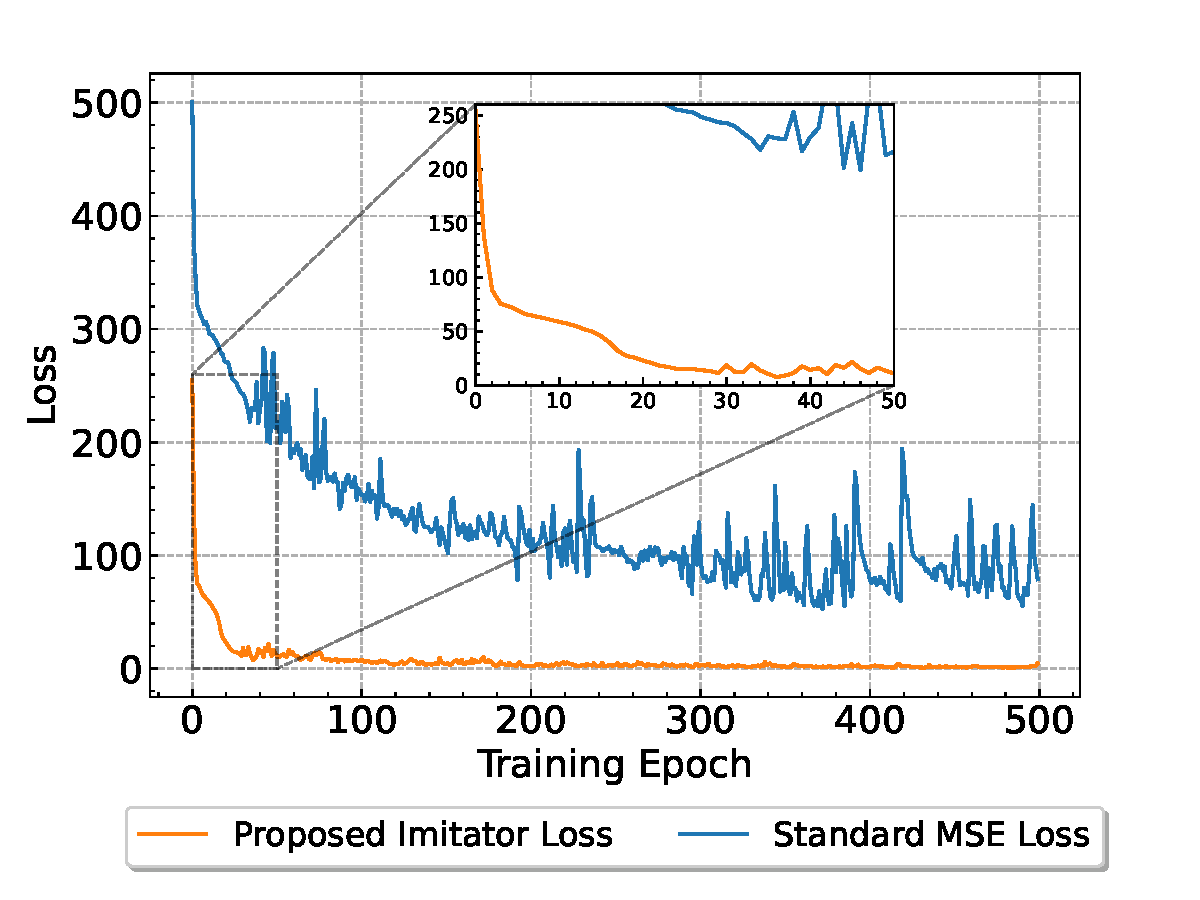
\includegraphics[width=\linewidth]{chapter3_after/loss compare-7.pdf}
    \caption{Comparing imitator training loss: proposed imitator loss function (\ref{eq: imitator loss}) versus standard MSE loss.}
    \label{fig:imitator training loss} % chktex 24
\end{figure}
\begin{figure}[!t]
    \centering
    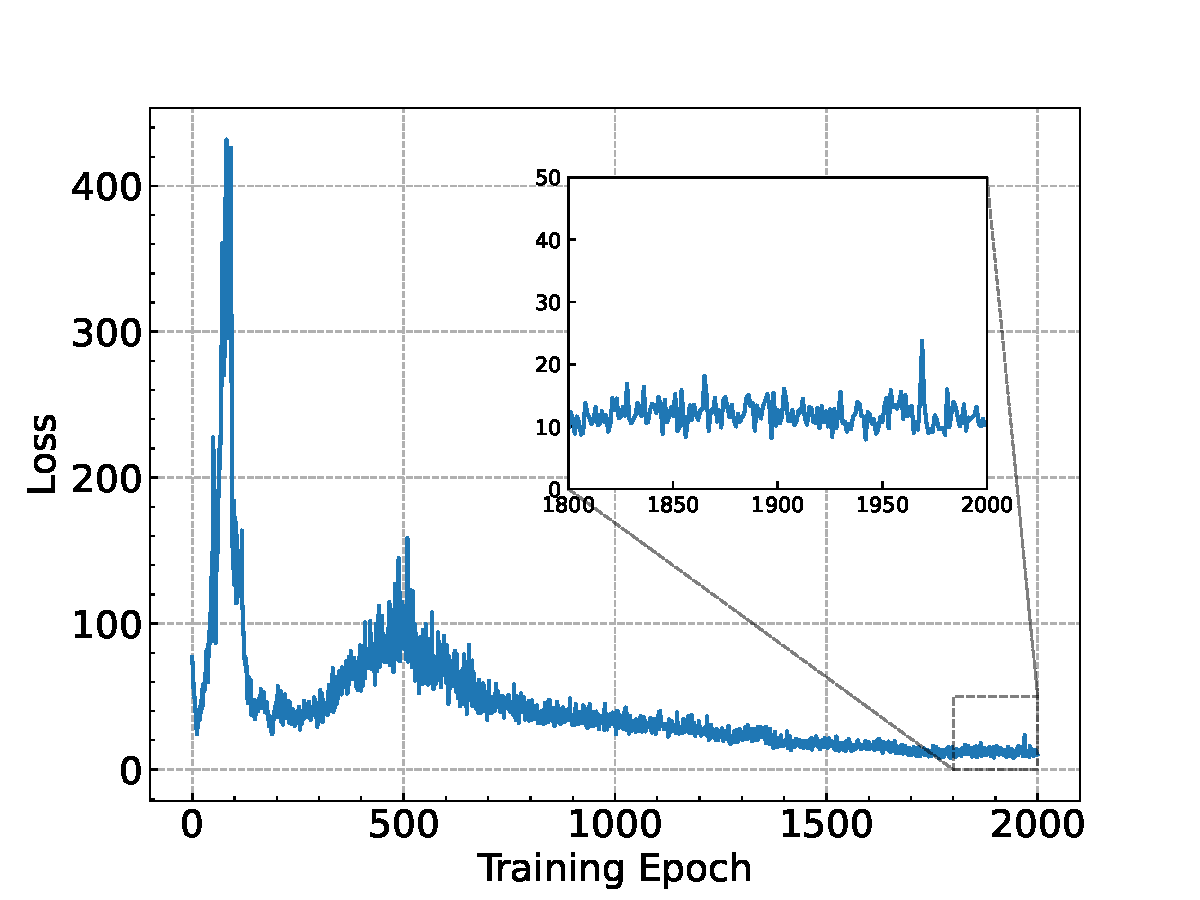
\includegraphics[width=\linewidth]{chapter3_after/rl_loss_2.pdf}
    \caption{The scheduler training loss following Equation (\ref{eq:loss}).}
    \label{fig:scheduler training loss} % chktex 24
\end{figure}
\begin{figure*}[!t]
    \centering
    \begin{minipage}[b]{0.32\linewidth}
        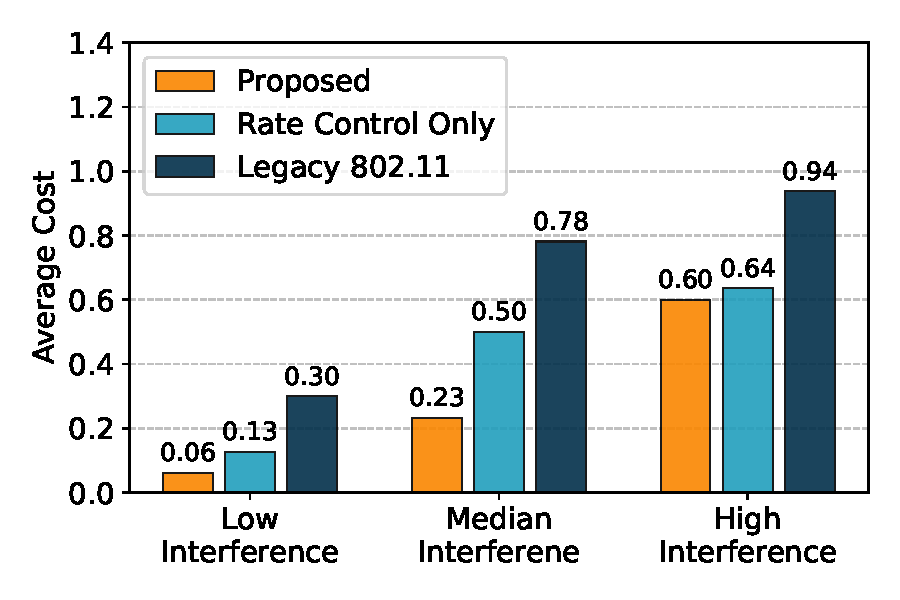
\includegraphics[width=\linewidth]{chapter3_after/Scenario 1-Average Cost 5.pdf}
        \caption*{(a) Scenario 1}
    \end{minipage}
    \begin{minipage}[b]{0.32\linewidth}
        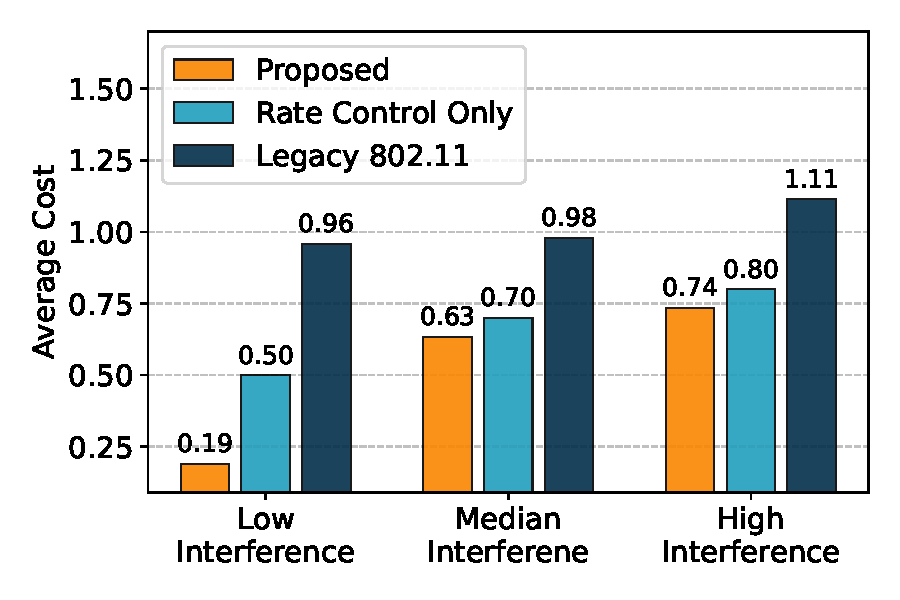
\includegraphics[width=\linewidth]{chapter3_after/Scenario 2-Average Cost 5.pdf}
        \caption*{(b) Scenario 2}
    \end{minipage}
    \begin{minipage}[b]{0.32\linewidth}
        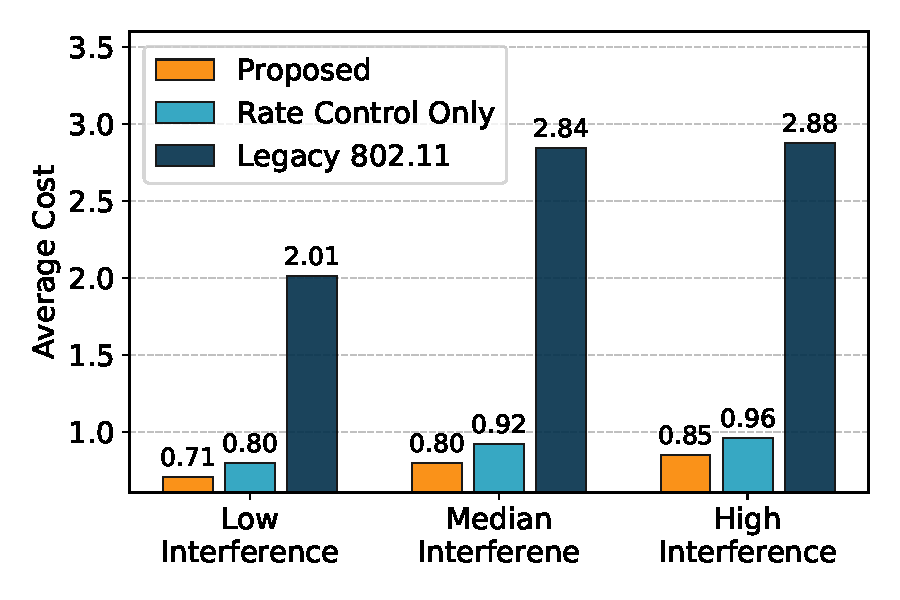
\includegraphics[width=\linewidth]{chapter3_after/Scenario 3-Average Cost 5.pdf}
        \caption*{(c) Scenario 3}
    \end{minipage} \\
    \begin{minipage}[b]{0.32\linewidth}
        \centering
        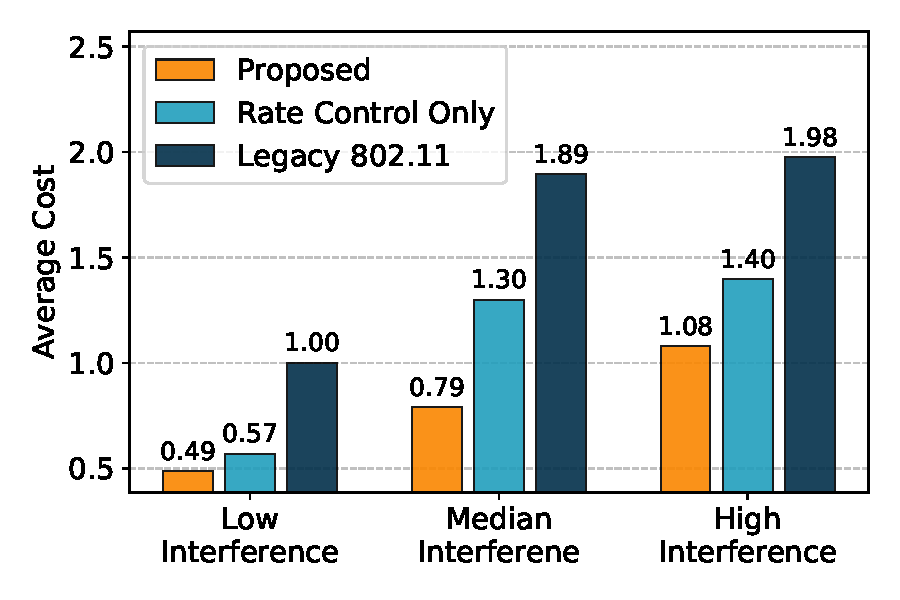
\includegraphics[width = 1\linewidth]{chapter3_after/Scenario 4-Average Cost 5.pdf}
        \caption*{(d) Scenario 4}
    \end{minipage}
    \begin{minipage}[b]{0.32\linewidth}
        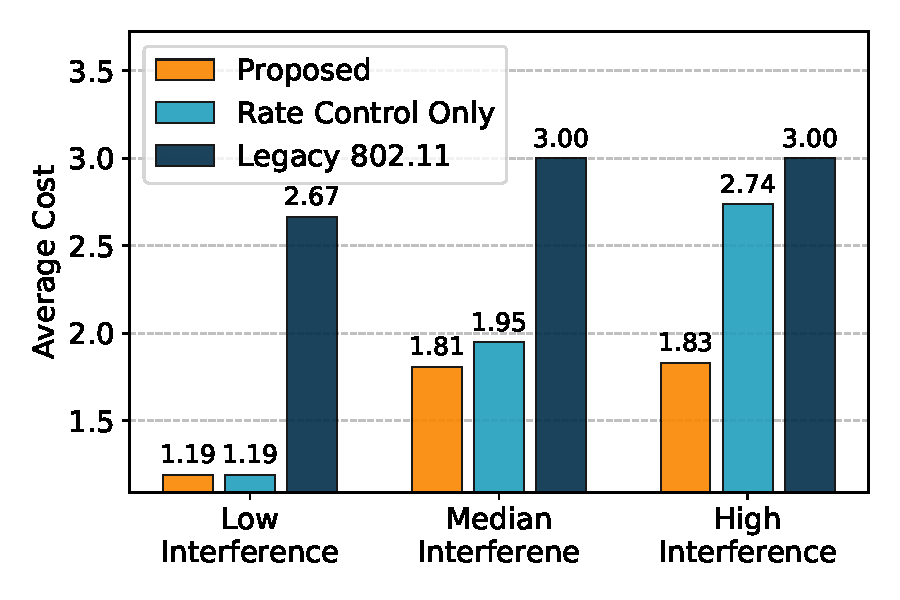
\includegraphics[width = 1\linewidth]{chapter3_after/Scenario 5-Average Cost 5.pdf}
        \caption*{(e) Scenario 5}
    \end{minipage}
    \caption{Comparing average costs across proposed algorithm, rate control only, and legacy 802.11 for evaluation scenarios from 1 to 5.}
    \label{fig:Average cost comparison of proposed algorithm in Scenario 1, 2, 3, 4 and 5.} % chktex 24
\end{figure*}


Based on dataset $\mathscr{S}^s$, the performance of the three traffic patterns are quantized into 3, 6 and 6 regions, respectively. Then, $15$ QoS imitators are trained with the tools of \textit{CUDA}\cite{cuda} and \textit{pytorch}\cite{NEURIPS2019_9015} according to Section~\ref{sec:Hybrid Q-Learning} with $\alpha=1$, $\beta=3$. Given the trained QoS imitators, the Q-network is further trained as elaborated in Section~\ref{sec:Hybrid Q-Learning} with $\omega=1/{r}^{(m,\max)}_{i,j}$.

The convergence of imitator and offline Q-network training is illustrated in \figurename~\ref{fig:imitator training loss} and \figurename~\ref{fig:scheduler training loss}, respectively. Specifically, the training loss of the imitator for the traffic scenario $3$ is illustrated in \figurename~\ref{fig:imitator training loss}, where the convergence performance of the proposed loss function in Equation (\ref{eq: imitator loss}) is compared with that of the standard MSE loss function. The proposed loss function is observed to ensure a significantly faster convergence rate. Specifically, 200 epochs are requested for convergence with the standard MSE loss function, while this number is reduced to 30 epochs with the proposed loss function.


\subsection{Performance Evaluation}
\label{Evaluation_Scenarios} % chktex 24
\begin{table}[!t]
    \centering
    \begin{tabular}{c|c|c|c} % chktex 44
    \specialrule{.1em}{.05em}{.05em} 
    Scenario  
    & 
    \begin{tabular}[c]{@{}c@{}}Traffic\\ Pattern\end{tabular}      
    & 
    Link                          
    & 
    \begin{tabular}[c]{@{}c@{}}Maximum Link Rate\\(Mbps)\end{tabular}  
    \\ 
    \hline % chktex 44
    \hline % chktex 44
    6   & 3    & $(u_3, u_0)$                           & 476       \\ \hline         % chktex 44
    7   & 3    & $(u_2, u_0)$                           & 424       \\ \hline         % chktex 44
    8   & 2    & $(u_2, u_0)$,$(u_3, u_0)$        & 400, 346  \\ \hline         % chktex 44
    9   & 3    & $(u_2, u_0)$,$(u_3, u_0)$        & 400, 346  \\ \hline         % chktex 44
    10  & 2    & $(u_1, u_0)$                           & 459       \\ \hline         % chktex 44
    11  & 3    & $(u_1, u_0)$                           & 459       \\ \hline \hline  % chktex 44
    \end{tabular}
    \caption{The maximum link rates of test scenarios from 1 to 6.\label{tab:Test Scenario}}
\end{table}

In this section, the performance of the proposed scheduling framework is showcased through evaluation across 11 distinct scenarios, with $3$ of them are listed in \figurename~\ref{fig:Testbed Setup}. These scenarios are subdivided into groups of 5 and 6 to assess both the performance and generalization capability of the proposed algorithm, respectively.

% Evaluate the performance of the proposed algorithm
In evaluating the algorithm performance, the first $3$ scenarios follow the traffic patterns where the maximum link rate of each link is $563$, $499$, and $572$ Mbps, respectively. 
Moreover, scenarios 4 and 5 follow the traffic patterns 2 and 3 with the maximum link rate reduction to $370$ Mbps of $(u_2, u_0)$.
Specifically, each traffic pattern is engaged with $3$ individual interference levels, namely \textit{Low Interference}, \textit{Medium Interference} and \textit{High Interference}, where the interference traffic rate is $0$, $50$ and $100$ Mbps, respectively. 

% Results
The average cost of the proposed algorithm, rate control only, and legacy 802.11 are compared in \figurename~\ref{fig:Average cost comparison of proposed algorithm in Scenario 1, 2, 3, 4 and 5.}. From the comparisons, the proposed algorithm outperforms both the rate control only algorithm and the legacy 802.11 mechanism in all five scenarios, which demonstrates the effectiveness of the proposed algorithm in the scheduling of combinations of delay-sensitive tasks and file delivery tasks.

\begin{figure}[!t]
    \centering
    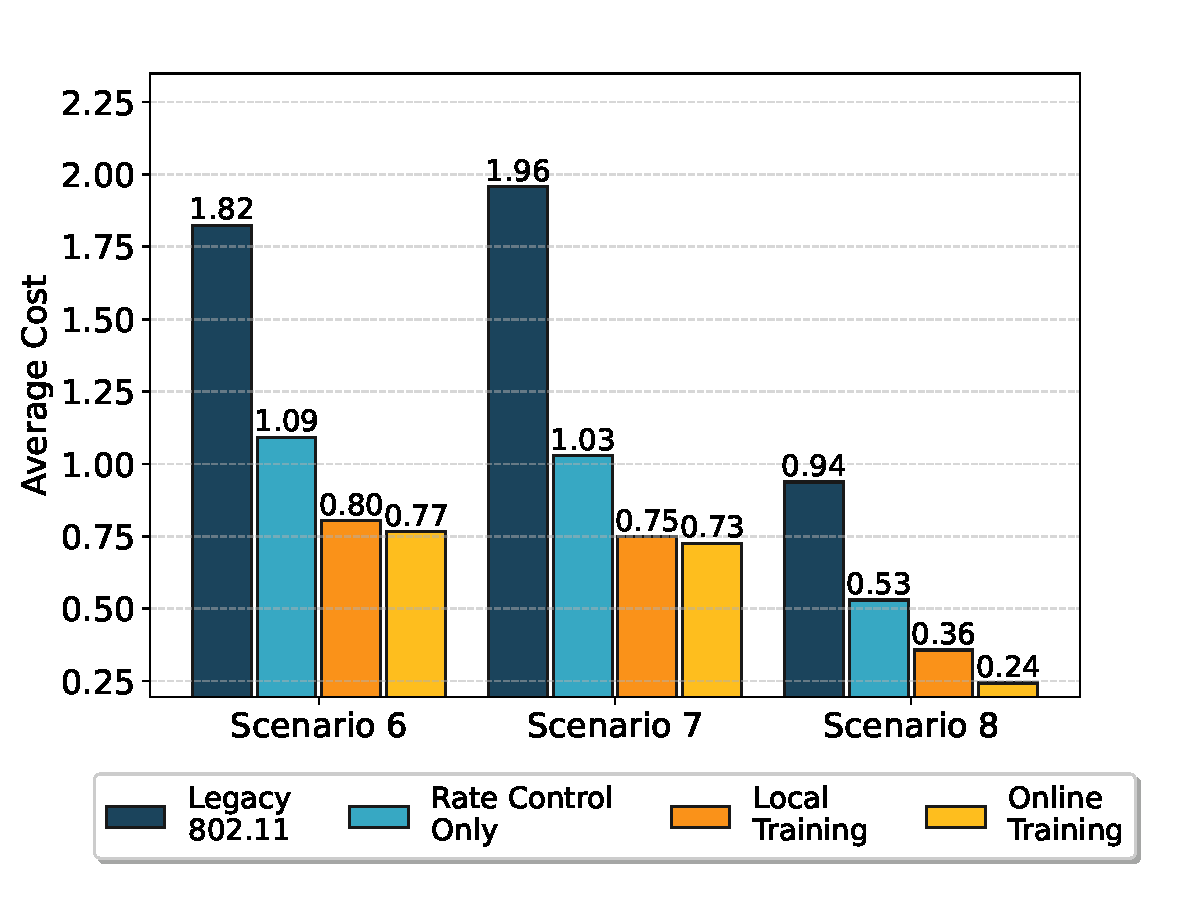
\includegraphics[width=\linewidth]{chapter3_after/test-case1-3.pdf} % chktex 8
    \caption{Comparing average costs across legacy 802.11, rate control only, Q-network trained offline (Local Training), and Q-network trained online (Online Training) for scenarios 6, 7, and 8.\label{fig:Test-changing interference-cost for test scenario 6, 7 and 8.}}
\end{figure}

\begin{figure}[!t]
    \centering
    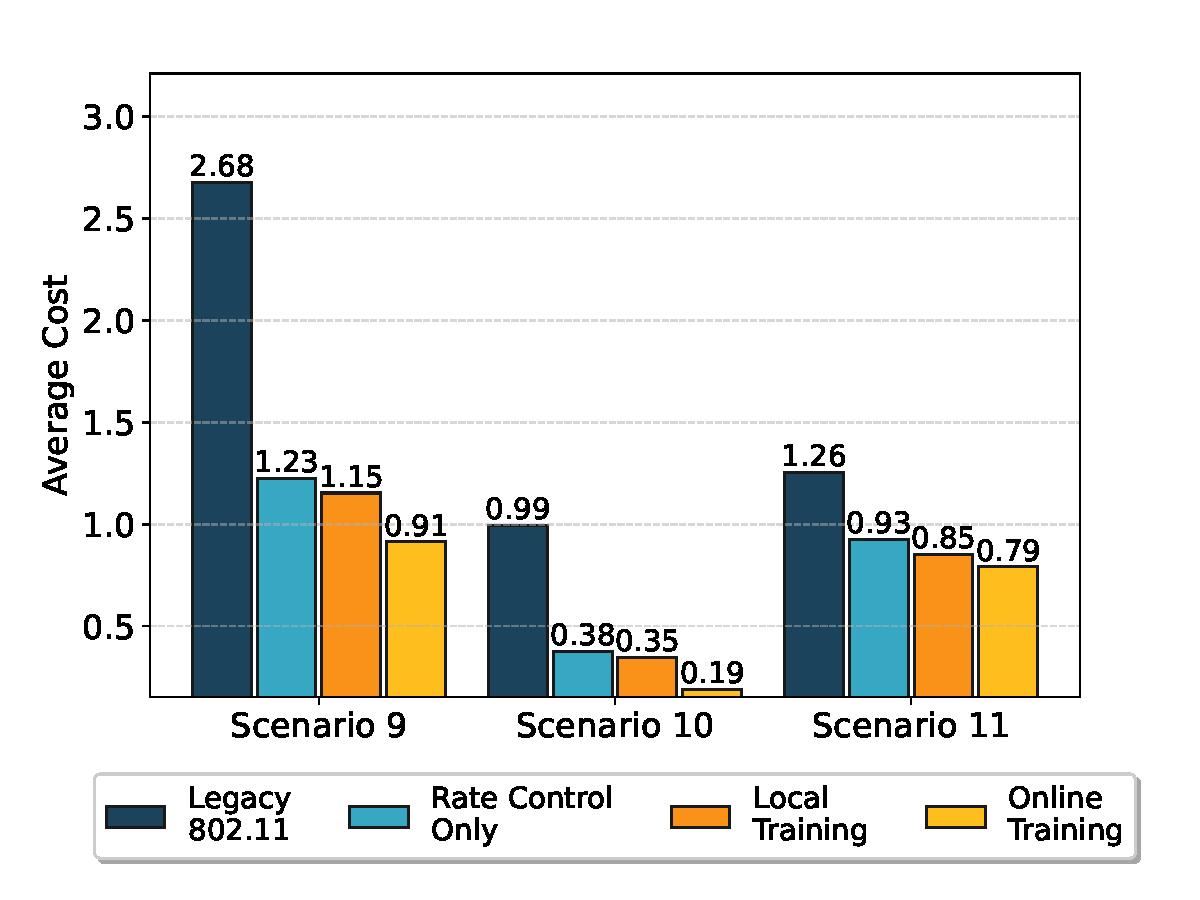
\includegraphics[width=\linewidth]{chapter3_after/test-case2-3.pdf} % chktex 8
    \caption{Comparing average costs across legacy 802.11, rate control only, Q-network trained offline (Local Training), and Q-network trained online (Online Training) for scenarios 9, 10, and 11.\label{fig:Test-changing interference-cost for test scenario 9, 10 and 11.}}
\end{figure}

%% Evaluate generation ability
In evaluating the generalization ability of the proposed algorithm, the proposed algorithm is further evaluated in $6$ test scenarios, where distance of link $(u_1,u_0)$, $(u_2,u_0)$ and $(u_3,u_0)$ are modified inducing a modified maximum link rate as Table~\ref{tab:Test Scenario}. During the evaluation, the locally trained scheduler is first used to control the transmission, which results in the \textit{Local Training} column. After that, the scheduler is further trained in an online manner following Equation (\ref{eq:online epolicy}), which results in the \textit{Online Training} column.

% Results
The average costs of the proposed algorithm and baselines in \figurename~\ref{fig:Test-changing interference-cost for test scenario 6, 7 and 8.} and \figurename~\ref{fig:Test-changing interference-cost for test scenario 9, 10 and 11.} showcase that localized training network is effective in scheduling under the unseen network condition, indicating a good generalization capability of the local trained network. 
Moreover, the scheduling under the online trained network results in an improved system performance, demonstrating the effectiveness of the online training mechanism.

\section{Summary}
\label{sec:chapter3_after-conclusion}
In this chapter, we consider the problem of optimizing the Quality of Service (QoS) of application-layer traffic in IEEE 802.11 networks. We propose a deep reinforcement learning-based channel access framework, {\algName}, which dynamically adjusts the Enhanced Distributed Channel Access (EDCA) parameters and throttles the throughput-hungry file streams to optimize the QoS of application-layer traffic.
We validate our proposed algorithm through commercial-off-the-shelf (COTS) hardware testbed.
Our results show that {\algName} can achieve a Pareto optimal of throughput and Round-Trip Time (RTT) for complex application-layer traffic under various network conditions.
% }

        %%% Conclusion
        % !TeX root = ../../main.tex

\chapter{Conclusions and Future Work}
\label{ch4}

In this thesis, we investigate the Approximate Markov Decision Process (AMDP) algorithm design for multi-agent edge computing and edge learning systems.
% The thesis is organized into two parts, where the theorems of the approximation solution frameworks are explored for infinite-horizon MDP problems in Part I and for finite-horizon MDP problems in Part II.
The proposed solution framework well addresses the challenges of the edge computing or edge learning applications appeared in each part.
The corresponding simulation results also verify the effectiveness of the proposed algorithms.
In this chapter, we firstly summarize the main contributions of this thesis and then discuss some potential research directions for future study.

\section{Conclusions}

\subsection{Low-complexity AMDP Algorithm Design in Edge Computing Systems}
In Part I, we consider the multi-agent job dispatching problem in an edge computing network with multiple APs and edge servers.
First of all, a centralized cooperative jobs dispatching problem with multiple access points (APs) and edge servers is considered in Chapter 2.
Due to the uncertain traffic in the network between APs and edge servers, the job uploading delay can not be predicted accurately.
We formulate the joint optimization of jobs dispatching at all the APs and all the time slots as an infinite-horizon MDP with discounted cost.
In order to avoid the curse of dimensionality, we introduce a low-complexity sub-optimal solution based on one-step policy iteration from a baseline policy.
In this chapter, a novel approximate MDP (AMDP) solution framework is proposed via one-step policy iteration over a baseline policy, where the analytical performance bound can be obtained.
Moreover, since the expression of the approximate value function is derived, the value iteration in conventional methods can be eliminated, which can essentially reduce the computation complexity.
Finally, it is shown by simulations that our proposed scheme has better performance than various benchmarks.

Furthermore, in Chapter 3, we extend the centralized scheduling problem to a decentralized scenario where the jobs dispatching is implemented in a distributed manner on multiple APs.
A broadcast-based signaling mechanism is introduced to facilitate the cooperation among distributed job dispatchers.
As the reception of updated and fully-observed global system state is discouraged due to the random transmission latency, the decentralized scheduling problem is formulated as a partially-observable MDP (POMDP) problem.
Hence, we propose a novel low-complexity solution framework for distributed job dispatching, based on which the optimization of job dispatching policy can be decoupled via an alternative policy iteration algorithm and a theoretical performance lower bound is obtained.
As for future work, we shall extend the proposed algorithm to one new scenario where the delay of collecting complete system state information at each AP is not negligible. Moreover, the memoryless distribution of uploading delay can also be generalized to arbitrary distribution.


\subsection{Low-complexity AMDP Algorithm Design in Edge Learning Systems}
In Part II, we extend the principle of the online algorithm design to the AMDP problems in edge learning systems.
\revise{
    Specifically, we consider both ``network-for-learning'' and ``learning-for-network'' scenarios in Chapter 4 and Chapter 5, respectively.
}%

In Chapter 4, we consider the edge federated learning system, where the {\IAVFullnames} ({\IAVs}) collect data from the environment and then upload the local training model to the edge server for aggregation.
Considering the limited communication resource and the randomness of vehicular mobility, the communication scheduling problem is proposed to achieve the trade-off between the training time and energy consumption.
We firstly develop a data-driven framework called {\fwName} to analyze the Markovian property of the vehicular mobility.
Then, we formulate the communication scheduling problem as a finite-horizon MDP problem.
To address the curse of dimensionality, we propose a novel two-time-scale approximate solution framework, where a centralized optimization of the transmission time and power is carried out at super-slot scale, while a decentralized fine-tuning of the transmission time is carried out at slot scale aware of the fast-change vehicular mobility.
A non-trivial performance lower bound is obtained with the proposed iterative policy update algorithm
The simulation results show that the proposed algorithm can achieve near-optimal performance with low complexity, and flexible trade-off between the performance and the computational complexity.
Furthermore, the hand-over among multiple base stations and the scheduling of multiple training epochs are not taken into consideration.

\revise{
In Chapter 5, we consider the ``learning-for-network'' scenario, where a learning-based scheduling framework is proposed and implemented to optimize the application-layer quality-of-service (QoS) of complex network traffics in a IEEE 802.11 WLAN system with unknown interference.
We jointly schedule the thoughput-hungry tasks of file delivery and delay-sensitive communication tasks, e.g., screen projection, by adjusting the contention window sizes and application-layer throughput throttling.
Due to the unknown interference and vendor-specific implementation of wireless NIC, a reinforcement learning method is proposed to learn the mapping from the historical scheduling parameters and QoS observations to the current scheduling action.
The experiment results on the commercial-off-the-shelf testbed show that the proposed framework can achieve a significantly better QoS than the conventional EDCA mechanism, and other heuristic algorithms.
}%

%=================================================================================================%
%=================================================================================================%
\section{Future Work}
In this section, we discuss some potential research directions for future study.
The focuses are put on two major aspects for theorems and applications, respectively, of the edge computing systems.
As for the applications, we focus on the emerging and potential problems for edge computing in sight of the state synchronization and multiple time-scale problems.
As for the theorems, we focus on the novel approximate online solution to large-scale multi-agent MDP.

\subsection{Emerging and Potential Problems for Edge Computing}
In the past few years, the resource allocation and task scheduling problems in edge computing have been widely studied in the literature.
With the prosperity of the 5G and the advance of Wi-Fi communication technology, the edge intelligent devices have also led to manifold applications aroused in the edge computing systems, such as edge caching, edge federated learning and etc.
However, the existing researches have little discussion on the general solution to the fundamental problem raised in such system: how to efficiently make and apply scheduling decisions in the large-scale multi-agent, especially in a decentralized manner?
In this section, we shed some light on the potential research directions for the edge computing systems.

\noindent\textbf{State Synchronization in Large-scale Network}
In Chapter 3, we consider the decentralized job dispatching problem in an edge computing network with multiple APs and edge servers.
A simple broadcast mechanism is introduced as the information sharing mechanism to facilitate the cooperation among distributed job dispatchers.
It is obvious that even with the extra information sharing, the reception of updated and fully-observed global system state is still unavoidable due to the transmission latency, and lower down the performance of the system.
The state synchronization among distributed agents is an inevitable problem in large-scale multi-agent systems.
In the literature, there have been some researches:
some works merely consider the evil effect of the outdated information and try to minimize the so-called information freshness in the system;
some works assume the agents compete with each other and argue that the equilibrium of the game could be achieved under certain strategy design;
some works assume the agents though cooperate in presence of partially observable information but the convergence could be guaranteed via online learning.
However, the disturbance of environmental dynamics and the heterogeneity of agents' behaviors (e.g., malicious attack) could lead to the failure of the above methods.
Hence, the state synchronization in large-scale multi-agent system is still an open problem and current engineering solutions are still based on the centralized control.

\noindent\textbf{Multi-level or Multiple Time-scale Problem}
In Chapter 4, we consider an edge federated learning system where the mobile vehicles collect data from the environment and then upload the local training model to the edge server for aggregation.
The edge server is responsible for the aggregation of the local training models and then broadcasts the global training model to all the participated mobile vehicles.
The communication scheduling problem is tackled in a multiple time-scale manner to address the fast-change of vehicular mobility.
This kind of multiple time-scale problem formulation or solution framework is seeking for more applications in the edge computing systems.
For example, in an edge caching system, the edge server may be responsible for minimizing the cache miss ratio in the long term, while fetching the popular contents in case of minimal energy consumption.
The joint optimization of the above two objectives could not be trivially decoupled and hence formulates a multi-level problem, where one algorithm is deployed at low-level for energy-efficient caching (short-term objective), while another algorithm at high-level, leverage its solution to achieve a minimum cache miss ratio (the long-term objective).
There are more potential applications of the multi-level or multiple time-scale problems when considering the computational complexity of the algorithm, when the time horizon of the system is much larger than the time scale of the algorithm.
This brings new challenges and opportunities for the online solution to large-scale multi-agent problem design.

\subsection{Novel Approximate MDP Solution Frameworks}
Throughout this thesis, we leveraged model-based MDP problem modeling and proposed several low-complexity approximate MDP solution frameworks for large-scale multi-agent problems.
The major contributions of these frameworks could be summarized into two aspects:
1) approximate value function evaluation, 2) iterative or alternative online policy update.
The two key ideas lead to the low-complexity solution framework with insightful analytical performance guarantee.
In this section, we discuss some potential research directions for the approximate MDP solution frameworks.

% \noindent\textbf{Deep Learning Endorsed Online Algorithm Design}
Recently, there is a trend of integrating deep learning with conventional online algorithm design, which is referred as \emph{online learning}.
The parameters of the conventional online algorithms are deemed as meta parameters, which can be optimized by deep learning algorithms.
The online learning algorithms have been widely studied in the literature, such as online convex optimization, online reinforcement learning and etc.
The deep reinforcement learning (DRL) is a de-facto successful online learning algorithm, which embraces the deep neural network to apply model-free value function approximation and policy optimization.
However, the model-free DRL algorithms are still lack of theoretical performance guarantee and fail to quickly adapt to the environment change due to the lack of model information.
Hence, the integration of model-based MDP problem modeling and model-free DRL algorithm design is a promising research direction for the approximate MDP solution frameworks.

% \noindent\textbf{Centralized Training with Decentralized Execution (CTDE)}
In the recent development of multi-agent reinforcement learning (MARL), the centralized training with decentralized execution (CTDE) paradigm has attracted much attention, which is a promising solution to distributedly cooperation among multiple agents without information sharing.
In the centralized training phase, a simulated environment is used to share information among agents, while in the decentralized execution phase, each agent chooses an action in accordance with only partially local information.
It is apparent that the simulated environment could be replaced by an approximated model-based MDP, and hence provide more theoretical performance analysis together with the convergence guarantee.

To conclude, the approximate MDP solution frameworks are still a promising research direction as one promising online solution to large-scale multi-agent systems.
The integration of deep learning and the CTDE paradigm in MARL are two potential research directions for the approximate MDP solution frameworks.

    \end{chapters}

    %% Back Matter
    \begin{backmatter}
        \printbibliography[heading=bibintoc,title=Bibliography]
    \end{backmatter}
\end{document}
